%\\\\\\\\\\\Document Properties\\\\\\\\\\\\\\\\\\\\\\\\\\\\\\\\\\\\\\\\\\\\\\\\\\\\\\\\\\\\\\\\\\\\\\\\\\\\\\\\\\\\\\\\\

    \documentclass[11pt,a4paper,reqno,titlepage]{report}
    \usepackage[HTML, table]{xcolor}
    \usepackage{colortbl}
    \usepackage[margin=6pc]{geometry}
    \usepackage[utf8]{inputenc}
    \usepackage[T1]{fontenc}
    \usepackage{amsfonts}
    \usepackage{amsmath}
    \usepackage{mathtools}
    \usepackage{amssymb}
    \usepackage{graphicx}
    \usepackage{tabularx}
    \usepackage{float}
    \usepackage{booktabs}
    \usepackage{titlesec,color}
    \usepackage{caption}
    \usepackage{enumitem}
    \usepackage{subcaption}
    \usepackage{pdfpages}
    \usepackage[hyphens]{url}
    \usepackage{array}
    \usepackage{notoccite}
    \usepackage{listings}
    \usepackage{siunitx}
    \usepackage[toc, titletoc]{appendix}
    \usepackage{longtable}
    \usepackage{makecell}
    \usepackage{fancyhdr} %header package
    \usepackage{multirow} %multirow for table
    \usepackage{verbatim}%I just added this to be able to make comments xoxo Steph PS if you want you can also change it to the comment package
    \usepackage[export]{adjustbox}
    \usepackage{acro} %list of abbreviations
    \usepackage{hyperref}
    \setcounter{LTchunksize}{50}% tex runs faster with larger chunks, 20 is default. Smaller chunk = less memory used. Using more memory is not possible since we don't wanna $$pay$$
    \usepackage{cleveref} %reference to multiple figures at the same time: \Cref{fig1,fig2,fig3} depicts Figures 1 to 3.
    \usepackage{glossaries}
    \usepackage{tablefootnote}
    \usepackage{adjustbox}
%   \usepackage{graphicx} %rotate text
    \usepackage{multirow} %multi row table
    \renewcommand{\chapterautorefname}{Chapter}
    \renewcommand{\sectionautorefname}{Section}
    \renewcommand{\subsectionautorefname}{Section}
    \renewcommand{\subsubsectionautorefname}{Section}
    \usepackage{tabulary}
    \usepackage{csquotes} %quote
    
    
    %!Danger! Leave 'arydshln' last! Add extra packages on top ^
    \usepackage{arydshln} %Adding dashlines in arrays \hdashline -- this should be loaded AFTER longtable, array, colortab and colortbl
    
    
%    \usepackage{savetrees} %this package tries to get everything on as little pages as possible
%\\\\\\\\\\\Document Properties\\\\\\\\\\\\\\\\\\\\\\\\\\\\\\\\\\\\\\\\\\\\\\\\\\\\\\\\\\\\\\\\\\\\\\\\\\\\\\\\\\\\\\\\

    %\usepackage[hidelinks, pdftitle={Project Plan Report Group 14}, pdfauthor={Group 14}, pdfsubject={AE3200 Design Synthesis Exercise}]{hyperref}



%\\\\\\\\\\\Setting-up Nomenclature Classes\\\\\\\\\\\\\\\\\\\\\\\\\\\\\\\\\\\\\\\\\\\\\\\\\\\\\\\\\\\\\\\\\\\\\\\\\\\\

    \usepackage{nomencl}
    \makenomenclature
    
    
    
    
\begin{comment}
    \usepackage{etoolbox}
    \renewcommand\nomgroup[1]{%
        \item[\bfseries
            \ifstrequal{#1}{G}{Greek Symbols}{%
            \ifstrequal{#1}{B}{Roman Symbols}{%
            %ADD MORE CLASSES HERE (Order does not matter, LaTeX will sort classes Based on !Class Reference
            %\ifstrequal{#1}{!Class Reference}{!Class Name}{%
            %\ifstrequal{#1}{!Class Reference}{!Class Name}{%
            %\ifstrequal{#1}{!Class Reference}{!Class Name}{%
            \ifstrequal{#1}{A}{Abbreviations}{}}}%
        ]}
\end{comment}






    % This argument will add the units
    \newcommand{\nomunit}[1]{%
    \renewcommand{\nomentryend}{\hspace*{\fill}[#1]}}
    
    %Renames Nomenclature to List of Symbols
    \renewcommand{\nomname}{List of Symbols}
               

%\\\\\\\\\\Table Spacing & Layout Parameters\\\\\\\\\\\\\\\\\\\\\\\\\\\\\\\\\\\\\\\\\\\\\\\\\\\\\\\\\\\\\\\\\\\\\\\\\\\

    \renewcommand{\arraystretch}{1.2}
    \newcolumntype{C}{>{\centering\arraybackslash}X} %For tabularX
    \newcolumntype{L}{>{\raggedright\arraybackslash}X} %For tabularX
    \newcolumntype{R}{>{\raggedleft\arraybackslash}X} %For tabularX
    \newcolumntype{b}{X} %For tabularX
    \newcolumntype{s}{>{\hsize=.5\hsize}X} %For tabularX
    %the columns listed 
    
    %this section defines a command that lets an entire row be put in a font/bold/anything
    %\newcolumntype{=}{>{\global\let\currentrowstyle\relax}}
    %\newcolumntype{^}{>{\currentrowstyle}}
    %\newcommand{\rowstyle}[1]{\gdef\currentrowstyle{#1}%
    %#1\ignorespaces 
    %%%%%%%%%%%%%%%%%%%%%%%%% Who added this? This FUCKS UP the report.
    

 
    %Changes parameters for \hdashline to make the dashes into dots:
    \setlength\dashlinedash{0.2pt}
    \setlength\dashlinegap{1.5pt}
    \setlength\arrayrulewidth{0.3pt}
    
    
%\\\\\\\\\\\Set Document Layout & Title Margins\\\\\\\\\\\\\\\\\\\\\\\\\\\\\\\\\\\\\\\\\\\\\\\\\\\\\\\\\\\\\\\\\\\\\\\\

    \titlespacing*{\chapter}{0pt}{-25pt}{10pt}
    \definecolor{gray75}{gray}{0}
    \newcommand{\hsp}{\hspace{3pt}}
    \titleformat{\chapter}[hang]{\Huge\bfseries}{\thechapter\hsp\textcolor{gray75}\hsp}{10pt}{\Huge\bfseries}

%\\\\\\\\\\\Rename Bibliography to References\\\\\\\\\\\\\\\\\\\\\\\\\\\\\\\\\\\\\\\\\\\\\\\\\\\\\\\\\\\\\\\\\\\\\\\\\\

    \usepackage[
    backend=biber,
    style=numeric,
    citestyle=numeric,
    sorting=none
    ]{biblatex}
    \addbibresource{references.bib} %Bibliography File
    \newcommand{\BibliographyName}{Bibliography} %Name of Biblography
    
%\\\\\\\\\\\Changing Footnote Counts to Arabic\\\\\\\\\\\\\\\\\\\\\\\\\\\\\\\\\\\\\\\\\\\\\\\\\\\\\\\\\\\\\\\\\\\\\\\\\\

    \renewcommand{\thefootnote}{\arabic{footnote}}

%\\\\\\\\\\\Putting Chapter Titles, Page Number and Line in Header Section\\\\\\\\\\\\\\\\\\\\\\\\\\\\\\\\\\\\\\\\\\\\\\\\\\\\\\\\\\\\\\\\\\\\\\\\\\

    \pagestyle{fancy}
    \fancyhf{}
    \rhead{\thepage} %Puts a page number on the right side of a header
    \lhead{\leftmark} %Puts a chapter number and name on the left side of a header
    \rfoot{}
    
    
    

%\setlist[description]{leftmargin=1cm,labelindent=1cm}
 
    



%Document
\begin{document}  
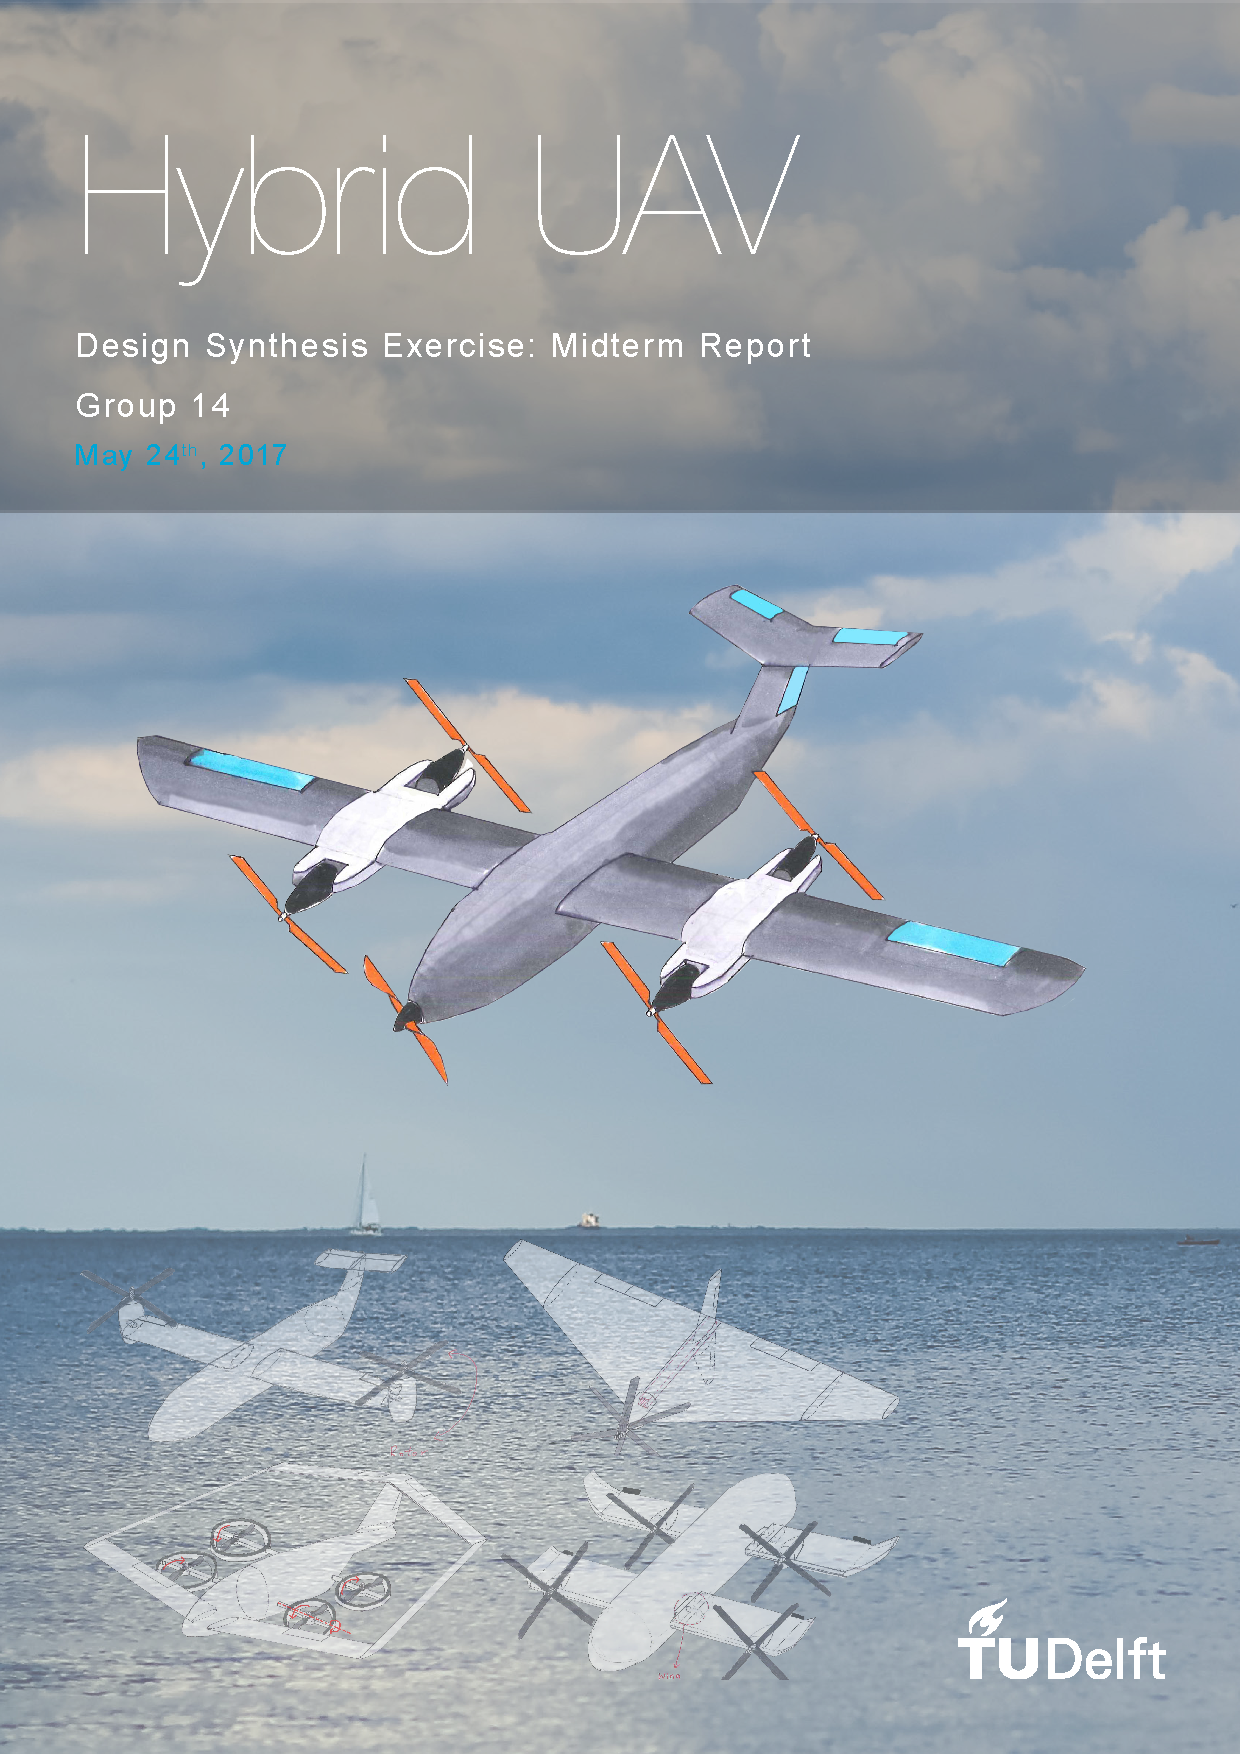
\includepdf[pages={1}]{title.pdf}
\setlength{\parindent}{0cm} % No indent

%%%%%%%%%%%%%%%%%%%%%%%%%%%%%%%%%%%%%%%%%%%%%%%%%%%%
%%%%%%%%%%%%%%%%%%%%%%%%%%%%%%%%%%%%%%%%%%%%%%%%%%%%
%We should enter an empty page here, otherwise the inner cover will be printed on the back side of the cover page.Okay!
%%%%%%%%%%%%%%%%%%%%%%%%%%%%%%%%%%%%%%%%%%%%%%%%%%%%
%%%%%%%%%%%%%%%%%%%%%%%%%%%%%%%%%%%%%%%%%%%%%%%%%%%%


%Inner Title Page
\newgeometry{margin=6pc} %Change Title-Page Margin Differently
\begin{titlepage}
\begin{center}

\textsc{\LARGE Delft University of Technology}\\[1.5cm]

\includegraphics[scale=0.45]{TU_Delft_logo_RGB.png}\\[0.5cm]
\textsc{\Large AE3200 - Design Synthesis Exercise}\\[0.5cm]
{\huge\textbf{Midterm Report} \\[.2cm] \Large\textsc{Version 1.0}\\[1.0cm]}

\begin{minipage}[t]{0.4\textwidth}
\begin{flushleft} \large
\emph{Authors:}\\
    4384385  Jong, C.P.L. de\\
    4221699  Kim, M.\\
    4376161  Lee, J.J. van de\\
    4371321  Lovell-Prescod, G.H.\\
    4308220  Ruland, O.L.\\
    4344499  Sokolowski, P.M.\\
    4279832  Steiner, L.F.\\
    4364228  Wellens, L.\\
    4280806  Wheeler, K.\\
    4381726  Wiechers, S.M.G.
    

\end{flushleft}
\end{minipage}
\begin{minipage}[t]{0.4\textwidth}
\begin{flushright} \large
\emph{Supervisors:} \\
    Jos Sinke\\
    Sebastian Rapp\\
    Erik-Jan van Kampen
    
    
\end{flushright}
\end{minipage}
\vfill
\textit{Cover Image:} Pexels\\
\small
\url{}

\end{center}
\end{titlepage}
\restoregeometry

%Document Part I:
\begingroup
\pagenumbering{roman} % Roman numbering
    
    %Summary
    \chapter*{Preface}

This report is the third document in a series of reports about the design of a Hybrid Unmanned Aerial Vehicle (UAV). The first document was the project plan report, followed by the baseline report. In the first document, the organisation and planning of the project was described, and the first steps were taken in the design process. In the baseline report, a market analysis is made and a large number of concepts was presented. From these, five concepts were chosen, which are further analysed in this report. This report will be followed up by a final report that discusses the preliminary design of the chosen concept.

Group 14 would like to thank Ir. J. Sinke, Dr.Ir. E. van Kampen and Ir. S. Rapp for their advise, professional assistance and feedback. 
    \chapter*{Summary} %PLEASE STOP CHANGING THIS

%Outline of background (why are we writing this)
\begin{comment}
- UAV market is growing
- Dull, dirty, dangerous missions
New technologies such as improved Lithium batteries allow the UAVs to be developed further and further. Since a large amount of missions is either dull, dirty or dangerous, a demand for drones makes sense. Such boring or life-threatening missions, that have been performed using manned aircraft in the past, are a great opportunity for UAVs.  
\end{comment}

The Unmanned Arial Vehicle (UAV) market is growing\footnotemark, as the field of application becomes increasingly diverse \cite{baseline}. New technologies such as improved lithium batteries allow the UAVs to be designed lighter and smaller, or to increase their range. A large amount of missions is either dull, dirty or dangerous, and are therefore better executed by UAVs instead of manned aircraft. 

\footnotetext{\url{http://www.businessinsider.com/uav-or-commercial-drone-market-forecast-2015-2?international=true&r=US&IR=T}, Accessed 22-05-2017} 


The spectrum of missions that can be performed by UAVs is broad. On the one end are small and inexpensive UAVs that are used by consumers and companies alike. On the other end are very large military UAVs, which have an intercontinental range and endurance in the order of days. Many missions require both operation without extensive facilities, while also achieving high-speed flight. This is why a Hybrid UAV would be very useful: it could be operated from virtually anywhere as it does not require a runway, but has the flight performance of a conventional aircraft.

%Purpose of the report
\begin{comment}
- Compare concepts
- Find optimal concept that is able to meet the requirements
\end{comment}

In this report, a trade-off is performed between five concepts in order to determine what type of Hybrid UAV layout is optimal for the given requirements. From these requirements, the most important ones are a maximum speed of 200 km/h, an endurance of at least one hour, a payload carrying capacity of 10 kg and the vertical take-off and landing. The concepts that are compared are a Tailsitter, a Tandem configuration, a Prandtl boxed wing configuration, an aircraft with tilting rotors and a hybrid quadcopter design. Based on a number of criteria, which in turn were based on the requirements, the concepts are compared to each other. 


It was found that overall, the Tandem concept performed the worst. It especially lacked on flight performance and sustainability. The Tiltrotor concept did not perform well either and lacked on the same points plus production cost. The Prandtl Box concept performed quite well, and scored very well on development risk, reliability and performance. But the design that is expected to meet all requirements the best is the Winged Quadcopter, that performed very well compared to the others on each point. Because of this, the decision has been made to use the Winged Quadcopter to continue the design process.



%Concepts used in TO, criteria
\begin{comment}
- Describe all 5 concepts, refer to where they can be found
- Summarise all criteria
\end{comment}

%Result of TO, elaborate on concept
\begin{comment}
- Explain result and why
- Further elaborate on concept
\end{comment}

















 % Summary
    \addcontentsline{toc}{chapter}{Preface}
    \addcontentsline{toc}{chapter}{Summary} % Adding the Summary to the ToC

    %Table of Contents
    \setcounter{tocdepth}{1} %this is supposed to show chapters and sections only on toc (tocdepth of 1), but what's the issue? - bryan because its easy for quality control to check the structure of the report, personally i also like to see the sections in the toc - lotte
    \renewcommand{\contentsname}{Table of Contents}
    \tableofcontents
    \thispagestyle{empty}

    \clearpage

    %List of Symbols
    \printnomenclature[50pt]
    \addcontentsline{toc}{chapter}{List of Symbols}

    %List of Figures
    \listoffigures
    \addcontentsline{toc}{chapter}{List of Figures}

    %List of Tables
    \listoftables
    \addcontentsline{toc}{chapter}{List of Tables}
\endgroup
\clearpage

%Document Part II:
\begingroup
\pagenumbering{arabic}

    %Chapters:  LEAVE ALL IN I'M READING FOR THE CONCLUSION AND IT IS ALSO NEEDED FOR DEBUGGING
    %\chapter{SAMPLE}
\pagenumbering{arabic}

This template has been developed for the [AE3200] Design Synthesis Exercise. \texttt{THIS TEMPLATE CANNOT BE USED WITHOUT EXPRESSED PERMISSION FROM:} \c{S}an K{\i}lk{\i}\c{s} and Munyung Kim

\section{Tables \& Figures}
An example \autoref{tab:exampletable} and an example \autoref{fig:flame} can be found in this section. When you label tables or figures, make sure to use `tab:name' or `fig:name'. For inserting 2+ figures in a row, look at the formatting of Figure \autoref{fig:sbs}. Using the \texttt{autocite} command negates the need for manually typing `Table' or `Figure'. The syntax is as follows, note that the `tab' in `tab:exampletable' is not necessary for \texttt{autocite} and is purely for organizational reasons.

\begin{verbatim}
    \autocite{tab:exampletable}
\end{verbatim}

The Tables below use the package \texttt{tabularx} which adjusts column spacing automatically to fit the table within the margins of the page. The syntax is as follows where 'L' is for Left Aligned, 'C' for Centered, and 'R' is for Right Aligned. If you want to make a longer table, unfortunately \texttt{tabularx} cannot be used :( \#sad. Some tweaking is required on sizing, but apart from that, you can still make gorgeous tables (see below):

\begin{verbatim}
    \begin{tabularx}{\textwidth}{L C C C}
\end{verbatim}

In order to keep up the same appearance for all tables use the commands \texttt{toprule}, \texttt{midrule}, \texttt{bottomrule}, and \texttt{hdashline} to create the horizontal lines. NO VERTICAL LINES ARE ALLOWED!

\begin{table}[H]
	\centering
	\caption{Example Table}
	\label{tab:exampletable}
	\begin{tabularx}{\textwidth}{L C C C} %'L' for Left Aligned, 'C' for Centered, 'R' for Right Aligned
	    \toprule\
		\textbf{Component}				& \textbf{Mass [$\text{kg}$]}	&\textbf{Location [$\text{m}$]} & \textbf{Location [\% MAC]}   \\ \toprule
		Wing 							& 425.4 						& 5.74 							& 40.00\\\hdashline
		Main Landing Gear 				& 243.1 						& 5.82 							& 45.00 \\\hdashline
		Fuel System 					& 80.74 						& 5.91 							& 50.00 \\\hdashline
		Flight Control System 			& 48.61 						& 6.08 							& 60.00	\\\hdashline
		Hydraulics 						& 4.660 						& 6.08 						    & 60.00 \\\hdashline
		\textbf{Wing Group} 			& \textbf{802.5} 				& \textbf{5.80} 				& \textbf{43.85}\\ \midrule
		Fuselage 						& 265.2 						& 5.74 	                        & 40.00 \\\hdashline
		Engine 							& 409.4 						& 1.64 							& - \\\hdashline
		Avionics 						& 490.9 						& 4.39 							& - \\\hdashline
		H. Tail 						& 42.93 						& 13.2 						    & - \\\hdashline
		V. Tail 						& 66.43 						& 12.6 						    & - \\\hdashline
		Nose Gear						& 54.58 						& 2.50 							& - \\\hdashline
		Electrical 						& 217.4 						& 6.16 							& 67.12 \\\hdashline
		AC \& Anti-Ice 					& 215.7 						& 6.16 							& 67.12 \\\hdashline
		Furnishings 					& 241.5 						& 6.16 							& 67.12 \\\hdashline
		\textbf{Fuselage Group} 		& \textbf{2004} 				& \textbf{5.01} 				& \textbf{-2.32} \\ \midrule
		\textbf{OEW C.G.} 				& \textbf{2806} 				& \textbf{5.24} 				& \textbf{10.88} \\ \bottomrule
	\end{tabularx}
\end{table}

Here's how you make a long table that breaks automatically over pages (just copy this if you want to make one)
\begin{verbatim}
    \begin{longtable}[]{l l p{.3\linewidth}} %'l' is left aligned, but for pieces with text use p{size} to define column width
        \caption{Long tables are awesome\label{tab:haha_fun}}\\ %putting label below gives an error and you need the enter\\
        %now define the layout of the table
        \toprule
        This is the text that only will go at the beginning of your table (so just once)
        \\ \midrule
        \endfirsthead
        %%%%
        \caption[]{(continued)}
        \toprule
        This is something that goes on top of each part on every page the table spans
        \\ \midrule
        \endhead
        %%%%
        \midrule \endfoot
        \bottomrule \endlastfoot
        Now & this & is\\
        the & place & where\\
        the & table & goes \\
    \end{longtable}
\end{verbatim}

\begin{table}[H]
	\centering
	\caption{Example Table II}
	\label{tab:exampletableII}
    \begin{tabularx}{\textwidth}{C C C C C C C C} %'L' for Left Aligned, 'C' for Centered, 'R' for Right Aligned
    \toprule\
    {$m$} & {$\Re\{\underline{\mathfrak{X}}(m)\}$} & {$-\Im\{\underline{\mathfrak{X}}(m)\}$} & {$\mathfrak{X}(m)$} & {$\frac{\mathfrak{X}(m)}{23}$} & {$A_m$} & {$\varphi(m)\ /\ ^{\circ}$} & {$\varphi_m\ /\ ^{\circ}$} \\ \toprule
    1  & 16.128 & +8.872 & 16.128 & 1.402 & 1.373 & -146.6 & -137.6 \\ \hdashline
    2  & 3.442  & -2.509 & 3.442  & 0.299 & 0.343 & 133.2  & 152.4  \\ \hdashline
    3  & 1.826  & -0.363 & 1.826  & 0.159 & 0.119 & 168.5  & -161.1 \\ \hdashline
    4  & 0.993  & -0.429 & 0.993  & 0.086 & 0.08  & 25.6   & 90     \\ \midrule
    5  & 1.29   & +0.099 & 1.29   & 0.112 & 0.097 & -175.6 & -114.7 \\ \hdashline
    6  & 0.483  & -0.183 & 0.483  & 0.042 & 0.063 & 22.3   & 122.5  \\ \hdashline
    7  & 0.766  & -0.475 & 0.766  & 0.067 & 0.039 & 141.6  & -122   \\ \hdashline
    8  & 0.624  & +0.365 & 0.624  & 0.054 & 0.04  & -35.7  & 90     \\ \midrule
    9  & 0.641  & -0.466 & 0.641  & 0.056 & 0.045 & 133.3  & -106.3 \\ \hdashline
    10 & 0.45   & +0.421 & 0.45   & 0.039 & 0.034 & -69.4  & 110.9  \\ \hdashline
    11 & 0.598  & -0.597 & 0.598  & 0.052 & 0.025 & 92.3   & -109.3 \\ \bottomrule
    \end{tabularx}
\end{table}

\begin{figure}[H]
    \centering
    
\includegraphics[width=0.3\textwidth]{SAMPLE/Figures/flame.jpg}
    \caption{TU Delft Logo Flame}
    \label{fig:flame}
\end{figure}

\begin{figure}[H]
\centering
\begin{subfigure}[b]{0.5\textwidth}
  \centering
  
\includegraphics[width=.85\textwidth]{SAMPLE/Figures/flame.jpg}
  \subcaption{TU Delft Logo Flame}
  \label{fig:flame1}
\end{subfigure}%
\begin{subfigure}[b]{0.5\textwidth}
  \centering
  
\includegraphics[width=.85\textwidth]{SAMPLE/Figures/flame.jpg}
  \subcaption{TU Delft Logo Flame}
  \label{fig:flame2}
\end{subfigure}
\caption{Two Figures Side-by-Side} %Main Caption
\label{fig:sbs}
\end{figure}


\section{References \& Citations}
The \texttt{biblatex} package is used for references with the default `numeric' style for in-text citations and references. The references sorting style is set to `none' meaning that the references are sorted by the order in which they appear in text. A sample file \texttt{samplerefs.bib} is included to help when dealing with different types of publications. For using footnotes, use the footnote code at a location you wish to insert a footnote \footnote{This is an example}.

\begin{verbatim}
    \cite{citationtag}
\end{verbatim}

\begin{verbatim}
    \cite{\footnote{}}
\end{verbatim}



\section{Equations \& Nomenclature}
Starting with variables, you need to use a nomenclature code when you introduce a variable for the FIRST time, such that the variable is listed on the list of symbols. An example is given in Equation \autoref{eq:exampleeq}.

\begin{equation}
\label{eq:exampleeq}
    L = \frac{1}{2}\rho V^2 S \cdot C_{L}
\end{equation}

\nomenclature[A]{ABCD}{ABCD}
\nomenclature[B]{$C_L$}{Lift Coefficient \nomunit{-}}
\nomenclature[B, 01]{$V$}{Velocity \nomunit{\si{kg.m^{-1}}}}
\nomenclature[B, 02]{$S$}{Wing Area \nomunit{\si{m^{2}}}}
\nomenclature[G]{$\rho$}{Density of Air \nomunit{\si{kg.m^{-3}}}}

The the list of symbols for the above equation were generated with the code below:

\begin{verbatim}
    \nomenclature[A]{ABCD}{ABCD}
    \nomenclature[B]{$C_L$}{Lift Coefficient \nomunit{-}}
    \nomenclature[B, 01]{$V$}{Velocity \nomunit{\si{kg.m^{-1}}}}
    \nomenclature[B, 02]{$S$}{Wing Area \nomunit{\si{m^{2}}}}
    \nomenclature[G]{$\rho$}{Density of Air \nomunit{\si{kg.m^{-3}}}}
\end{verbatim}






 this is a sample chapter 
    \chapter{Introduction}

The ultimate goal of this hybrid Unmanned Aerial Vehicle (UAV) project is to design a UAV that combines the capabilities of high velocity horizontal flight with vertical take-off and landing (VTOL) and hovering. The project aims document and present an efficient Hybrid UAV design which can be controlled remotely within visual line of sight (VLOS) with the capability of beyond visual line of sight (BVLOS) control in the future. Derived from the aforementioned goal is the project objective statement (POS) which summarises the goal of the project and the steps required to achieve it in one statement and is characterised as follows.

\nomenclature[A]{UAV}{Unmanned Aerial Vehicle}
\nomenclature[A]{VTOL}{Vertical Take-off and Landing}
\nomenclature[A]{VLOS}{Visual Line of Sight}
\nomenclature[A]{BVLOS}{Beyond Visual Line of Sight}
\nomenclature[A]{POS}{Project Objective Statement}
\nomenclature[A]{MNS}{Mission Needs Statement}

\begin{quote}
\begin{itshape}
Design and optimise a Hybrid UAV that meets requirements and constraints by using project management and systems engineering tools, by a team of 10 students within 11 weeks.
\end{itshape}
\end{quote}

The midterm report serves to document both the trade-off and the analyses necessary to perform it. The required functions of the Hybrid UAV identified and defined in the baseline report form the foundation upon which the requirements and constraints can be determined \cite{baseline}. These functions and requirements follow indirectly from the mission need statement (MNS) which concisely defines what the goal of the design is and is characterised as follows.

\begin{quote}
\begin{itshape}
Carry out both supervised and autonomous monitoring and transport missions, comprising vertical take-off and landing, and sustained high-velocity horizontal flight.
\end{itshape}
\end{quote}

In \autoref{ch:proj_orga} the structure of the group is defined as well as the plan of attack of the whole project. This includes the work flow diagram (WFD), the work breakdown structure (WBS) and the Gantt chart. \autoref{ch:requ} presents the requirements and constraints on the system as well as classifies these requirements as killer, key or driving. In \autoref{ch:concepts} the five concepts that further analysis will be conducted on are presented and \autoref{ch:trad_off} presents the trade-off of the said concepts. In Chapters \ref{ch:perf_analy} to \ref{ch:grou_hand} the analyses of the trade-off criteria are presented. In each of these chapters either a sub-trade-offs is conducted or a grading system is defined. The N2 charts are introduced in \autoref{ch:n2_char} and characterise the interfaces between the subsystems as well as the relationships between subsystems during operation. A life cycle assessment procedure is presented in \autoref{ch:sustaindev} which lays down the framework to assess the sustainability of the whole process. In \autoref{ch:tech_risk_asse} the risk of of each concept not meeting the requirements is assessed and possible mitigation strategies are presented. \autoref{ch:prod_plan} presents an assembly based production plan which, should the UAV go into production, provides information that on the production process. \autoref{sec:ol} on operations and logistics focuses on defining the support facilities that need to be in place as well as the activities that need to be carried out so that the UAV can perform the prescribed missions. In \autoref{ch:layo_and_conf} the internal layout of the main subsystems is displayed along with the communication flow which defines the flow of information, data and commands through the system. Lastly, \autoref{ch:v_and_v} the verification and validation procedures are presented.

\nomenclature[A]{WFD}{Work Flow Diagram}
\nomenclature[A]{WBS}{Work Breakdown Structure}
    \chapter{Project Organisation}
\label{ch:proj_orga}
%checked by Bryan @2102

A team must have a solid team structure such that team members can work at maximum efficiency. After defining and distributing tasks, team rules need to be formulated for managing the team. In addition, the work must be approached in a structured manner, therefore a work flow and schedule must be created.

The team structure and organisation management are elaborated in \autoref{sec:orga_struc}, whilst the Work Flow Diagram (WFD), Work Breakdown Structure (WBS), and the Gantt chart are shown in \autoref{sec:work_appr}. 


\section{Organisational Structure}
\label{sec:orga_struc}
In this section, the non-technical and technical tasks will be described and assigned to each team member. Relations between tasks can be found in an organogram.

\subsection{Organogram}

The organogram of the team can be seen in \autoref{fig:organogram}. 
The organogram is divided into a management department, an engineering department and a chairman. 
The engineering department is responsible for designing a product or a system. It consists of specialised units as following: cost engineers, reliability engineers, performance engineers, control \& stability engineers, sustainability engineers, ground handling engineers and risk engineers.
The management department mainly manages the team and organisational tasks. It consists of a time manager, a secretary, administrators, a sustainability manager, quality control managers and system engineers. The chairman connects the engineering and management departments with great communication skills and a solid overview of project phases in both organisational and technical aspects.


\begin{figure}[H]
    \centering
    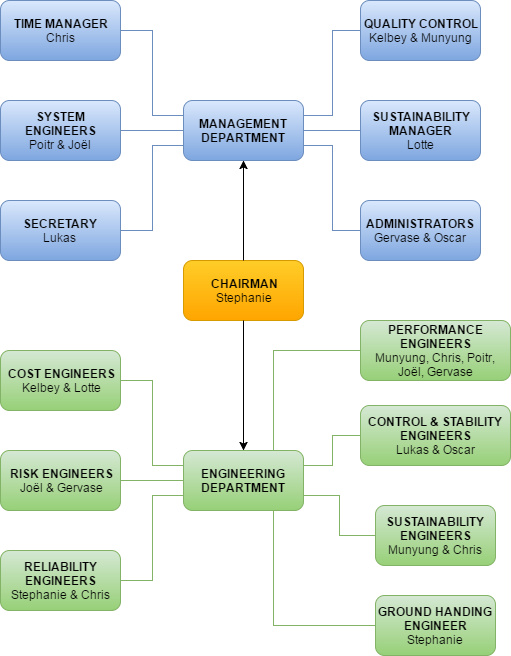
\includegraphics[width=0.5\textwidth]{ProjectOrganisation/Figures/Organogram}
    \caption{Organisational breakdown structure}
    \label{fig:organogram}
\end{figure}

\subsection{Non-Technical Task Division}
Description and distribution of non-technical tasks for corresponding roles can be seen in \autoref{tab:nttdiv}.

\begin{table}[H]
    \centering
    \caption{Description and distribution of the non-technical tasks within the team}
    \label{tab:nttdiv}
    \begin{tabular}{p{2.7cm}lp{10cm}}
        \toprule \
        \textbf{Role}      & \textbf{Name}     & \textbf{Assigned Tasks} \\
        \toprule \
        Chairman & Stephanie & - Leads meetings \\
         &  & - Is a contact person for external communication \\
         &  & - Has broad overview of overall progress and group dynamics \\
         &  & - Monitors the functioning of the organisation \\
         &  & - Takes action when the organisation or individuals perform sub-optimal on non-technical tasks \\ \hdashline
        Quality Control & Munyung & - Check lingual consistency of the report \\
                        & Kelbey & - Check compliance with writing procedures \\
         &  & - Resolve latex syntax errors \\
         &  & - Check spelling and grammar \\
         &  & - Check if deliverables are present \\ 
         &  & - Develop a quality control system \\ \hdashline
        Secretary & Lukas & - Makes notes during internal and external meetings \\
         &  & - Documents action points and questions for coaches and/or project supervisor \\ \hdashline
        Systems & Piotr & - Make sure that SE tools are being implemented correctly \\
        Engineer         &  Joël & - Make sure that SE tools are used throughout the project \\
        &  & - Make sure that SE tools are being updated continuously \\ \hdashline
        Time Manager & Chris & - Keeps track of the planning \\
                     &       & - Makes sure that the task management system (Trello) is up to date \\
         &  & - Spots delays early on \\
         &  & - Communicates with chairman to minimize further delays by reallocating human resources \\ \hdashline
        Sustainability & Lotte & - Monitors the overall sustainability of the design \\
        Manager &   & - Brings sustainability to the attention of the subsystem designers \\
         &  & - Ensures that the strategy for manufacturing, support and end-of-life solution of the product are sustainable \\ \hdashline
        Administrators & Oscar & - Structure and monitor file directories \\
         & Gervase & - Oversee the product data management system \\
         &  & - Implement changes in the master document \\
         &  & - Keep track of released versions of documents \\ \bottomrule
    \end{tabular}
\end{table}

\subsection{Technical Task Division}
Description and distribution of technical tasks for corresponding roles can be seen in \autoref{tab:ttdiv}. A division by trade-off criteria is chosen instead of a division by concepts, since it is efficient for team members to research one technical domain and apply it to each concept. Furthermore, biased analysis can be avoided, as team members cannot apply their preferences to analysis of a specific concept when tasks are divided based on criteria. 

The technical roles are included in the engineering department in the organogram.

\begin{table}[H]
    \centering
    \caption{Distribution and Description of Technical Tasks}
    \label{tab:ttdiv}
        \begin{tabular}{>{\raggedright\arraybackslash}p{3.5cm}>{\raggedright\arraybackslash}p{3.5cm}>{\raggedright\arraybackslash}p{7cm}}
        \toprule 
        \textbf{Role} & \textbf{Name} & \textbf{Assigned Tasks} \\ \toprule
        Performance engineers & Munyung, Chris, Poitr, Joël, Gervase & Analyse performance of each concept in terms of range, endurance, mass, drag and power required for max speed, climb rate and hovering \\
        \hdashline
        Sustainability engineers & Munyung, Chris & Evaluate sustainability of each concept in terms of noise emission and manufacturing sustainability\\
        \hdashline
        Cost engineers & Kelbey, Lotte & Evaluate production cost of each concept in terms of manufacturing cost, material cost, mechanism cost, propulsion \& power cost and influence of weight on cost\\ 
        \hdashline
        Reliability engineers & Stephanie, Chris & Assess reliability of control surfaces, wings and propulsion systems for each concept\\ 
        \hdashline
        Risk engineers & Joël, Gervase & Assess risk of each concept in terms of feasibility, complexity and available expertise\\ 
        \hdashline
        Control \& stability engineers & Oscar, Lukas & Evaluate each concept based on control, stability and manoeuvrability\\ 
        \hdashline
        Ground handling engineer & Stephanie & Evaluates ground handling of each concept in terms of assembly the UAV, dimensions, mass, payload mounting and maintenance \\
        \bottomrule
    \end{tabular}
\end{table}

\begin{comment}
\subsection{Non-Technical Task Division}
Description and distribution of non-technical tasks for corresponding roles can be seen in \autoref{tab:nttdiv}.

\begin{table}[H]
    \centering
    \caption{Description and distribution of the non-technical tasks within the team}
    \label{tab:nttdiv}
    \begin{tabular}{p{2.7cm}lp{10cm}}
        \toprule \
        \textbf{Role}      & \textbf{Name}     & \textbf{Assigned Tasks} \\
        \toprule \
        Chairman & Stephanie & - Leads meetings \\
         &  & - Is a contact person for external communication \\
         &  & - Has broad overview of overall progress and group dynamics \\
         &  & - Monitors the functioning of the organisation \\
         &  & - Takes action when the organisation or individuals perform sub-optimal on non-technical tasks \\ \hdashline
        Quality Control & Munyung & - Check lingual consistency of the report \\
                        & Kelbey & - Check compliance with writing procedures \\
         &  & - Resolve latex syntax errors \\
         &  & - Check spelling and grammar \\
         &  & - Check if deliverables are present \\ 
         &  & - Develop a quality control system \\ \hdashline
        Secretary & Lukas & - Makes notes during internal and external meetings \\
         &  & - Documents action points and questions for coaches and/or project supervisor \\ \hdashline
        Systems & Piotr & - Make sure that SE tools are being implemented correctly \\
        Engineer         &  Joël & - Make sure that SE tools are used throughout the project \\
        &  & - Make sure that SE tools are being updated continuously \\ \hdashline
        Time Manager & Chris & - Keeps track of the planning \\
                     &       & - Makes sure that the task management system (Trello) is up to date \\
         &  & - Spots delays early on \\
         &  & - Communicates with chairman to minimize further delays by reallocating human resources \\ \hdashline
        Sustainability & Lotte & - Monitors the overall sustainability of the design \\
        Manager &   & - Brings sustainability to the attention of the subsystem designers \\
         &  & - Ensures that the strategy for manufacturing, support and end-of-life solution of the product are sustainable \\ \hdashline
        Administrators & Oscar & - Structure and monitor file directories \\
         & Gervase & - Oversee the product data management system \\
         &  & - Implement changes in the master document \\
         &  & - Keep track of released versions of documents \\ \bottomrule
    \end{tabular}
\end{table}
\end{comment}

\begin{comment}
\section{Basic Team Rules and Agreements}

In order to streamline work processes of the team, basic agreements are made in the start-up phase of the project. A general daily working schedule is drafted to facilitate stability and routine. Additionally, a set of rules is agreed among team members in order to regulate the functioning of the team.

\subsection{Rules}
The following set of rules are agreed upon by the entire team during a first internal meeting.
\iffalse
\begin{enumitem}
    \item Everyday an internal meeting will be held at five o'clock in the afternoon at a reserved meeting room.
    \item Every Wednesday a meeting with the project coaches and mentor will take place at eleven o'clock at a predetermined location.
    \item The daily schedule (\autoref{tab:schedule}) shall be followed by the entire group.%The daily schedule dictates the breaks that the group can take throughout the day. It consists of two fifteen-minute coffee breaks (one at 1100 hours and one at 1530 hours), and one 30-minute lunch break at 1230 hours. Changes can be made on a daily basis in agreement with the entire team only.
    \item All team members will frequently report on the progress of their tasks via Trello, a web-based task monitoring tool.
    \item Each session starts at nine o'clock sharp. Being late to a session will have consequences. In the event that a member of the team arrives with a delay of more than ten minutes, the corresponding drop in morale has to be compensated for the next day. This will be in the form of a cake or pastry provided by the person in question.    
\end{enumitem}
\fi 

\subsection{Daily Schedule}
%The daily working schedule is shown in \autoref{tab:schedule}. In general, a working day will last from nine o'clock in the morning up until six o'clock in the evening. Throughout the day three breaks will take place with a total duration of one hour. The morning and afternoon will both have one fifteen minute coffee break with the lunch break in between these two. Additionally, two internal meetings are scheduled to take place everyday. This will be one short kick-off meeting to start the day with and a longer meeting in a reserved meeting room at five.

The daily working schedule is shown in \autoref{tab:schedule}. A working day will last from 0900 hours till 1800 hours. Throughout the day three breaks will take place; two fifteen-minute coffee breaks (one at 1100 hours and one at 1530 hours), and one 30-minute lunch break at 1230 hours. Additionally, two internal meetings are scheduled to take place everyday; one kick-off meeting to start the day, and one longer meeting in a reserved meeting room at 1700 hours.

\begin{table}[H]
\centering
\caption{Daily schedule}
\label{tab:schedule}
\begin{tabular}{ll}
\toprule
\textbf{Time} & \textbf{Activity} \\
\toprule
09:00-09:15 & Start with kick-off meeting \\
11:00-11:15 & First coffee break \\
12:30-13:00 & Lunch break \\
15:30-15:45 & Second coffee break \\
17:00-18:00 & Internal meeting \\
\bottomrule
\end{tabular}
\end{table}

\subsection{General Writing Rules}
In this section, some general writing rules are presented for formatting and typing in \LaTeX. This is done to ensure unity in the report and save quality control some time. 

\subsubsection{Referencing and Labelling}
Any label for a chapter, section, subsection, table and figure will start with ch:, sec:, sec:, tab: and fig: respectively. For chapter and section labels, the first four letters of each word of the title will be used to make referencing easier. Any referencing should be done using \texttt{autoref} in order to ensure consistency in the labels. The captions on Figures go below the Figures, the captions on tables go above the tables. These captions never end with a dot, and only the first letter is capitalised. The titles of chapters and sections should always be fully capitalised, except for the connection words. 

\subsubsection{Use of Abbreviations}
When using abbreviations, the full words should be spelt out at first use and should be mentioned in the list of abbreviations. This shall be done in the following format: 'This is the first time Use Of Abbreviations (UOA), is mentioned. Mentioning UOA later can be done in abbreviated form'.

\subsubsection{Tables}
In order to keep up the same appearance for all tables, use the commands \texttt{tabularx} to ensure size, and \texttt{toprule}, \texttt{midrule}, \texttt{bottomrule}, and \texttt{hdashline} to create the horizontal lines. No vertical lines are allowed.

\end{comment}

\section{Work Approach}
\label{sec:work_appr}
In this section, the revised WFD, WBS, and Gantt chart are shown below. The current project phase is portrayed in the third row in the WFD, and the third column in the WBS. 

\newpage

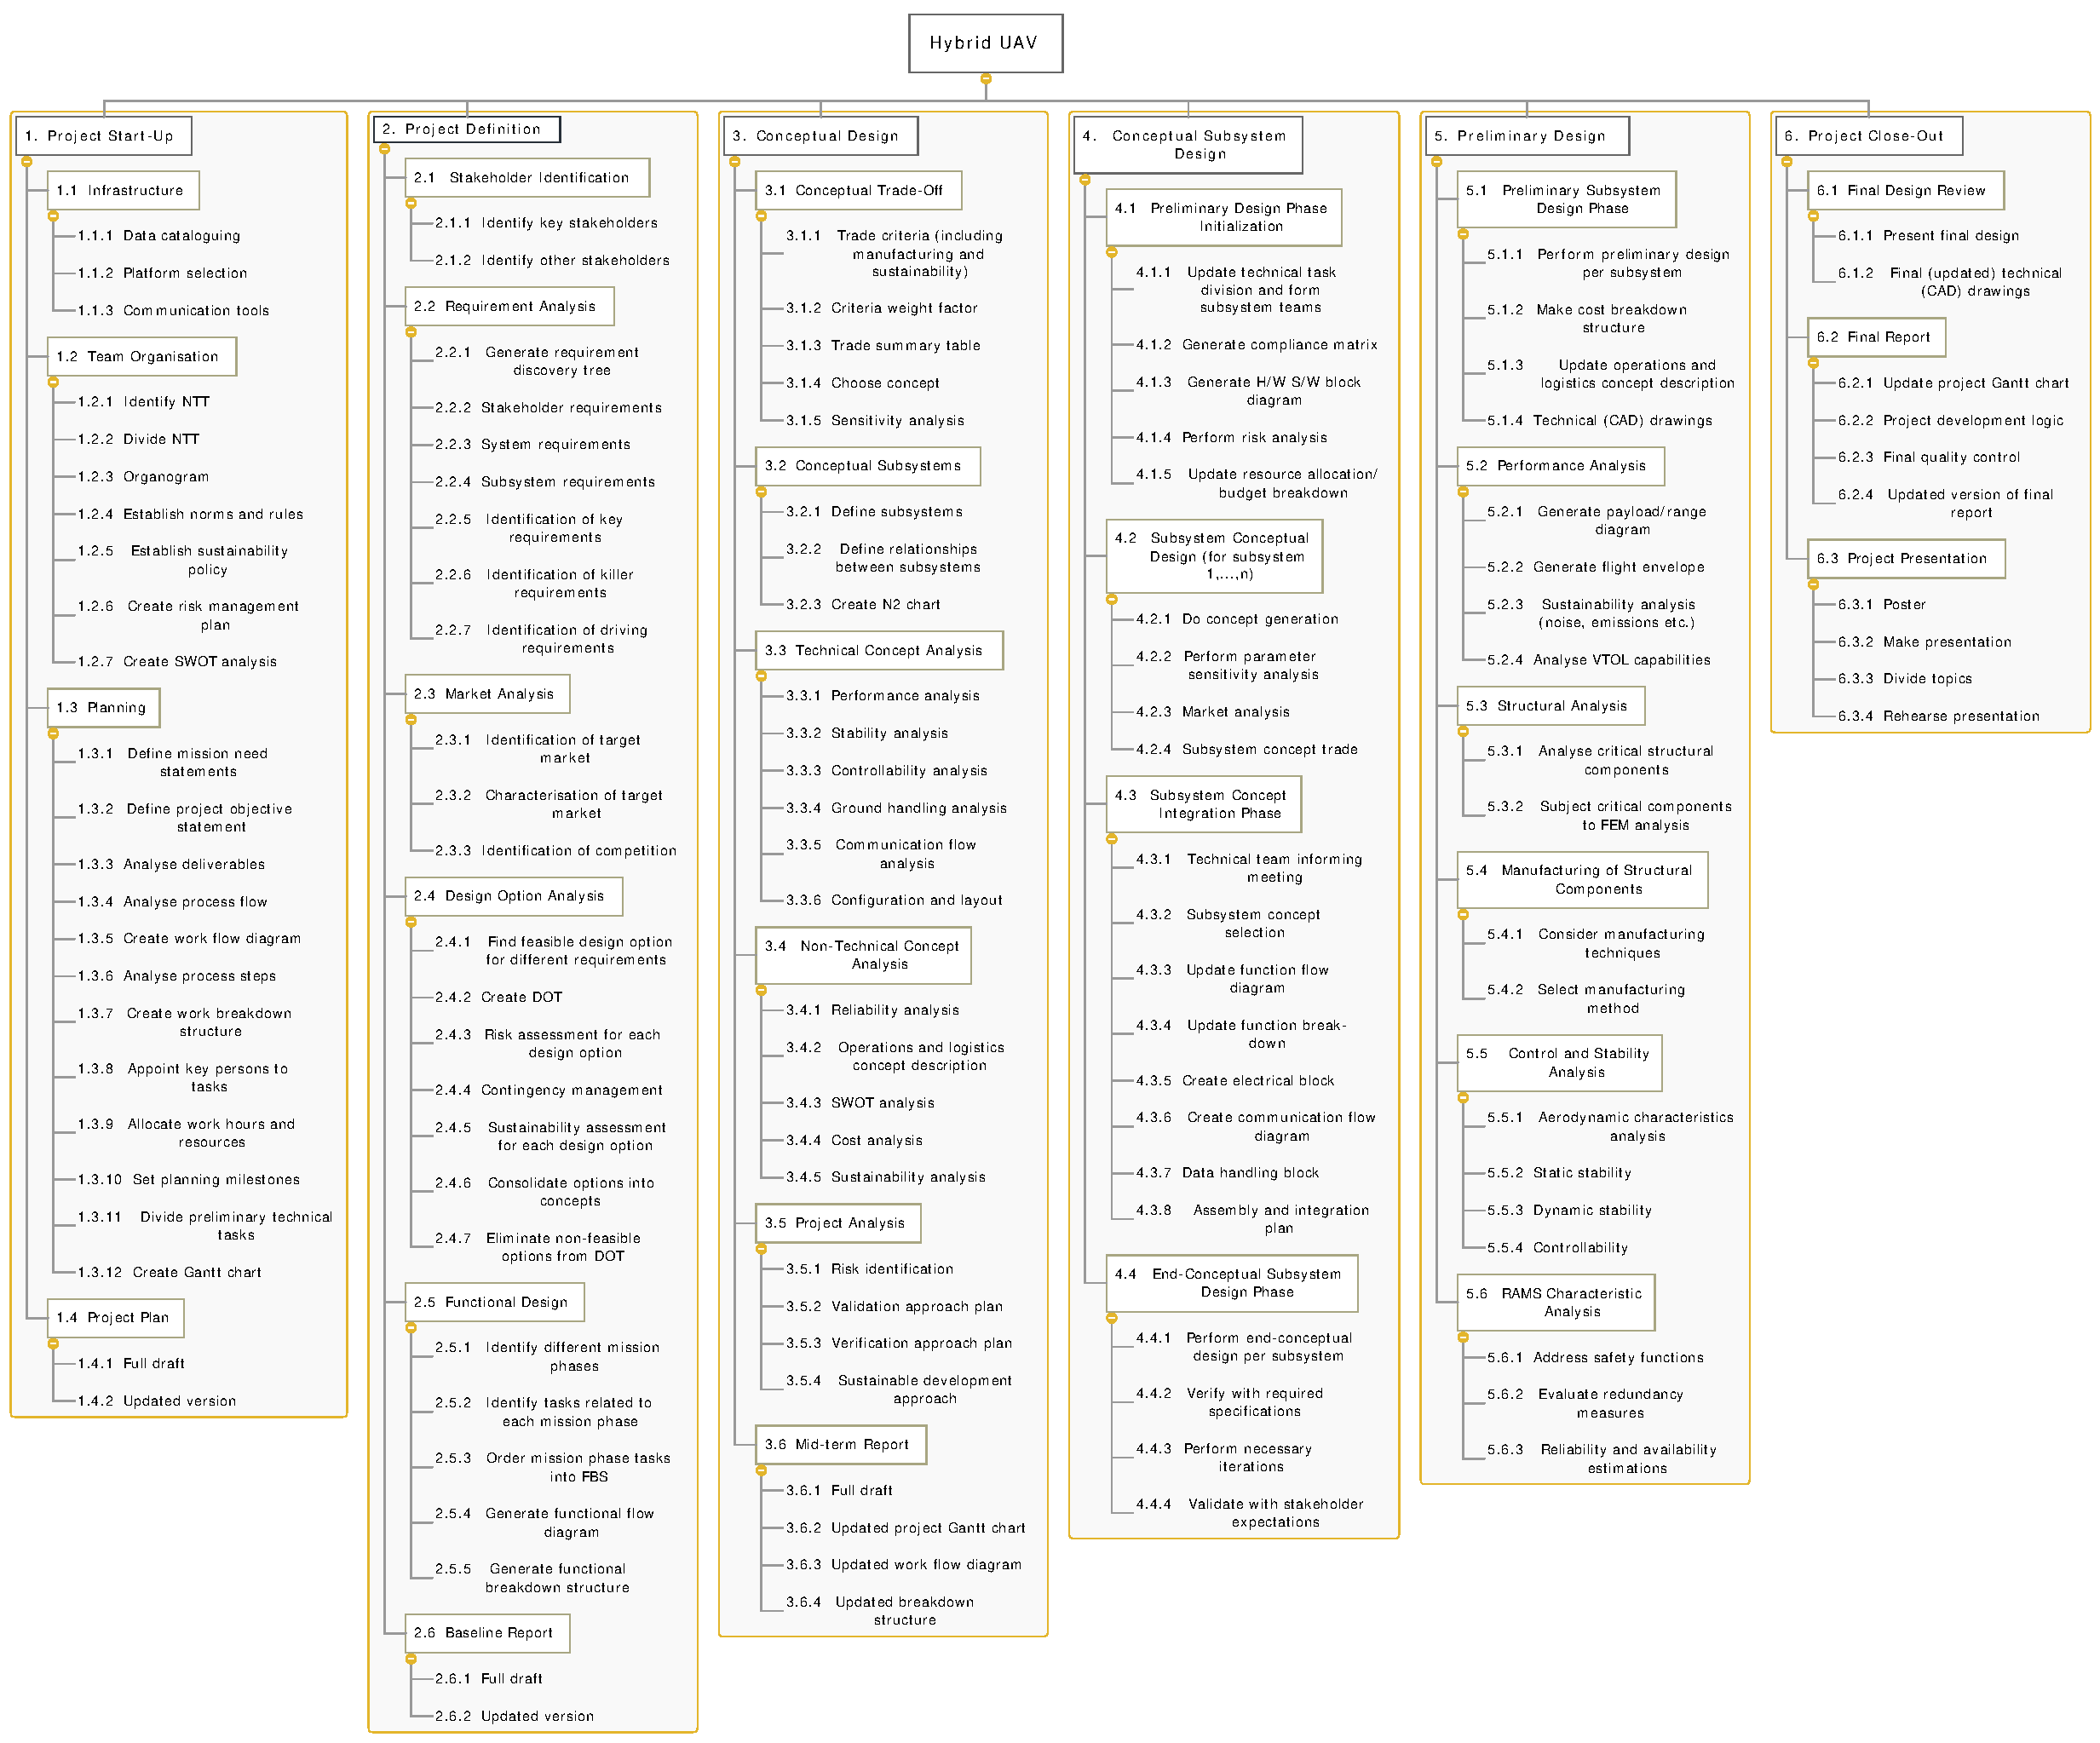
\includepdf[pages=1,fitpaper, scale=0.85,pagecommand={}]{ProjectOrganisation/Figures/WBS.pdf}

\newpage

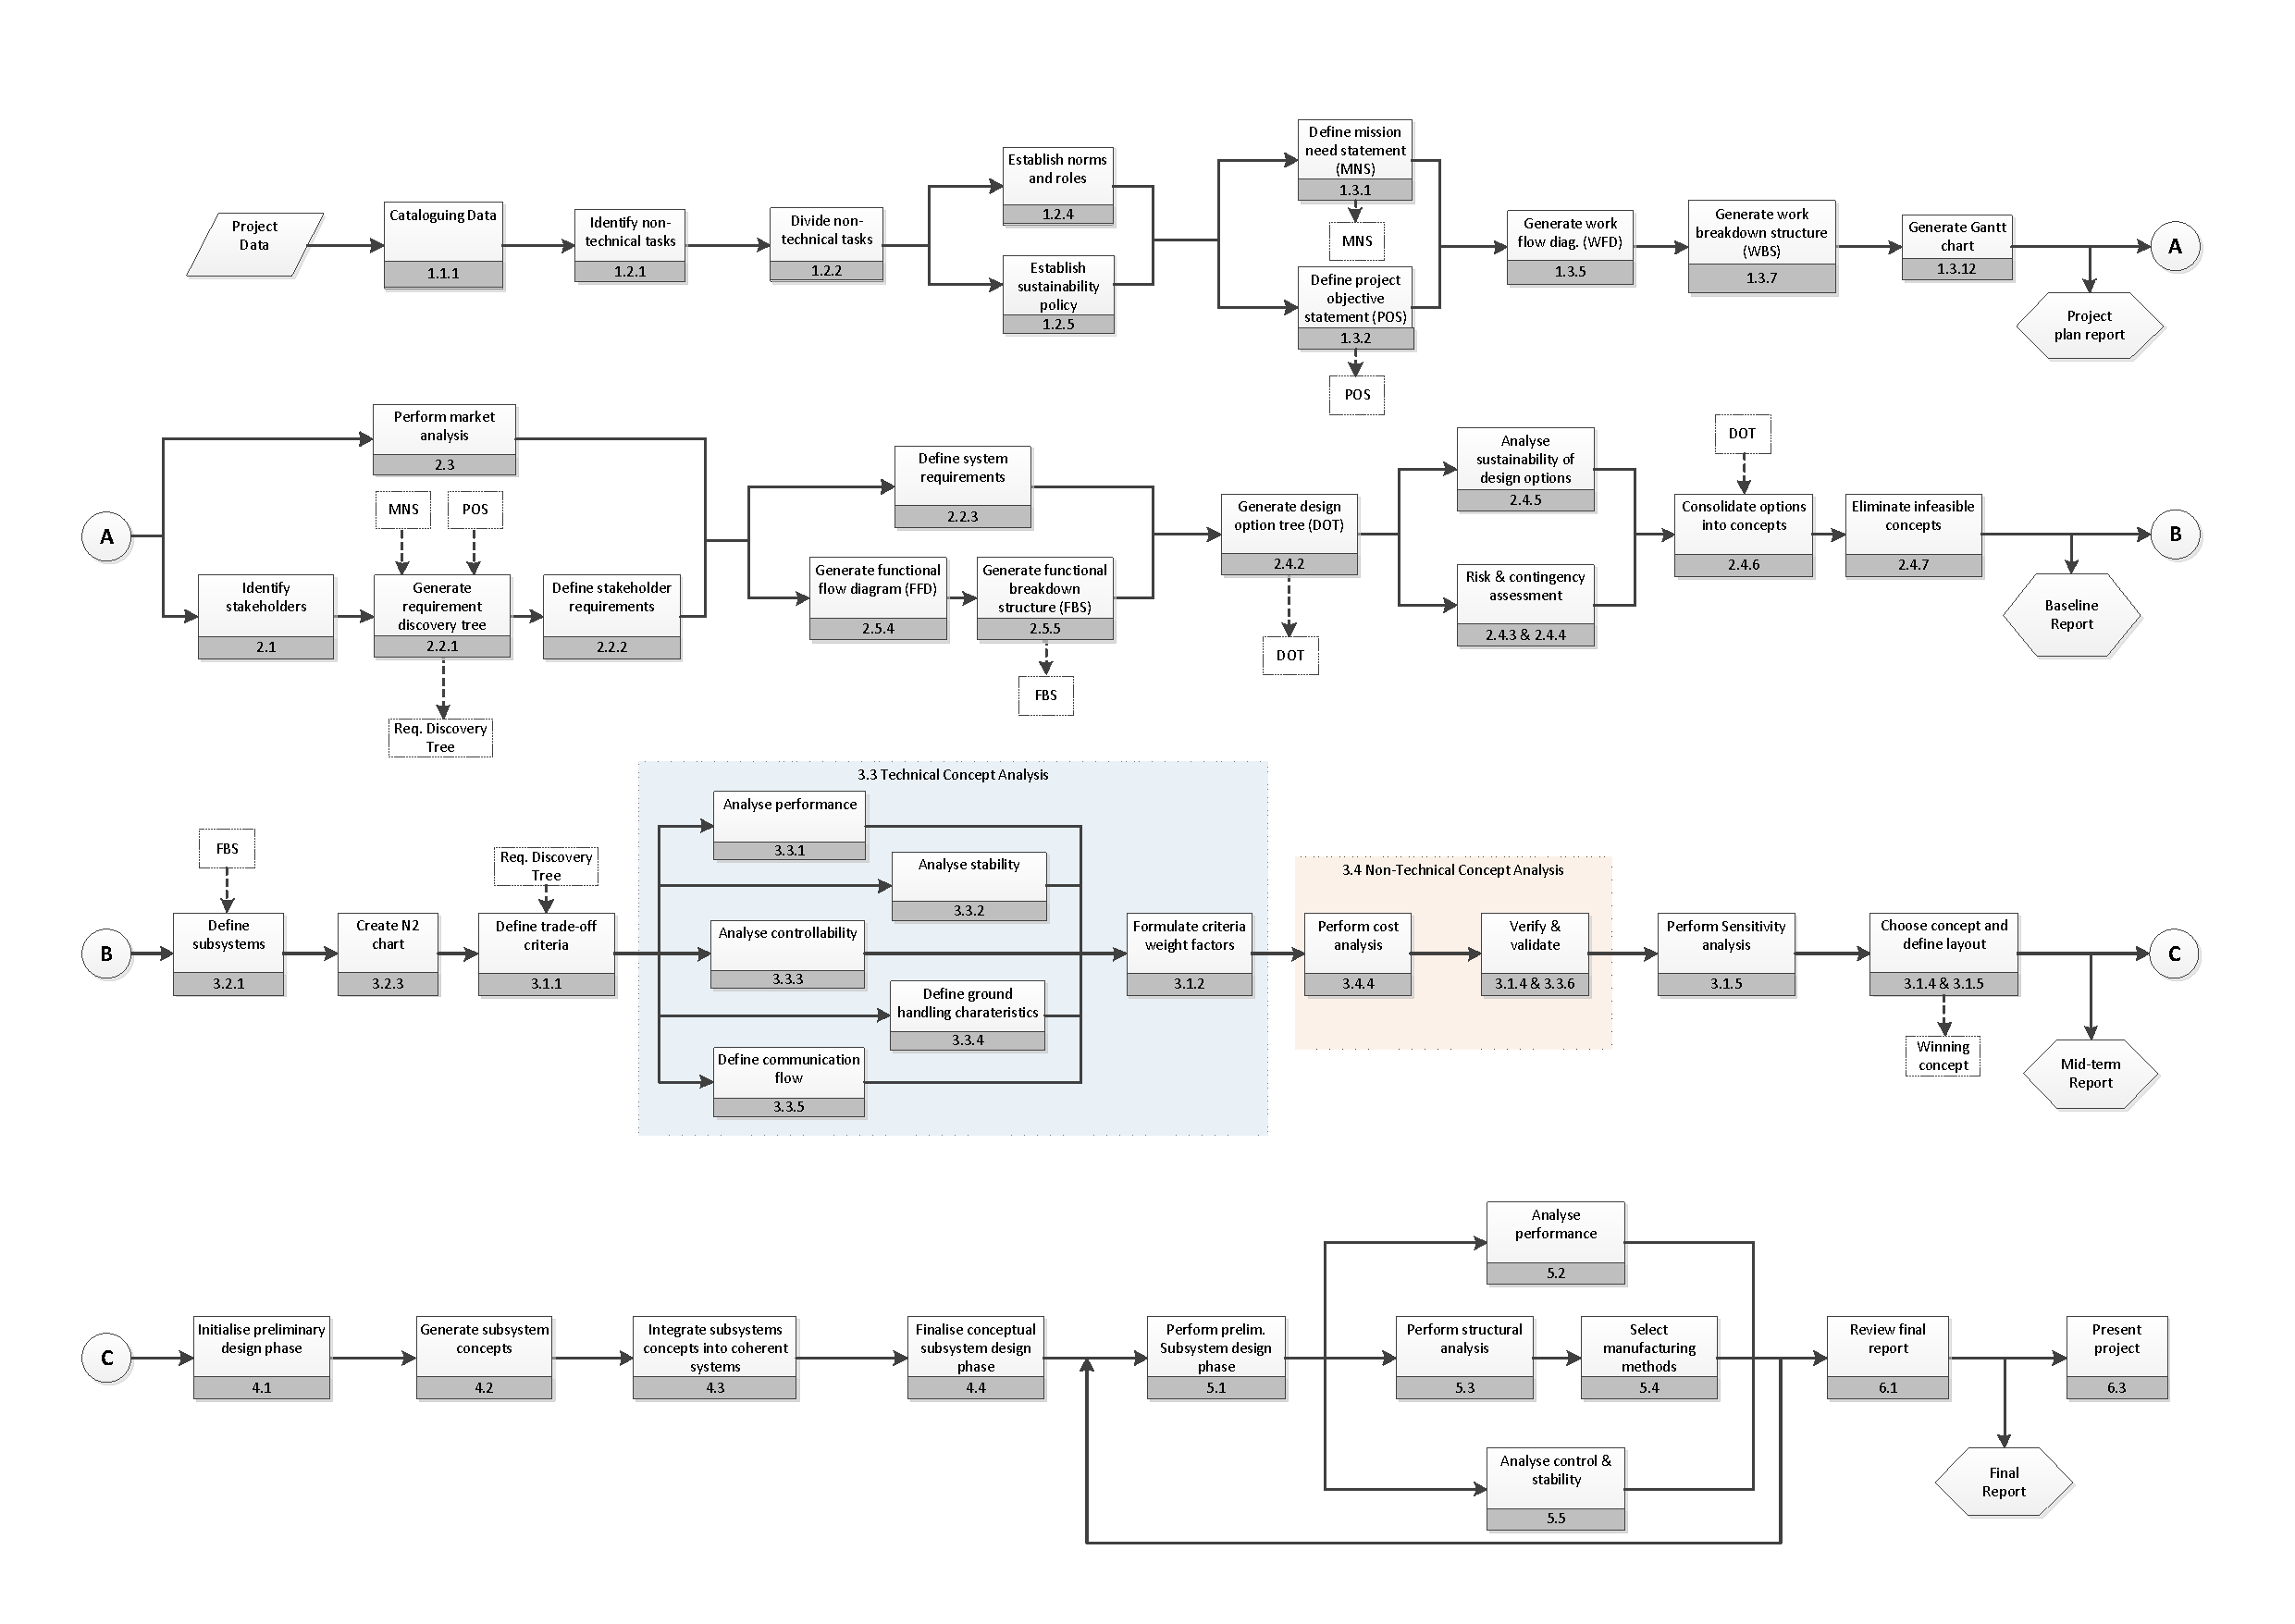
\includepdf[pages=1,fitpaper, scale=0.85,pagecommand={}]{ProjectOrganisation/Figures/WFD.pdf}

\newpage

%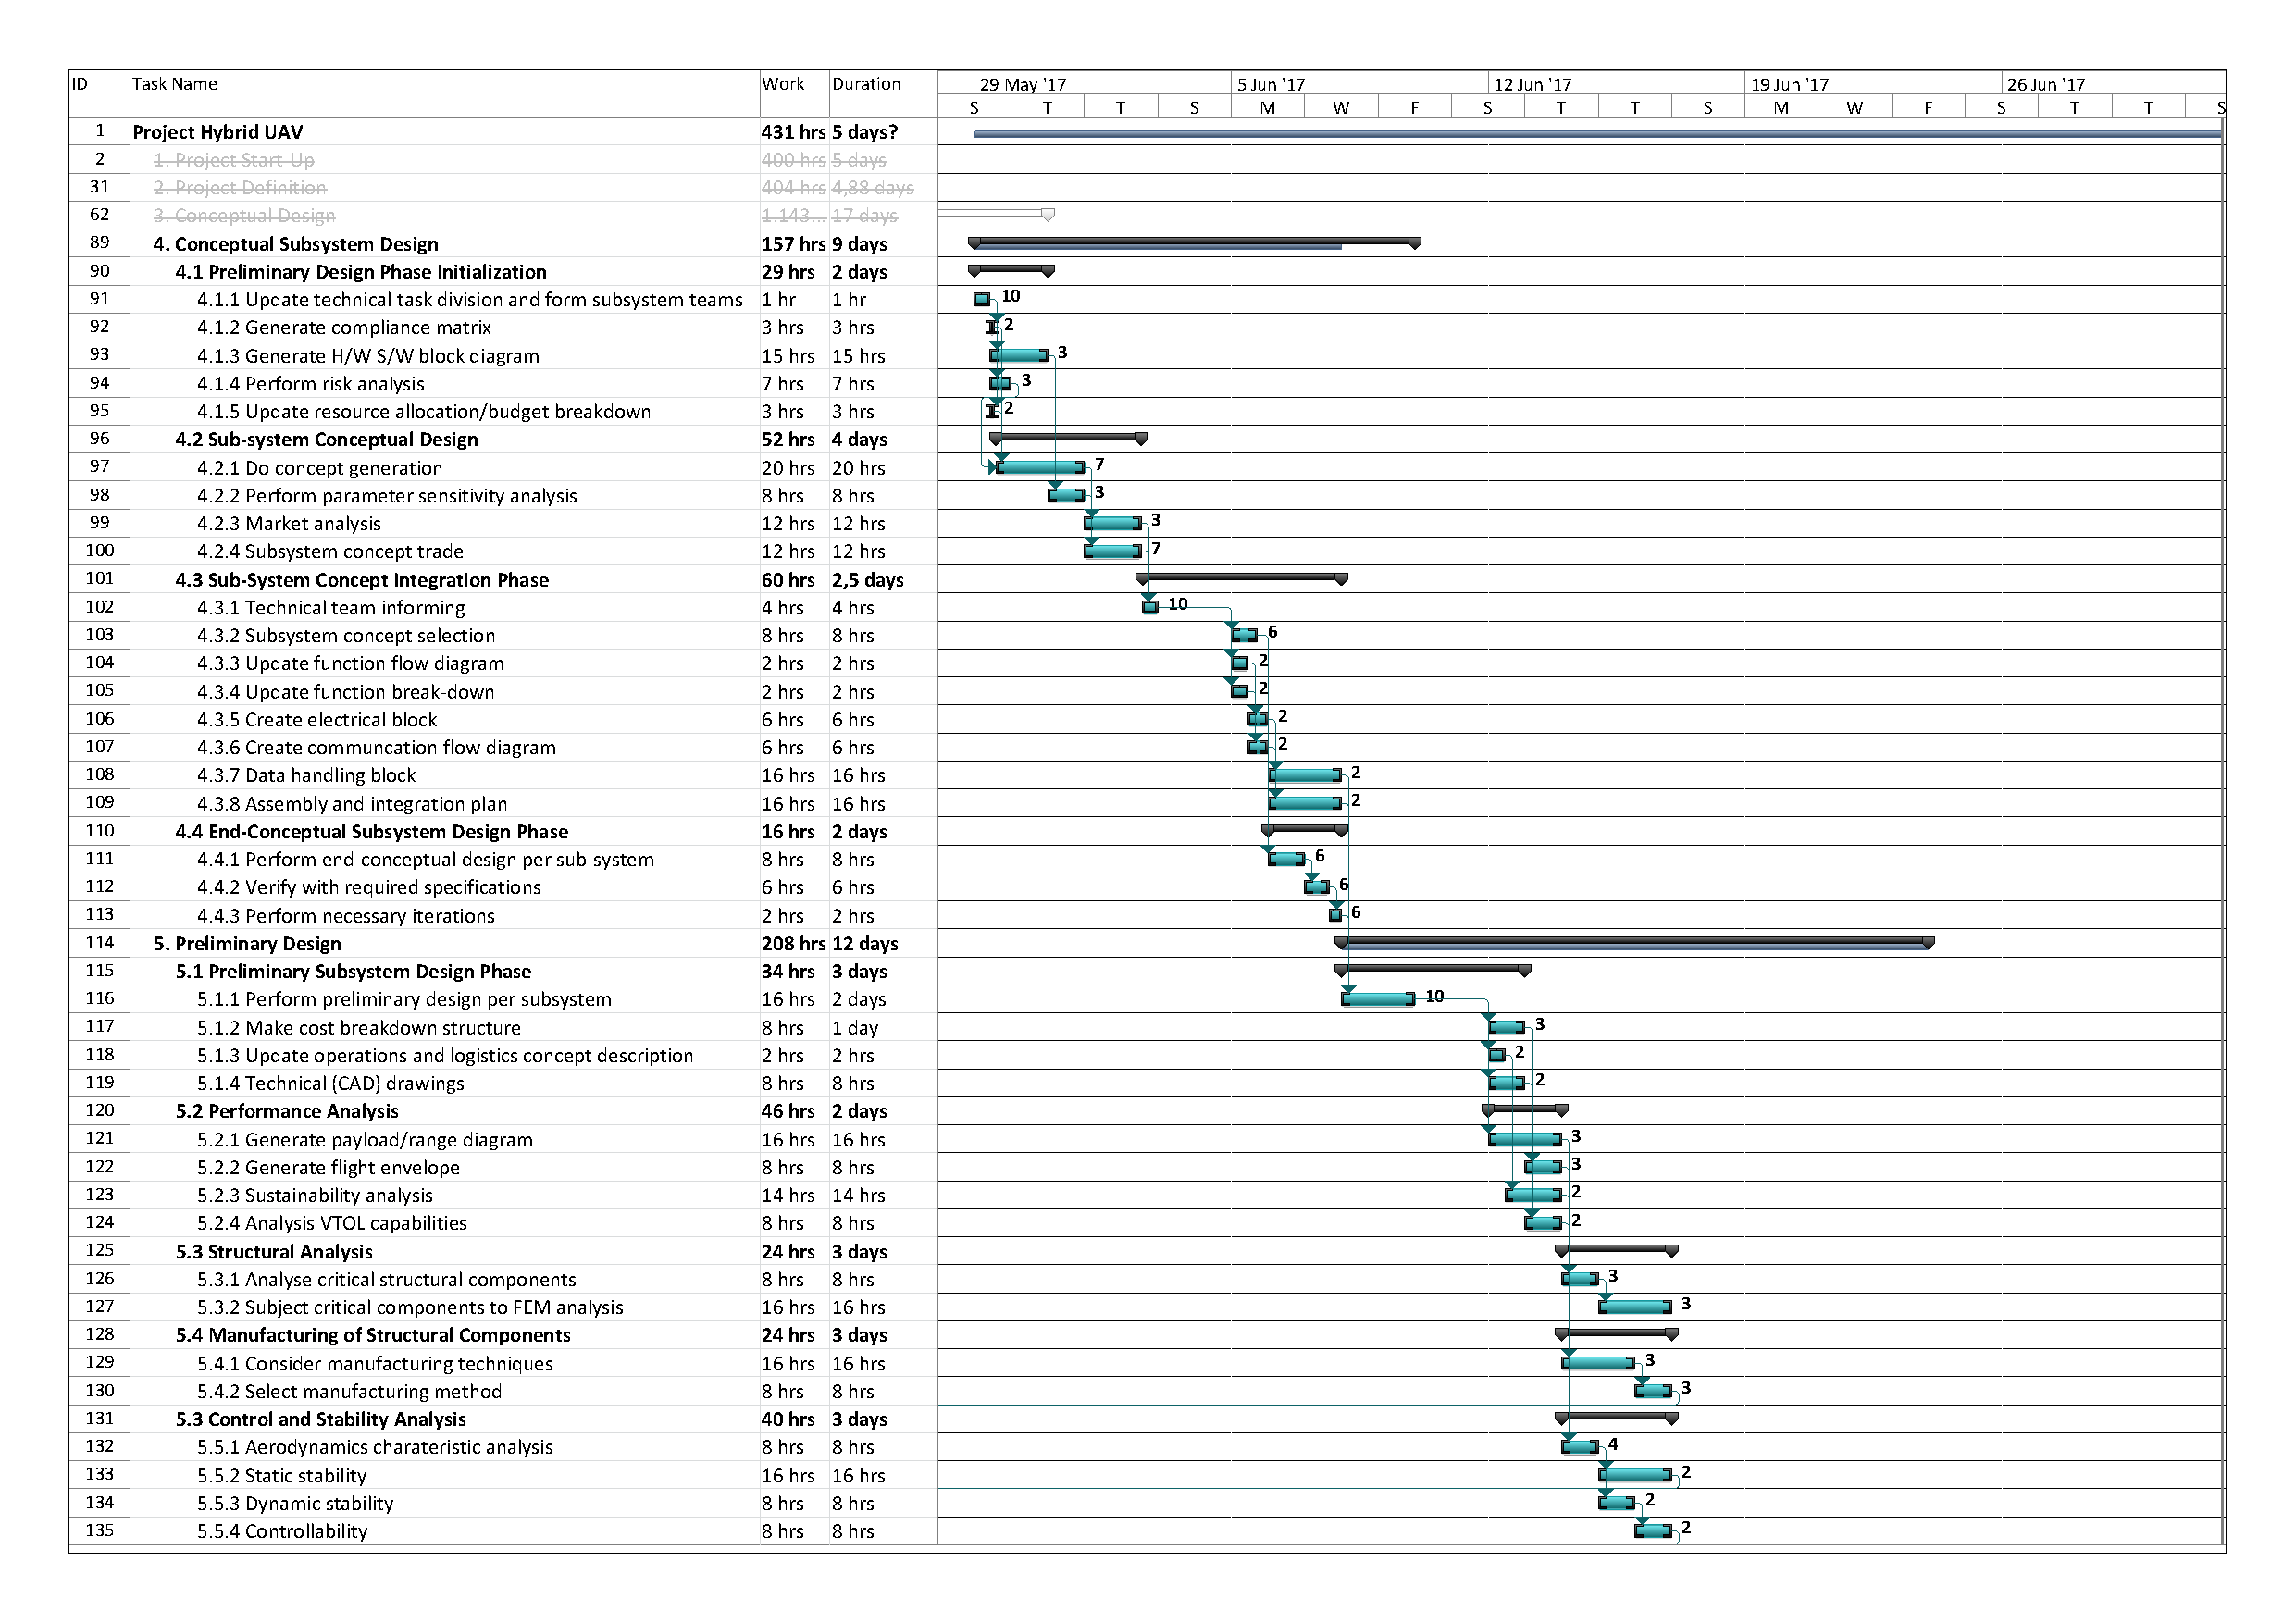
\includepdf[pages=1,fitpaper, scale=0.85,pagecommand={}]{ProjectOrganisation/Figures/Gantt_Final.pdf}

%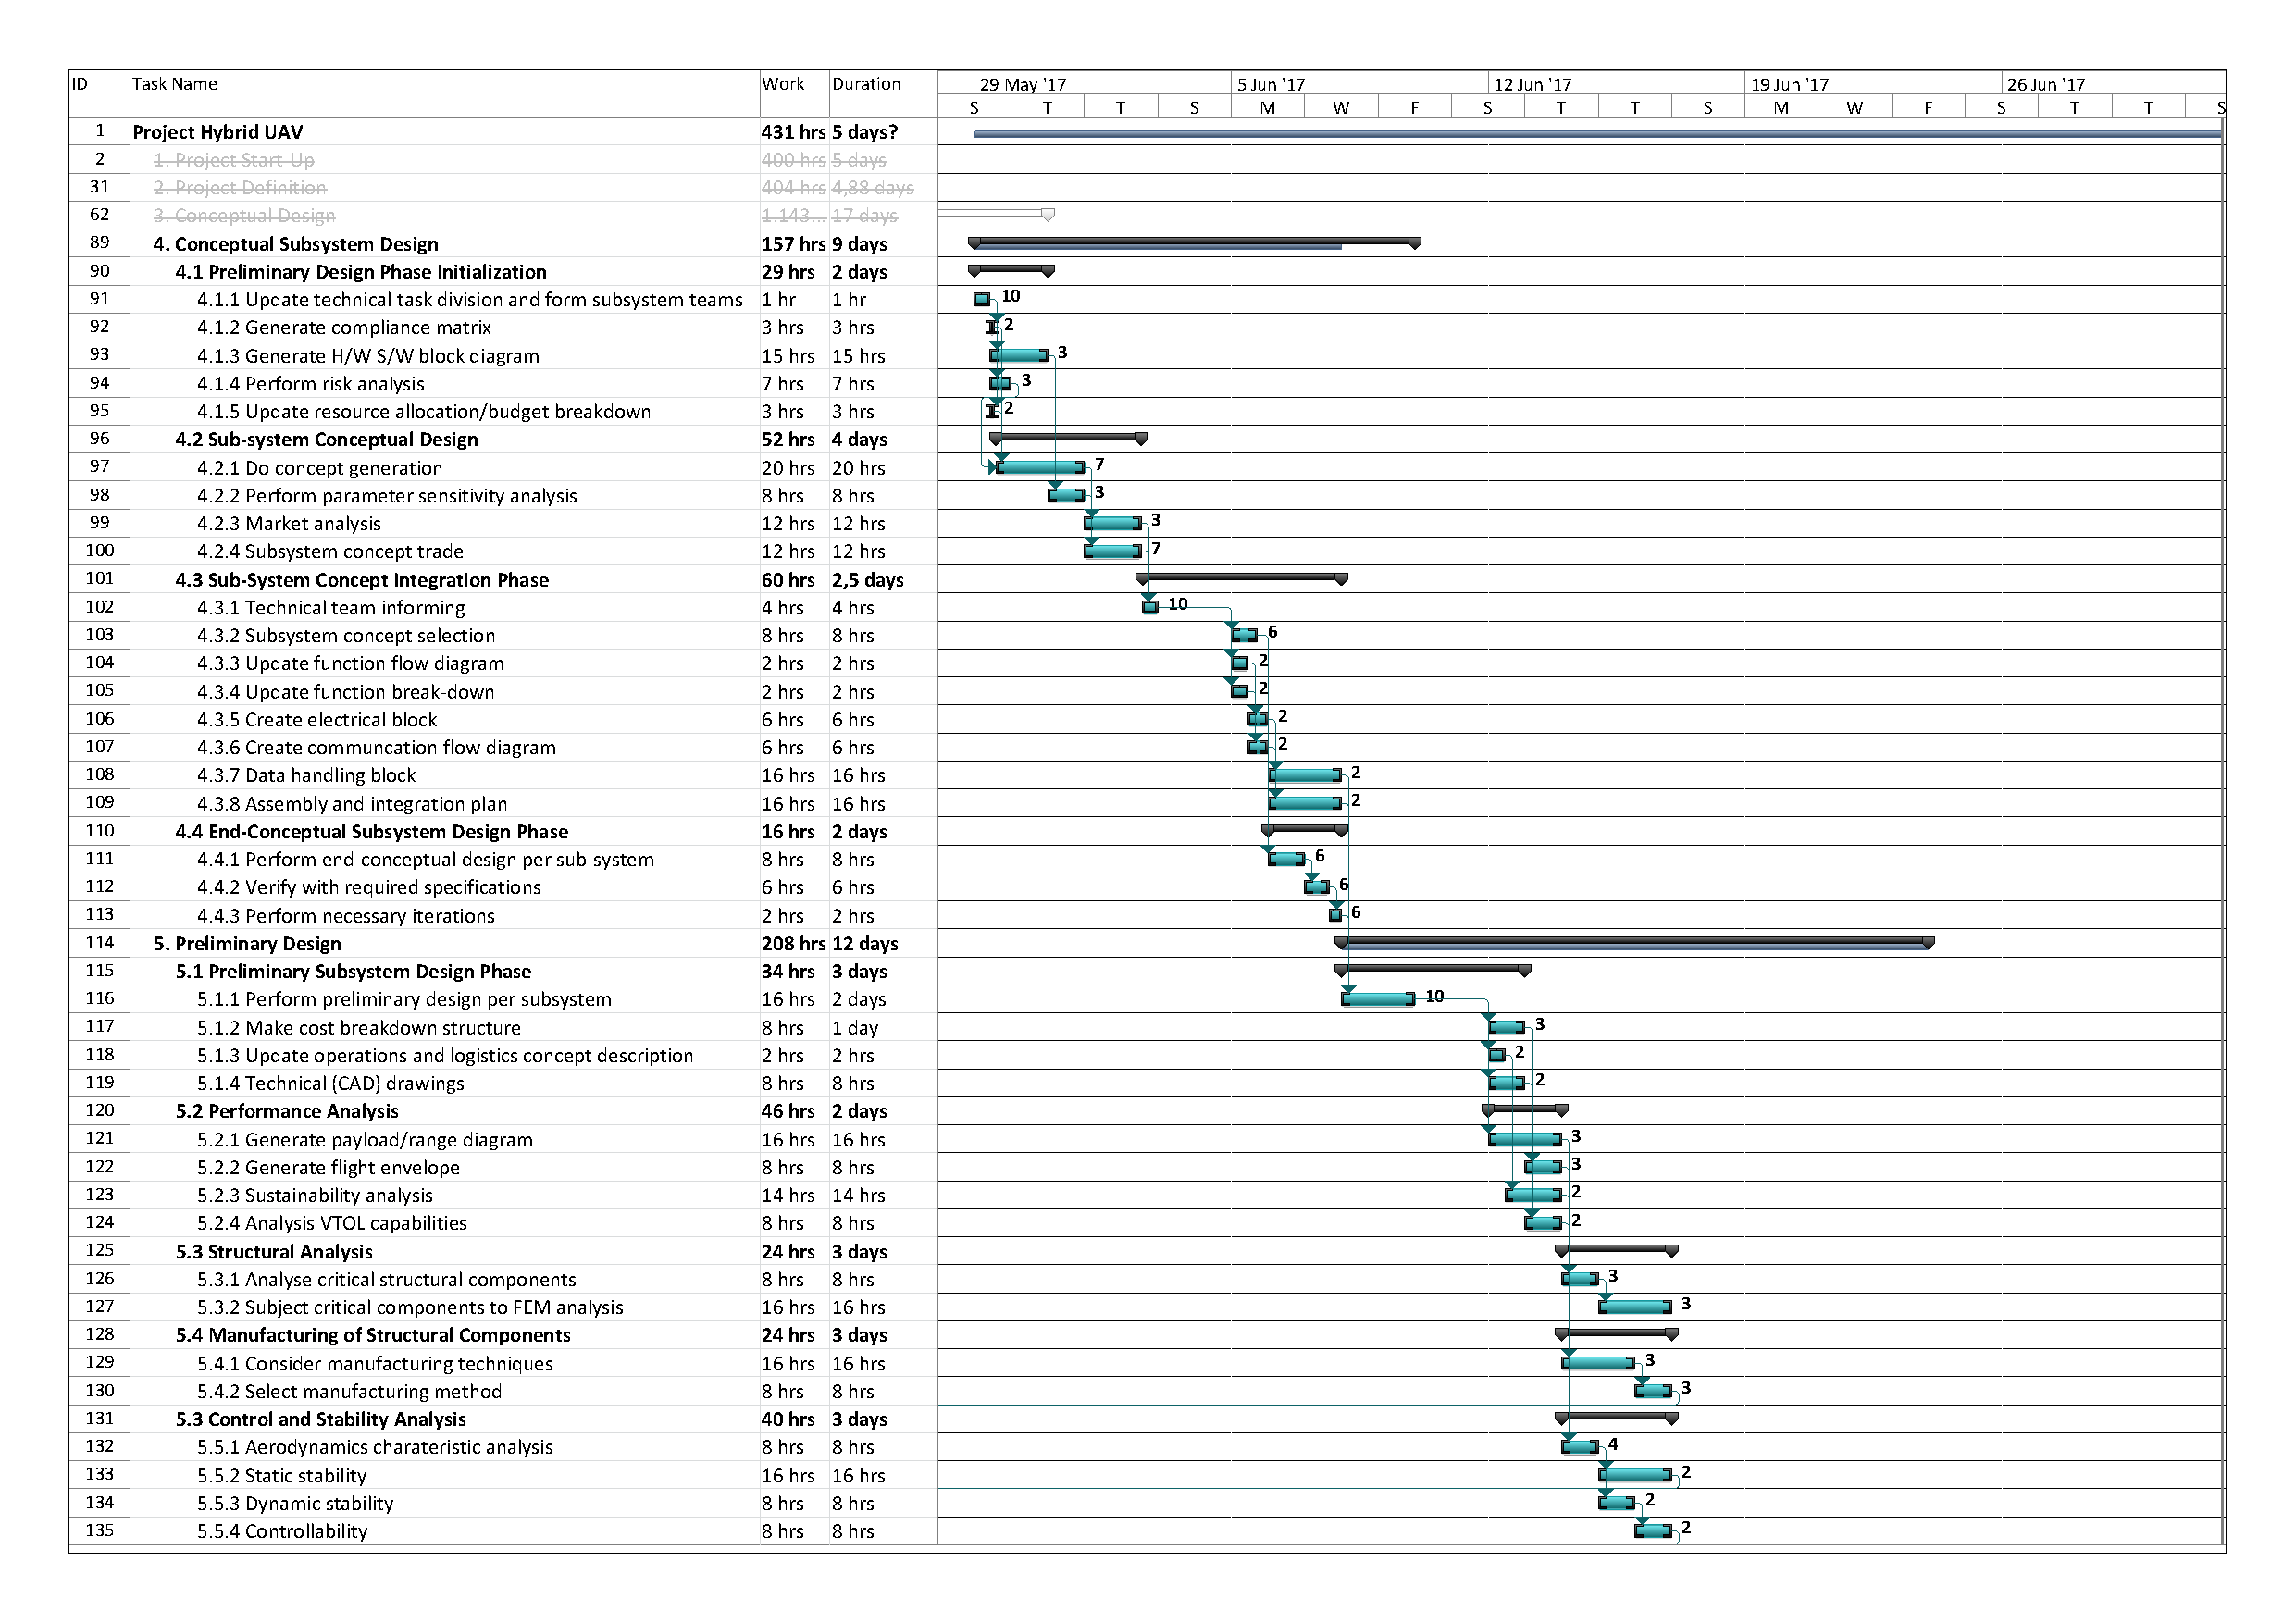
\includepdf[pages=1,fitpaper, scale=0.85,pagecommand={}]{ProjectOrganisation/Figures/Gantt_Final1.pdf}

%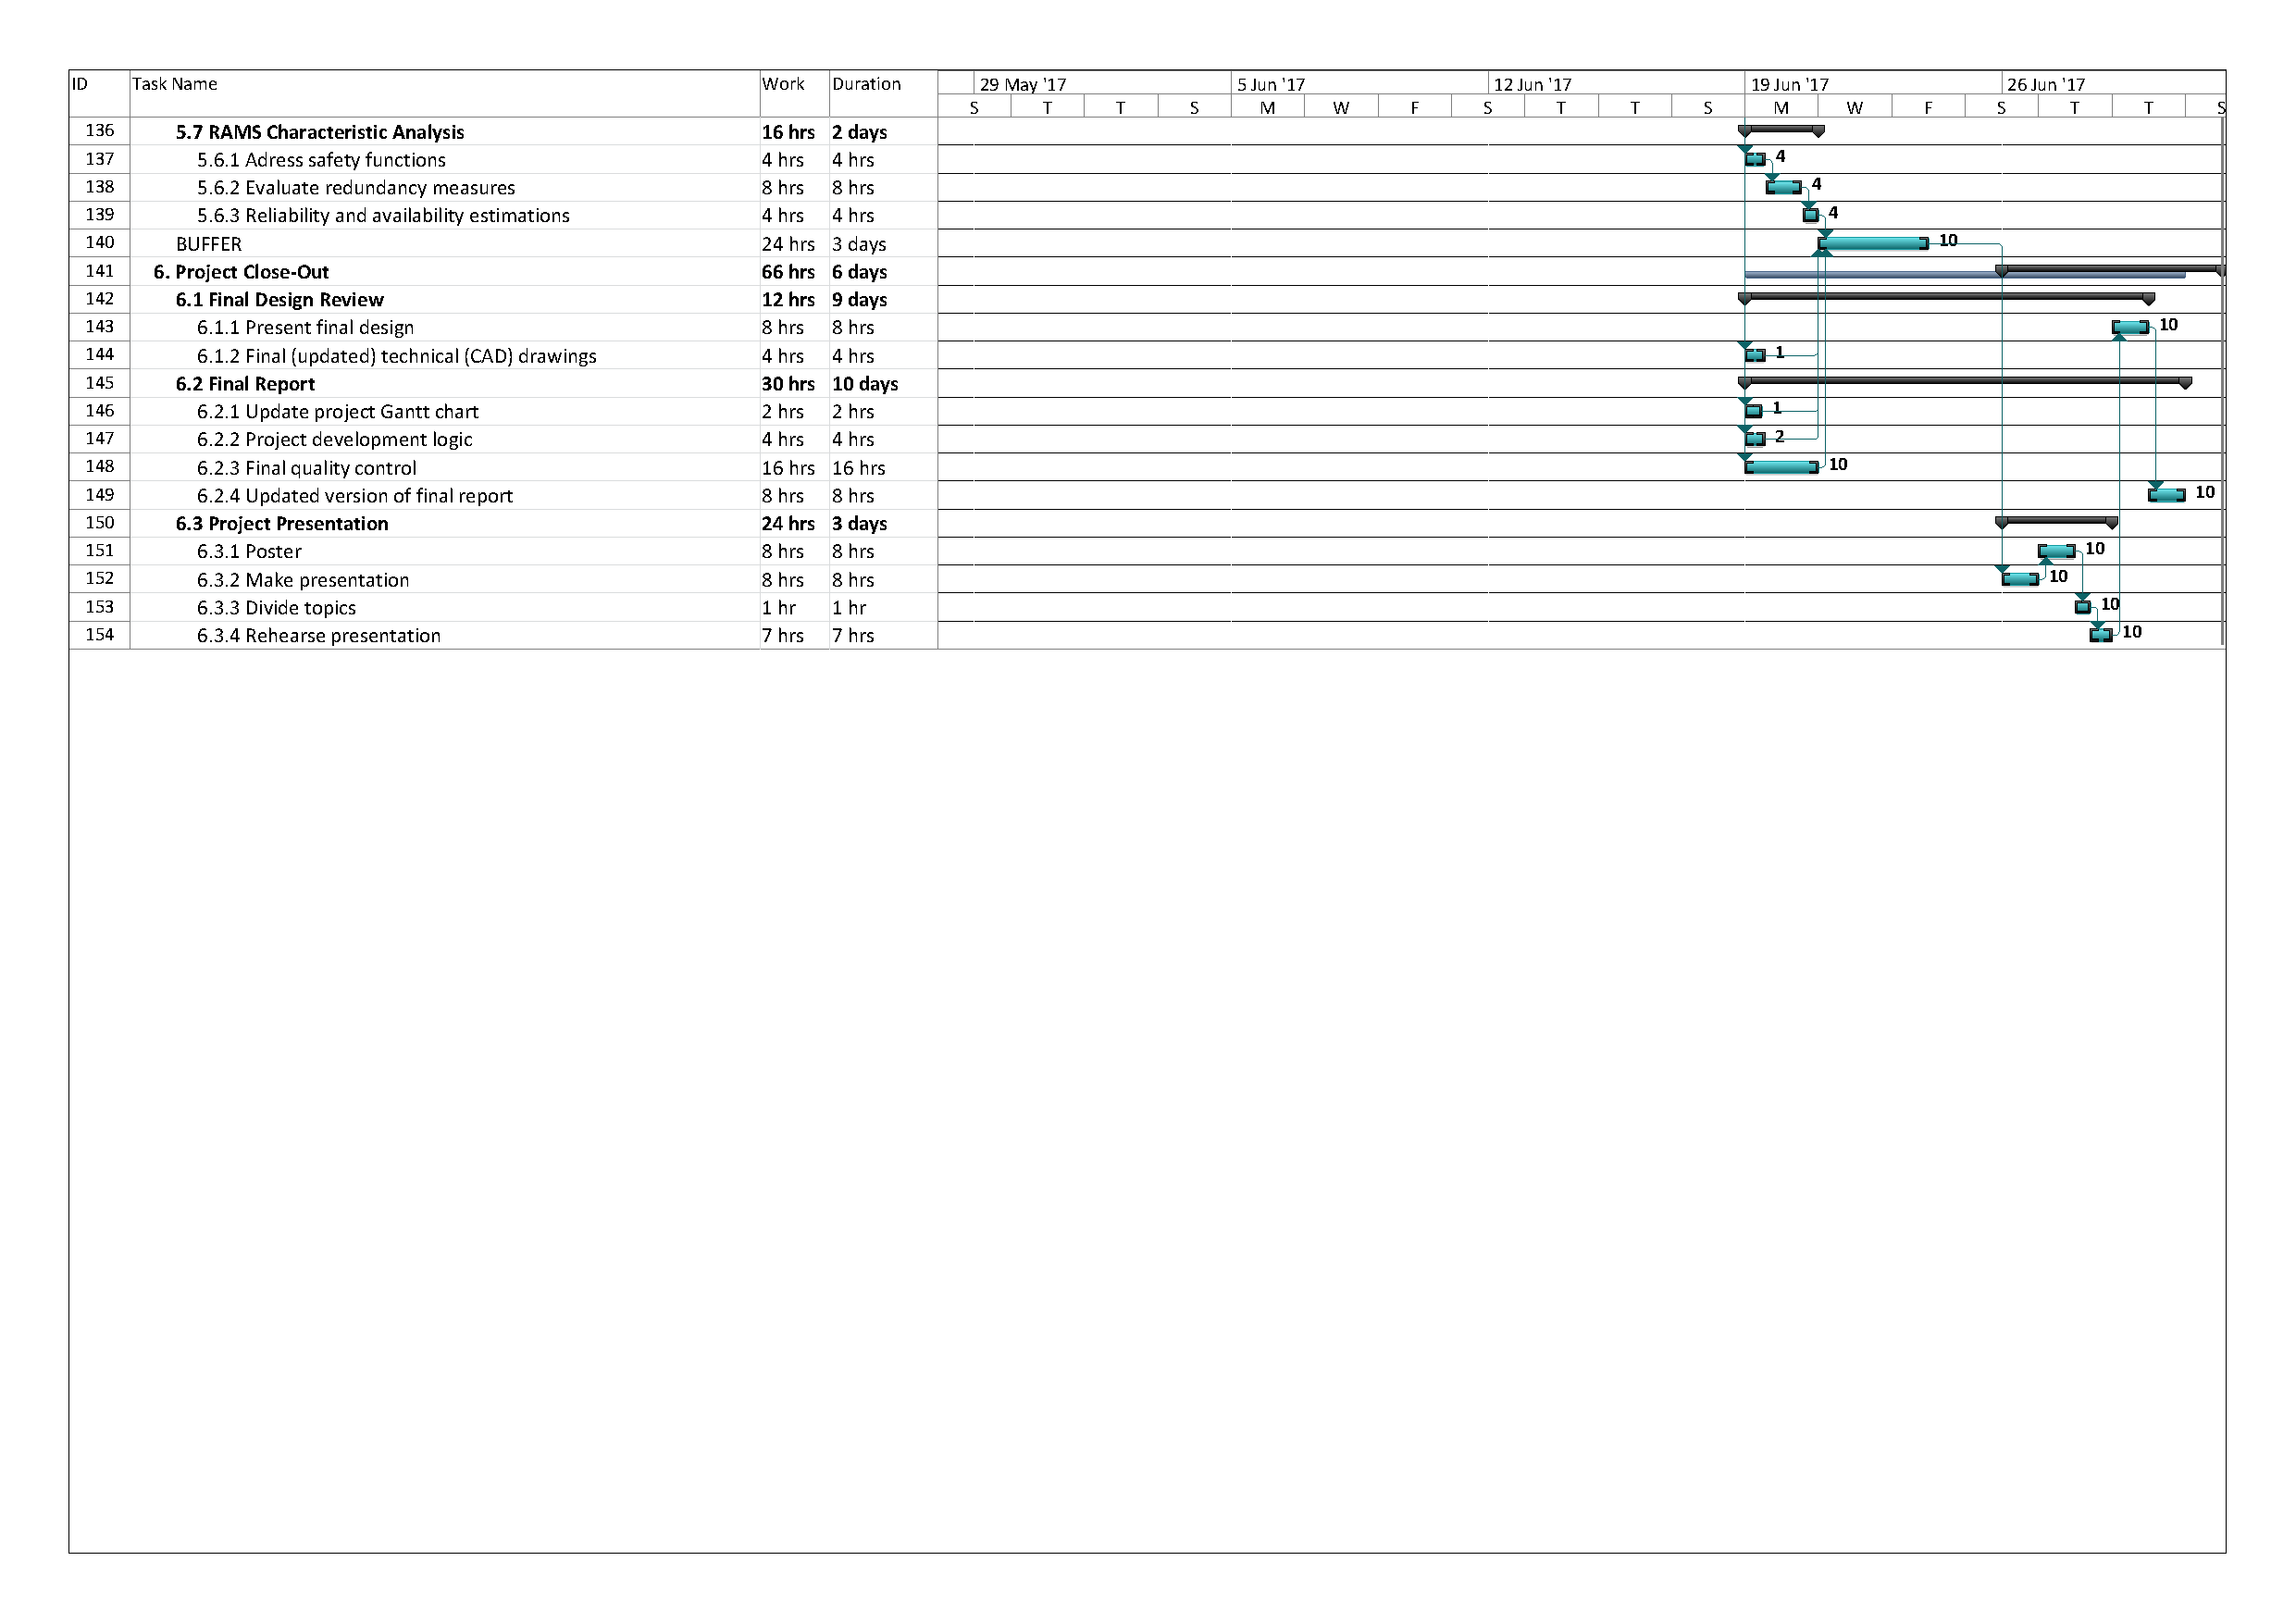
\includepdf[pages=1,fitpaper, scale=0.85,pagecommand={}]{ProjectOrganisation/Figures/Gantt_Final2.pdf}

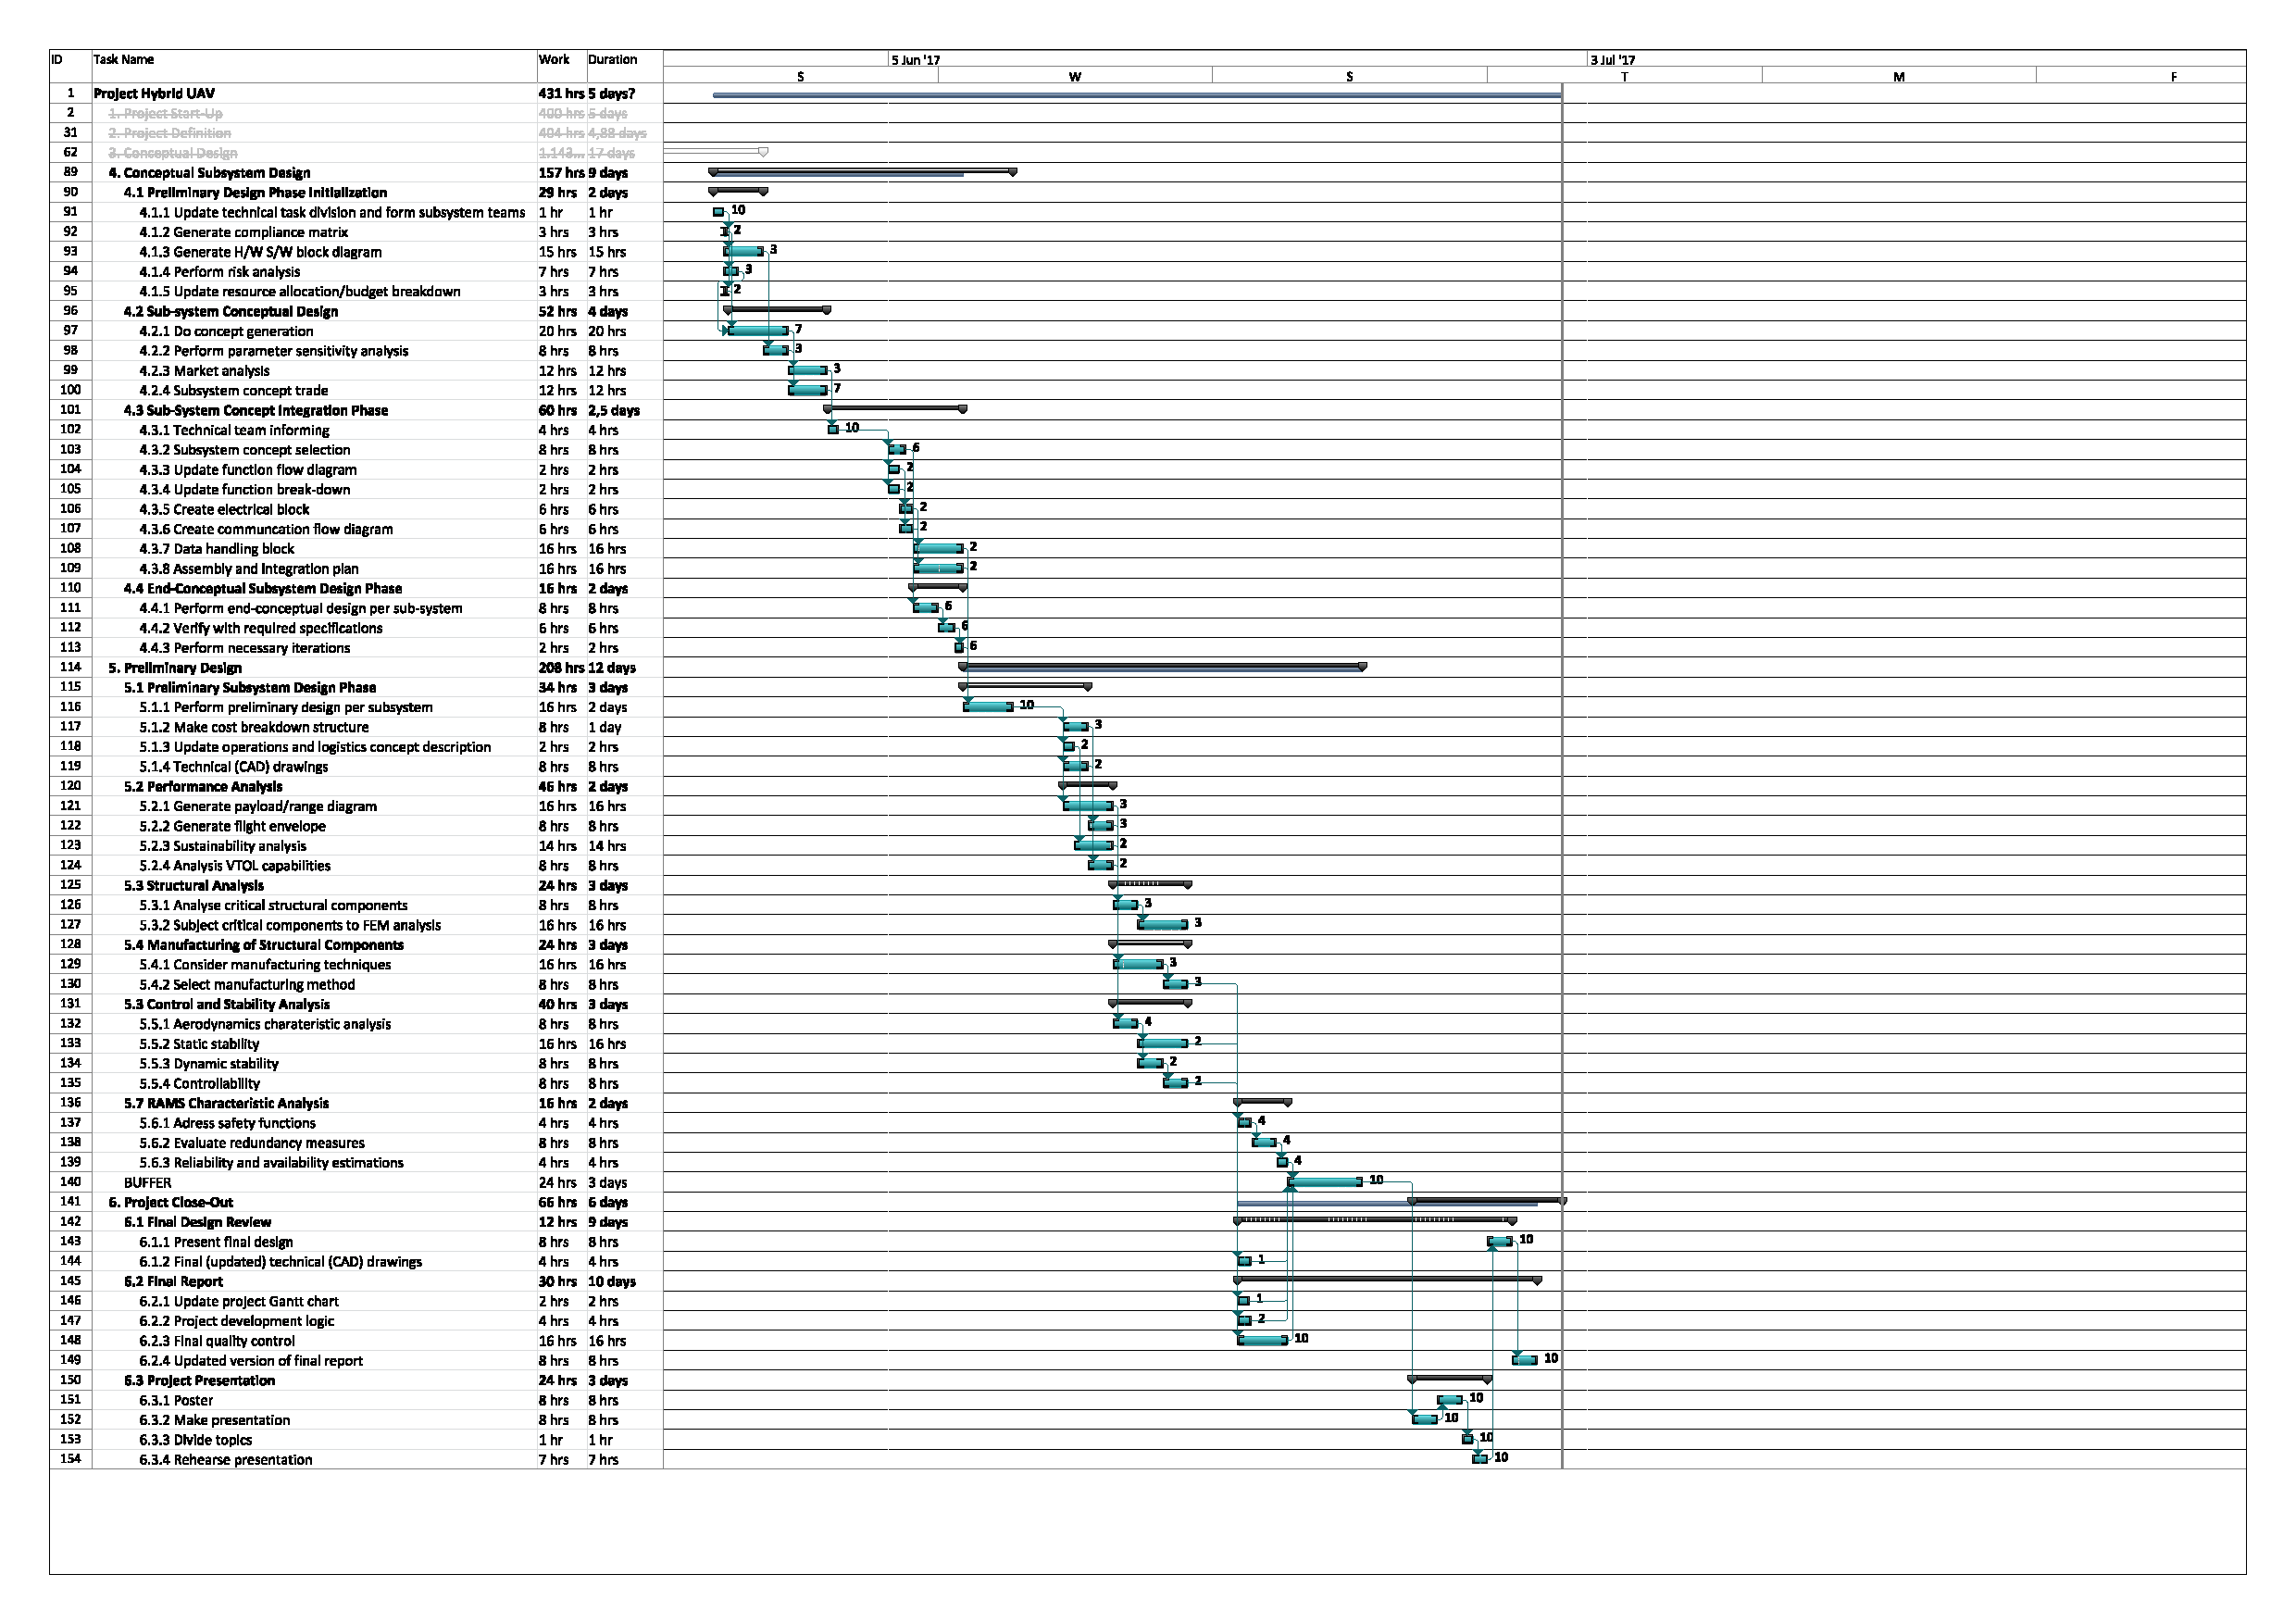
\includepdf[pages=1,fitpaper, scale=0.85,pagecommand={}]{ProjectOrganisation/Figures/gantt_small.pdf}
    \chapter{Revised Requirements}
\label{ch:requ}
\setlength{\parindent}{15pt}
%responsible persons: Joel and Piotr
%written by: Piotr and Joel
Defining requirements is crucial to development of any product, since these directly define or influence the design. They are of primary importance during the trade-off in the concept phase, since feasibility is assessed according to the requirements which they satisfy.

This chapter presents system requirements found at an earlier stage of the project. Since then, some requirements have been modified or removed. %The requirement coding may seem incomplete due to missing numbers, yet this indicates that previously defined requirements were removed from the list. 
The requirement coding is explained in \autoref{sec:lege} and the requirements are listed in \autoref{sec:requ}.  

\section{Legend}
\label{sec:lege}

\autoref{tab:lege} presents the legend explaining the meaning of the requirement coding.

\begin{table}[h]
\centering
\caption{Requirements Coding Legend}
\label{tab:lege}
\begin{tabular}{ll}
\toprule
\textbf{Requirement Code} & \textbf{Related to:}                       \\\midrule
SYS                       & System                                         \\\hdashline
C                         & Cost                                           \\\hdashline
S                         & Schedule                                       \\\hdashline
L                         & Legislation                                   \\\hdashline
R                         & Available resources                            \\\hdashline
ENV                       & Environmental conditions and footprint         \\\hdashline
PH                        & Physical characteristics                       \\\hdashline
OP                        & Operational performance                        \\\hdashline
PF                        & Flight performance                             \\\hdashline
VS                        & Vehicle systems                                \\\hdashline
*                         & Non-critical requirements (stakeholder wishes) \\\hdashline
\dag                      & Key requirements\tablefootnote{A requirement which is of primary importance for the customer.}                     \\\hdashline
\ddag                     & Driving requirements\tablefootnote{A requirement that drives that design more than average.}                 \\\hdashline
x                         & Killer requirements \tablefootnote{A requirement that drives the design to an unacceptable extent.}                 \\\bottomrule
\end{tabular}
\end{table}
%\addtocounter{footnote}{-2}
%\footnotetext{}
%\addtocounter{footnote}{1}
%\footnotetext{}
%\addtocounter{footnote}{1}
%\footnotetext{}

\section{Requirements}
\label{sec:requ}
The revised requirements are seen in the following list.

\begin{enumerate}[leftmargin =4.5cm, align=parleft, labelwidth=10em]
    \item[\textbf{SYS-C-1:} \dag \ddag] The production and distributed development cost per unit shall be limited to an amount of 30k Euros.
    \item[\textbf{SYS-C-2:}] The cost of the UAV support service shall not exceed 5k Euros per year.
    %\item[\textbf{SYS-C-3:}] The costs of disposal at end-of-life phase shall not  exceed 2.000 Euros.
    %\item[\textbf{SYS-S-1:}] The production time of one unit shall be limited to one month.
    \item[\textbf{SYS-S-2:}] The design (up to and including preliminary phase) of the UAV shall be done in 10 weeks.
    %\item[\textbf{SYS-L-1:}] The UAV shall conform with EASA regulations (Directive 2009/48/EC).
    \item[\textbf{SYS-L-2:} \dag] The UAV shall notify the operator when 120 m altitude is reached. 
    \item[\textbf{SYS-L-3:} x ] The UAV shall conform with EASA regulations (A3-Category).\footnote{EASA Regulations received through contact with AVY}
    \item[\textbf{SYS-R-1:}] The design shall be performed with not more than 10 team members.
   % \item[\textbf{SYS-RES-2:}] The design of the UAV shall be limited to components that are feasible to manufacture.
    %\item[\textbf{SYS-ENV-C:}] The UAV shall be able to operate under prior defined critical conditions.
    %\item[\textbf{SYS-ENV-1.1:} $\ast$ ] The UAV shall be able to operate in smoke with a visibility of 5m or more.
    %\item[\textbf{SYS-ENV-1.2:} $\ast$ ] The UAV shall be resistant to an exposure of elevated temperature up to 200 degrees Celsius for 20 minutes.
%    \item[\textbf{SYS-ENV-1.3:} $\ast$ ] The UAV shall be able to operate at rainfall of 7.6 mm of rain per hour (heavy rainfall).
    \item[\textbf{SYS-ENV-1.4:} $\ast$ ] The UAV shall be able to operate at wind conditions up to 6 on the Beaufort scale.
    \item[\textbf{SYS-ENV-1.5:}] The UAV shall have resistance against corrosion of safe-life components for its entire planned lifetime.
    \item[\textbf{SYS-ENV-1.6:} $\ast$ ] The UAV shall be able to operate nominally in temperatures ranging from -30 to +40 degrees Celsius.
    %\item[\textbf{SYS-ENV-1.7:} $\ast$ ] The UAV shall be able to endure storage temperatures ranging from +5 to +30 degrees Celsius.
    \item[\textbf{SYS-ENV-2.1:} \dag] The UAV shall not produce any carbon emissions during operation. 
    \item[\textbf{SYS-ENV-2.2:}] The UAV noise emission shall not exceed a limit of 68 dB.
    %\item[\textbf{SYS-ENV-2.3:}] The UAV shall not require any maintenance substances (i.e. paints, lubricants and anti-icing sprays) which are environmentally damaging and have an environmental impact neutral alternative.
    \item[\textbf{SYS-ENV-2.5:}] During production no substances harmful to the environment shall be used as prescribed by EU legislation.
    %\item[\textbf{SYS-ENV-2.6:}] The UAV's energy source shall be ENTER SOMETHING HERE!!!!!!!!!!!!!!!!!!!!!!!!!!!!!!!!!!!!!!!!!!!!!
%\item[\textbf{SYS-PH-1.1:}] The UAV shall have maximum dimensions of <tbd>.    
    \item[\textbf{SYS-PH-1.1:} \ddag] The combined UAV and support equipment shall occupy a maximum volume of 1.7 x 1.2 x 1.4 meters. 
    \item[\textbf{SYS-PH-1.2:} \dag] The UAV shall have a payload bay volume of 100 x 15 x 15 cm.    \item[\textbf{SYS-PH-2:} x ] The UAV shall not weigh more than 25 kg.
    %\item[\textbf{SYS-PH-2:}] The UAV shall not weigh more than 150 kg.
    %\item[\textbf{SYS-PH-3:}] The UAV shall have an appearance that satisfies the customer's preferences. 
    %\item[\textbf{SYS-PH-4.1:}] The UAV shall not fail under the loads generated under normal operating conditions.
    %\item[\textbf{SYS-PH-4.2:}] The UAV structure shall not enter into resonance under the influence of the propulsion system.
    \item[\textbf{SYS-PH-4.3:}] The UAV shall have no single point of failure.
    \item[\textbf{SYS-PH-4.4:}] The UAV shall sustain accelerations from -1g up to +3g’s.

%\item[\textbf{SYS-OP-1.1:}] The UAV shall facilitate the payload with conditions to perform its mission.
%    \item[\textbf{SYS-OP-PB-1.1}:] The UAV shall be able to carry supplies.
    \item[\textbf{SYS-OP-1.1:}] The UAV shall be able to airdrop its payload during operation.
%    \item[\textbf{SYS-OP-1.1.2:}] The UAV shall be able to carry an organ transplant package of 10 kg maximum.
    %\item[\textbf{SYS-OP-1.2:}] The UAV shall not damage the payload under normal operating conditions.
    %\item[\textbf{SYS-OP-1.3:} $\ast$ ] The internal temperature of the UAV's payload bay shall not exceed 30 degrees Celsius under normal operating conditions. 
 %   \item[\textbf{SYS-OP-1.4:}] The UAV payload bay shall have universal and specific attachment systems for different types of payload.
   % \item[\textbf{SYS-OP-1.4:} $\ast$ ] The payload bay shall provide protection from external conditions.
    \item[\textbf{SYS-OP-1.5:} $\ast$ ] The payload bay shall provide a connection to the power storage.
    %\item[\textbf{SYS-OP-1.6.1:}] The payload bay shall limit the vibrations exerted on the payload to frequencies ranging from <tbd> to <tbd> Hertz. 
    %\item[\textbf{SYS-OP-1.6.2}] The payload bay shall limit vibrations exerted on the payload to a maximum amplitude of 1 mm.
    \item[\textbf{SYS-OP-1.7:} $\ast$ ] The UAV payload bay shall allow for payload mounting with basic tooling.
    %\item[\textbf{SYS-OP-1.8:}] The UAV payload bay shall ensure that the payload does not damage the UAV under normal operating conditions.
    
    \item[\textbf{SYS-OP-2.1:}] The UAV shall have an operational life of at least 1500 flying hours.
    %\item[\textbf{SYS-OP-2.2:}] The UAV system shall ensure sustainable disposability as dictated by <section in the baseline report>.
    \item[\textbf{SYS-OP-2.2:}] The UAV shall perform missions with a reliability of at least 75\%.
    \item[\textbf{SYS-OP-2.3:} ] The UAV shall be constructed with off-the-shelf electrical components.
    \item[\textbf{SYS-OP-2.4:} $\ast$ ] UAV fail-safe components shall not require specialised skills to be replaced.
    %\item[\textbf{SYS-OP-2.6:}] The UAV shall not cause any damage.
    %\item[\textbf{SYS-OP-2.5.1:}] The UAV shall be able to avoid collisions with other objects autonomously.
    %\item[\textbf{SYS-OP-2.5.2:}] The UAV shall contain an equivalent to an ADS-B safety communication system.
    \item[\textbf{SYS-OP-2.5.3:}] The UAV shall avoid collisions with other aircraft autonomously.
    \item[\textbf{SYS-OP-2.5.4:}] The UAV shall be able to avoid collisions with birds autonomously.
    \item[\textbf{SYS-OP-2.5.5:}] The UAV shall avoid collisions with ground objects autonomously.
    %\item[\textbf{SYS-OP-2.7}:] The UAV shall have an assembly time of less than 15 minutes.
    %\item[\textbf{SYS-OP-2.8}:] The assembly of the UAV shall not require specialised skills.
    %\item[\textbf{SYS-OP-2.6:} $\ast$ ] The UAV energy source shall be accessible using off-the-shelf tooling.
    \item[\textbf{SYS-OP-2.7:}] The UAV shall be able to operate in night conditions.
    %\item[\textbf{SYS-OP-2.8.1:} $\ast$ ] The UAV shall have a energy source that can be replaced within 5 minutes with off-the-shelf tooling.
    \item[\textbf{SYS-OP-2.8.2:} $\ast$ ] The UAV shall have a maximum turnaround time of 20 minutes.
    %\item[\textbf{SYS-OP-2.8.3:} $\ast$ ] The UAV pre-flight preparations shall be performed one person.
    %\item[\textbf{SYS-OP-2.8.4:} $\ast$ ] The UAV pre-flight preparations shall not require special skills.
    %\item[\textbf{SYS-OP-2.8.5:} $\ast$ ] The UAV post-flight inspection shall be performed by one person.
    \item[\textbf{SYS-OP-2.8.6:} $\ast$ ] The transport of the UAV shall require two persons.
    \item[\textbf{SYS-OP-2.8.7:} $\ast$ ] The in-flight operation of the UAV shall be performed by one person.
    \item[\textbf{SYS-OP-2.8.8:} $\ast$ ] The UAV energy source shall be replaceable within 5 minutes.
    %\item[\textbf{SYS-OP-2.8.9:} $\ast$ ] The UAV shall have an energy source that can be replaced with off-the-shelf tooling.
    %\item[\textbf{SYS-OP-2.9.1:}] The UAV shall have an installed operational safe-mode.
    \item[\textbf{SYS-OP-2.9.2:}] The safe mode of the UAV shall have a return-to-base function.
    \item[\textbf{SYS-OP-2.9.3:}] The safe mode of the UAV shall contain an autonomous emergency landing function.
    \item[\textbf{SYS-OP-2.9.4:}] The safe mode of the UAV shall be able to send a distress signal to the UAV operator, in case of an emergency.
    \item[\textbf{SYS-PF-1.1:} \ddag] The UAV shall be able to carry a payload of at least 10 kg.
	\item[\textbf{SYS-PF-1.2:} \ddag] The UAV shall be able to fly at a horizontal velocity of at least 200 km/h at cruise altitude carrying 10kg of payload.
	\item[\textbf{SYS-PF-1.3:} \dag] The UAV shall have a minimum range of 200 km carrying 10kg of payload.
	\item[\textbf{SYS-PF-1.4:}] The UAV shall have a minimum endurance of 1 hour carrying 10kg of payload.
	\item[\textbf{SYS-PF-2.1:} \dag \ddag] The UAV shall be capable of vertical take-off.
	\item[\textbf{SYS-PF-2.2:} \dag \ddag] The UAV shall be capable of vertical landing.
	\item[\textbf{SYS-PF-2.3:}] The UAV shall hover for a minimum of 5 minutes carrying 10 kg of payload.
	\item[\textbf{SYS-PF-2.4:}] The UAV shall have a climb speed of at least 4 m/s.
    \item[\textbf{SYS-PF-3:}] The UAV shall be controllable in all flight conditions.
	\item[\textbf{SYS-PF-4:}] The UAV shall be longitudinally, directionally and laterally stable during operation.
    \item[\textbf{SYS-VS-1.1:}] The UAV shall be remotely controllable within visual line of sight.
	%\item[\textbf{SYS-VS-1.2:}] The UAV shall be able to be converted to operate autonomously.	
    \item[\textbf{SYS-VS-1.2.1:}] The UAV shall be able to navigate  autonomously.
    \item[\textbf{SYS-VS-1.2.2:}] The UAV shall be able to manoeuvre autonomously.
    \item[\textbf{SYS-VS-1.2.3:}] The UAV shall be able to land autonomously.
    \item[\textbf{SYS-VS-1.2.4:}] The UAV shall be able to take-off autonomously.
	\item[\textbf{SYS-VS-2.1:}] The UAV shall communicate with a ground station continuously.
	\item[\textbf{SYS-VS-2.2:}] The UAV shall communicate with other air vehicles within a 1000 m radius.
	\item[\textbf{SYS-VS-2.3:}] The UAV shall communicate the current flight conditions to the pilot.
	%\item[\textbf{SYS-VS-2.4:} $\ast$ ] The payload bay shall provide a data link interface from the payload to the UAV communication system.
	%\item[\textbf{SYS-SYS-3.1:}] The UAV shall have an energy storage capacity of at least <tbd> Ah.
	\item[\textbf{SYS-VS-3:}] The UAV shall have electrical propulsion.
\end{enumerate}

    \chapter{Concepts}
\label{ch:concepts}
%checked by Bryan @2247, except DOT

In a previous phase of the project, possible concepts were generated after a brainstorm session. Five concepts were chosen to be analysed further in order to obtain one concept that will be a base for a final design \cite{baseline}. The five concepts are briefly described as following:  an airplane-balloon configuration, a tandem wing configuration, a Prandtl boxed wing configuration, a flying ducted wing, and a tiltrotor. Feasibility analysis is carried out based on preliminary calculations to assess feasibility of the five concepts.

\autoref{sec:DOT} presents the Design Option Tree (DOT) 
\nomenclature[A]{DOT}{Design Option Tree}
%I rewrote the intro part of this chapter. The original version can be found below. Stephanie, I know that you don't appreciate having things changed without being told, so I am going to leave original paragraphs below edited paragraphs so you can see differences. I am not going to indicate simple word changes though. - Bryan

%In the baseline report, a brainstorm about different possible concepts was presented. After that, five concepts were chosen. These five concepts were to be analysed further, in order to obtain one concept that will be the base for the final design \cite{baseline}. These five concepts were an airplane-balloon configuration, a tandem wing configuration, a Prandtl boxed wing configuration, a flying ducted wing and a concept containing a tilting rotor. Because it was not possible to find any UAVs in the same size range that make use of either a balloon or a duct-mechanism for hovering, it was decided to make some preliminary calculations to ensure feasibility. 

\section{Design Option Tree}
\label{sec:DOT}
%I haven't checked this session - Bryan, 21:48

The Design Option Tree (DOT) can be found in \Cref{fig:DOTmain,fig:DOThover,fig:DOTvto,fig:DOTvl,fig:DOTlift,fig:DOThthrust,fig:DOTstability,fig:DOTprop}. In \autoref{fig:DOTmain}, the main design option tree is presented. This tree starts with the mission need statement and has functions flowing down from it. This tree is an AND-tree since the UAV needs to be able to perform all functions in order to fulfil the mission. The seven different functions are then expanded in OR-trees in \Cref{fig:DOThover,fig:DOTvto,fig:DOTvl,fig:DOTlift,fig:DOThthrust,fig:DOTstability} in order to find design options to fulfil each function. \autoref{fig:DOTprop} depicts the propulsion branch of the tree. This branch is very large and occurs multiple times in the tree, this is why this branch is depicted separately.


\begin{figure}[H]
\centering
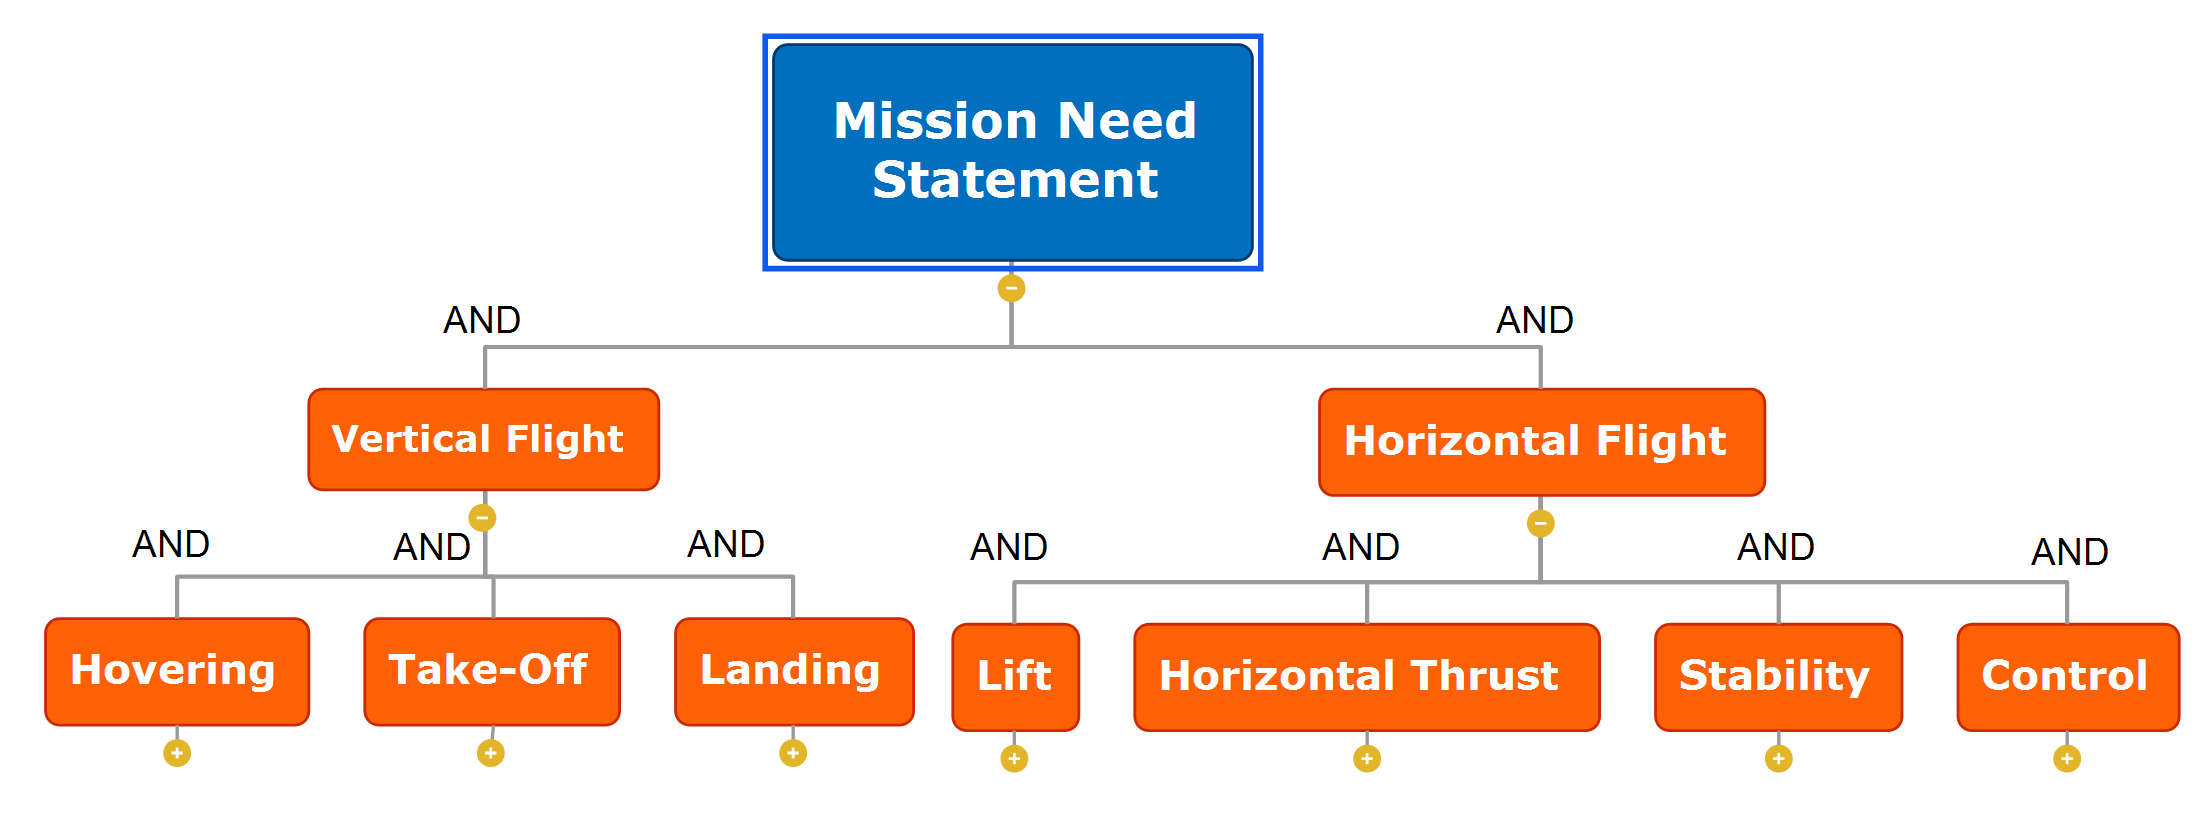
\includegraphics[width=.55\textwidth]{Concepts/Figures/Toplevel}
\caption{Unexpanded design option tree}
\label{fig:DOTmain}
\end{figure}

The first function depicted in the tree is hovering, which is shown in \autoref{fig:DOThover}. This is a major part in various missions, for example monitoring and dropping payload off. There are two branches in the separate hovering tree, propulsion or buoyancy. These two have been chosen by looking at how it is possible to keep an aircraft in the air while stationary. For propulsion there is a whole set of possibilities to get this done, and there are also a lot of possibilities where to get the energy from. This is why this part (under propulsion) is an and-tree. This tree is shown separately in \autoref{fig:DOTprop}. The next part of the branch is buoyancy, which can be achieved with a balloon.

\begin{figure}[H]
\centering
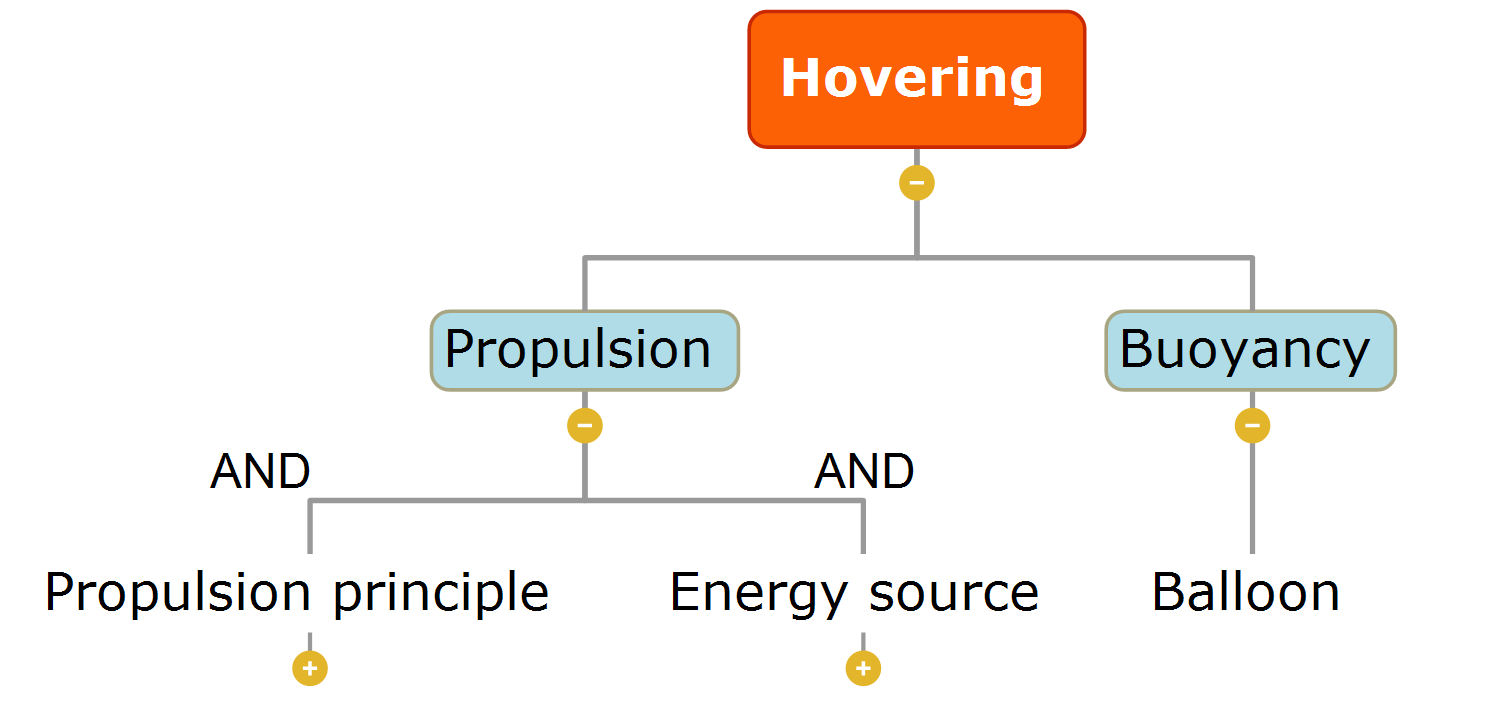
\includegraphics[width=.5\textwidth]{Concepts/Figures/Hovering}
\caption{Hovering branch of the design option tree}
\label{fig:DOThover}
\end{figure}

\autoref{fig:DOTvto} depicts the vertical take-off branch of the design option tree. The vertical take-off functionality is of major importance to the Hybrid UAV design. It allows for operation from almost any location, independent from available ground based infrastructure. This branch is split into three possible means of performing a vertical take-off. These are the light blue coloured blocks on the second level. They are propulsion, buoyancy and kinetic impulse. So, the possibilities are self propelled vertical take-off, lighter than air lift-off or an initial amount of kinetic energy being transferred to the vehicle. The propulsion branch consists of both propulsion principle and energy source. The deeper levels of the propulsion branch of this tree are shown in \autoref{fig:DOTprop} and they will be elaborated on later in this chapter. For buoyancy one can make use of a balloon. For the option of proving an external kinetic impulse to the vehicle there are multiple possibilities. The first method is a sling shot which transfers potential energy from an elastic band to the UAV or a catapult with the similar method. The third method is the trebuchet which transfers gravitational potential energy from a mass to the vehicle.

\begin{figure}[H]
\centering
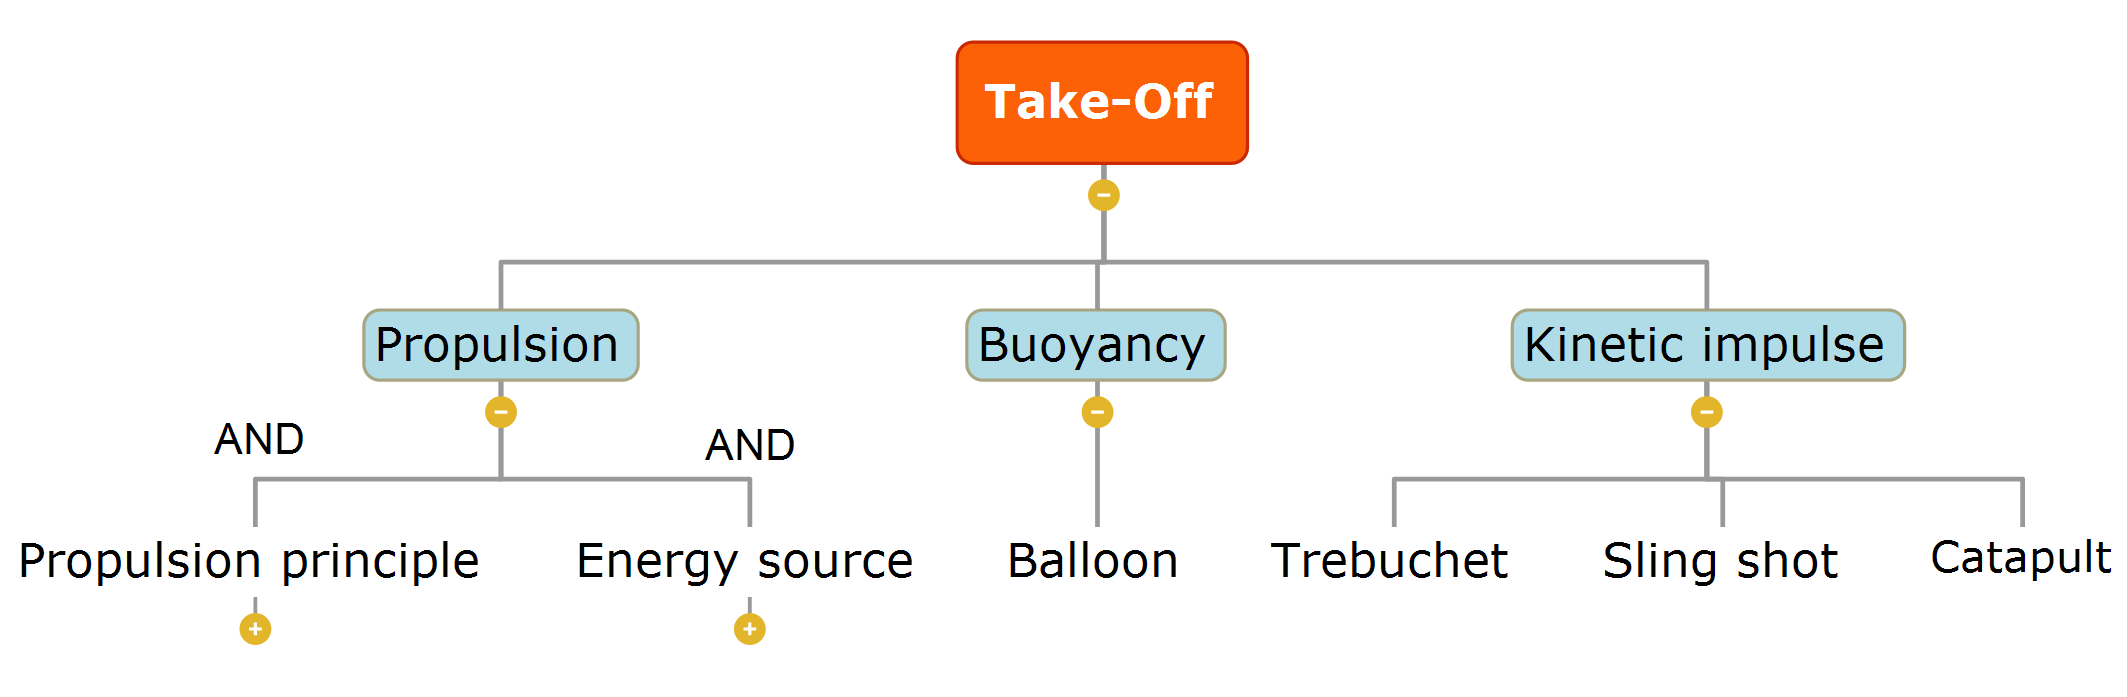
\includegraphics[width=.8\textwidth]{Concepts/Figures/Take-off}
\caption{Vertical take-off branch of the design option tree}
\label{fig:DOTvto}
\end{figure}

The vertical landing capability is a vital element of the Hybrid UAV. It is important for operations on all terrains and reusablity. The vertical landing branch is shown in \autoref{fig:DOTvl}. The propulsive and buoyant options are similar to those in the vertical take-off branch. The option of impact landing is split into three different options. For all of these the vehicle will land vertically with a relatively high velocity and its kinetic energy is absorbed either internally of externally on impact. The impact energy can be absorbed by springs or airbags on the vehicle or by a flexible net on which the UAV will land.

\begin{figure}[H]
\centering
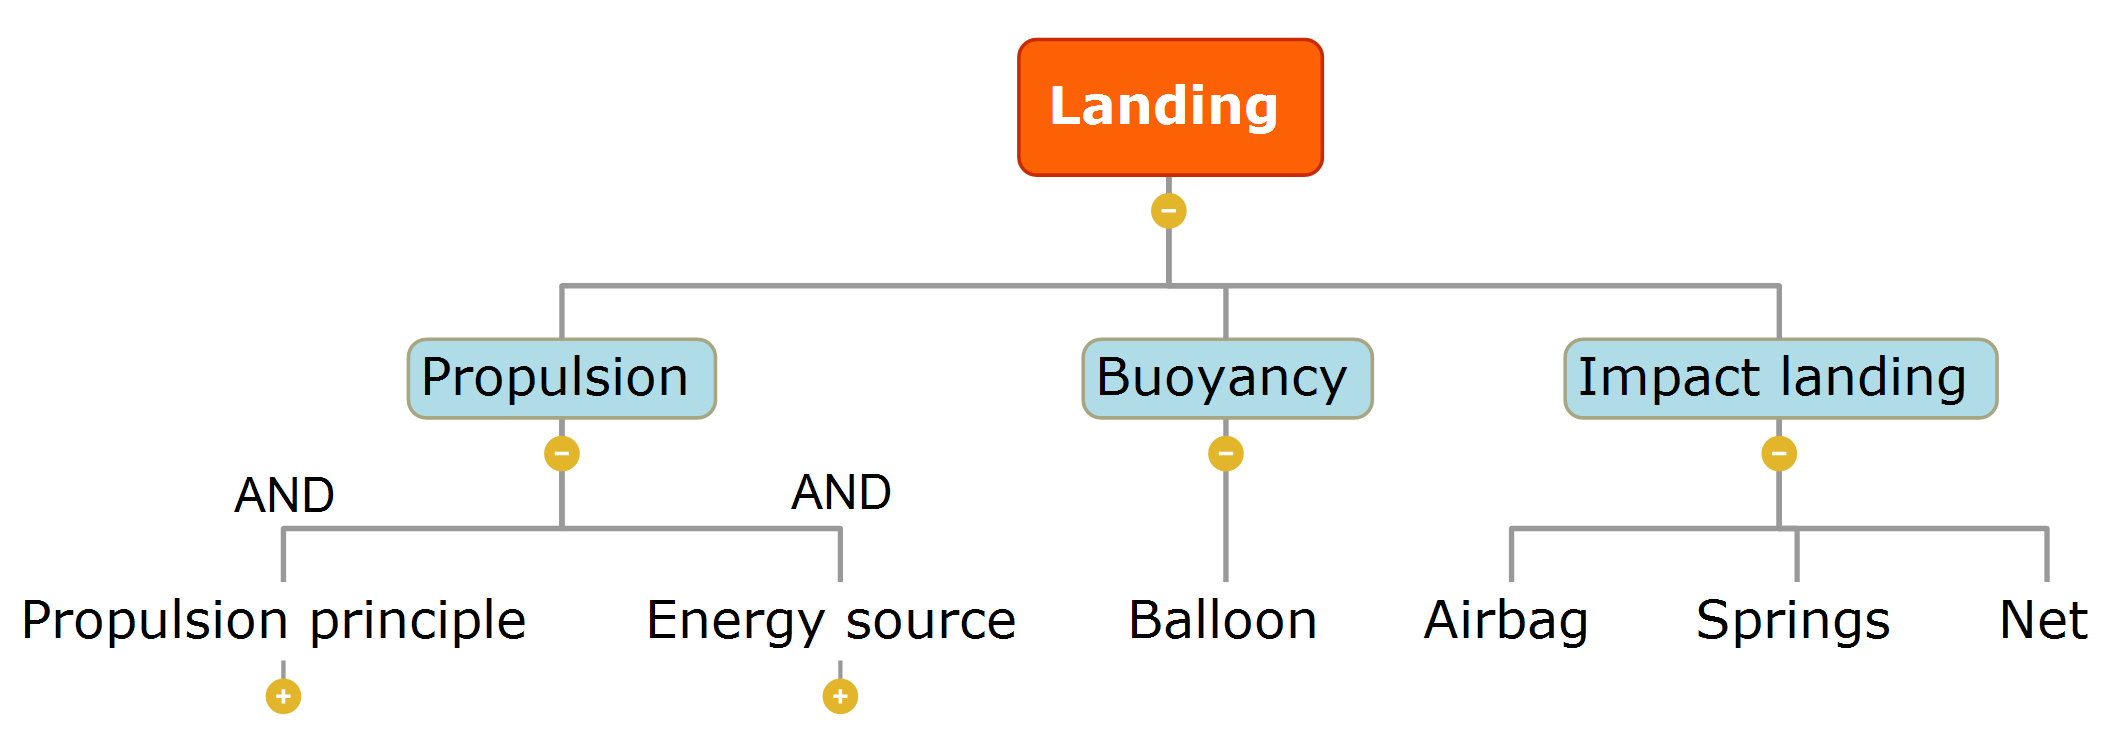
\includegraphics[width=.7\textwidth]{Concepts/Figures/Landing}
\caption{Vertical landing branch of the design option tree}
\label{fig:DOTvl}
\end{figure}

Now that all the functions are done which are connected to VTOL and hovering, it is time to look at how the Hybrid UAV can perform horizontal flight, starting with lift. This branch, shown in \autoref{fig:DOTlift}, is similar to that of the hovering, this is because for hovering you also need to generate some upward force. The main difference here is that you can make use of wings due to the horizontal speed, which is the third branch of this tree. It is possible to have a different amount of wings.

\begin{figure}[H]
\centering
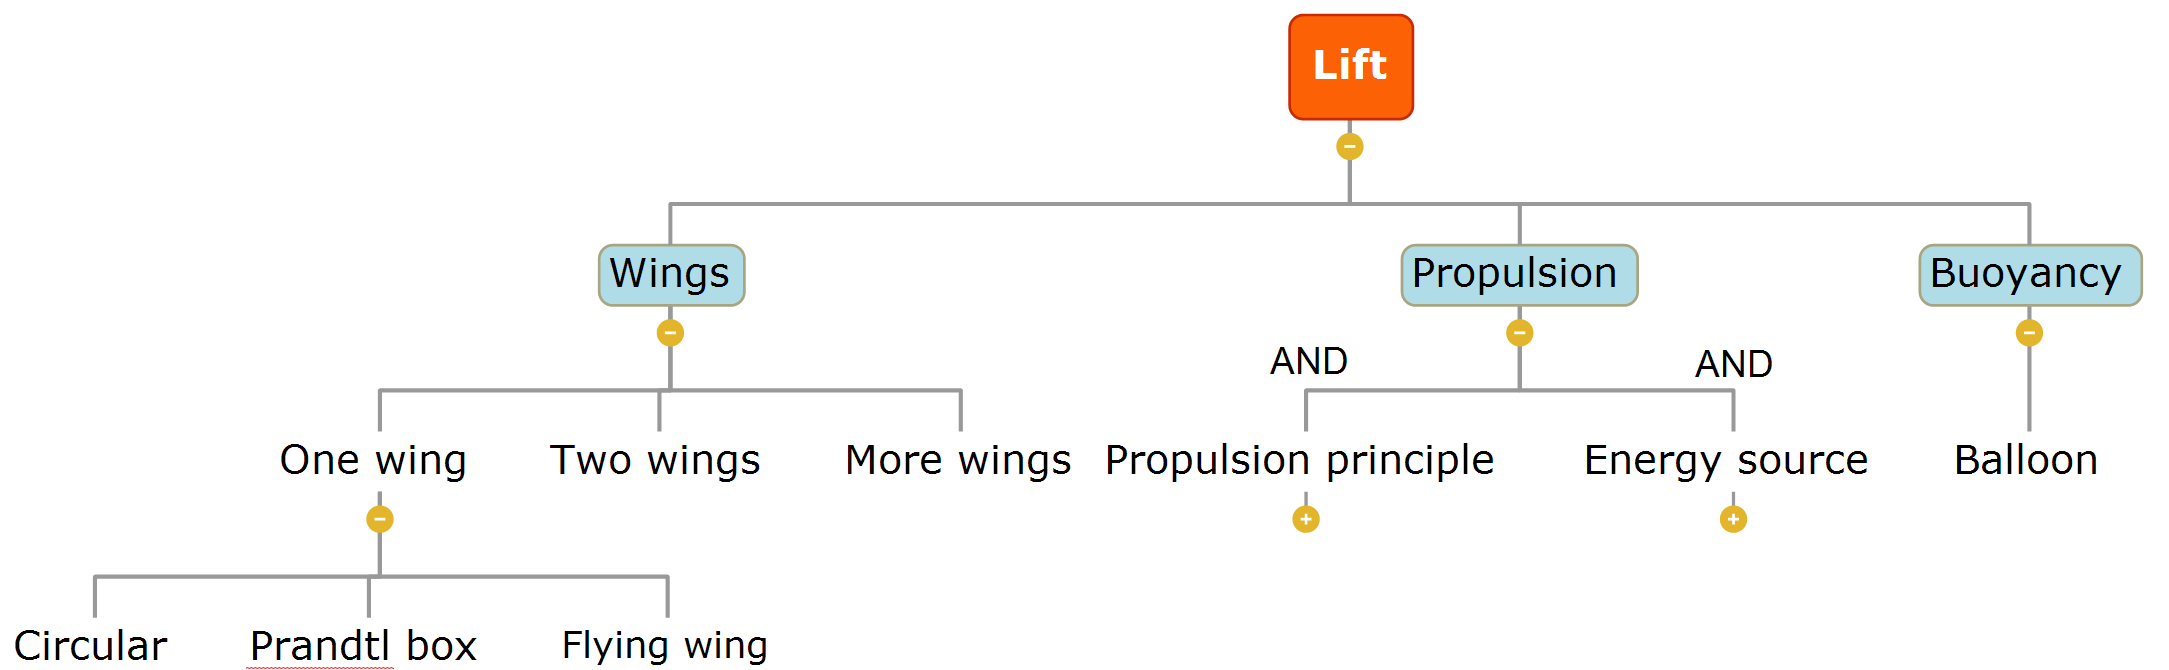
\includegraphics[width=1\textwidth]{Concepts/Figures/Lift}
\caption{Lift branch of the design option tree}
\label{fig:DOTlift}
\end{figure}

\autoref{fig:DOThthrust} shows the choices that there are for the horizontal thrust. When looking at it, it becomes clear that the choices depends on the propulsion, and that there are no other choices. The propulsion AND-tree is shown in \autoref{fig:DOTprop}.

\begin{figure}[H]
\centering
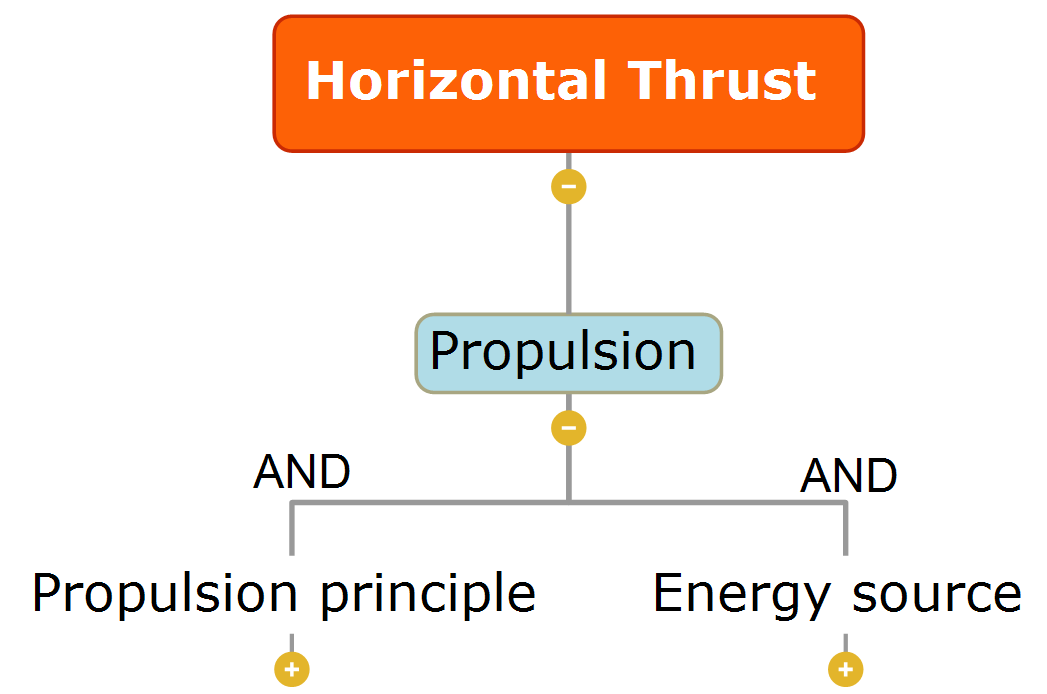
\includegraphics[width=.35\textwidth]{Concepts/Figures/Horizontal_Thrust}
\caption{Horizontal thrust branch of the design option tree}
\label{fig:DOThthrust}
\end{figure}

In \autoref{fig:DOTstability} the stability block of the design option tree is further expanded. It is possible to have active and passive control for this function. The active control can be done with control surfaces or by shifting the mass. For the passive stability the aircraft can make use of an empennage, it can have a dihedral or a sweep for improved stability, or it can use a ballast.

\begin{figure}[H]
\centering
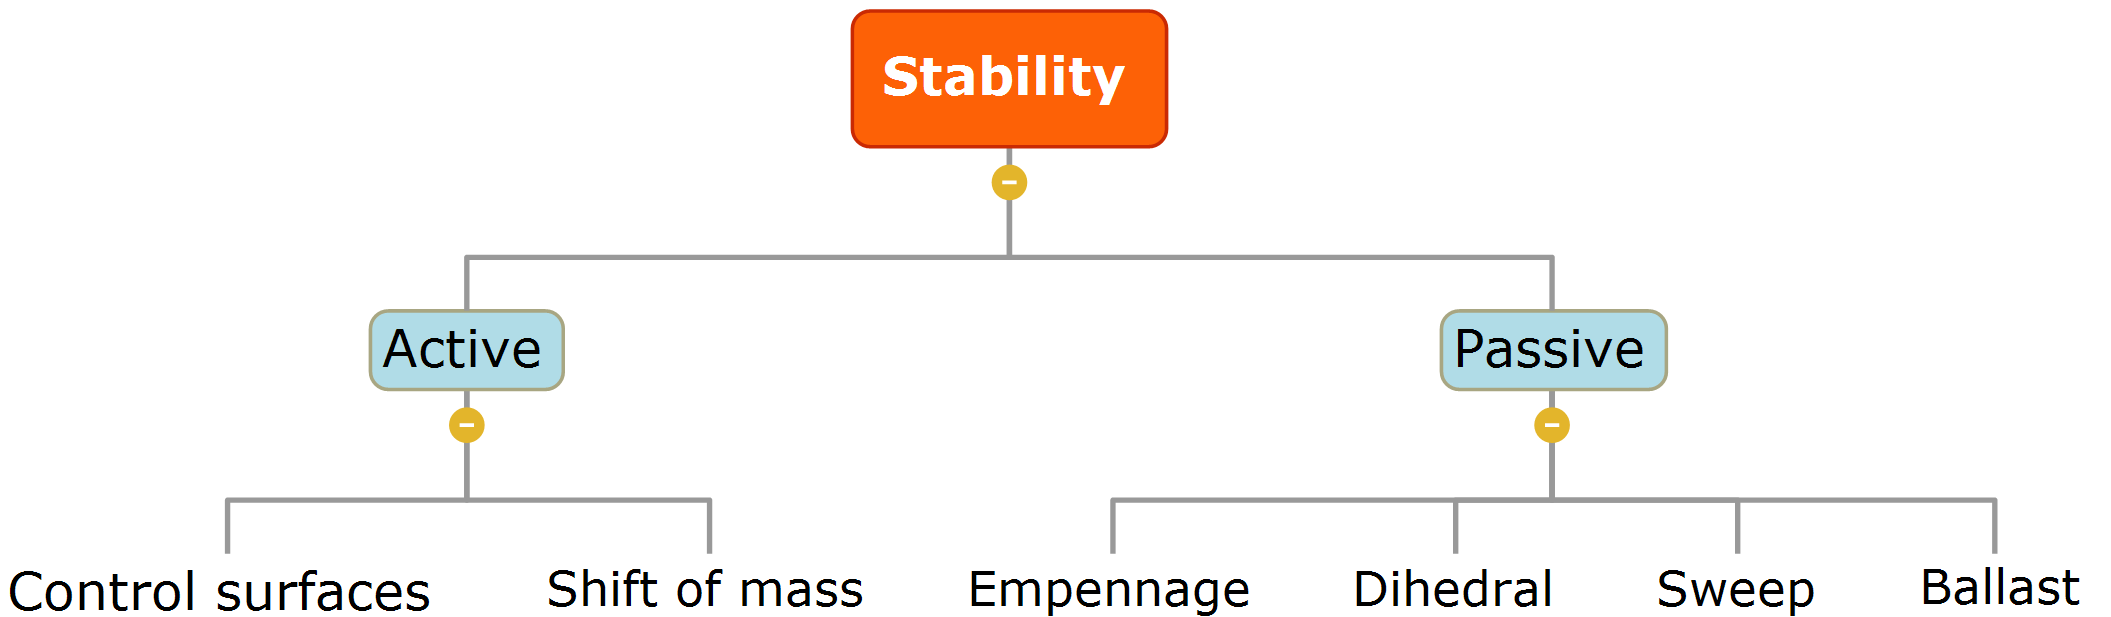
\includegraphics[width=.25\textwidth]{Concepts/Figures/Stability}
\caption{Stability branch of the design option tree}
\label{fig:DOTstability}
\end{figure}

The last function can be seen in \autoref{fig:DOTcontrol}, it depicts how it is possible to control the aircraft. To do this, the aircraft could make use of control surfaces, have morphing wings, shift its mass or make use of plasma air control.

\begin{figure}
    \centering
    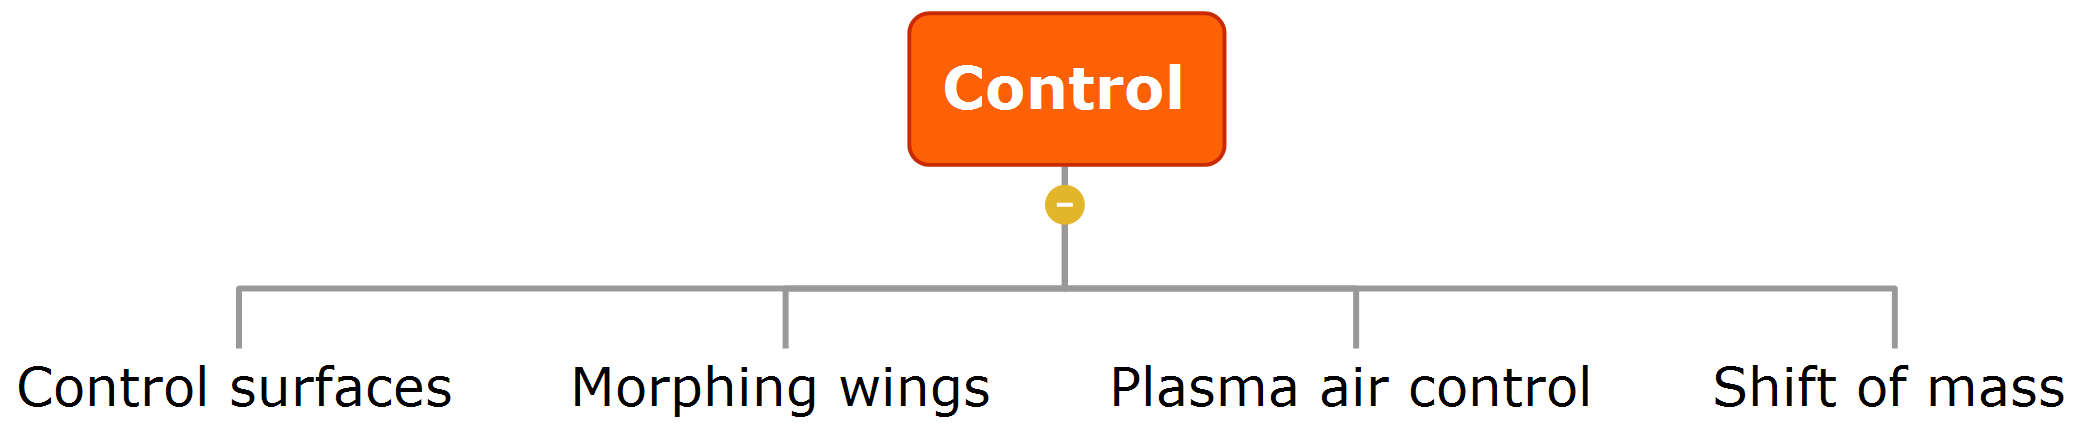
\includegraphics[width=.25\textwidth]{Concepts/Figures/Control}
    \caption{Caption}
    \label{fig:my_label}
\end{figure}

The breakdown of the propulsive options is depicted in \autoref{fig:DOTprop}. The top level propulsion block comprises of both propulsion principle and energy source. The propulsion principle branch on the left side of the tree contains various means of achieving propulsion. On the right side of the tree the energy source branch shows the various methods how to store energy and what kind of energy can be used for propulsion.

\begin{figure}[H]
\centering
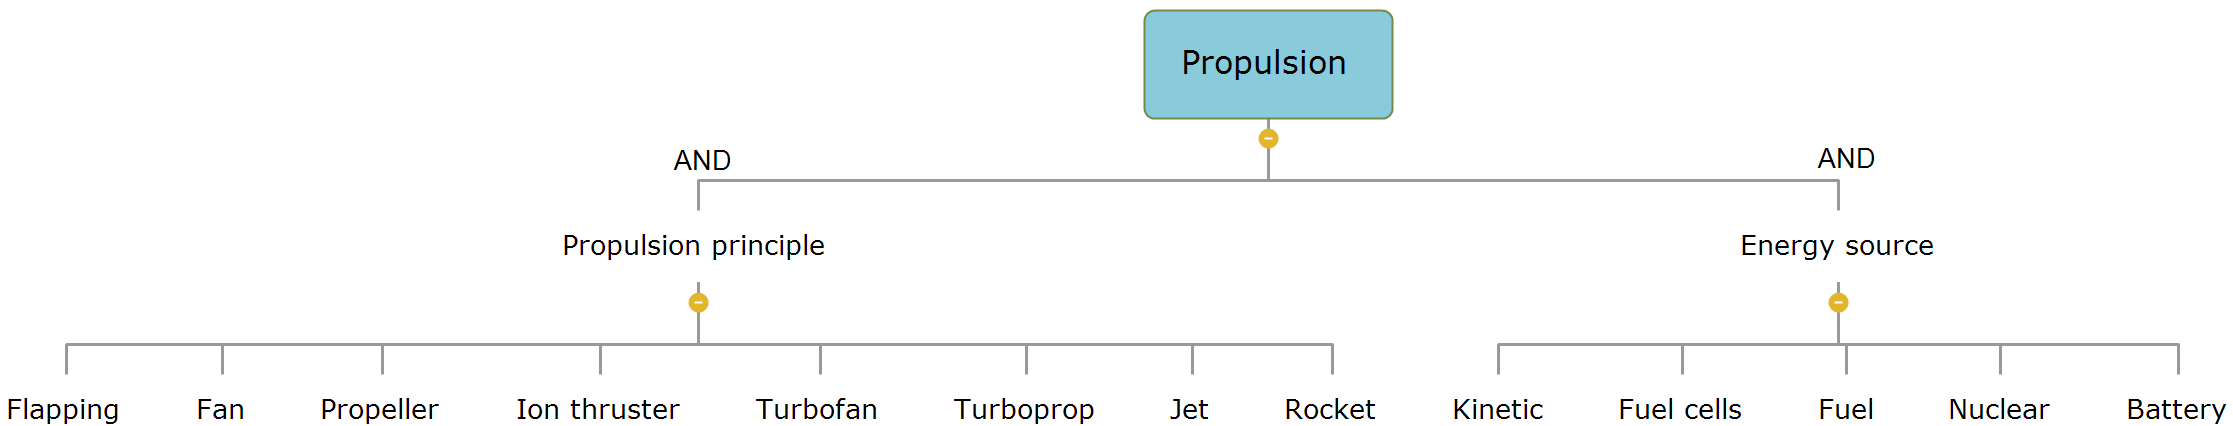
\includegraphics[width=1\textwidth]{Concepts/Figures/Propulsion}
\caption{Propulsion branch of the design option tree}
\label{fig:DOTprop}
\end{figure}

\section{Feasibility Calculations}
\label{sec:feas_calc}
In this section, the airplane-balloon configuration and the Flying Ducted Wing are analysed in a general way to check whether they are feasible concepts or not.

\subsection{Airplane-balloon Configuration}
In order to achieve vertical take-off, landing and hovering for this concept, an inflatable helium balloon is used and needs to generate enough lift. A size of the balloon is estimated based on a simple calculation. A preliminary weight estimation suggests that the UAV weighs 86 kg \cite{baseline}. The density of helium as gas is 0.1664 kg/m$^3$\footnotemark, while that of air is 1.225 kg/m$^3$. Every kilogram of helium can lift 6.3 kg.

%For this concept, the vertical take-off, landing and hovering will be performed using an inflatable helium balloon. In order to do this, the balloon needs to be able to generate enough lift. To check for feasibility, a simple calculation is made. This to estimate the order of the size of the balloon. A preliminary weight estimate of the UAV is 86 kg \cite{baseline}. Since the density of helium, as a gas, is approximately 0.1664 kg/m$^3$\footnotemark, while that of air is approximately 1.225 kg/m$^3$, every kilogram of helium can lift approximately 6.3 kg. 
$$ \frac{1.225}{0.1664} - 1 = 6.3$$

\footnotetext{\url{http://www.engineeringtoolbox.com/gas-density-d_158.html}, Accessed 10-05-2017}


This means 14 kg of Helium is needed to lift the UAV. It requires a balloon of 85 m$^3$, equivalent to 85000 litres. Because of the unrealistic size of the balloon, the balloon concept is deemed infeasible and therefore removed from further development.

\subsection{Flying Ducted Wing}
The flying ducted wing concept has integrated ducts that deflect the exhaust air downward, in order to generate vertical forces. These can be used to perform vertical take-off and landing, as well as hovering. The feasibility of this concept is tested by a very general calculation in which the required downward exhaust velocity is estimated. It is assumed the outlet diameter equals 15 cm, based on the payload. In the case of four ducts, the outlet flow velocity should be in the order of 100 m/s. As the horizontal velocity is zero when taking off, the air should be accelerated from 0 to more than 100 m/s as it will slow down after going through the duct. Therefore, this concept is deemed infeasible.
$$F = \dot{m} v = \rho A v^2 $$
$$v^2 = \frac{F}{4 \cdot \rho A} = \frac{9.81 \cdot 86}{4 \cdot 1.225 \cdot 0.15^2 \cdot \frac{\pi}{4}}$$

\nomenclature[G]{$\rho$}{Density \nomunit{kg/m$^3$}}

\section{Chosen Concepts}
\label{sec:chosconc}

Based on the above calculations, both the airplane-balloon configuration as well as the flying ducted wing will not be analysed any further. It is decided to continue with the remaining three concepts. In order to make sure that enough concepts are compared, two extra concepts are added. These are a tailsitter and a UAV that is a combination of a quadcopter and a conventional aircraft. A summary of each concept is given in this section. Since the manner in which the payload is mounted has not been discussed for the concepts, it will also be elaborated in this section. Different concepts make use of different payload mounting methods, but they all have in common that they enable monitoring equipment to be placed at the bottom of the UAVs and it is possible to release the payload while hovering. 

\begin{comment}
- Door in the fuselage at the end
- Opening on bottom of FL
- click mechanism closed or open
- Removable payload section as part of fuselage
\end{comment}

\subsection{Concept \#1: The Tailsitter}
The Tailsitter can be seen in \autoref{fig:tail_conc}. It does not have movable wings of propellers. Instead, the entire UAV rotates when transitioning from vertical to horizontal flight. Since this is a proven concept\footnotemark, no extra calculations are made before performing the technical analysis. 

In terms of payload mounting, The Tailsitter poses the most difficulty using the payload for monitoring operations. This is because while hovering, the payload area facing downward is 15 x 15 cm instead of 15 x 100 cm as is the case for the other concepts. Therefore, the recording part of the monitoring payload can not be as large in this design as it could in others. The payload will be loaded through the tail. Any payload module should have the same end, that can click into the back. The UAV can then simply release the module and drop it to a designated area.

\footnotetext{\url{http://www.atmosuav.com/}, Accessed 09-05-2017}


\begin{figure}[htb]
\centering
\begin{minipage}{.5\textwidth}
  \centering
  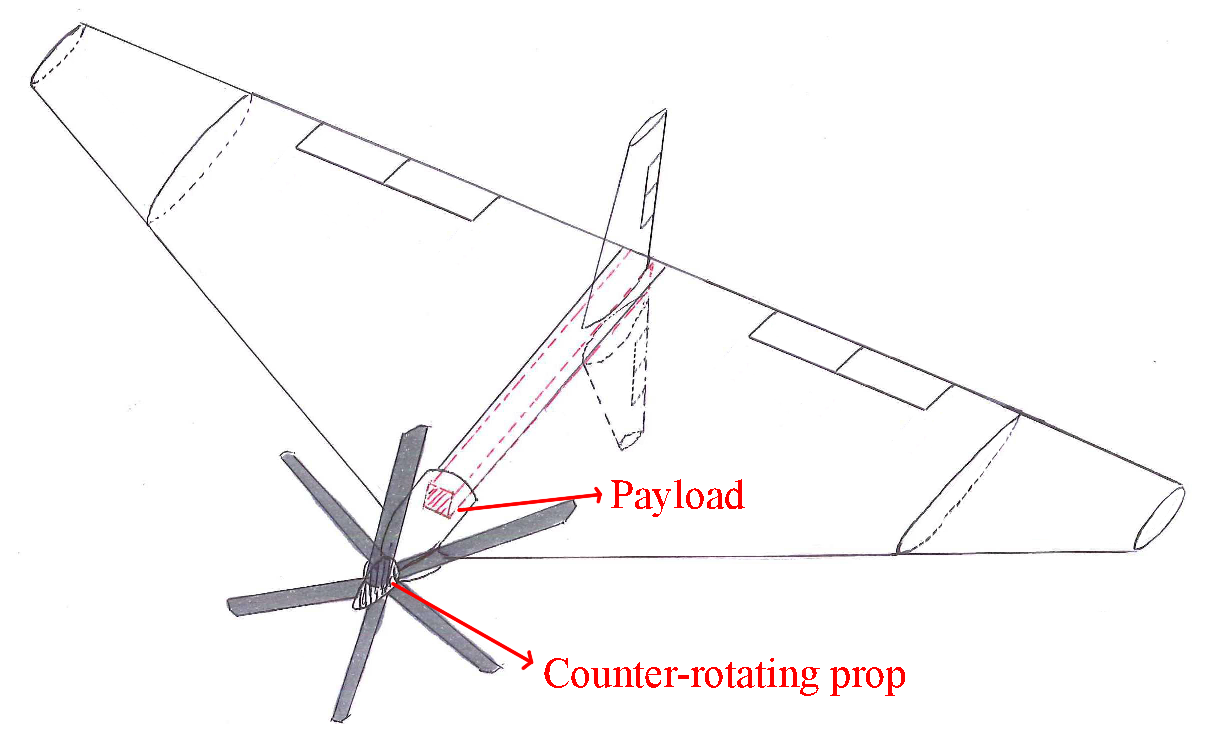
\includegraphics[width=.95\linewidth]{Concepts/Figures/Tailsitter}
  \captionof{figure}{Concept 1: The Tailsitter}
  \label{fig:tail_conc}
\end{minipage}%
\begin{minipage}{.5\textwidth}
  \centering
  \includegraphics[width=.95\linewidth]{Concepts/Figures/Tandem}
  \captionof{figure}{Concept 2: The Tandem}
  \label{fig:tand_conc}
\end{minipage}
\end{figure}


\subsection{Concept \#2: The Tandem}
The tandem concept was already explained in the baseline report \cite{baseline}. It consists of a tandem wing configuration where the wings can be rotated. The layout of the concept can be seen in \autoref{fig:tand_conc}. The feasibility of this concept has been proven\footnotemark.
\footnotetext{\url{http://www.airbusgroup.com/int/en/news-media/media~item=f2c37ffd-dbe4-41c0-b017-ba8ca60bce25~.html}, Accessed 10-05-2017}

The payload can be loaded and unloaded through the back of the fuselage section, where a 'door' is present. In case monitoring equipment is required, the fuselage should contain see-through sections at the bottom. 


\subsection{Concept \#3: The Prandtl Box}
%all that needs to be done is to insert the sketch! name it Prandtl Box
The Prandtl Box analysed in this report has been altered slightly from the concept presented in the baseline report\cite{baseline}. It is done because integrating the propellers in the wing sets a limit on the size of the blades. In the altered concepts, the wing configuration is the same, but the propulsion system is placed in a different location. In the altered setup, this concept has been proven to be feasible\footnotemark. The updated concept can be seen in \autoref{fig:pran_box_conc}
\footnotetext{\url{http://www.avy.eu}, Accessed 10-05-2017}.

The payload will be loaded using a door-like device on the bottom of the UAV. This allows for easy unloading while hovering.

\begin{figure}[htb]
\centering
\begin{minipage}{.5\textwidth}
    \centering
    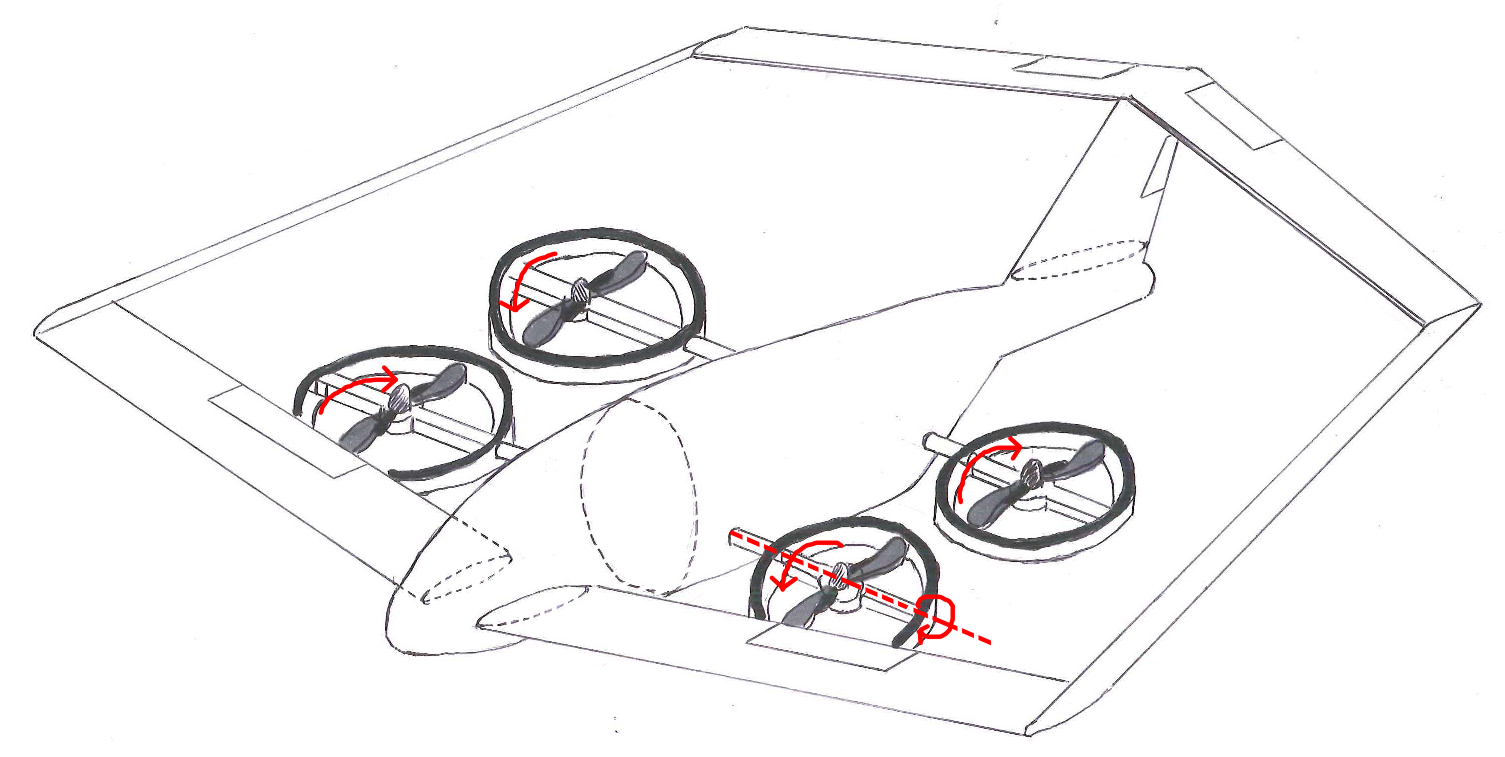
\includegraphics[width = .95\linewidth]{Concepts/Figures/PrandtlBox}
    \captionof{figure}{Concept 3: The Prandtl Box}
    \label{fig:pran_box_conc}
\end{minipage}
\begin{minipage}{.49\textwidth}
    \centering
    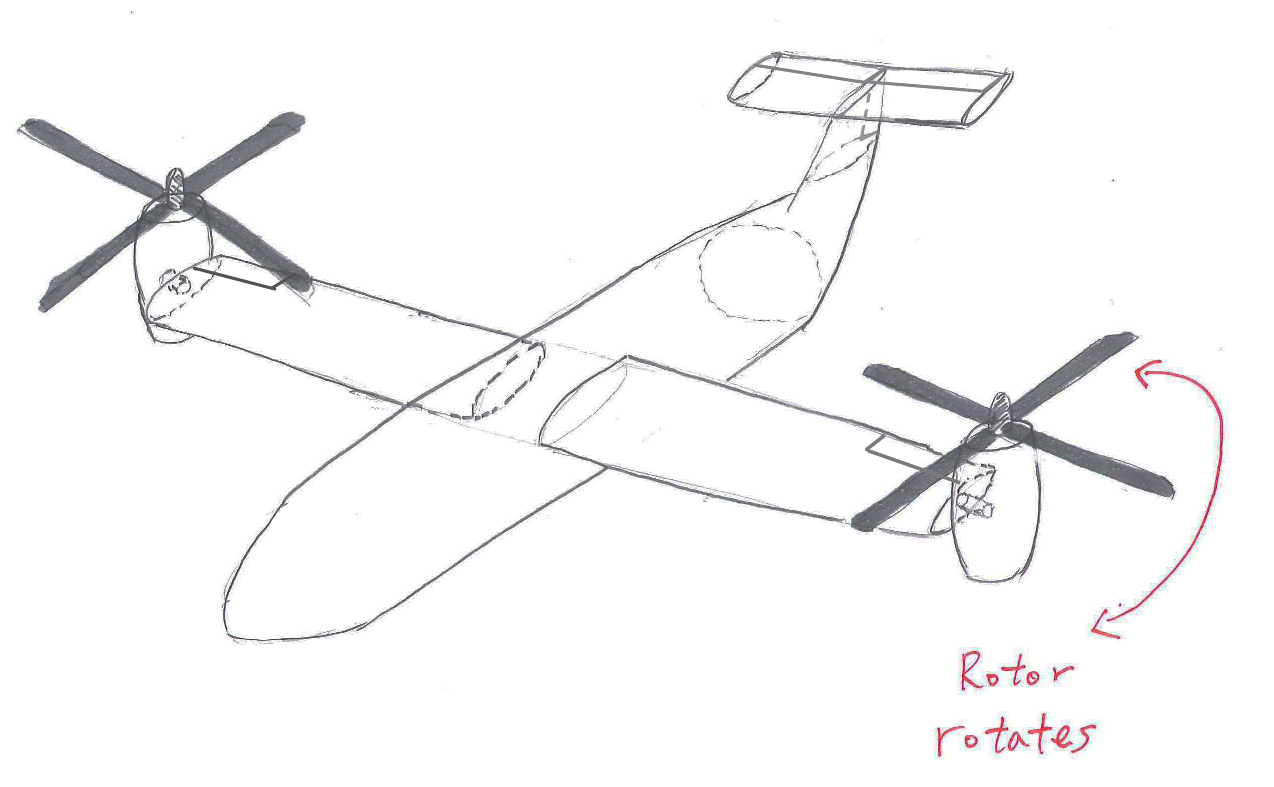
\includegraphics[width=.95\linewidth]{Concepts/Figures/TiltRotor}
    \captionof{figure}{Concept 4: The Tiltrotor}
    \label{fig:tilt_roto_conc}    
\end{minipage}
\end{figure}




\subsection{Concept \#4: The Tiltrotor}
The Tiltrotor is already explained in the baseline report \cite{baseline}. It consists of a fuselage with a wing, where the rotors are attached at the tip of the wing. It is possible to rotate the rotors for horizontal and vertical propulsion. The Tiltrotor can be seen in \autoref{fig:tilt_roto_conc}

The payload will be mounted using a separate payload module that is mounted to the fuselage using a clicking device. The entire payload module can exit the aircraft.




\subsection{Concept \#5: The Winged Quadcopter}
Based on a team discussion, it is decided that a working hybrid UAV design should be included in the analysis. Thus, a winged quadcopter configuration\footnote{\url{https://latitudeengineering.com/products/hq/}, Accessed 10-05-2017} is chosen for analysis. The design can be seen in \autoref{fig:wing_quad_conc}.

% Since two unfeasible concepts were eliminated, time is available to analyse another concept. It was decided that a winged quadcopter configuration will be analysed, because it is one of the most frequently used layouts for hybrid UAVs\footnote{\url{https://latitudeengineering.com/products/hq/}, Accessed 10-05-2017}. The suggested layout can be seen in \autoref{fig:wing_quad_conc}

\begin{figure}[htb]
    \centering
    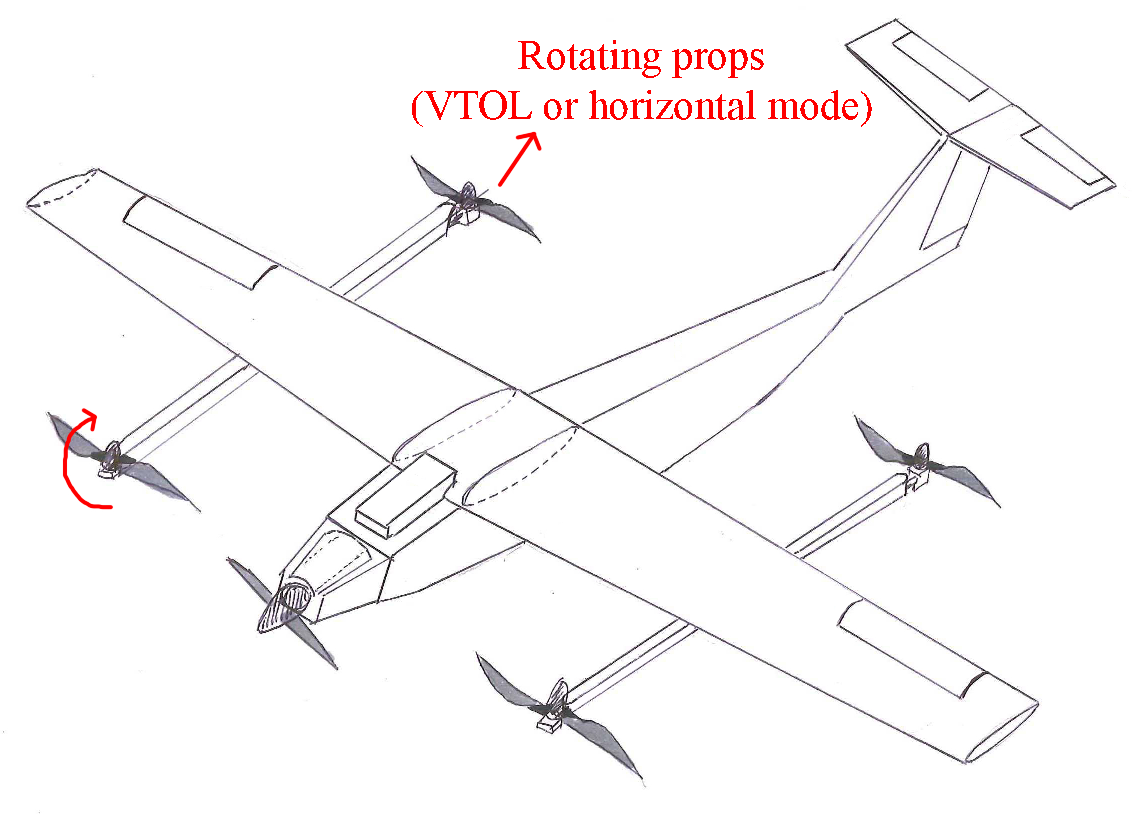
\includegraphics[width=.475\textwidth]{Concepts/Figures/WingedQuadcopter}
    \caption{Concept 5: Winged Quadcopter}
    \label{fig:wing_quad_conc}
\end{figure}

The payload will be mounted similar to the one in The Tiltrotor using a separate payload module that can be replaced and clicked into the fuselage.
    \chapter{Trade-Off}
\label{ch:trad_off}
\setlength{\parindent}{15pt}

With the concepts chosen it is time to perform a trade-off to see which concept has the greatest potential to meet the expectations of the stakeholders. This assessment is critical to the project since it is not possible to enter the preliminary design phase with all of the concepts due to time and resource limitations. Therefore, it is crucial that the analysis is complete and unbiased. To achieve this, trade criteria are selected such that it is possible to judge the degree of compliance of all concepts to requirements most important to the stakeholders. The selection of the criteria and their influences on the final concept selection (weighting) are based on requirements that highly influence the design of the UAV, or that are most important to the key stakeholders. The score of each concept (determined by the criteria and their weights) ultimately indicates the most promising design.  

In \autoref{sec:comp_summ} the complete trade-off table is shown first, summarising the results of the sub-trade-offs described later in the report. \autoref{sec:comp_trad_crit} presents the reasoning for the selection of the trade criteria, and \autoref{sec:comp_crit_weig} shows the method of determining the weights of the trade criteria. Finally, the sensitivity analysis of the trade-off method is performed in \autoref{sec:sens_anal}.

\section{Summary}
\label{sec:comp_summ}

%colour codes
%red #FF0000            |   \cellcolor[HTML]{FF0000}
%orange #FF8000         |   \cellcolor[HTML]{FFC000}
%yellow #FFFF00         |   \cellcolor[HTML]{FFFF00}
%light green #00FF00    |   \cellcolor[HTML]{92D050}
%dark green #088A08     |   \cellcolor[HTML]{00B050}
%light blue #0000FF     |   \cellcolor[HTML]{0000FF}
%dark blue #08088A      |   \cellcolor[HTML]{08088A}

This section will present the results of the final trade-off, which can be seen in \autoref{tab:finaltradeoff}. The outcomes of the trade-off will briefly be discussed to get a grasp as to why the concepts scored as they did. Detailed explanation of the separate criteria scores are the result of extensive research on each criterion, the reasoning behind these scores can be found in \Cref{sec:perf_analy,sec:manostab,sec:grouhand,ch:costanal,ch:deverisk,ch:relianal}. For clarity, the table contains colours to give an overview of the severity of the scores. Five colours have been used in a 30-15-10-15-30 spacing (Red, Orange, Yellow, Light Green, Dark Green). This spacing has been used to show more detail around the average than around the extremes. For when there is a lack of colour, each score has a superscript showing which category it scores: 1 = Red, 2 = Orange, 3 = Yellow, 4 = Light Green, 5 = Dark Green. 

\begin{table}[H]
    \setlength\extrarowheight{5pt}
    \setlength\arrayrulewidth{1pt}
    \centering
    \caption{Final Trade-Off}
    \label{tab:finaltradeoff}
    \begin{tabular}{r|>{\centering}p{2.1cm}|>{\centering}p{1.9cm}|>{\centering}p{1.3cm}|>{\centering}p{1.1cm}|>{\centering}p{0.8cm}|>{\centering}p{0.7cm}|>{\centering}p{0.4cm}|c} 
    \textbf{Concept \rotatebox{90}{\hspace{0.5cm}Criterion}}        & 
    \rotatebox{90}{\textbf{Performance}}                            &
    \rotatebox{90}{\textbf{M\&S}}                                   & 
    \rotatebox{90}{\textbf{Reliability}}                            & 
    \rotatebox{90}{\textbf{Production Cost}}                        & 
    \rotatebox{90}{\textbf{Development Risk}}                       &
    \rotatebox{90}{\textbf{Sustainability}}                         &
    \rotatebox{90}{\textbf{Ground Handling}}                        &
    \rotatebox{90}{\textbf{Outcome}}
    \\\hline
    Tailsitter      &
    \cellcolor[HTML]{FFFF00}50$^{^3}$ &
    \cellcolor[HTML]{FFFF00}46$^{^3}$ &
    \cellcolor[HTML]{FFFF00}50$^{^3}$ &
    \cellcolor[HTML]{FFFF00}50$^{^3}$ &
    \cellcolor[HTML]{00B050}75$^{^5}$ &
    \cellcolor[HTML]{00B050}84$^{^5}$ &
    \cellcolor[HTML]{92D050}59$^{^4}$ &
    \cellcolor[HTML]{FFFF00}\textbf{55$^{^3}$}
    \\[5pt]\cline{2-8}\cdashline{1-1}\cdashline{9-9}
    Tandem          &
    \cellcolor[HTML]{FF0000}17$^{^1}$ &
    \cellcolor[HTML]{FFC000}41$^{^2}$ &
    \cellcolor[HTML]{FFC000}43$^{^2}$ &
    \cellcolor[HTML]{FFC000}35$^{^2}$ &
    \cellcolor[HTML]{FFC000}35$^{^2}$ &
    \cellcolor[HTML]{FF0000}25$^{^1}$ &
    \cellcolor[HTML]{FFC000}38$^{^2}$ &
    \cellcolor[HTML]{FFC000}\textbf{33$^{^2}$}
    \\[5pt]\cline{2-8}\cdashline{1-1}\cdashline{9-9}
    Prandtl Box     &
    \cellcolor[HTML]{92D050}67$^{^4}$ &
    \cellcolor[HTML]{FFC000}41$^{^2}$ &
    \cellcolor[HTML]{92D050}68$^{^4}$ &
    \cellcolor[HTML]{FFFF00}50$^{^3}$ &
    \cellcolor[HTML]{92D050}70$^{^4}$ &
    \cellcolor[HTML]{92D050}58$^{^4}$ &
    \cellcolor[HTML]{FFFFFF}54$^{^3}$ &
    \cellcolor[HTML]{92D050}\textbf{58$^{^4}$}
    \\[5pt]\cline{2-8}\cdashline{1-1}\cdashline{9-9}
    Tiltrotor       &
    \cellcolor[HTML]{FF0000}17$^{^1}$ &
    \cellcolor[HTML]{00B050}73$^{^5}$ &
    \cellcolor[HTML]{92D050}66$^{^4}$ &
    \cellcolor[HTML]{FF0000}25$^{^1}$ &
    \cellcolor[HTML]{FFC000}45$^{^2}$ &
    \cellcolor[HTML]{FF0000}17$^{^1}$ &
    \cellcolor[HTML]{FFFF00}51$^{^3}$ &
    \cellcolor[HTML]{FFC000}\textbf{42$^{^2}$}
    \\[5pt]\cline{2-8}\cdashline{1-1}\cdashline{9-9}
    Winged Quad.    &
    \cellcolor[HTML]{00B050}83$^{^5}$ &
    \cellcolor[HTML]{00B050}85$^{^5}$ &
    \cellcolor[HTML]{00B050}84$^{^5}$ &
    \cellcolor[HTML]{FFFF00}55$^{^3}$ &
    \cellcolor[HTML]{00B050}95$^{^5}$ &
    \cellcolor[HTML]{00B050}84$^{^5}$ &
    \cellcolor[HTML]{00B050}82$^{^5}$ &
    \cellcolor[HTML]{00B050}\textbf{81$^{^5}$} 
    \\[5pt] \hline\hline
    Weight          &
    24              &
    22              &
    16              &
    14              &
    11              &
    8               &
    5               &
    \\[5pt]
    \end{tabular}
\end{table}

The best concept according to the trade-off is The Winged Quadcopter, it scores best in all criteria. For some criteria the difference between the second best is 23, being much better than the other concepts. The final score of The Winged Quadcopter is 81, which is 23 better than the second best concept, The Prandtl Box. 

%%%%%%Extra table if colours need changing, do not delete%%%%%%

%\begin{table}[H]
%    \setlength\extrarowheight{5pt}
%    \centering
%    \caption{Cost sub trade-off}
%    \label{tab:costsubtradja} %please use your own label when you copy it!
%    \begin{tabular}{r|>{\centering}p{2.4cm}:>{\centering}p{2.2cm}:>{\centering}p{1.6cm}:>{\centering}p{1.4cm}:>{\centering}p{1.1cm}:>{\centering}p{0.8cm}:>{\centering}p{0.5cm}|c} 
%    \textbf{Concept \rotatebox{90}{\hspace{0.5cm}Criterion}}    & 
%    \rotatebox{90}{\textbf{Performance}}                      &
%    \rotatebox{90}{\textbf{M\&S}}                           & 
%    \rotatebox{90}{\textbf{Reliability}}                          & 
%    \rotatebox{90}{\textbf{Production Cost}}                      & 
%    \rotatebox{90}{\textbf{Development Risk}}                             &
%    \rotatebox{90}{\textbf{Sustainability}}                            &
%    \rotatebox{90}{\textbf{Ground Handling}}                                   &
%    \rotatebox{90}{\textbf{Outcome}}
%    \\\midrule
%    Tailsitter      & + +   & 46   & 50   & 55   & +     && 59 &  \% 
%   \\[5pt]\hdashline
%    Tandem          & -     & 41     & 43     & 35     & - -  & & 38  &\% 
%    \\[5pt]\hdashline
%    Prandtl Box     & - -   & 41   & 68     & 30     & - -   && UK & \% 
%    \\[5pt]\hdashline
%    Tiltrotor       & 0     & 73   & 66  & 25     & -     && 51 & \% 
%    \\[5pt]\hdashline
%    Winged Quad.    & 0     & 85     & 84     & 60     & + +  & & 82  &\% 
%    \\[5pt] \midrule\midrule
%    Weight          & 24    & 22    & 16    & 14    & 11    &  8  & 5 &\\[5pt]
%    \end{tabular}
%\end{table}

%%%%%%%%%%%%%%%%%%%%%%%%%%%%%%%%%%%%%%%%%%%%%%%%



\section{Trade Criteria}
\label{sec:comp_trad_crit}

The trade criteria have an important impact on the end results of the trade-off. Choosing a criterion which shows no difference in the concepts will jeopardise the trade-off because it will average the results and decrease diversity. This diversity is what should be aimed for to see a distinct difference between the concepts, so that the choice for the final concept will be clear. Each criterion has a separate chapter explaining how it affects each concept, and there is a sub-trade-off showing how each sub-criteria affects the concepts. 

The first criterion, presented in \autoref{sec:perf_analy}, is the performance of the concepts. This criterion has been chosen because there are a lot of requirements on the performance of the aircraft. For this criterion a look will be taken in the mass, the geometric properties, the endurance, the ranged and the power of each concept. The next criterion is the manoeuvrability and stability, shown in \autoref{sec:manostab}. This criterion will perform a sub-trade-off using the manoeuvrability, stability and control of each concept as criteria. Ground handling is the following criterion, taking into account how the concepts can be handled for pre-flight preparations. It can be seen in \autoref{sec:grouhand}. The fourth criterion is the development risk, presented in \autoref{ch:deverisk}. This criterion will not be split into sub-criteria and will have a look to what extent the concepts have been developed already, to assess the risk. The next criterion is the production costs, shown in \autoref{ch:costanal}. This criterion will be split into manufacturing costs, material costs, mechanisms costs, power \& propulsion costs, and finally cost due to weight influence. This criterion has been chosen due to the set limit of 30k for the production, limiting the possibilities for the aircraft. The last criterion is reliability, shown in \autoref{ch:relianal}. This criterion will take a look into the reliability of several systems, including propulsion, control surfaces and wings.

\section{Criteria Weights}
\label{sec:comp_crit_weig}

Weighing the criteria also has an impact on the concept that comes out best. If a not-so-important criteria is weighed more than a criteria which definitely is important, then the results will be misleading. Due to this, the choice was made not to leave the weighing decision solely to one person since it is possible to get biased weights. To find the weights, each member of the team was tasked with filling out a form comparing each criterion to all other ones. Once this was done, the averages of the results were taken. These averages were normalised to ten to get a feel as to how much they score on a scale from one to ten. These normalised scores were then converted into percentages to use for the trade-off. The results can be seen in \autoref{tab:weightoffinaltradeoff}.

\begin{table}[H]
    \centering
    \caption{Criteria Weights for The Final Trade-Off}
    \begin{tabular}{ccc}
    \toprule
    \multirow{2}{*}{\textbf{Criterion}}    &  \textbf{Weight} & \multirow{2}{*}{\textbf{Weight (\%)}}\\
         & \textbf{(Normalised to 10)} & \\ \midrule
    Performance & 9 & 24 \\ \hdashline
    Manoeuvrability & \multirow{2}{*}{8} & \multirow{2}{*}{22} \\
    \& Stability & & \\ \hdashline
    Reliability & 6 & 16 \\ \hdashline
    Production Cost & 5 & 14 \\ \hdashline
    Development Risk & 4 & 11 \\ \hdashline
    Sustainability & 3 & 8 \\ \hdashline
    Ground Handling & 2 & 5 \\ \bottomrule
    \end{tabular}
    \label{tab:weightoffinaltradeoff}
\end{table}

\section{Sensitivity Analysis}
\label{sec:sens_anal}

The goal of the sensitivity analysis is to determine to what extent the final concept selection depends on a change in the weighting of the trade criteria. It alerts whether the chosen concept greatly outperforms all other concepts in one area whilst being poor in the remaining areas. Therefore it is desirable that during the sensitivity analysis the ranking of the concepts do not change. More so, the concept performing best initially, should remain ranked highest at the end of the analysis.

The sensitivity analysis is carried out by successively increasing the weighting of one of the trade criteria, and recalculating the relative score between the concepts. In order to ensure that the analysis is somewhat reliable, the change in weighting should not be too small. An increase of 20\% in the weighting of one criteria yields such results.

\autoref{fig:sensitivityanal} presents a comparison between the scores of the concept corresponding to the changed trade criteria weightings, starting with the original setup. The horizontal axis indicates the type of modified weighting used to achieve the corresponding scores of the concepts. These are the original (normal) weighting and weightings with one criteria increased by 10\%. The score of each concept is shown on the vertical axis.

\begin{figure}[H]
    \centering
    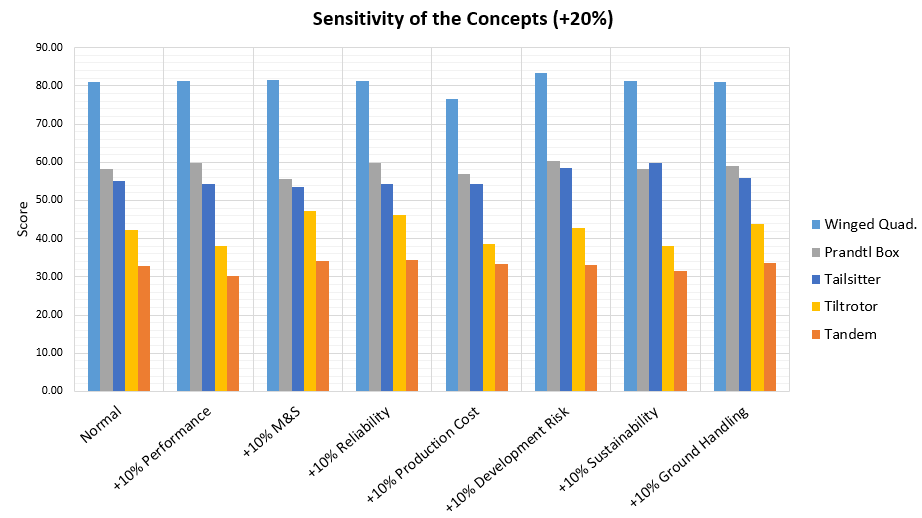
\includegraphics[width=\textwidth]{TradeOff/Figures/sensitivity}
    \caption{Sensitivity Analysis of The Final Trade-Off}
    \label{fig:sensitivityanal}
\end{figure}

The figure shows that even thought the weights of the criteria are changed, The Wing Quadcopter scores highest every time. The gap between the first best and second best does not decrease drastically during the sensitivity analysis, showing that the weighting will not influence the end results. The overall rankings of the concepts also remain unchanged everywhere except when sustainability is weighted 20\% more, this is because The Tailsitter scores 26 higher than The Prandtl Box for that criterion.

Since the Winged Quadcopter greatly outperforms all other concepts throughout the entire sensitivity analysis, it is safe to say that this concept has the greatest potential to satisfy all requirements. Therefore it is sensible to further develop this concept into the preliminary design phase.

 
    %READ THROUGH AND ACCEPTED BY: CHRIS, 23-05-2017 (NO COMPILE)
\chapter{Performance Analysis}
\label{ch:perf_analy}

In this chapter, the performance of each concept is analysed and a trade-off is performed. First, in \autoref{sec:trade_perf}, a summary trade-off table of the whole chapter is illustrated. Then a preliminary mass estimation of each concept is performed in \autoref{sec:mass_esti}, followed by a determination of the geometric properties in \autoref{sec:geom_prop}. Then, the endurance and range properties are analysed in \autoref{sec:endu_ana} and \autoref{sec:range_ana} and finally in \autoref{sec:power_ana} the required power for each concept is calculated. For the different concepts, the used mass estimation methods are not always the same. This has to do with the different available data. 

\section{Performance Trade-Off}
\label{sec:trade_perf}

This section illustrates the final trade-off of the performance analysis. First, a brief summary is shown in \autoref{tab:perform_trade} and then the grading system used for the trade-off is explained.
\subsection{Summary}
\label{sec:perf_sum}

In this section, the final performance trade-off is illustrated in \autoref{tab:perform_trade}. It can be seen, that The Winged Quadcopter and The Prandtl Box score best in terms of performance. This mainly comes from their low mass estimations and higher aspect ratio analysis. Then The Tandem and The Tiltrotor score worst on performance properties. Both of them are complex design which require a high mass in order to attain the required performance set by the stakeholders. 

\begin{table}[H]
    \centering
    \caption{Performance Sub Trade-Off}
    \label{tab:perform_trade} 
    \begin{tabular}{r|>{\centering}p{2.5cm}:>{\centering}p{2.5cm}:>{\centering}p{2.5cm}|c} 
    \textbf{Concept \rotatebox{90}{\hspace{0.5cm}Criterion}}    & 
    \rotatebox{90}{\textbf{Endurance}}                      &
    \rotatebox{90}{\textbf{Range}}                           & 
    \rotatebox{90}{\textbf{Required Power}}                          & 
    \rotatebox{90}{\textbf{Cumulative}}                       
    \\ \midrule
    Tailsitter      & - & 0 & + & 50\% 
    \\\hdashline
    Tandem          & - & - & \texttt{-{}-} & 17\% 
    \\\hdashline
    Prandtl Box     & ++ & + & - & 66.5\% 
    \\\hdashline
    Tiltrotor       & \texttt{-{}-} &  \texttt{-{}-} &  0 & 17\% 
    \\\hdashline
    Winged Quad.    & + & + & ++ & 83\% 
    \\ \midrule\midrule
    Weight          & 0.33  & 0.33  & 0.33  &  
    \end{tabular}
\end{table}

\subsection{Grading System}
\label{sec:grading_sys_perf}

The whole performance chapter uses numerical values in order to obtain trade-off results. As it is not possible yet to accurately generate results due to a lack of battery information and other relevant data, a valid grading system has to be obtained. For this, first the average of all of the values is calculated. Then, the percentage of each value towards the average is used as grading system. The grading system in \autoref{tab:grad_perf} is used. 

\begin{table}[htb]
\centering
\caption{Performance Grading System}
\label{tab:grad_perf}
    \begin{tabular}{ll}
    \toprule
    \textbf{Rating} & \textbf{Percentage of average} \\
    \midrule
    ++ &  more than 130\% of average\\\hdashline
    +  & 110\% up to and including 130\% of average\\\hdashline
    0  & 90\% up to and including 110 \% of average\\\hdashline
    -  & 70\% up to and including 90\% of average\\\hdashline
    \texttt{-{}-}& less than 70\% of average\\
    \bottomrule
    \end{tabular}
\end{table}

\label{sec:perf_appr}

%This chapter did not ahear to the standard structure, is it possible to change it to fit it that way?
% X Ground Handling
% X.1 Trade-Off
% X.1.1 Summary
% X.1.2 Grading System
% X.2 Criteria
% X.2.1 Criteria #1 < explain a bit how it influences
% etc
% X.2.X Criteria Weights
% X.3 Concept Analysis
% X.3.1 Concept 1 < here you explain how much + or - each concept gets for each criteria
% etc

\section{Mass Estimation}
\label{sec:mass_esti}

For the mass estimation, statistical analysis is performed; by means of collecting reference aircraft, the take-off mass estimation for the UAV concepts are obtained. 

Unfortunately, for some concepts no data could be found with comparable performance. In these cases, it has been chosen to use UAVs from a different mass category. By means of finding the $\frac{M_{payload}}{M_{TO}}$ ratio and by taking into account the 10kg payload capacity requirement, a UAV take-off mass estimation can be obtained.

In other words, the payload capacity is scaled according to the payload capacity of 10kg as set in the requirements. In this way an estimated take-off mass is found for the specific configurations that should have the right payload capacity.

\subsection{The Tailsitter}
The Tailsitter concept is based on a flying wing using a rotor on its nose as propulsion system. \autoref{tab:flyingwing} shows the payload and take-off mass of similar UAVs: the Atmos\footnote{\url{http://www.atmosuav.com/}, Accessed 12-05-2017}, the Firefly 6 \footnote{\url{https://www.birdseyeview.aero/}, Accessed 15-05-2017}, the Fury 1500 \footnote{\url{http://www.airforce-technology.com/projects/fury-1500-uav/}, Accessed 12-05-2017} and the Cantas E \footnote{\url{http://newspacetechnologies.cz/cantas-uas-project/}, Accessed 22-05-2017}. It also shows their respective ratio. The average of the ratios is used to calculate a the payload over take-off ratio for The Tailsitter. With this ratio it is possible to calculate the mass.

\begin{table}[htb]
    \centering
    \caption{Flying Wing Reference Aircraft}
    \label{tab:flyingwing}
    \begin{tabularx}{\textwidth}{lccc}
        \toprule
        \textbf{Reference drone}    & \textbf{Payload Mass [kg]}     & \textbf{MTOW [kg]}      & \textbf{Payload/Take-Off ratio}          \\\midrule
        Atmos                       & 0.8                            & 4.5                     & 5.63  \\\hdashline
        Firefly 6                   & 0.7                            & 4.1                     & 5.86 \\\hdashline
        Cantas E                    & 10                             & 65                      & 6.5     \\\hdashline             
        Fury 1500                   & 34                             & 136                     & 4 \\\midrule
        Average                     &                                &                         & 5.49 \\\bottomrule
    \end{tabularx}
\end{table}

The UAV should be able to carry a payload of at least 10 kg, this gives a mass of approximately 55 kg for the Tailsitter concept. 

\subsection{The Tandem}
%written by Bryan and Piotr

 In order to estimate the mass of The Tandem, two reference UAVs are chosen. The first one is the DHL Parcelcopter that has one rotating wing\footnote{\url{http://www.dhl.com/en/press/releases/releases_2016/all/parcel_ecommerce/successful_trial_integration_dhl_parcelcopter_logistics_chain.html}, Accessed 15-05-2017}. 
 
\begin{comment}
\begin{figure}[H]
    \centering
    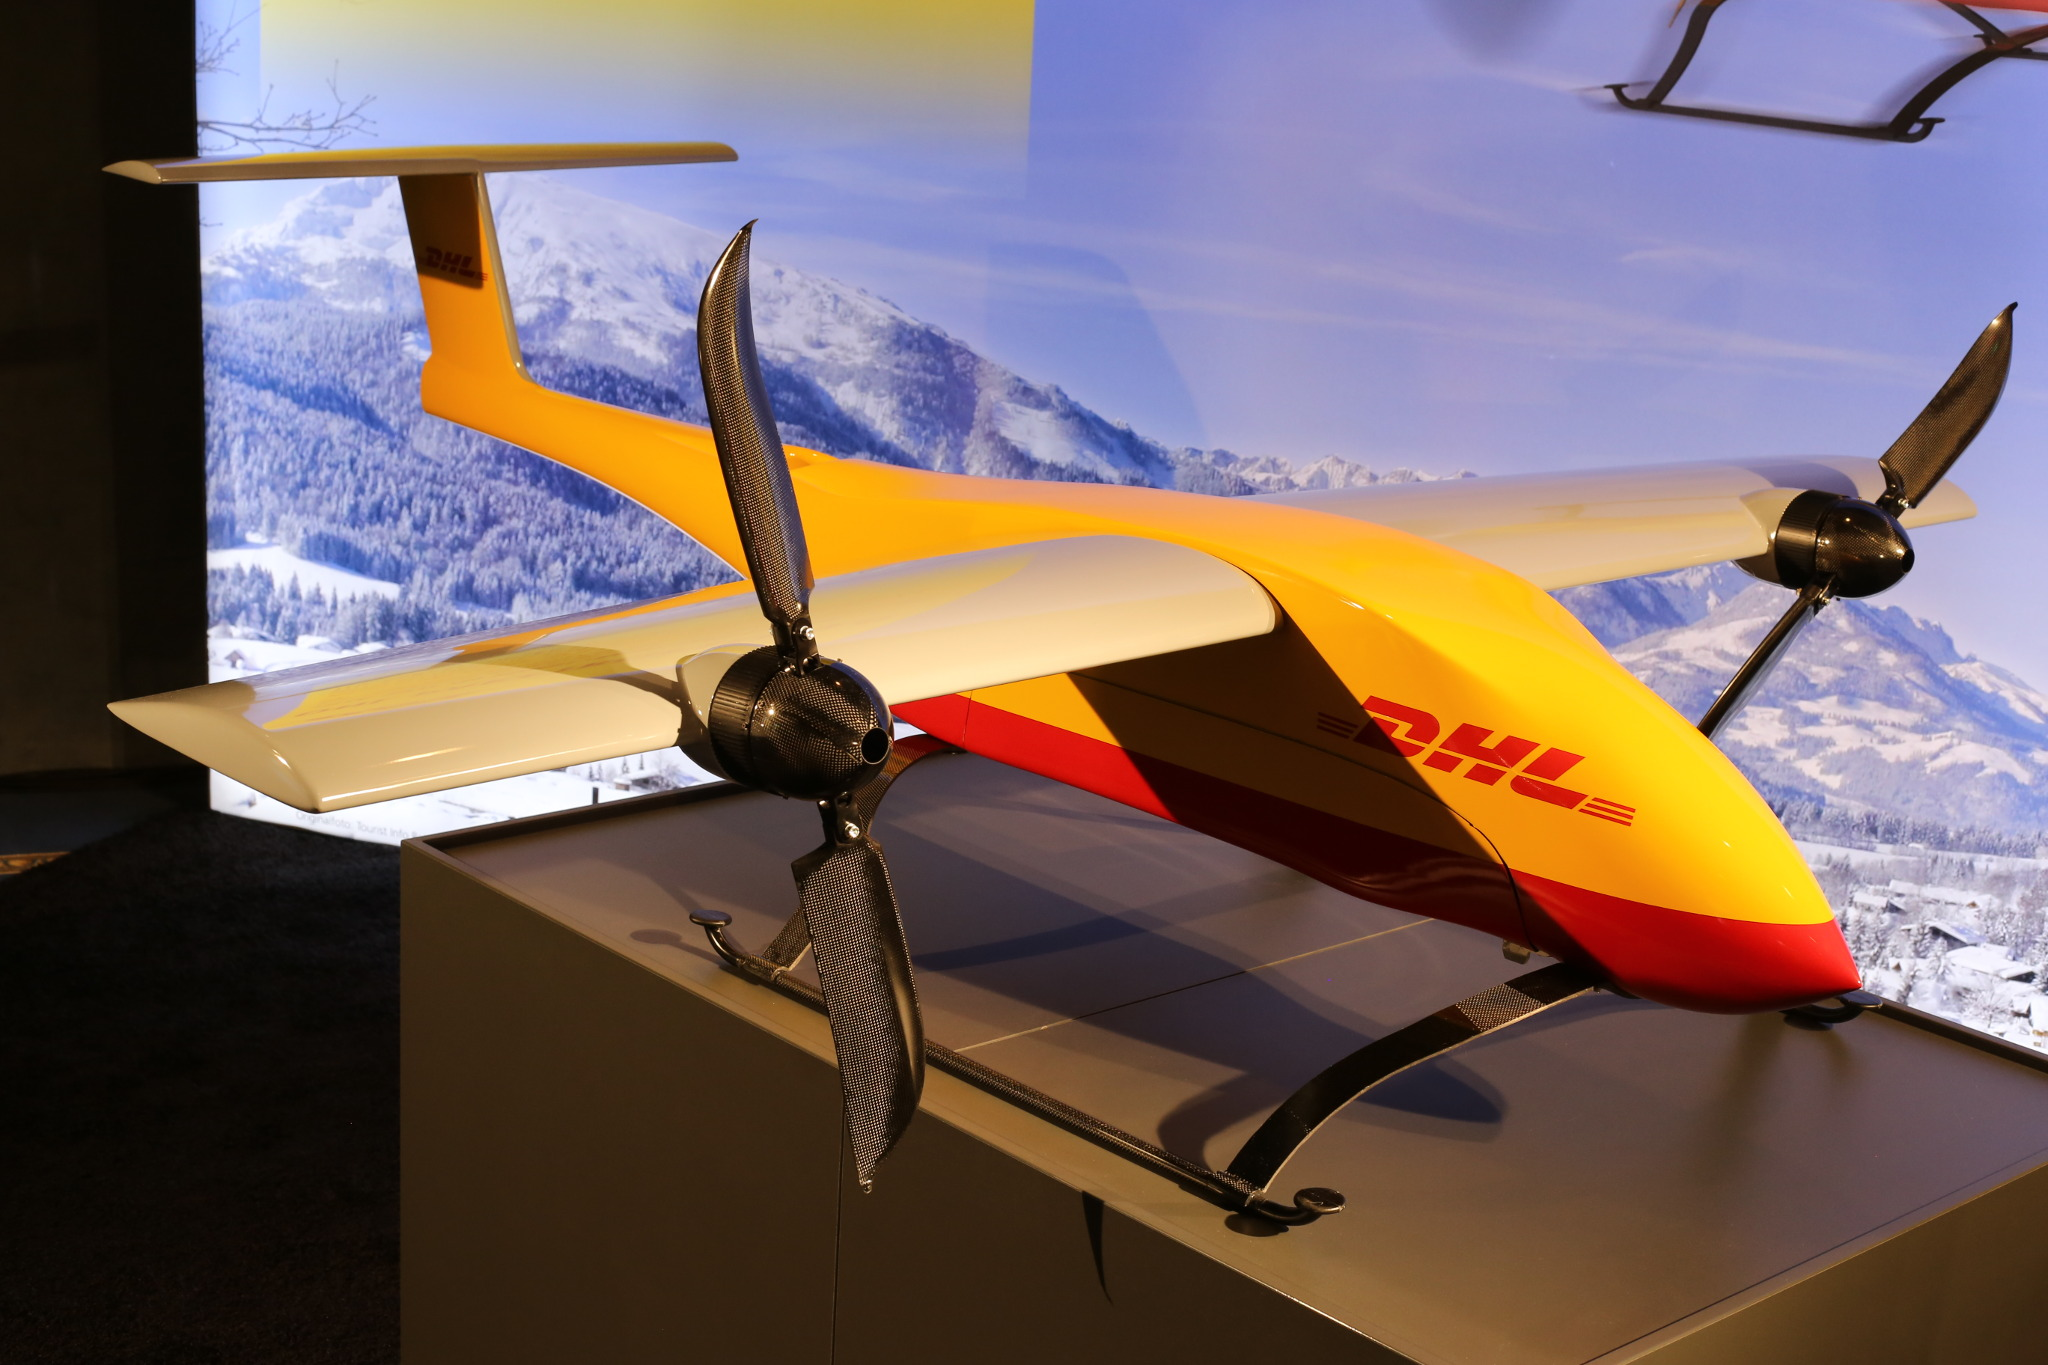
\includegraphics[width=0.6\textwidth]{PerformanceAnalysis/Figures/DHLparcelcopter3.jpeg}
    \caption{DHL Parcelcopter 3.0}
    \label{fig:parcelcopter}
\end{figure}
\end{comment}

The Maximum Take-Off Weight (MTOW) for this UAV is 14 kg, and the corresponding maximum payload mass is 2 kg. Since The Tandem has two rotating wings, additional mass has to be added to Parcelcopter in order to compensate for having only one wing. The structural mass of the wing is approximated to be 10\% of MTOW \cite{uav_weight}, thus having two rotating wings will result in a MTOW increase of 1.4 kg. With MTOW of 15.4 kg and payload of 2 kg, a scaling factor of 5 is applied such that the UAV meets the required payload mass of 10 kg. 

The resulting MTOW of The Tandem is 77 kg, yet it must be noted that The Tandem has no empennage, and intrinsically has a smaller wingspan than the reference aircraft, since the wing surface area can be divided amongst two wings. Both of these factors each reduce the MTOW by 5\% each\cite{uav_weight}. Therefore, the MTOW of The Tandem becomes 70 kg based on an analysis using Parcelcopter. 

The other reference UAV is developed by Chiba University\footnote{\url{http://www.barnardmicrosystems.com/UAV/milestones/tilt_wing.html}, Accessed 22-05-2017}. it has payload mass of 5 kg and MTOW of 23 kg. In order to meet the required payload mass of 10 kg, a scaling factor of 2 is applied. The UAV will have MTOW of 46 kg and payload mass of 10 kg. Due to lack of reference UAVs, data for two reference UAVs is combined in order to carry out a robust analysis. Thus, an average of MTOW is taken. The MTOW of The Tandem is determined to be 58 kg.

\begin{comment}
\begin{figure}[H]
    \centering
    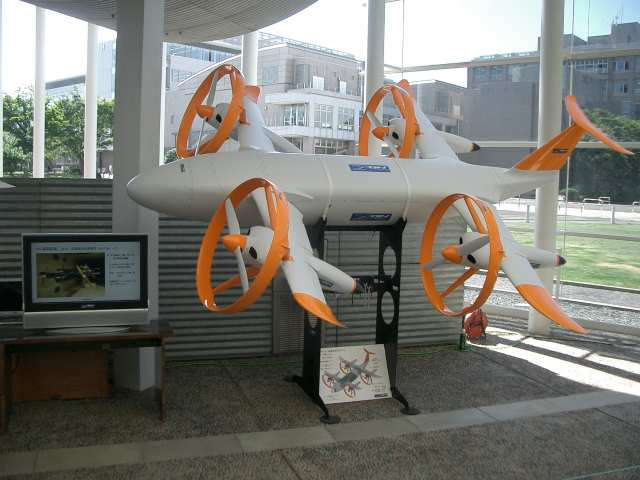
\includegraphics[width=0.6\textwidth]{PerformanceAnalysis/Figures/japtandem.jpg}
    \caption{Chiva University Tandem UAV}
    \label{fig:japtandem}
\end{figure}
\end{comment}
\subsection{The Prandtl Box}

The mass estimation for The Prandtl Box design is based on a comparable design proposed by AVY\footnote{\url{http://www.avy.eu/}, Accessed 12-05-2017}. This design has, with regard to the specifications and performance, much resemblance with the requirements set for this design. The mass of the AVY hybrid UAV can thus be considered as a reliable estimate for this design concept.

AVY claims that the Manufacturer's Empty Weight (MEW) is 13 kg. Based on a definition of MEW, it does not include mass of a battery and payload. By rearranging \autoref{eq:range} and \autoref{eq:endurance}, which can be found in \cref{sec:range_ana,sec:endu_ana}, a preliminary mass of the battery is determined to be 15 kg in order to obtain a range of 200 km and minimum endurance of 1 hour for a conventional-type UAV. With the required payload of 10 kg, the MTOW of The Prandtl Box becomes 38 kg. 

\subsection{The Tiltrotor Concept}
For the mass evaluation of this concept, the mass sensitive components have to be identified. The main component to be considered is the tilting rotor at the wingtips. This component will contribute significantly to the mass of the design. The main reason for this is the fact that the rotatable engines on the wing tips will need strong structural support to counter the strong forces and bending moments it introduces.

%The main reason for this is the fact that these rotating mechanisms have a high level of complexity, this results in an increase of mass. Besides this, there are structural reasons as well; due to the mounting of these complex mechanism at the wing tips, extra structural support is required. Furthermore, the introduction of loads at the wingtips by the engines require more structural support as well. All this extra required structural support will add to the total structural mass of the design.

For the mass estimation the data of three UAVs is consulted. In \autoref{tab:Tilt} the values are documented. By comparing the payload mass over take-off mass ratios of the reference vehicles. The used reference UAVs in this analysis are the Kari TR-60\footnote{\url{http://www.janes.com/article/63543/dx-korea-2016-kari-unveils-tr60-tiltrotor-uav}, Accessed 12-05-2017}, the Bell Eagle Eye\footnote{\url{https://fas.org/irp/program/collect/eagle-eye.htm}, Accessed 12-05-2017} and the Vertex VTOL UAS\footnote{\url{http://www.comquestventures.com/vertex-vtol-uas/\#imageclose-866},  Accessed 12-05-2017}. The Kari TR-60 together with the Vertex VTOL UAS is, with regard to performance, relatively close to the design parameters. The Bell Eagle Eye, however, deviates significantly in performance. This might explain the higher Take-Off/Payload Mass ratio. That is why the Bell Eagle Eye is regarded as an outlier with its ratio of 11.3. The disregarded vehicle is indicated with a asterisk in the table.  

%%Also two manned tiltrotor air vehicles are considered, namely the V-22 Osprey\footnote{\url{http://www.boeing.com/defense/v-22-osprey/}, Accessed 12-05-2017} and the AgustaWestland AW609\footnote{\url{https://web.archive.org/web/20100606090212/http://www.agustawestland.com/product/ba609}, Accessed 12-05-2017}. However manned air vehicles  will be ignored in this mass estimation. This is done for the reason that these vehicles do not really belong in the same vehicle category. Although these vehicles also use the Tiltrotor concept, \autoref{tab:Tilt} shows a big differences in values for the ratios. The table shows that the payload mass over take-off mass ratio differs significantly from the ratio of the UAVs (difference between approximately 7 for UAVS and 2-3 for manned vehicles). This can be explained if these manned air vehicles are further considered. The list of specifications shows no resemblance with the required performance specifications of this design. 



\begin{table}[h]
\centering
\caption{Tiltrotor Reference Aircraft}
\label{tab:Tilt}
    \begin{tabular}{lccc}
        \toprule
        \textbf{Reference UAV}   & \textbf{Payload Mass [kg]} & \textbf{MTOW [kg]} & \textbf{Take-off/Payload Ratio} \\\midrule
        Vertex VTOL UAS & 0.7               & 4.3       & 6.14               \\\hdashline
        Kari TR-60      & 30                & 210       & 7                  \\\hdashline
        Bell Eagle Eye*  & 90                & 1020      & 11.3               \\\midrule
        Average         &                   &           & 6.57                   \\\bottomrule
    \end{tabular}
\end{table}

With the average payload mass over take-off mass ratio it is possible to compute the MTOW for The Tiltrotor. The MTOW estimation for The Tiltrotor is approximately 66kg.

%Maybe state  that the references show that specifications of the reference A/C in a schematic way. They will not be mentioned in the report.

\subsection{The Winged Quadcopter}
The Winged Quadcopter is the most common configuration chosen for the design of a Hybrid UAV. As a result, there is quite a large number of reference UAVs that reveal useful trends when trying to get an initial mass estimate of The Winged Quadcopter. Comparing the payload weights of the various reference UAVs to their maximum take-off weight (MTOW) allows one to estimate the MTOW of this concept based on its required payload mass. Using ten reference Hybrid UAVs, the relationship between the payload weight and the MTOW can be established. This relationship is shown in \autoref{fig:perfthing}.


\begin{figure}[H]
\label{fig:perfthing}
\centering
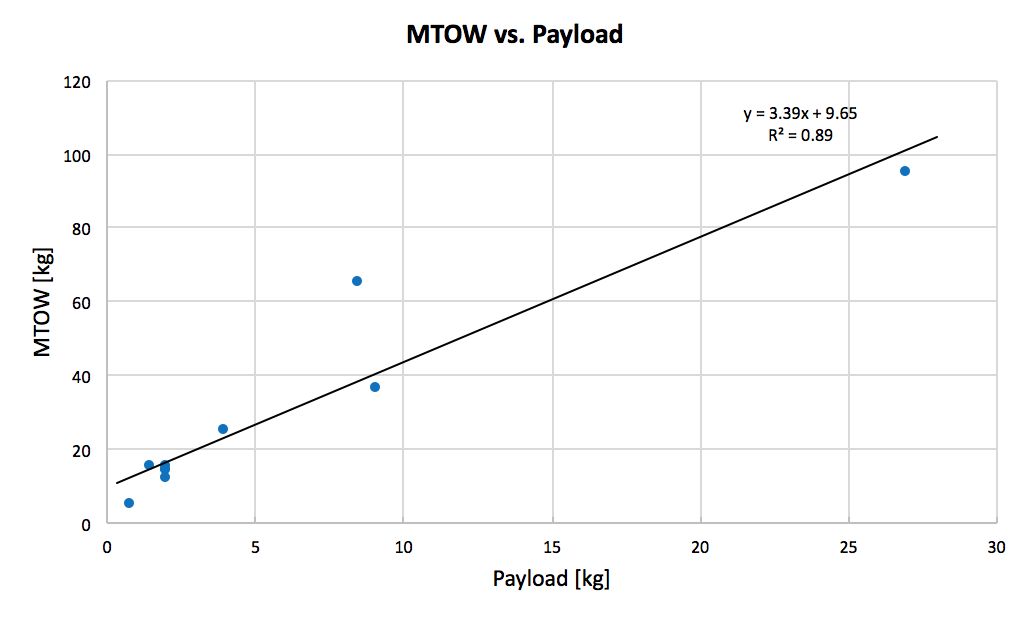
\includegraphics[width = 0.75\textwidth]{PerformanceAnalysis/Figures/MTOW_vs_PL_WQ.png}
\caption{Graph of MTOW vs. Payload Mass}
\end{figure}

The references can be found in \autoref{sec:refvoorgev}. From the graph, a linear relationship between MTOW and payload mass can be identified. The R$^2$ of this trend line is approximately 0.89, signifying a sufficiently good fit. Using the equation of the trend line, a payload mass of 10 kg results in an estimated MTOW of 44 kg.

\subsection{Summary of Mass Estimation}
The estimated MTOWs were all developed based on reference aircraft by comparing the MTOWs to the payloads carried. The MTOWs of the five concepts capable of carrying a payload of 10 kg are summarised in \autoref{tab:mass_summ}. 

\begin{table}[htb]
\centering
\caption{Table of Mass Estimates for Each Concept}
\label{tab:mass_summ}
    \begin{tabular}{lc}
        \toprule
            \textbf{Concept}           & \textbf{MTOW [kg]}\\ \midrule
         The Tailsitter       & 55 \\ \hdashline
         The Tandem           & 58 \\ \hdashline
         The Prandtl-Box      & 38   \\ \hdashline
         The Tiltrotor        & 66 \\ \hdashline
         The Winged Quad.     & 44 \\ \bottomrule
    \end{tabular}
\end{table}

\section{Geometric Properties}
\label{sec:geom_prop}

For the further analysis of the different designs, a preliminary estimation of the geometric properties is required, namely the Aspect Ratio (AR), the Oswald factor (e), and the zero-lift drag coefficient ($C_{D_{0}}$). Where possible, the parameters are roughly estimated from the sketches created in \autoref{ch:concepts}. Although more reliable values are needed for later stages of the design phase, initial estimations are adequate for relative comparisons between the five concepts. 

\subsection{Aspect Ratio}
\label{sec:aspe_rati}

The aspect ratio of each concept has to be estimated in order to perform a preliminary performance analysis. As most of the dimensional properties of the concepts are not known yet at this stage of the design, a preliminary aspect ratio estimation is performed using the sketches created in \autoref{ch:concepts} and in the previous report \cite{baseline}.

Starting with The Winged Quadcopter, an AR of 8 is approximated based on visual inspection of the preliminary sketch.
For the tilt-rotor concept, an aspect ratio of 5.5 is obtained by inspection. This value is also verified by comparing it to the V-22 aspect ratio.
For The Tandem, inspecting the preliminary sketches gives a final aspect ratio of 6.5. The smaller aspect ratio comes from the fact that two wings are used for the production of lift instead of one. As they need around the same amount of surface area, the wingspan can decrease and hence it has a smaller aspect ratio. Using the same reasoning, The Prandtl Box would also receive an aspect ratio of 6.5. However, the vertical wing segments are also included in the calculations of the wingspan and hence The Prandtl Box will receive an aspect ratio of 7.
Finally, The Tailsitter uses nearly its whole surface area for lift, hence a low wingspan is required. This will reduce the aspect ratio considerably. From the sketch in \autoref{ch:concepts} an AR of 4.5 is estimated for The Tailsitter. \autoref{tab:AR} gives an overview of the used aspect ratios for the performance trade-off.

\begin{table}[htb]
    \centering
    \caption{Preliminary Aspect Ratios for All Concepts}
    \label{tab:AR}
    \begin{tabularx}{0.5\textwidth}{lc}
        \toprule
        \textbf{Concept} & \textbf{Aspect Ratio [-]} \\
        \midrule
        The Tailsitter          & 4.5 \\ \hdashline
        The Tandem              & 6.5 \\ \hdashline
        The Prandtl Box         & 7  \\ \hdashline
        The Tiltrotor           & 5.5   \\ \hdashline
        The Winged Quad.        & 8 \\\bottomrule
    \end{tabularx}
\end{table}

\subsection{Oswald Factor}

With exception of The Prandtl Box concept, the Oswald factor of all the concepts is taken to be equal to 0.8, which is the typical value for remote controlled model aircraft \cite{drag_ch3}. The variation of the Oswald factor between the four concepts is small ($\pm$5\%), thus it will have a negligible influence on the change in performance per concept. In addition, the errors caused by the assumptions in the other estimations will most likely be greater than the contribution of the Oswald factor to the change in performance, more so enforcing a constant Oswald factor.

For the Prandtl wing box however, the Oswald factor will be significantly different. According to a Stanford research paper on non-planar wings \cite{Oswald}, the Oswald factor can be estimated to be 1.31. A Prandtl box has a quasi-closed C-wing structure, that includes small vertical wing segments. The dimension of the vertical wing segment strongly influences the Oswald efficiency factor; the greater this segment, the higher the Oswald factor. However, our concept will have a limited vertical wing segment. That is why the corresponding Oswald efficiency factor will have a value of 1.31. 

\subsection{Zero-Lift Drag Coefficient}
\label{sec:zeroliftdrag}

The zero-lift drag coefficient ($C_{D_{0}}$) originates from parasitic drag mainly dependent on the geometry of an aircraft. Therefore, in order to estimate $C_{D_{0}}$ it is sensible to divide an aircraft into geometrical groups making it possible to analyse the different concepts in a structured manner. In this analysis the concepts are divided into fuselage, wing and tail groups.

The analysis consists of determining the amount of fuselages, wings and tails for each concept based on the sketches shown in \autoref{sec:chosconc}. A reference UAV is considered first, which comprises one fuselage, one pair of wings, and one tail. All concepts are compared to this reference UAV.

The Tailsitter concept has no fuselage (it is incorporated into the main wing), one pair of wings, and half a tail, since it only has a vertical fin. The horizontal fin is already incorporated into the main wing, hence the contribution of the tail to the parasitic drag is halved. The Tandem concept has one fuselage, two pairs of wings and no tail. The Prandtl Box concept has one fuselage, two pairs of wings and again only half a tail for the same reason as the Tailsitter concept. The Tiltrotor and Winged Quadcopter concepts each have one fuselage, one pair of wings and one tail. Therefore their configuration is considered identical to the reference aircraft in this analysis.

The contribution of the fuselage, wing and tail groups to the $C_{D_{0}}$ is typically 40\%, 40\%, and 20\% respectively \cite{drag_ch3}. Using this weighting, it is possible to estimate the zero-lift drag coefficient for each concept relative to the reference aircraft. This is done per concept by multiplying the amount of fuselages, wings, and tails determined in the previous paragraph by the corresponding percentage weight, and summing the results.

The final step is to set the absolute value for the $C_{D_{0}}$ of the reference UAV to 0.035, a value typical for remote controlled aircraft \cite{drag_ch3}. It is now possible to estimate the absolute value for the $C_{D_{0}}$ per concept by multiplying the summed relative zero-lift drag by the reference zero-lift drag coefficient. The results of this analysis are summarised in \autoref{tab:cd0estimation}.

\begin{table}[h]
    \centering
    \caption{$C_{D_0}$ Approximation}
    \label{tab:cd0estimation}
    \begin{tabular}{lccccc}
        \toprule
        \textbf{Concept}      & \textbf{Fuselage} & \textbf{Wing} & \textbf{Tail} & \textbf{Total [\%]} & \textbf{$C_{D_0}$ [-]} \\\midrule
        Reference UAV         & 1                         & 1                     & 1                     & 100                 & 0.035          \\\hdashline
        The Tailsitter        & 0                         & 1                     & 1/2                   & 50                  & 0.0175         \\\hdashline
        The Tandem            & 1                         & 2                     & 0                     & 120                 & 0.042          \\\hdashline
        The Prandtl Box        & 1                         & 2                     & 1/2                   & 130                 & 0.0455         \\\hdashline
        The Tiltrotor        & 1                         & 1                     & 1                     & 100                 & 0.035          \\\hdashline
        The Winged Quad. & 1                         & 1                     & 1                     & 100                 & 0.035 \\\bottomrule
    \end{tabular}
\end{table}

The Prandtl Box and Tandem concepts have the highest $C_{D_{0}}$, whilst The Tailsitter has the lowest. The Tiltrotor and The Winged Quadcopter have a $C_{D_{0}}$ similar to the reference UAV.

\subsection{Airfoil Analysis}


In order to carry out a robust analysis and comparison, a temporary airfoil is selected that is the same for all the concepts. Although the chosen airfoil might not be necessarily the most optimal profile for each concept, the chosen airfoil can be regarded as a feasible option for the concepts.

In order minimise the drag, the thickness of the airfoil is preferred to be as low as possible. However, from structural point of view, some concepts are geometrically constrained. For instance, The Tiltrotor concept needs a relatively higher $\frac{t}{c}$ ratio than other concepts. Because the heavy engines and rotating mechanisms on the wing tips require a certain load bearing capacity. This requires the wing to have a minimum thickness; going lower than a certain thickness will drastically increase the weight due to the necessity of adding excessive amounts of material to the structure. For this reason, The Tiltrotor concept is regarded as the most critical in wing loading and root bending moment. Hence, if the chosen airfoil is feasible in this concept, it can be regarded as feasible for the other concepts as well.
The temporary airfoil is selected in an iterative way. First an initial airfoil of the NACA 5-digit family is assumed, then a structural check is performed to see if this airfoil is sufficient to meet the load bearing requirements. This is done by estimating the root moment using moment bending theory. Required thickness dimensions are generated and if these are not able to carry the bending moment, a thicker airfoil will be generated. 
%NEED SOME QUALITY BULLSHIT-JUSTIFICATION ABOUT 15% THICKNESS BEING ENOUGH FOR WITHSTANDING ENGINE LOADS, ETC

% NACA 23015 has both a number of advantageous and adverse properties. First, this profile has a drag bucket, which means that the wing design can be optimised such that the wing induces less drag in certain operations like cruise flight .\cite[p.~37]{aero_vstol}\cite{naca_series} On the other hand, the airfoil has induces high drag when operating outside of the drag bucket operational region.

The chosen NACA 23015 airfoil has a relatively high maximum $C_{L}$ value, which is beneficial for minimising the surface area. It also has a lower aerodynamics moment, which is good for manoeuvrability, but requires extra control effort with regard to stability. 

Reynolds number is approximated to be $3.0*10^{5}$, given the density and air viscosity on sea level, 15 m/s stall velocity and an estimated chord width of 0.3m.

\begin{figure}[htb]
    \centering
    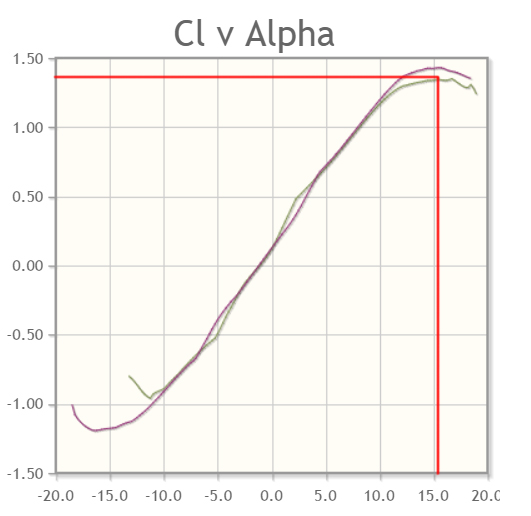
\includegraphics[width=.475\textwidth]{PerformanceAnalysis/Figures/clplot.jpg}
    \caption{Lift Coefficient Alpha Curve of The NACA 23015 Airfoil}
    \label{fig:NACA23015}
\end{figure}

The $C_{L}$ - $\alpha$ plot in \autoref{fig:NACA23015}\footnote{\url{http://airfoiltools.com/airfoil/details?airfoil=naca23015-il}, Accessed 24-05-2017} shows that for the Reynolds number of $3.0*10^{5}$, the $C_{L}$ will have a value of approximately 1.4. The two lines shown in the $C_{L}$ - $\alpha$ plot have Reynolds number of 200,000 and 500,000 each. 

\nomenclature[G]{$\alpha$}{Angle of Attack \nomunit{-}}


\subsection{Wing Loading}
An important parameter in the conceptual sizing of an aircraft is the wing loading. It is the ratio of the weight of the aircraft to the area of the reference wing \cite{aircraft_design}. It can be used to obtain a preliminary estimation of the wing surface area of each design providing a mass estimate is already made.
The driving flight condition for the sizing of the wing surface is when transitioning from the vertical to horizontal flight and vice versa. During this transition the UAV is required to fly at its stall speed which results in the lowest wing loading and hence the largest required wing surface area.

As explained in the previous chapter, the same airfoil is used during the trade-off for each design. In addition, the assumption is made that the stall speed of each design is  20 m/s. This speed was established by looking at reference UAVs and determining a rough ratio between maximum achievable speed and stall speeds. Analysis of different UAVs capable of flying at around 200 km/h has shown that this is a reasonable estimate. The stall speed is purposely chosen to be quite high, as importance is given to high speed flight which requires, as a general rule, less effective surface area. 

As the same airfoil is chosen and stall speed is set to be constant for all five concepts, from \autoref{eq:loading} it can be seen that the surface area, S, only varies with changes in the weight of the aircraft, W.

\begin{equation}
    \frac{W}{S}=\frac{1}{2} \cdot \rho \cdot V_{stall}^{2} \cdot C_{L_{max}}
    \label{eq:loading}
\end{equation}

Once the wing loading is calculated the surface area can be obtained by dividing the weights of the various concepts estimated in \autoref{sec:mass_esti} by the wing loading as shown in \autoref{eq:area}. The wingspan, b, and average chord, $\bar{c}$, can be calculated using \autoref{eq:wingspan} and \autoref{eq:chord} respectively and with the aspect ratios, A, presented in \autoref{sec:aspe_rati}. 

\nomenclature[B]{b}{Wing span \nomunit{m}}
\nomenclature[B]{$\bar{c}$}{Average chord \nomunit{m}}
\nomenclature[B]{A}{Aspect ratio \nomunit{-}}

\begin{minipage}{0.33\textwidth}
    \begin{equation}
        S = \frac{W}{\frac{W}{S}}
        \label{eq:area}
    \end{equation}
    \end{minipage}%
    \begin{minipage}{0.33\textwidth}
    \begin{equation}
        b =\sqrt{A \cdot S}
        \label{eq:wingspan}
    \end{equation}
    \end{minipage}%
    \begin{minipage}{0.33\textwidth}
    \begin{equation}
        \bar{c} = \frac{b}{A}
        \label{eq:chord}
    \end{equation}
\end{minipage}

The geometric properties of the wings of the five concepts are presented in \autoref{tab:wing_summ}.

\begin{table}[htb]
    \centering
    \caption{Table of Geometric Parameters of The Wings of The Five Concepts}
    \label{tab:wing_summ}
    \begin{tabularx}{\textwidth}{p{0.3\textwidth}p{0.2\textwidth}p{0.1\textwidth}p{0.15\textwidth}p{0.1\textwidth}}
        \toprule
        \textbf{Concept} & \textbf{W/S [kg/m$^2$]}  & \textbf{S [m$^2$]} & \textbf{b [m]} & \textbf{c [m]}\\\midrule
        The Tailsitter          &34.58                      & 1.50       & 2.60 & 0.58
        \\ \hdashline
        The Tandem              &34.58                      & 2.31       & 2.74 (ea.) & 0.42
        \\ \hdashline
        The Prandtl Box         &34.58                      & 1.88       & 2.57 & 0.37
        \\ \hdashline
        The Tiltrotor          &34.58                      & 2.17       & 3.45 & 0.63
        \\ \hdashline
        The Winged Quad.   &34.58                      & 1.27       & 3.19 & 0.40 \\\bottomrule
    \end{tabularx}
\end{table}

\nomenclature[B]{W/S}{Wing loading \nomunit{kg/m$^2$}}
\nomenclature[B]{S}{Wing surface area \nomunit{m$^2$}}

\section{Performance Criteria}
\label{sec:perf}

In this section, the different performance criteria used in the trade-off are analysed. From requirements \textbf{SYS-PF-1.3}, \textbf{SYS-PF-1.4} and \textbf{SYS-PF-2.3}, it has been deduced that the most important parameters regarding performance are the range, the endurance and the required power for the UAV. Other performance specific properties like drag and mass are included in these calculations.  
First, the endurance analysis is presented in \autoref{sec:endu_ana}\begin{comment}No autoref on purpose here \end{comment}%
. Then, in \autoref{sec:range_ana}\begin{comment}No autoref on purpose here \end{comment}%
, a preliminary range difference between the different concepts in calculated and finally, in \autoref{sec:power_ana}\begin{comment}No autoref on purpose here \end{comment}%
, the required power for different cases is obtained.

\subsection{Endurance Analysis}
\label{sec:endu_ana}

In this section, the maximum endurance of each concept is analysed. It is assumed that the drone is flying at an optimal flight condition for maximum endurance. Neither take-off and landing nor any other flight condition are included in the calculations of this analysis.

To calculate the maximum endurance of each concept, the optimum lift coefficient of each concept has to be calculated. This is achieved using \autoref{eq:lift_end}, derived by minimising the required power.

\begin{equation}
    C_{L_{endu}} = \sqrt{\frac{3\cdot C_{D_0}}{k}} \quad \mathrm{where} \quad k=\frac{1}{\pi \cdot e\cdot A}
    \label{eq:lift_end}
\end{equation}

Then setting the weight equal to the lift gives the optimum velocity for maximum endurance flight.

\begin{equation}
    V_{opt} = \sqrt{\frac{2\cdot W}{\rho\cdot S\cdot C_{L_{opt}}}}
    \label{eq:vopt}
\end{equation}

The maximum endurance is then obtained using \autoref{eq:endurance} \cite{ran_end}.

\begin{equation}
    E = (R\cdot t)^{1-n}\cdot \Bigg{[}\frac{\eta_{tot}\cdot U\cdot C}{\frac{1}{2}\cdot\rho \cdot V_{opt}^3\cdot S\cdot C_{D_0} + \frac{2\cdot W^2\cdot k}{\rho\cdot V_{opt}\cdot S}}\Bigg{]}^n
    \label{eq:endurance}
\end{equation}

For further analysis, efficiency factors are assumed to be equal to one. This means $\eta_{tot}=1$, $(R\cdot t)=1$ and $n=1$. Then, as the energy $U\cdot C$ depends on the type and mass of energy source, a preliminary energy estimation can to be done for the performance calculation. As a first order estimation it is assumed that the battery used is of the Lithium-Ion type, having an average energy density of 135 $\frac{W\cdot h}{kg}$. They are used for their high energy density compared to other available battery types. Disadvantages however are a higher cost and the need of a robust protection to ensure reliability. Using a preliminary battery mass estimation of 2 kg, an energy of 270 $W\cdot h$. Care should be taken to not confuse the estimated values of the endurance with the actual endurance the design can achieve. Although acceptable assumptions have been made for all of the variables, it is not possible yet to accurately obtain the properties at this stage of the design process. Furthermore, required amount of energy and hence battery mass depends on each design. In order to perform a fair trade-off, each design is assumed to have the same battery mass. Because the same methods have been applied for the generation of all the variables, the relative difference between the endurance values is still acceptable and can thus be used for the trade-off. \autoref{tab:trade_endu} gives a general overview of the endurance of each concept. The endurance is expressed in hours and in a percentage. The percentage value is the percentage of the endurance of the concept with respect to the average of all the concepts, as explained in \autoref{sec:grading_sys_perf}.

\begin{equation}
    E =  \frac{U\cdot C}{\frac{1}{2}\cdot \rho\cdot V_{opt}^3\cdot S\cdot C_{D_0} + \frac{2\cdot W^2\cdot k}{\rho \cdot V_{opt}\cdot S}}
    \label{eq:endurance_simpl}
\end{equation}

\begin{table}[htb]
    \centering
    \caption{Overview of Endurance Ranking for Each Concept}
    \label{tab:trade_endu}
    \begin{adjustbox}{width=1\textwidth}
    \small
        \begin{tabular}{lcccc}
        \toprule
        \textbf{Concept} & \textbf{Weight [N]} & \textbf{Aspect Ratio [-]} & \textbf{V$_{Endurance}$ [m/s] }& \textbf{Endurance [\%], [hrs]} \\ \midrule
        The Tailsitter          &540   &4.5 &24  & 78, 0.23\\\hdashline
        The Tandem              &569   &6.5 & 17 & 82, 0.24\\\hdashline
        The Prandtl Box         &373   &7  & 14& 168, 0.50\\\hdashline
        The Tiltrotor           &647   &5.5   & 20 & 60, 0.18\\\hdashline
        The Winged Quad.        &431   &8   &20 & 112, 0.33\\\bottomrule
        \end{tabular}
        \end{adjustbox}
\end{table}



\subsection{Range Analysis}
\label{sec:range_ana}
In this section, the range of each concept is calculated. For this, it is assumed that the drone is performing a simple mission of only trying to achieve maximum distance. Neither take-off \& landing nor any other mission related phase are included in these calculations. 

The range analysis is performed similarly to the endurance analysis. The only difference lies in the flight condition for maximum range. The lift coefficient is approximated using \autoref{eq:lift_ran}, derived by maximising the lift over drag ratio. 

\begin{equation}
    C_{L_{range}} = \sqrt{\frac{C_{D_0}}{k}} \quad where \quad k=\frac{1}{\pi\cdot e\cdot A}
    \label{eq:lift_ran}
\end{equation}

The optimal velocity for maximum range can again be calculated using \autoref{eq:vopt}. Then the endurance at maximum range conditions is obtained using \autoref{eq:endurance_simpl} and finally using \autoref{eq:range} the range is calculated.

\begin{equation}
    R = E\cdot V_{range}
    \label{eq:range}
\end{equation}

In \autoref{tab:trade_range} the range for each of the concepts is shown. The trade-off ranking can also be seen for each concept. As with the endurance ranking, the absolute values in the Table of low accuracy and they will thus only be used for the ranking of the designs due to their relative difference. 

\begin{table}[H]
    \centering
    \caption{Overview of Range Ranking for Each Concept}
    \label{tab:trade_range}
    \begin{adjustbox}{width=1\textwidth}
    \small
        \begin{tabular}{lcccc}
        \toprule
        \textbf{Concept} & \textbf{Weight [N]} & \textbf{Aspect Ratio [-]} & \textbf{V$_{range}$ [m/s] } &\textbf{Range [\%],[km]}  \\ \midrule
        The Tailsitter           &540 &4.5& 32  & 104, 23\\\hdashline
        The Tandem               &569 &6.5& 22   & 77, 17\\\hdashline
        The Prandtl Box          &373 &7 & 18 & 129, 29\\\hdashline
        The Tiltrotor            &647 &5.5  &27 & 68, 15\\\hdashline
        The Winged Quad.         &431 &8  &25.7 &123, 27 \\\bottomrule
        \end{tabular}
        \end{adjustbox}
\end{table}


\subsection{Power Analysis}
\label{sec:power_ana}

In order to assess whether each of the five concepts can meet the challenging requirements derived from the various stakeholder needs, an analysis on the power required for the various flight phases is necessary. The power required to hover and climb vertically will therefore be calculated for the five concepts and compared. Later on the power required for climb during the horizontal flight phase will be calculated.


\subsubsection{Vertical Flight Phase}
During vertical flight the engines/rotors needs to overcome the weight of the UAV, i.e. the thrust to weight ratio must be greater than one ($\frac{T}{W} \ge 1$). The required power for both hovering and vertical climb will therefore be analysed.

\subsubsection*{Power Required to Hover}
During hovering, since the vertical velocity is zero, thrust is generated by accelerating air from zero velocity from all directions through the rotor disk. Employing the conservation of both energy and momentum, the power required to hover can be expressed as a function of weight and is characterised by \autoref{eq:powe_requ_hove} below\footnote{\url{http://s6.aeromech.usyd.edu.au/aerodynamics/index.php/sample-page/aircraft-performance/hoverclimbdescent-analysis/}, Accessed 18-05-2017}.

\begin{equation}
\label{eq:powe_requ_hove}
\begin{split}
  P_{req} &= W \cdot v_{\imath} \qquad \mathrm{where,} \quad v_{\imath} = \sqrt{\frac{(T = W)}{2 \cdot \rho \cdot A}}\\
\Rightarrow  P_{req} &= \sqrt{\frac{W^3}{2 \cdot \rho \cdot A}}
\end{split}
\end{equation}

\nomenclature[B]{$P_{req}$}{Power required \nomunit{kW}}
\nomenclature[B]{$W$}{Weight \nomunit{N}}
\nomenclature[B]{$v_{\imath}$}{Induced velocity at rotor disk \nomunit{m/s}}

The power required to hover is therefore proportional to the square root of weight cubed, i.e. $P \propto W^{\frac{3}{2}}$ and it is therefore clear that the lighter the UAV is, the less power is required to hover. The concepts are therefore ranked from lowest to highest required power.

\subsubsection*{Power Required to Climb}

During a vertical climb at a constant velocity the air flow through the rotor already has momentum. This changes the required power to maintain such a climb as the induced velocity is now different. The power required for vertical climbing flight is given by \autoref{eq:powe_requ_clim}. It is important to note that if the climb rates are small, thrust and weight can be considered equal (i.e. $T = W$).

\begin{equation}
\label{eq:powe_requ_clim}
\begin{split}
  P_{req} &= W \cdot v_{\imath} \qquad \mathrm{where,} \quad v_{\imath} = \frac{V_{c}}{2} + \sqrt{ \left( \frac{V_{c}}{2} \right) ^2 + \frac{(T = W)}{2 \rho A}}\\
  \Rightarrow P_{req} &= W \left( \frac{V_{c}}{2} + \sqrt{ \left( \frac{V_{c}}{2} \right) ^2 + \frac{W}{2 \rho A}} \right)
\end{split}
\end{equation}

As the vertical climb rate is set to a constant value of 4 m/s as stipulated by requirement \textbf{SYS-PF-2.4} it is clear that the required power increases with increasing weight. As can be seen in \autoref{eq:powe_requ_clim} the drag is not included.This if for two reasons, firstly preliminary calculations show that they are in the order of 10 N for the prescribed climb rate and secondly the goal of this analysis is primarily to determine how much power each concept requires relative to the others.

\subsubsection{Disk Loading}

In order to evaluate the power equations presented above (namely Equations \ref{eq:powe_requ_hove} \& \ref{eq:powe_requ_clim}) the area of the rotor disk, A is required. By obtaining a value for the disk loading, (W/A) of the five concepts coupled with knowing the mass estimate of each concept, the rotor disk area can be calculated ($A = \frac{W}{(W/A)}$).

From the graph presented in \autoref{fig:MTOW_vs_disk_load} a relationship was established between the MTOW and the disk loading.

\begin{figure}[H]
\centering
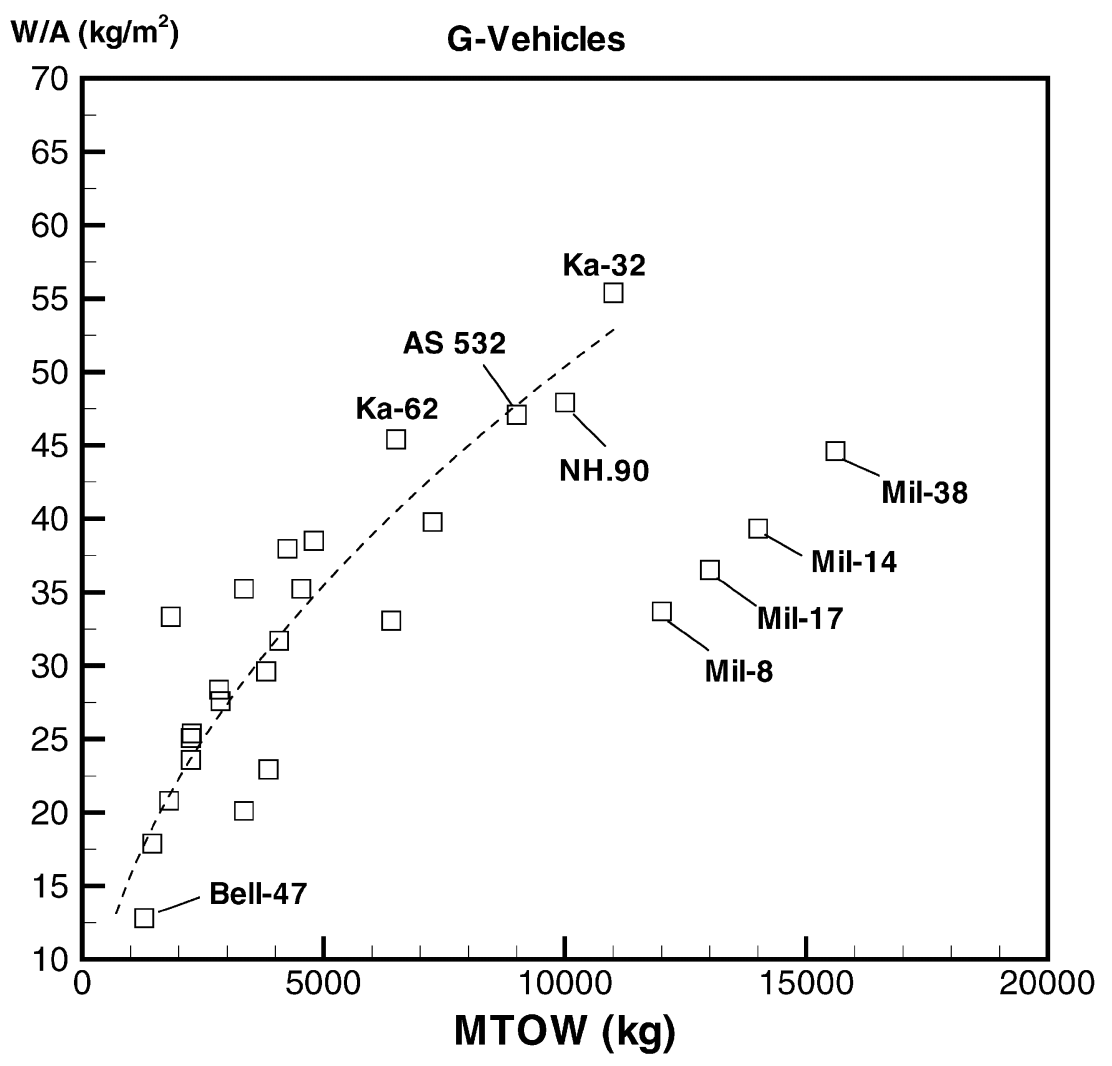
\includegraphics[width=0.75\textwidth]{PerformanceAnalysis/Figures/DiskLoading_vs_MTOW.png}
\caption{Graph of Disk Loading Versus MTOW \cite{diskloading}}
\label{fig:MTOW_vs_disk_load}
\end{figure}

The disk loading can be approximated as a linear function of MTOW and is expressed as in \autoref{eq:disk_load}. 

\begin{equation}
\label{eq:disk_load}
(W/A) = 0.0031 \cdot MTOW + 15.03
\end{equation}



\subsubsection{Power Required for Maximum Velocity}

The maximum power required during horizontal flight is achieved at maximum velocity, that is at 200 km/h (55.6 m/s) as stipulated by requirement \textbf{SYS-PF-1.2}. The power required is defined by \autoref{eq:PR}.

\begin{equation}
    P_{r} = C_D\cdot \frac{1}{2}\cdot\rho \cdot V^3\cdot S
    \label{eq:PR}
\end{equation}

The drag coefficient is calculated in \autoref{eq:cd}, where the zero lift drag coefficient is obtained in \autoref{sec:zeroliftdrag} and the lift coefficient is calculated using \autoref{eq:liftcoef}. 

\begin{equation}
    C_L = \frac{2\cdot W}{\rho \cdot V^2\cdot S}
    \label{eq:liftcoef}
\end{equation}

\begin{equation}
    C_D = C_{D_0} + \frac{C_L^2}{\pi \cdot e\cdot A}
    \label{eq:cd}
\end{equation}

The results for each concept are summarised in \autoref{tab:powe_requ_hove}.

\subsubsection{Summary}

Having established the calculation for the power required in the three most important cases, namely maximum velocity, hovering and climbing, the concepts can be ranked for the trade-off. \autoref{tab:powe_requ_hove} illustrates each concept and their different required powers. Then, the maximum of these values is used for the trade-off. As for each concept this value will drive the design of the propulsion subsystem. The maximum P$_{req}$ is also given as a percentage value with respect to the average of all the maxima.

\begin{table}[H]
\centering
\caption{Table Ranking Concepts Based On Power Required}
\label{tab:powe_requ_hove}
\begin{tabular}{p{3.5cm} >{\centering}p{2.6cm} >{\centering}p{2.6cm} p{2.6cm}<{\centering} p{2.4cm}<{\centering}}
\toprule
 \textbf{Concept}  & \textbf{P$_{req}$ for max velocity [kW]}    & \textbf{P$_{req}$ to hover [kW]}  & \textbf{P$_{req}$ to climb [kW]} & \textbf{Max P$_{req}$ [\%],[kW]}
\\ \midrule
 The Tailsitter    &        2.8                     &  4.2                   & 5.5   &  74,5.5 \\ \hdashline
 The Tandem        &        10.2                   &  5.0                   & 6.4   & 136,10.2 \\\hdashline
 The Prandtl-Box   &        9.0                   &  2.9                    &3.8  & 120,9.0\\ \hdashline
 The Tiltrotor     &              8.0                &  5.1                   & 6.4  & 107,8.0 \\ \hdashline
 The Winged Quad.  &                  4.7            &  3.4                    &4.4  & 63,4.7 \\ \bottomrule
\end{tabular}
\end{table}







    \chapter{Stability \& Control}
\label{sec:manostab}

Regardless of performance characteristics, controlling the vehicle is of vital importance to any mission at any phase. For the aircraft under consideration, the controllability is absolutely crucial in both vertical and in horizontal flight. Horizontal flight phases for this particular vehicle are associated with high velocities at low altitudes, which requires very precise control of the UAV. Vertical flight phases are associated with taking off and landing on small landing sites possibly in an urban environment. In this condition the allowed attitude and positional errors are expected to be very limited. In order to ensure that these aspects are sufficiently and correctly represented in the selection process, all concepts are analysed for manoeuvrability, stability and controllability in this chapter. First, the results of this analysis are summarised in \autoref{sec:sum}. Then, the general approaches for judging  manoeuvrability, stability and controllability as well as the assigned weights are explained in \autoref{sec:app}. Finally, the reasoning behind each rating is explained in more detail per sub criterion and per concept in \autoref{sec:ca}.

\section{Summary}
\label{sec:sum}

The final result of the analysis performed in this chapter is summarised in \autoref{tab:controlsubtrade}:

\begin{table}[H]
    \centering
    \caption{MSC Sub Trade-off}
    \label{tab:controlsubtrade}
    \begin{tabular}{r|>{\centering}p{4cm}:>{\centering}p{3.5cm}:>{\centering}p{2.5cm}|c}
    \textbf{Concept \rotatebox{90}{\hspace{0.5cm}Criterion}}    & 
    \rotatebox{90}{\textbf{Controllability}}                      &
    \rotatebox{90}{\textbf{Stability}}                           & 
    \rotatebox{90}{\textbf{Manoeuvrability}}  &  
    \rotatebox{90}{\textbf{Outcome}}                    
    \\ \midrule
    Tailsitter      & -   & 0   & +   & 46\% 
    \\\hdashline
    Tandem          & 0     & -     & 0      & 41\% 
    \\\hdashline
    Prandtl Box     & 0     &  -   & 0     & 41\% 
    \\\hdashline
    Tiltrotor       &  + +     & +   & -   & 72\% 
    \\\hdashline
    Winged Quad.     & + +    & +     & +    & 85\% 
    \\ \midrule\midrule
    Weight          & 40    & 35    & 25    &  
    \end{tabular}
\end{table}

As can be seen, the highest score was earned by the Winged Quadcopter. It combines good controllability in both horizontal and vertical flight modes with a relatively wide range of allowable CG locations for stability and more manoeuvrability than most other concepts. The Tiltrotor concept earned the second highest score in this sub trade-off. Its score is identical to that of the Winged Quadcopter in both the controllability and stability departments. However, it does score lower on manoeuvrability due to its high moments of inertia about the X and Z axes. These higher moments of inertia can be contributed to the placement of the engines, which both are at the wing tips. The Tailsitter was ranked third with a score of 46.25 \% . The main reasons for this lower score were the relatively limited range of CG positions for stability and the lower control surface effectiveness. In manoeuvrability, the concept performed comparable to the Winged Quadcopter. The Tailsitter is closely followed by the Tandem and Prandtl Box concepts, which both scored 41.25 \%. They both have a limited range of allowable CG positions for stability whilst neither score particularly high in controllability nor in manoeuvrability.

\section{Approach}
\label{sec:app}


\subsection{Reference Frame}

In order to have a consistent axis system throughout the report, the right-handed, body-fixed reference frame $F_b$ was chosen as a basis. It is visualised in \autoref{fig:body_frame}. 

\begin{figure}[htb]
    \centering
    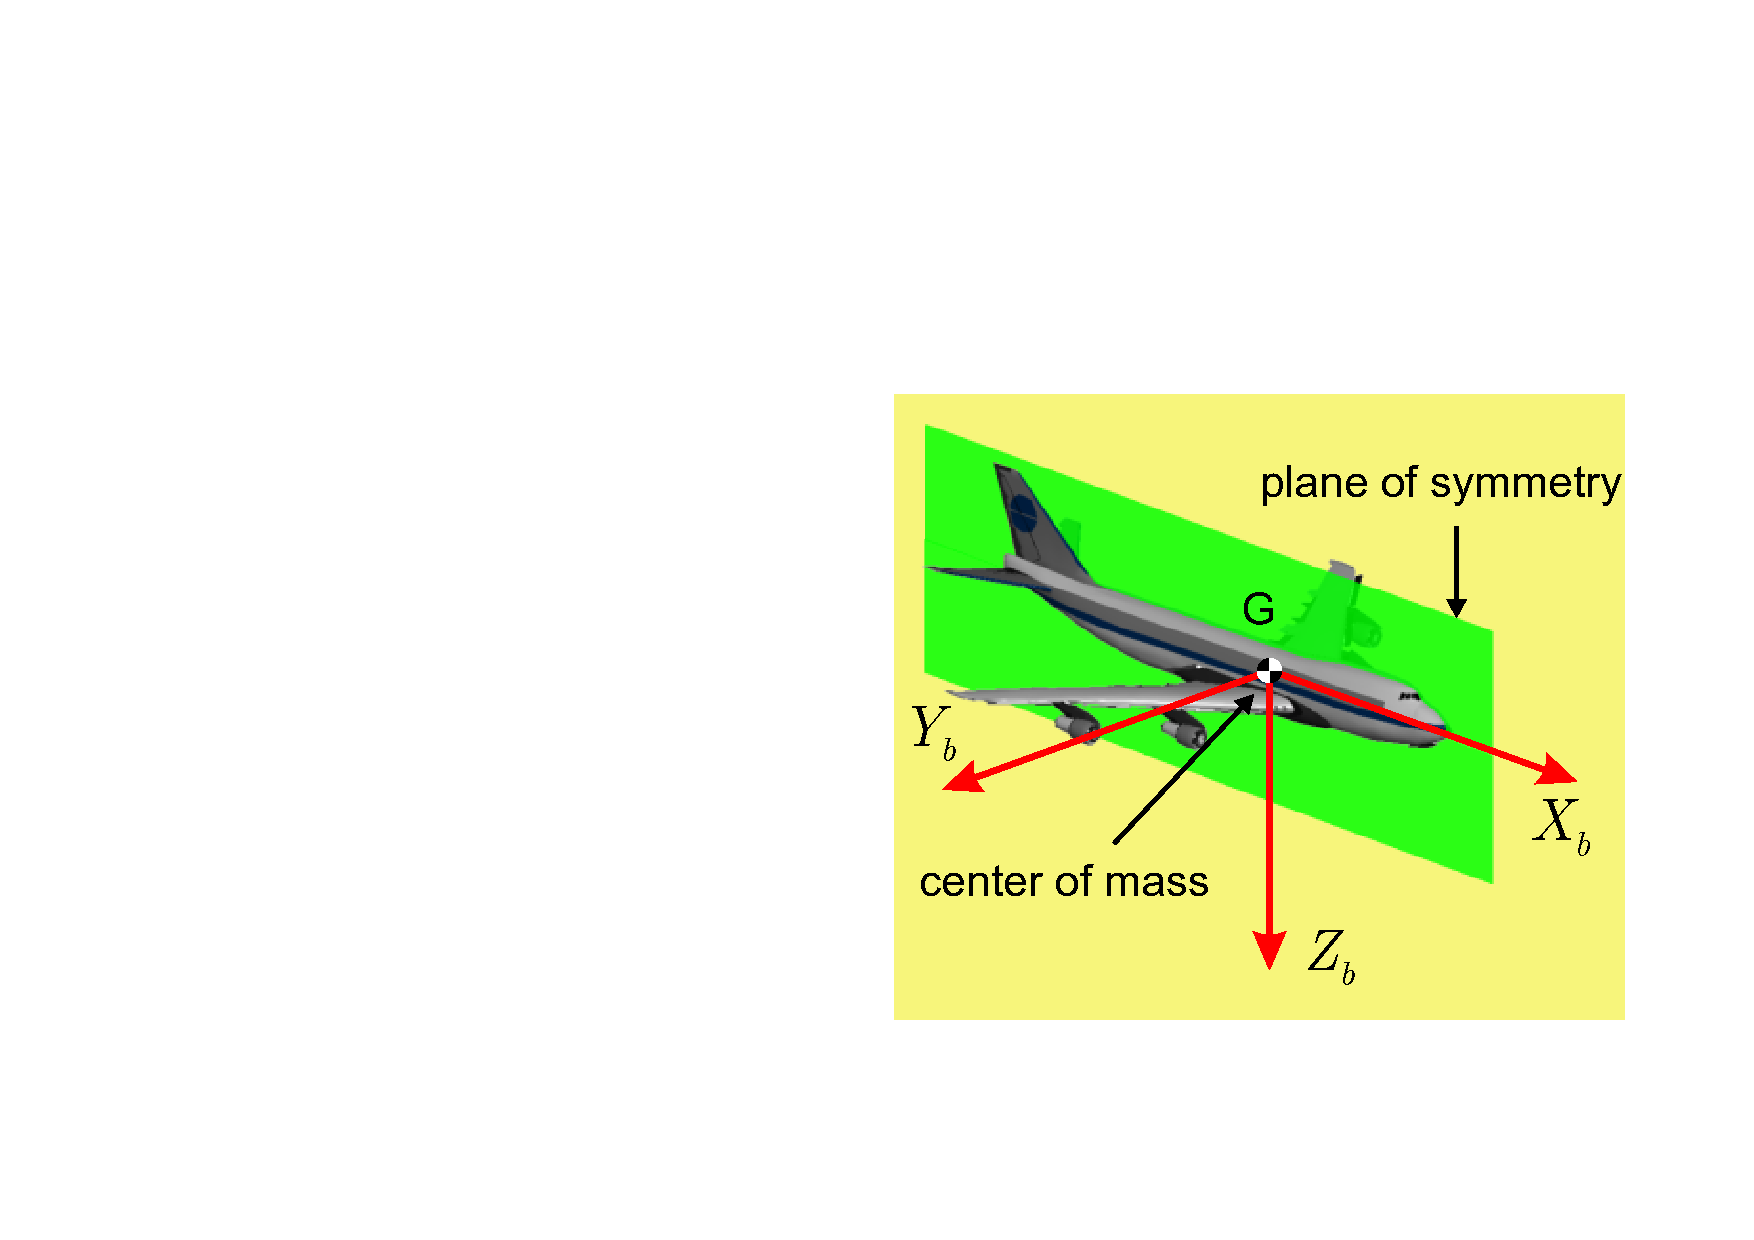
\includegraphics[width=.35\textwidth]{Stability/Figures/body_frame.pdf}
    \caption{Body Fixed Reference Frame \cite{fd_lec08}}
    \label{fig:body_frame}
\end{figure}



\subsection{Stability}

The stability of each concept in both horizontal and vertical flight regimes was investigated based on the sketches available from the Baseline Report \cite{baseline}. For horizontal flight the configurations of the lifting surfaces were evaluated for the change in pitching moment due to a disturbance change in angle of attack. The range of Centre of Gravity (CG) locations for which the aircraft would be longitudinally stable was evaluated per concept. For vertical flight stability, the configuration of the engines is evaluated because none of the concepts employ lifting surfaces in this mode. The definition of the scores can be found below in \autoref{tab:dsr}. 

\begin{table}[H]
\centering
\caption{Definition of Stability Ratings}
\label{tab:dsr}
    \begin{tabular}{llc}
        \toprule
            &\textbf{Rating}           & \textbf{Meaning}
        \\ \midrule
          & ++            & Stable in horizontal and vertical flight for a wide range of CG positions          
        \\ \hdashline
          & +               & Stable for wide CG range in horizontal flight, neutrally stable in vertical flight
        \\ \hdashline
          & 0          & Stable in horizontal flight for limited CG range, stable in vertical flight 
        \\ \hdashline
          & -           & Stable in horizontal flight for limited CG range, neutral stability in vertical flight 
        \\ \hdashline
          & - -   & Unstable in horizontal or vertical flight
        \\ \bottomrule
    \end{tabular}
\end{table}

\subsection{Controllability}

The control systems of the different concepts were analysed for their effectiveness based on the moment arms for various control surfaces and engines as derived from the geometry of the conceptual sketches. The definitions of the ratings are shown in \autoref{tab:dcr}.

\begin{table}[H]
\centering
\caption{Definition of Control Ratings}
\label{tab:dcr}
    \begin{tabular}{llc}
        \toprule
            &\textbf{Rating}           & \textbf{Meaning}
        \\ \midrule
          & ++            &  Effective pitch, roll and yaw control      
        \\ \hdashline
          & +               & Effective pitch control,low roll and yaw control effectiveness
        \\ \hdashline
          & 0          & Average pitch control effectiveness
        \\ \hdashline
          & -           & Low pitch control effectiveness, effective roll control
        \\ \hdashline
          & - -    & Low pitch and roll control effectiveness
        \\ \bottomrule
    \end{tabular}
\end{table}

\subsection{Manoeuvrability}

Next to the control surface effectiveness it is desirable to have a low mass moment of inertia around all three body axes. Even though the Hybrid UAV will be optimised for high-speed cruise conditions, it still needs to be able to roll and pitch up quickly, for instance, to avoid obstacles at low altitudes.

The approach to analysing the moments of inertia was to use the weight and wing size estimations derived in \autoref{ch:perf_analy} to create simplified CATIA models of each concept. Since the knowledge about geometry and component weights is limited at this stage of the project, a number of assumptions are made. The most important ones are listed below:

\begin{itemize}%leave periods in this table -K
    \item All concepts share the same cylindrical fuselage which includes battery and payload.
    \item Engines and propellers can be modelled as a single cylinder and have a constant power-to-weight ratio.
    \item Engine mass is 20\% of total mass (based on a statistical analysis in \cite{Wei_2017}).
    \item Horizontal and vertical tail plane surfaces are 20\% of the main wing area (based on ratios derived from reference aircraft \footnote{\url{https://booksite.elsevier.com/9780340741528/appendices/data-a/table-8/table.htm}}).
    \item Structural mass per unit area is equal for all aerodynamic surfaces.
\end{itemize}

\autoref{fig:prandtl_inertia} shows the model of the Prandtl Box concept to give an impression of the level of accuracy that can be achieved by this analysis. Since the fuselage and payload is assumed to be equal for all five concepts, the main differences in inertia follow from the area and aspect ratio of the wing, mass and placement of the engines and the presence of additional elements such as tailplanes and wing connectors. Even though the absolute value of the result should be handled with care and updated when more reliable dimensions and mass values are available, the distinct configuration of each concept allows for a reasonable comparison. 

\begin{figure}[htb]
    \centering
    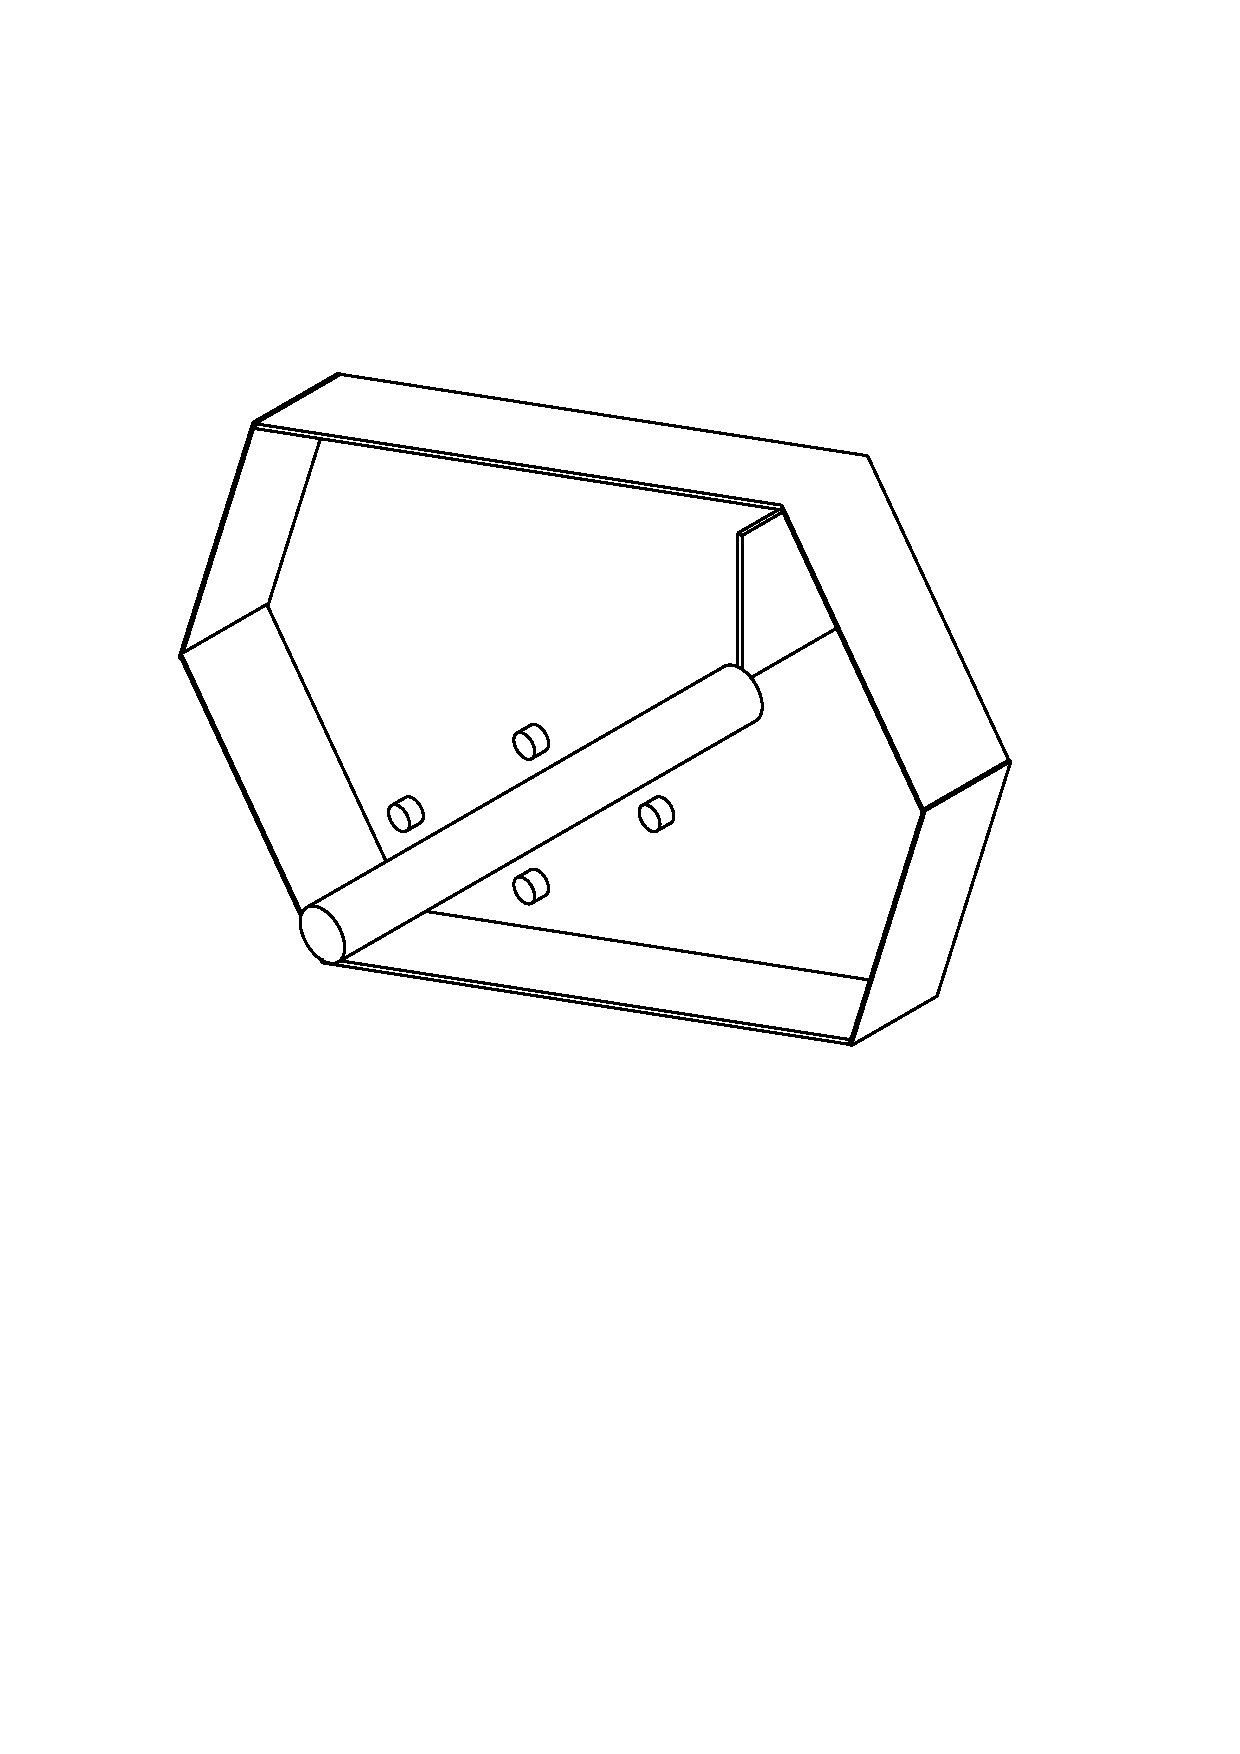
\includegraphics[width=.4\textwidth]{Stability/Figures/prandtl.pdf}
    \caption{Simplified Model of the Prandtl Box Concept}
    \label{fig:prandtl_inertia}
\end{figure}

\autoref{tab:dmr} shows the rating scheme for manoeuvrability, it is derived by doubling the average total inertia of all concepts and then splitting the resulting range into five categories.  

\begin{table}[H]
\centering
\caption{Definition of Manoeuvrability Ratings}
\label{tab:dmr}
    \begin{tabular}{llc}
        \toprule
            &\textbf{Rating}           & \textbf{Total inertia range $[kg \times m^2]$}
        \\ \midrule
          & ++            &  0-30       
        \\ \hdashline
          & +               & 30-60
        \\ \hdashline
          & 0          & 60-90
        \\ \hdashline
          & -           & 90-120
        \\ \hdashline
          & - -    & 120 and more
        \\ \bottomrule
    \end{tabular}
\end{table}

\subsection{Criteria Weights}
In order of increasing importance the sub criteria are as following: manoeuvrability, stability and control. Their weights are determined to be 25, 35 and 40 respectively. Manoeuvrability is assigned the lowest weight out of the three criteria because good manoeuvrability is less vital for the UAV's intended mission. Control is weighted heavier than stability because an effective control system can overcome the undesirable effects of an unstable aircraft, whereas an ineffective control system paired with a very stable aircraft becomes even more of a problem. 

% Oscar: Tailsitter
\section{Concept Analysis}
\label{sec:ca}

All five concepts were analysed for their controllability, stability and manoeuvrability. As was explained in \autoref{sec:app}, the values obtained for moments of inertia are most meaningful in comparison, so a table was added in the beginning. 

\subsection{Overview of Mass Moments of Inertia}

\autoref{tab:inertia_overview} shows the result of the MOI analysis for all concepts. A brief discussion of remarkable values is provided in the concept sections. 

\begin{table}[htb]
    \centering
    \caption{Mass Moments of Inertia for Each Concept in $[kg \times m^2]$ }
    \label{tab:inertia_overview}
    %\begin{adjustbox}{width=1\textwidth}
    \small
        \begin{tabular}{lcccc}
        \toprule
        \textbf{Concept} & \textbf{$I_x$} & \textbf{$I_y$} & \textbf{$I_z$} & \textbf{$I_{total}$} \\ \midrule
        The Tailsitter          &1.9   & 25.3  & 26.6 & 53.7    \\\hdashline
        The Tandem              &10.0  & 27.3  & 36.3 & 73.6    \\\hdashline
        The Prandtl Box         &13.6  & 26.4  & 35.1 & 75.1    \\\hdashline
        The Tiltrotor           &32.7  & 23.5  & 53.9 & 110.1   \\\hdashline
        The Winged Quad.        &4.9   & 20.3  & 24.2 & 49.4    \\\bottomrule
        \end{tabular}
        %\end{adjustbox}
\end{table}

\subsection{The Tailsitter}
\begin{figure}[htb]
    \centering
    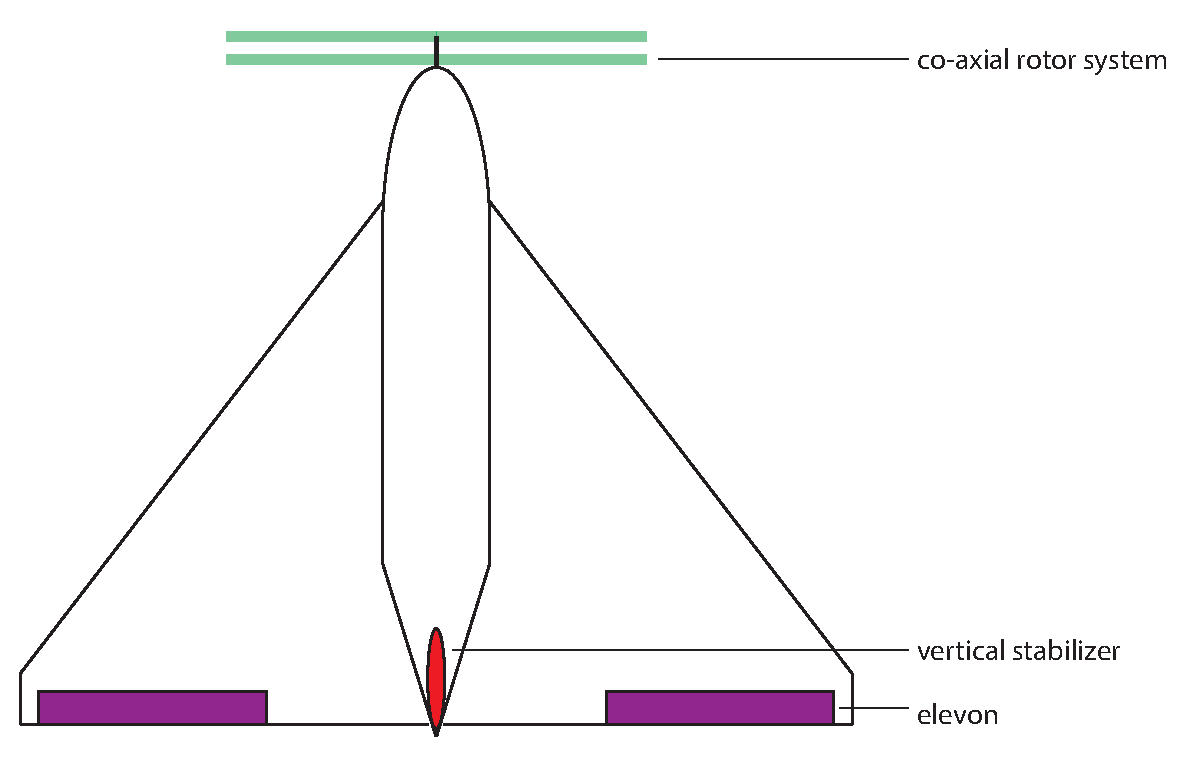
\includegraphics[height=6cm]{Stability/Figures/concept_1.pdf}
    \caption{Control Layout of The Tailsitter.}
    \label{fig:Cts}
\end{figure}
\paragraph{Control}

The layout of the control system for the Tailsitter is depicted in \autoref{fig:Cts}. In vertical flight mode, the attitude of the Tailsitter is fully controlled with the coaxial rotors mounted on the nose of the aircraft. As they are counter rotating, the yaw rate of the vehicle can be controlled by inversely adjusting the angle of attack of both the rotor blades. Additionally, both the pitch and roll rates can be manipulated with cyclic angle of attack increments on both rotors. Finally, the rate of ascent or decent is controlled with collective angle of attack adjustments on both rotors. 

In horizontal flight phases, the coaxial rotors are only used as a means of propulsion. Attitude control is achieved solely by the manipulation of aerodynamic control surfaces. Particularly, a conventional rudder is used for directional control and both longitudinal and lateral control are accomplished with a single set of control surfaces. These elevons are located at the trailing edge of the delta-shaped wing.

Because this design lacks a conventional tail, the aerodynamic control surfaces used to generate the required pitching moments are located closer to the centre of gravity than for conventional aircraft. This means that either larger surfaces or greater deflection angles are required to generate a sufficient pitching moment. Consequently, the trim drag will be higher for this concept than for a standard configuration aircraft. Similarly, the rudder is also located closer to the centre of gravity in this configuration. Hence, for the rudder to be effective, a rather large surface or a significantly larger deflection of this surface are required. This will increase the amount of drag associated with use of the rudder. However, the propellers are mounted on the aircraft's centre line. Therefore, no prolonged rudder deflections are required to balance out a propulsion induced torque in a one engine out scenario. Furthermore, take-off and landing are performed in vertical mode without use of the control surfaces. So, the rudder is not frequently used during flight and its lower efficiency is therefore tolerable. The increased trim drag that is sustained for longitudinal stability might be detrimental to the performance of this design. 


\paragraph{Manoeuvrability}

The Tailsitter is a very promising concept when it comes to manoeuvrability. The engine block and propellers are situated on the centre line of the UAV, meaning that there is no extra inertia term due to axis offsets in y and z direction. In combination with low wing span, this leads to a very low moment of inertia around the roll axis compared to the other concepts. The MOIs around the pitch and yaw axis are average, which is due to the large wing surface and the offset of the engine to the UAV c.g. in x direction. 

\paragraph{Stability}

In vertical flight mode, The Tailsitter is neutrally stable about all three axes. The centre of gravity always lies on the line of action of the thrust force, because of the way the rotors are mounted on the vehicle. Furthermore, the gravitational force vector goes through the centre of gravity by definition. Hence, a disturbance to any equilibrium condition is neither amplified nor restored. The stability could be improved by employing a stabiliser bar, as is quite common in helicopter designs. On the other hand the lack of stability could be overcome with active control such an electronic control unit based on gyroscopic sensors.

During horizontal manoeuvres, the tailless delta wing configuration is not ideal from a stability point of view. The vehicle has only a single lifting surface. Therefore in order to have longitudinal stability, the centre of gravity should be in front of the aerodynamic centre and the moment about the aerodynamic centre should be positive. This imposes some limitations on the weight distribution and wing design. High-camber airfoils or trailing edge high-lift devices contribute to a negative pitching moment about the aerodynamic centre. Their application would therefore adversely affect the stability of the UAV. On the contrary, implementing a wash-out or a reflex cambered airfoil as an example would increase the pitching moment about the aerodynamic centre.

%Oscar: Tandem
\subsection{The Tandem}
\begin{figure}[htb]
    \centering
    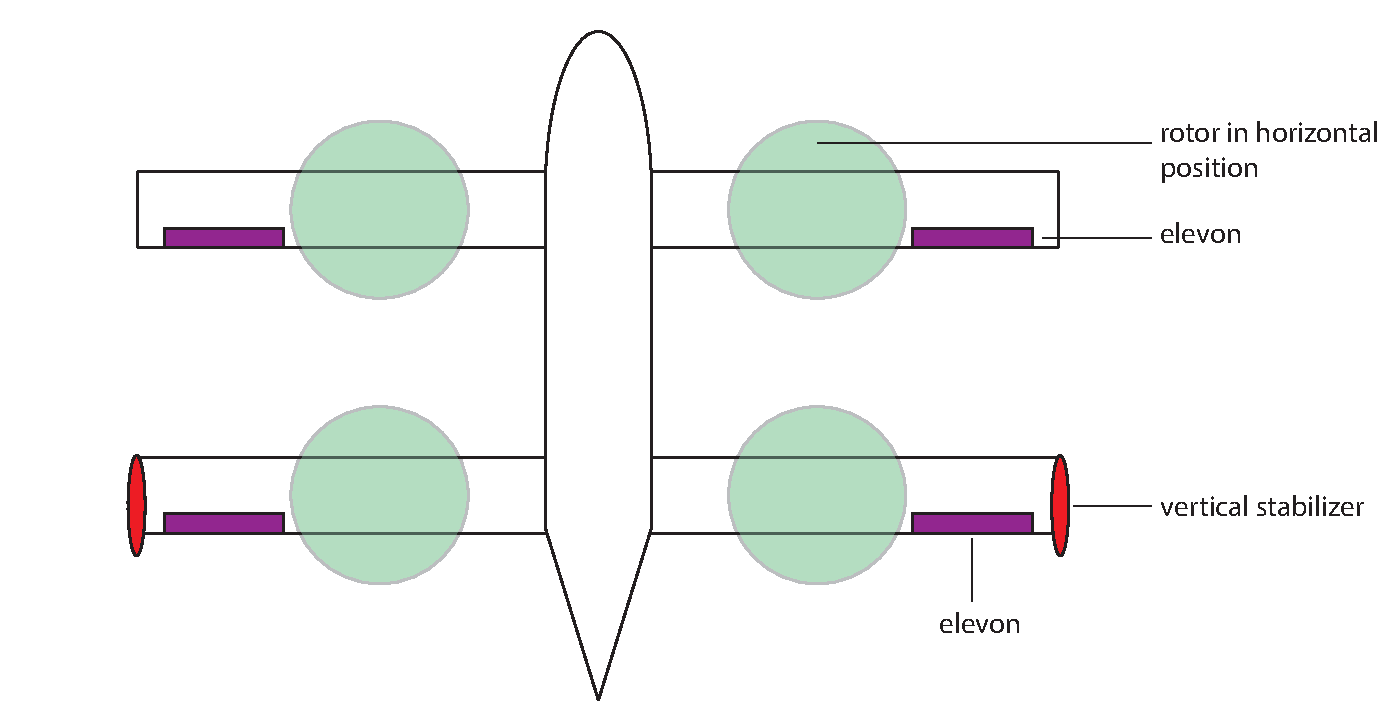
\includegraphics[height=6cm]{Stability/Figures/concept_2.pdf}
    \caption{Control Layout of The Tandem}
    \label{fig:Ctd}
\end{figure}

\paragraph{Control}
During vertical flight phases, The Tandem will be controlled in a similar way to the way conventional quadcopters are controlled. The full layout of the controls is shown in \autoref{fig:Ctd}. A total of four rotors are used to propel the craft. Two of these are rotating clockwise and the other two are rotating counter clockwise. The rotors that have the same spin direction are on the same diagonal so that they cancel out each others contribution to the rolling and pitching moments. This allows for the yaw rate to be controlled by varying the rotations speeds of both pairs. For longitudinal control, the two front and or aft engines can be throttled up or down to create the necessary control moment. Lastly, lateral control is achieved in a way analogous to the longitudinal case but with the left and right engines instead.

In horizontal flight, the wings and thereby the engines are fixed in a forward orientation. The rotors that are used for control during vertical flight are only used for propulsion in horizontal flight. The aircraft is primarily controlled with its six control surfaces. Near the tips of both wings, elevons are located to provide both longitudinal and lateral control. The winglets of the rear wing are extended upwards into vertical stabilisers that have rudders mounted on them for directional control.

Because of the reduced wingspan of the tandem wings, a greater lift imbalance is required at the locations of the elevons to generate a sufficient control moment for rolling. In order to achieve this moment, the vehicle is equipped with four of these control surfaces. Nevertheless, the generation of greater forces is also accompanied by an increased amount drag. Additionally, the shorter fuselage implies that the distance between the wings and the centre of gravity is shorter than for a conventional configuration. This requires more lift to be generated for the pitching control moment. This again is undesirable as it increases drag. During vertical manoeuvres, the UAV behaves like a quadcopter. The only difference with conventional quad copters is the increased distance between the engines, which reduces the amount of differential thrust required for pitching and rolling.

\paragraph{Manoeuvrability}
The Tandem is a very balanced concept with respect to manoeuvrability. The moment of inertia around the roll axis is average, while the values of $I_y$ and $I_z$ are on the high side compared to the other concepts. The reason for this is the placement of the engines, which are located relatively outboard, and the presence of vertical stabilisers at the wing tips.

\paragraph{Stability}
Assuming that both wings have the same airfoil, the centre of gravity should be closer to the aerodynamic centre of the front wing than that of the aft wing in order to achieve longitudinal stability. A positive change in angle of attack will cause a similar increase in lift on both wings. These increments can differ based on down wash effects and airspeed and surface area ratios between them. The slightly forward location of the centre of gravity results in a pitch down response from the aircraft since the lift from the aft wing has a longer moment arm. However, the centre of gravity position cannot be located very far in front of the midpoint between the two wings. As the centre of gravity moves forward, more lift needs to be generated by the front wing than by the aft wing. This means that heavier penalties in efficiency are paid for trimming the aircraft when the centre of gravity is shifted forward up until the limit where trimming is no longer possible. With these constraints combined, this tandem configuration comes with a very limited range of allowable CG positions. 

In vertical flight, The Tandem functions as a quadcopter. This design is neutrally stable regardless of the centre of gravity position. The moment equilibriums are kept with differential thrust on the four propellers. The rolling, pitching and yawing moments are dominated by the thrust settings and are independent of the vehicle's attitude.
% Lukas: V22
\subsection{The Tiltrotor}

\begin{figure}[htb]
    \centering
    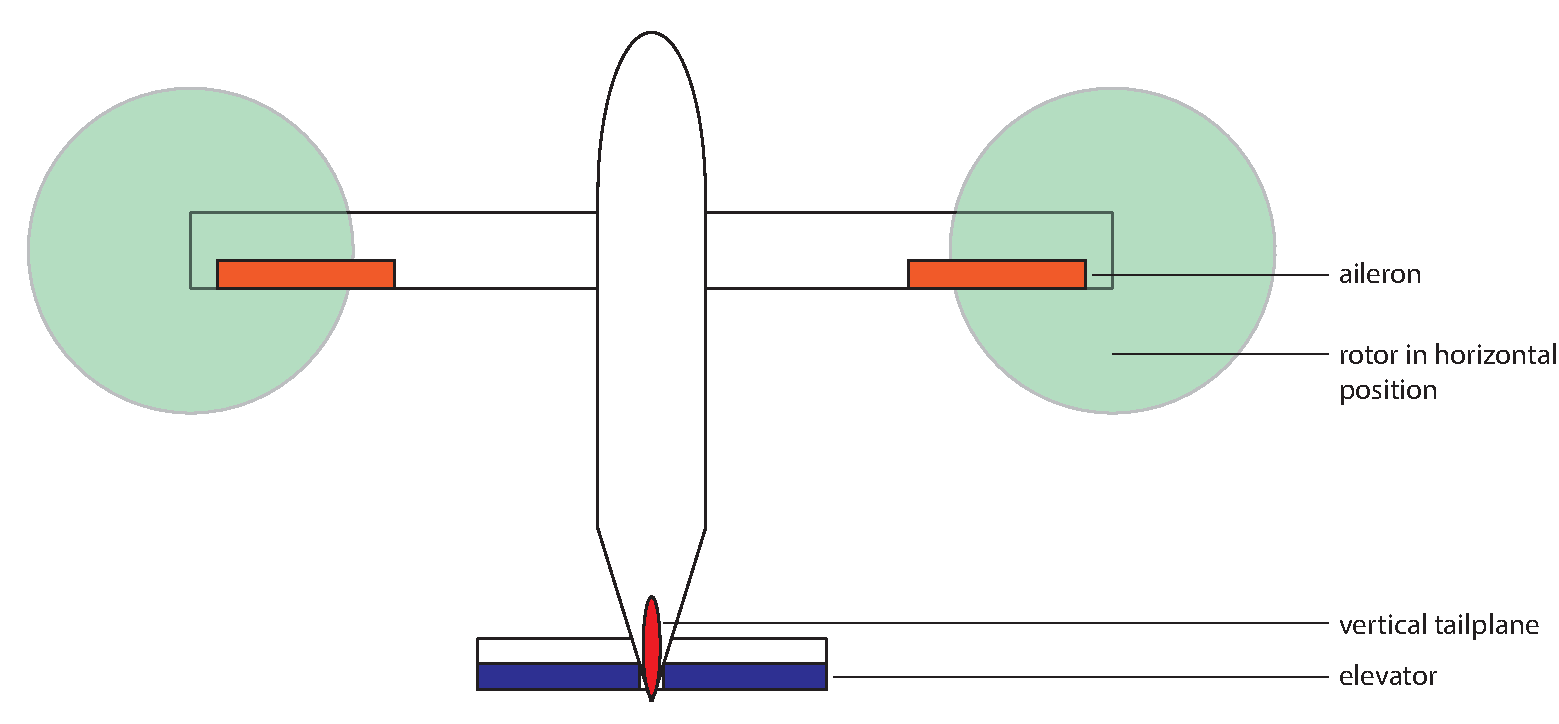
\includegraphics[height=6cm]{Stability/Figures/concept_4.pdf}
    \caption{Control Layout of The Tiltrotor}
    \label{fig:Ctr}
\end{figure}
\paragraph{Control}

The way of controlling the Tiltrotor concept was taken over from the V-22 'Osprey' transport craft and differs from both the co-axial and the three quadcopter-style designs. In \autoref{fig:Ctr} the controls of The Tiltrotor are laid out schematically.
In horizontal flight mode, The Tiltrotor relies on conventional aerodynamic control surfaces: a pair of ailerons on the main wing for roll control, elevators on the tail for pitch and a rudder for yaw. During vertical flight operations, those surfaces are ineffective, so the two engines mounted at the wing tips are used instead. Both of them can be tilted forward and backward independently and feature cyclic control swashplates\footnote{\url{http://janes.ihs.com/Janes/Display/1343214}, accessed 24-05-2017}. Pitch control is achieved by increasing the angle of attack of the forward or aft rotor blade with respect to the other one. This results in a lift asymmetry and therefore a control moment in longitudinal direction. Performing roll manoeuvres requires the collective pitch of one engines' rotor blades being different from the other one. Alternatively, the angular velocity of one engine could be varied while keeping the pitch equal, also creating a lift imbalance. Finally, yaw control in a 'helicopter mode' is done by tilting one engine forward and the other one backward. The tilted lift vectors create a net moment around the vertical axis.

The vehicle is controlled rather efficiently in horizontal flight because of the ideal layout of the control surfaces. In vertical flight phases of the mission, the attitude is controlled with the two wingtip mounted rotors. Because it will be virtually impossible to always let the centre of gravity coincide with the line connecting the two engines, a pitching moment needs to be generated by the engines to counteract the resulting thrust moment. Therefore, a continues cyclic input is usually needed in vertical flight to control the pitch angle of the UAV. 

\paragraph{Manoeuvrability}

The Tiltrotor is characterised by the two big engines located at the tips of its wing, which have a negative impact on its manoeuvrability. Especially roll performance is inferior to all other concepts due to the engine's large radius of gyration. While pitch inertia is nominal compared to the other concepts, yaw inertia also suffers from the engine placement. 

\paragraph{Stability}

In horizontal flight, The Tiltrotor is essentially a conventional configuration aircraft. The actual range of stable centre of gravity positions is dependent on a lot more detailed design considerations. However, conventional configurations are associated with relatively broad ranges of allowed centre of gravity positions. In contrast to The Tailsitter, this concept could conveniently incorporate a longer tail to increase this range even further. 

In vertical flight, The Tiltrotor is neutrally stable, as are all other concepts. The vehicle could be made laterally and longitudinally stable by implementation of a stabiliser bar of both rotors. 

% Lukas: Avy
\subsection{The Prandtl Box}
\begin{figure}[htb]
    \centering
    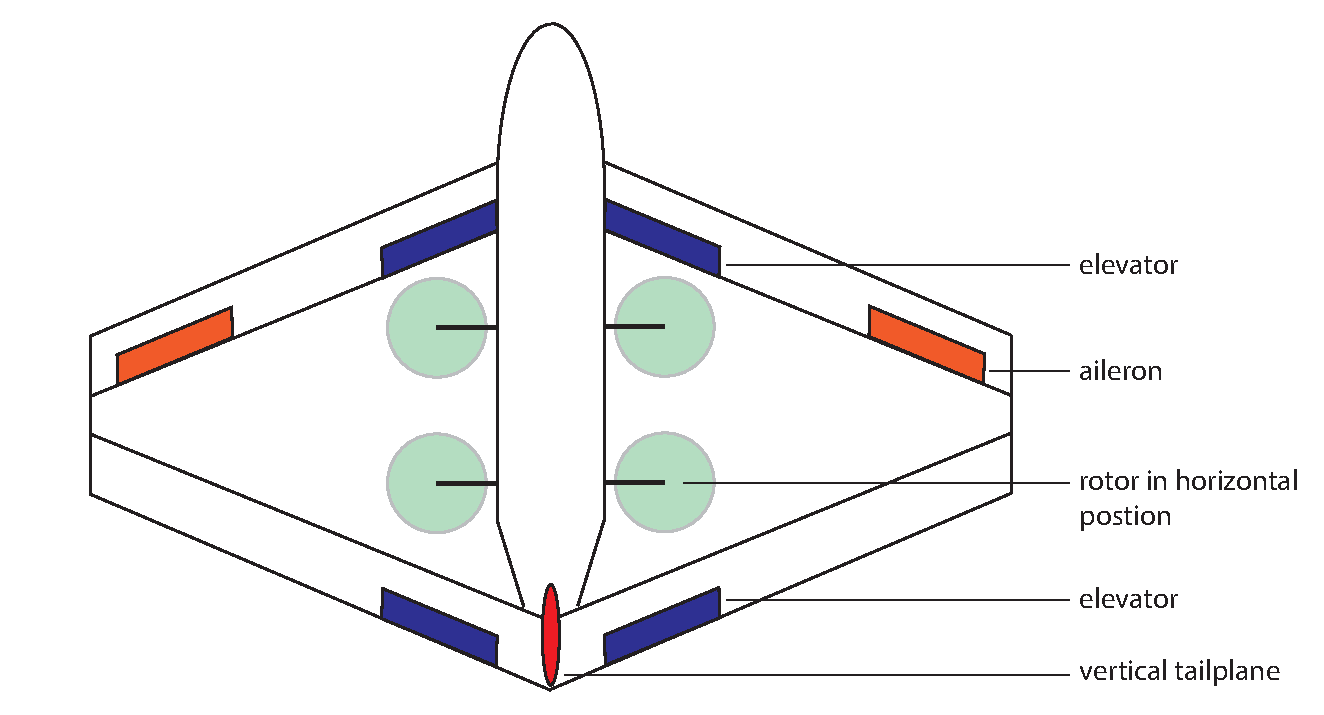
\includegraphics[height=6cm]{Stability/Figures/concept_3.pdf}
    \caption{Control Layout of The Prandtl Box}
    \label{fig:Cpb}
\end{figure}
\paragraph{Control}

The configuration of the control system of The Prandtl Box is shown in \autoref{fig:Cpb}.
From a control point of view, the Prandtl box is in many ways similar to the tandem wing. In this case, the wings are connected to each other and cannot move. Instead, the four engines are connected to the fuselage and can be tilted forward and upward. While this resembles the configuration of The Tiltrotor concept, no complex mechanisms are required for differential tilting or rotor pitch adjustments. In horizontal flight, a conventional setup was chosen for attitude control. The forward wing features two outboard ailerons for roll control, while the elevators are located on the back wing close to the body. The reason for this is the diamond shape of the wing layout, where the maximum moment arms for longitudinal control are achieved at the wing roots.
In vertical mode, the controls work similar to the ones on the tandem wing. Four pair-wise counter-rotating propellers with individual thrust settings provide pitch, roll and yaw control before being tilted for forward propulsion.

In conclusion, this concept has the same major drawback as the tandem wing configuration. The moment arms for the elevators are short in comparison to those in conventional configurations. Similar to the case of the tandem wing, this drawback is overcome by having elevators on both the front and aft wings to increase the amount of control surface area. The price to be paid for this solution is the increased trim drag caused by the greater control forces. The rudder also has a shorter moment arm, but it is used very little during flight. Therefore it's lower efficiency is acceptable. The aileron effectiveness for this concept is equivalent to that of the conventional designs since the aileron locations are as far outboard as possible while the wingspan is also similar. In vertical flight, the vehicle is essentially a quadcopter. The four rotors are positioned closer together in this design than in The Winged Quadcopter and The Tandem designs. This means that slightly more differential thrust is needed for the pitching and rolling moments. 

\paragraph{Manoeuvrability}

In terms of manoeuvrability, The Prandtl Box is comparable to The Tandem concept. The connection between the forward and backward wing introduces an extra component to the MOIs around the roll and yaw axis, however, the engines are mounted close to the body and therefore keep the MOI inertia nominal.

\paragraph{Stability}

Similar to The Tandem, The Pradtl Box has two approximately equally sized lifting surfaces. As with The Tandem, the centre of gravity should be slightly in front of the midpoint between the two wings. The aircraft can be stable about all axes. However, trimming becomes inefficient or even impossible for increasingly more forwards centre of gravity locations. 

In vertical flight, the quadcopter design renders it neutrally stable as no restoring forces are generated by any disturbance. The moment equilibriums about the vehicles axes are independent from attitude and are completely depending on the thrust of the individual propellers.

%Lukas: Jamaican cruiser
\subsection{The Winged Quadcopter}
\begin{figure}[htb]
    \centering
    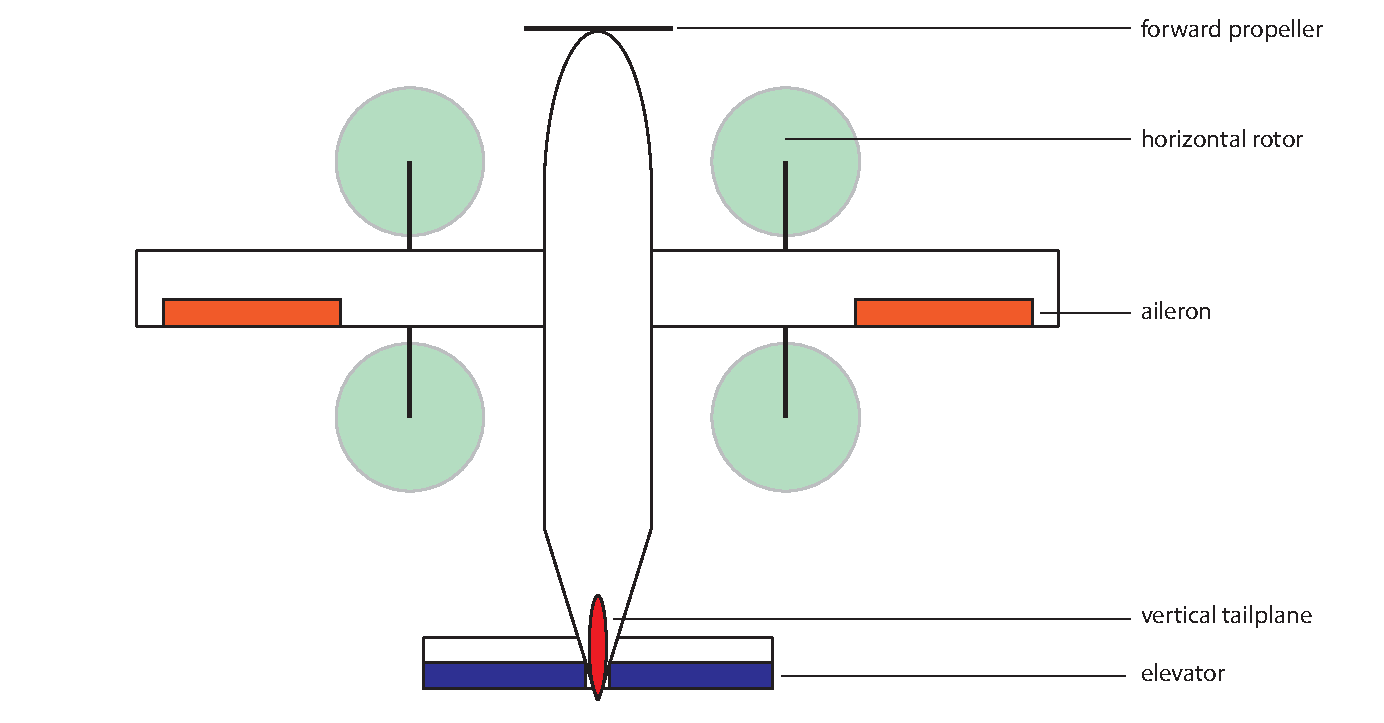
\includegraphics[height=6cm]{Stability/Figures/concept_5.pdf}
    \caption{Control Layout of The Winged Quadcopter}
    \label{fig:Cwq}
\end{figure}
\paragraph{Control}

Since this concept combines a conventional aircraft with a quadcopter, control is straightforward. The layout of the control system is depicted in \autoref{fig:Cwq}. In horizontal mode, it manoeuvres using elevators, ailerons and rudder, while in vertical mode differential thrust is applied in a fashion similar to the tandem and the Prandtl box concept. In horizontal flight, the conventional control layout results is effective and efficient control of the aircraft. In vertical flight, the quadcopter rotor configuration is also quite conventional. Only the increased distance between the rotors on the wing-mounted pylons is different. This reduces the amount of differential thrust needed for pitching and rolling control in a way analogous to The Tandem concept.

\paragraph{Manoeuvrability}

The Winged Quadcopter has a very low MOI around the roll axis, which comes close to the value The Tailsitter achieves with its central engine placement. The reason for this is the engine's placement relatively close to the fuselage, light wing and lack of wing-tip devices. Inertia values around the other two axis are the lowest of all five concepts, leading to the Winged Quadcopter being the most manoeuvrable one. 

\paragraph{Stability}

In horizontal flight, The Winged Quadcopter is no different from any other conventional configuration aircraft in terms of stability. The main wing provides most of the required lift during flight. A horizontal stabiliser at the tail provides stability for a considerable range of centre of gravity positions.
In vertical flight, The Winged Quadcopter is neutrally stable analogously to the other quadcopter designs discussed in this chapter.


    \chapter{Reliability Analysis}\label{ch:relianal}

In this chapter, separate aspects of the concepts that might influence the reliability of the designs are discussed. First, the performance of the different concepts on the analysed reliability aspects is summarised. Then propulsion system, control surfaces and wings are assessed. The energy source is briefly elaborated, but it is not taken along in the analysis since it does not differ per concept. The payload mounting systems are not included in the analysis either, since the different types of payload mounting systems do not pose any advantages or disadvantages in terms of reliability. 

The reliability of a subsystem is considered in two ways. The possibilities of failure are discussed, since they directly influence reliability. Also, a few values regarding the reliability of reference UAVs and other aircraft are presented when available.

\section{Trade-Off}
In this section, the final trade-off of the concepts is presented and then the grading system is explained. 

\subsection{Summary}
In this section, the reliability of the five concepts is compared in \autoref{tab:rel_ove}. The weights given to each reliability aspect are determined based on the sub-criteria. It is determined each sub-criteria is almost equally important. Only the control surfaces are slightly less important than the wing and propulsion reliability, therefore has been assigned with a slightly smaller weight. This is because it is still possible to continue flight and have certain control using the propulsion system when the control surfaces fail. The wing failure has a very large impact, since it is not even possible to make an emergency landing in that case. On the other hand, the probability of wing failure is very low in every case.

This assessment shows that The Tandem would perform the worst in terms of reliability, while The Winged Quadcopter is the most reliable design. 
\begin{table}[H]
    \centering
    \caption{Reliability sub trade-off}
    \label{tab:rel_ove}
    \begin{tabular}{r|>{\centering}p{3.5cm}:>{\centering}p{3cm}:>{\centering}p{3.5cm}|C}
    \textbf{Concept \rotatebox{90}{\hspace{0.5cm}Criterion}}            & 
    \rotatebox{90}{\textbf{Propulsion}}                                   &
    \rotatebox{90}{\textbf{\multicolumn{1}{p{2cm}}{\raggedright{Control surface}}}}     & 
    \rotatebox{90}{\textbf{Wings}}                                        &
    \rotatebox{90}{\textbf{Outcome}}
    \\ \midrule
    The Tailsitter      &  -    &  0  &   +    & 50\% 
    \\\hdashline
    The Tandem          &  + &  - &   -   & 42.5\% 
    \\\hdashline
    The Prandtl Box     &  0   & ++   &  ++ & 82.5\% 
    \\\hdashline
    The Tiltrotor       &  0    &  0    & + & 58.75 \% 
    \\\hdashline
    The Winged Quad.    &   0  &  ++   & +  & 73.75\% 
    \\ \midrule\midrule
    Weight          & 35    &   30  & 35   & 
    \end{tabular}
\end{table}

\subsection{Grading System}

In order to grade the reliability performance of the different concepts, the grading system of \autoref{tab:susweight} is used. 

\begin{table}[htb]
\centering
\caption{Definition of reliability grading system}
\label{tab:relweight}
    \begin{tabular}{ccc}
        \toprule
        \textbf{Rating}           & \textbf{Meaning}
        \\ \midrule
         ++            & Excellent reliability performance
        \\ \hdashline
        +   & Good reliability performance
        \\ \hdashline
         0          &  Average reliability performance
        \\ \hdashline
          -           & Bad reliability performance
        \\ \hdashline
         \texttt{-{}-}   & Unacceptable reliability performance
        \\ \bottomrule
    \end{tabular}
\end{table}

\section{Propulsion System}

In this section, the propulsion system of each design will be analysed and the reliability will be assessed. All configurations use electrical engines. Although engines have different performances using other power systems, it is assumed for the trade-off that each design uses the same battery and hence this discussion is not included in the following. 


Electrical engines and propellers are very reliable and can operate without failure for time period in order of 10 years.\footnote{\url{http://electroprop.com/100-reasons/}, Accessed 12-05-2017}$^,$\footnote{\url{http://www.mt-propeller.com/en/entw/products.htm}, Accessed 12-05-2017}

\paragraph{Double Propeller}
The Tailsitter design only uses one double propeller located at its nose for both horizontal and vertical propulsion. The fact that only one engine is used for propulsion makes the reliability of it critical. After engine failure, no more prolonged vertical flight is possible and the drone has no other option but to perform an emergency landing, either horizontally or using autorotation.\footnote{\url{http://www.copters.com/pilot/autorotation.html}, Accessed 22-05-2017} Engine failure will result in mission failure due to the emergency landing and on some minor damage created by the emergency landing.

\paragraph{Four Propellers}
The Tandem, the Prandtl Box and the Winged Quadcopter make use of four propellers for vertical flight as well as horizontal flight. In case of engine failure, three engines for horizontal control remain and a horizontal landing can still be performed. Although vertical landing is still possible using 3 engines on a quadcopter, the process is difficult and complex algorithms have to be used\footnote{\url{https://www.ethz.ch/en/news-and-events/eth-news/news/2013/12/new-algorithm-makes-quadrocopters-safer.html}, Accessed 11-05-2017}.
A difference between the Tandem and the other two designs is the rotating mechanism of the propulsion system. While the engines of the Tandem are fixed, the Prandtl Box and the Winged Quadcopter design use a rotating propulsion mechanism. Thus, the reliability also depends on the rotating mechanisms. Depending on whether the engines fail in horizontal or vertical mode, either a horizontal or a vertical landing has to be performed, which results in mission failure and a maintenance or replacement of the mechanisms.


\paragraph{Two Propellers}
The Tiltrotor uses the same rotational mechanism as the Prandtl Box. It only uses two instead of four engines for vertical, as well as horizontal flight. The reliability is based on the rotating mechanisms and engine failure. In case of engine failure, control during vertical flight is not possible anymore and a yawing moment is produced during horizontal and vertical flight. Two alternatives in case of engine failure are presented as following. One solution is to connect the second engine to the first one by a drive system in order to take control over both rotors. Another approach would be to perform a horizontal landing, in this case the torque created by the rotors has to be taken into account during the design of the rudder. The reliability of the rotating mechanisms can be compared to the one of the Winged Quadcopter design as on engine failure, enough control is still possible to perform a safe landing. 



\subsection{Power System}
Since each system is electric, a battery will probably be used as a main power source. Batteries are a reliable power source, but failure will have catastrophic consequences as they often are paired with fires.\footnote{\url{http://ijesat.org/Volumes/2012_Vol_02_Iss_05/IJESAT_2012_02_05_06.pdf}, Accessed 12-05-2017} Solar panels could be another potential energy source. These will most likely be used in combination with a battery, so the battery's reliability will remain critical. Solar panels are very reliable, with a life span of up to 25 years.\footnote{\url{http://greenzu.com/reliability-and-warranties}, Accessed 12-05-2017} 




\section{Control Surfaces}

In this section, the differences in reliability of the control system of each concept are discussed. This is dependent on the amount and type of control surfaces. In some concepts, failure of certain control systems can be compensated by the propulsion system or by the remaining control system. This has no impact on the reliability of the control system, but it does have an impact on the controllability. The reliability will be discussed per concept.


\paragraph{The Tailsitter}
The Tailsitter is mainly controlled by its control surfaces, making them a critical aspect of the design. It has ailerons that also act as elevators. It also has rudders. Both of these are generally very reliable \cite{reliability}. With the exception of cyclic and collective pitch control, the propulsion subsystem can not provide redundancy for the full range of flight conditions in case any of the control systems fail.

\paragraph{The Tandem}
The Tandem configuration has elevons near the tips of each wing. Besides that, it also has control surfaces at the rear wings' winglets to compensate for the lack of tail. These fulfil the function of a rudder. Since the tandem configuration has a rotor blade attached to each wing, these can provide some control in case of failure of any of the control surfaces. Control using propellers however might result in different angle of attack of the wings and produce even further instability. The reliability of the Tandems control surfaces is thus of critical importance. 

\paragraph{The Prandtl Box}
The Prandtl Box has ailerons on the front wing and elevators on both the front and back wing. It also makes use of a rudder in the tail. Since propulsive forces are applied by four engines at four different locations, redundancy is provided.

\paragraph{The Tiltrotor}
The Tiltrotor has ailerons in the wing and elevators on the horizontal stabiliser. It also has a rudder in the tail. This concept is very hard to control when hovering, since the centre of gravity location in fuselage-direction can differ. Since control in this flight mode is given by the rotors, these are critical to this design and should be very reliable.

\paragraph{The Winged Quadcopter}
The Winged Quadcopter makes use of both ailerons on the wings and elevators on the tail, as well as a rudder. The rotors mounted to the extensions on the wings can help control the UAV, making reliability of the control surfaces less important.





\section{Wings}
The wing layout of the concepts can be divided between conventional designs, wing layouts that are used frequently, and unconventional ones. The last category is not non-existent, but is not very common.


\paragraph{Conventional Designs}
The wings of the Tailsitter, the Tiltrotor and the Winged Quadcopter are all conventional designs. Their reliability can thus be compared to conventional aircraft. Here, statistical analysis shows that the reliability of conventional wings is above 99.99 \% for a 6 hours flight \cite{reliability}. This is, however, under the assumption that the wings are checked in constant intervals for cracks, damages, or any other signs of fatigue.

\paragraph{Unconventional Designs}
The Prandtl Box and the Tandem use unconventional designs. Their reliability will be discussed.


The general Prandtl wing configuration is reliable due to the structural advantage of the closed wing section. Since the concept was altered slightly, taking the engines out of the wing, this structural integrity is maintained. Therefore the Prandtl wing configuration is the most reliable one.

The most critical design in terms of wing reliability is the Tandem. This is due to the fact that not the engines themselves, but the wings can be rotated. Similar to the rotating mechanisms of engines in other designs, these mountings cause a reliability issue. This is because they have to bear the loads created by the wing and propulsion system. Many manufacturers have already observed that tilt-wing technology is riskier than tilt-rotor technology \cite{princeton}. Hence the reliability of the Tandem wings is classified lower than that of other designs. 


































\begin{comment}
COMENTED FROM HERE DON T CHECK, EXCEPT IF BORED...
\section{Preliminary Design 1: the Tailsitter}
%CONCEPT + critical points
The Tailsitter concept is a relatively simple design. It consists of a flying wing with two large rotor blades at its nose, and a vertical tail in two directions. It is controlled by control surfaces in the wing and two vertical sections, comparable to a tail. Since these are the only ways to fully control the UAV, their reliability is critical. The rotor blades are also a critical component as they are the only way to propel the UAV.



The presence of only one engine can cause safety issues. Failure of this component can be caused by for example overheating, over-current or vibrations.  


results in an absence of propulsion, making a vertical landing impossible. In this case, the UAV has no other option but to make a horizontal glide landing.

 


Main engine failure modes are due to overheating, over-current or vibrations. 
Vibrations can be prevented by regularly checking the engine alignment. Overheating and over-current can be avoided using good hardware and matching the power source to the engine type. These steps make it possible to decrease the probability of engine failure during flight. 


Stability might become an issue as only control surfaces are used to counteract torques created during hovering. The consequence of failure means that there is no more control over the aircraft 

and depending on the position the control surfaces are stuck

a crash can not be prevented.

The impact is thus considered high. 
??? this sentence should be rewritten -- really vague


Another concern for reliability is the centre of gravity range. As the design is based on a flying wing, during horizontal flight the centre of gravity is not allowed to change a lot in order to still provide static stability. The consequences of this failure are an unstable flight condition. 

This flight can be controlled depending on the intensity but should be avoided. 

The impact is thus considered medium. The probability of failure can be decreased using the right payload mounting procedures and equally distributing the payload inside the payload bay.

The final design can be categorised as reliable as the probability of most failure modes is low.  

\begin{table}[htb]
\centreing
\caption{Reliability analysis for the Tailsitter}
\label{tab:rel_tail}
\begin{tabularx}{\textwidth}{p{2cm}p{3cm}p{2cm}p{5cm}p{2cm}}
\toprule
    \textbf{Part} & \textbf{Failure Cause} & \textbf{Probability of failure} & \textbf{Consequences} & \textbf{Impact} \\\midrule
    Engine & Overheating  & Low & No vertical flight / \\ 
    & Over-current & Low & Horizontal emergency landing & Medium \\
    & Vibrations & Low &necessary\\\midrule
    Control surfaces & Mechanical & Low & No more flight control  & High \\\midrule
     Payload & Change in c.g. & Low & Unstable flight & Medium \\\bottomrule
\end{tabularx}
\end{table}

\section{Preliminary Design 2: the Tandem} 

The tandem wing design is a relatively complex design. It uses rotatable wings for control in vertical flight. These are the most critical part of the design and should be reliable. In horizontal flight four engines produces the necessary thrust and different control surfaces are used. Although these parts are important for horizontal flight, failure of an engine causes a lower impact. 


Considering reliable properties, the fuselage can be considered as a simple structure to hold the payload. Also as the wings are rigid systems mounted at the front and back of the fuselage, centre of gravity shifts do not cause a big concern. 


The first reliability concern comes from the landing gear. As the plane will land at landing wedges on each end of the wings, a too high landing speed might damage the wings. The consequences are a damaged landing wedge that needs to  be repaired. This can be prevented using controlled landing procedures.


Furthermore, the wings are mounted on the fuselage using a rotation mechanism. All forces carried by the wing are transferred to the fuselage through these mountings, meaning they have to be designed for high stresses in order to avoid failure. The biggest reliability concern of these connections comes however from the rotating mechanisms themselves. In addition to carrying the loads, they should be able to rotate the wings from vertical to horizontal mode. To reduce the probability of failure, regular inspection of the wing mountings should be carried out. 


In case of an engine failure, the same causes as for the previous design apply. However there are still 3 other engines available which can be used for horizontal flight. Vertical flight will not be possible anymore however and mission failure could be the consequence. 

In case of control surface failure, the rotation of the wings can still be used to control the aircraft, hence the impact is reduces to medium compared to the tailsitter design. 


\begin{table}[htb]
\centering
\caption{Reliability analysis for the Tandem}
\label{tab:rel_tail}
\begin{tabularx}{\textwidth}{p{2cm}p{3cm}p{2cm}p{5cm}p{2cm}}
\toprule
    \textbf{Part} & \textbf{Failure Cause} & \textbf{Probability of failure} & \textbf{Consequences} & \textbf{Impact} \\\midrule
    Landing wedges & Impact Landing & Medium & Required maintenance & Low\\\midrule
    Engine & Overheating  & Low   \\ 
    & Over-current & Low & No vertical flight & Low \\
    & Vibrations & Low &\\\midrule
    Wings &Structural & Low & Loss of wing & High \\
    & Rotational & Medium & Loss of vertical control & Medium\\\midrule
    Control surfaces & Mechanical & Low & Less flight control & Medium \\\bottomrule
\end{tabularx}
\end{table}



\section{Preliminary Design 3: the Prandtl Box}

In this design, the wing and tail are connected to the fuselage using a closed-Prandtl configuration. This leads to a rigid structure where everything is interconnected. 

The design has some structural reliability issues as the engines are mounted inside and in between the wings. This will create stress distribution which have to be carried by the interconnecting structure as well as by the wings. The impact of this failure is high due to the critical role of the wings. The design of a stiff and safe structure is of major importance to avoid failure. 

Then the engines can be rotated for VTOL. This creates moving mechanisms which are susceptible to failure. If one of the actuators fails, the corresponding engine might become unavailable depending on its final position. Horizontal flight is still possible with the remaining engines however vertical control can not be used anymore. The probability  

For the Prandtl Box, the structural reliability issue is solved using an adequate design for the loads and regular inspection and maintenance. The reliability in engine failure can be kept small using adequate engines and the failure of mechanisms can be lowered using appropriate mountings. Due to these engine reliability issues, the Prandtl Box is categorised as sufficiently reliable. 

\begin{table}[htb]
\centering
\caption{Reliability analysis for the Tandem}
\label{tab:rel_tail}
\begin{tabularx}{\textwidth}{p{2cm}p{3cm}p{2cm}p{5cm}p{2cm}}
\toprule
    \textbf{Part} & \textbf{Failure Cause} & \textbf{Probability of failure} & \textbf{Consequences} & \textbf{Impact} \\\midrule
    Engine & Overheating  & Low & No vertical flight / \\ 
    & Over-current & Low & Horizontal emergency landing & Low \\
    & Vibrations & Low &necessary\\
    & Rotational Mechanism & Low & Loss of vertical control & Medium \\\midrule
    Wings & Structural failure & Low & Crash & High \\\midrule
    Control surfaces & Mechanical & Low & Less flight control & Medium \\\bottomrule
\end{tabularx}
\end{table}





\section{Preliminary Design 4: the Tilt-rotor}

This design is based on a conventional aircraft configuration which makes it reliable in terms of horizontal flight. However, only two engines are used. In case of engine failure, gears could be designed to link both engines. In this way, the remaining engine could also drive the second engine in order to still be able to perform a safe landing. This will however increase the complexity of the design. Furthermore, the engines themselves rotate in order to produce either horizontal or vertical thrust. In case of rotation failure, the unmanned aerial vehicle is not able to produce either horizontal or vertical thrust depending on the engine direction during failure. The reliability issue of this mechanisms is also of moderate order.
Control during vertical take-off and landing is another reliability issue. The rotors have to rotated constantly to make the line of action of the thrust coincide with the centre of gravity in order to avoid instabilities. This can be achieved using a reliable algorithm. 

The only issue not solved for is the case for a failure of the actuators for rotating the engines. Using advanced mechanisms the probability of failure can be reduced, however not removed. For this reason, the Tilt-rotor is sufficiently reliable.


\section{Preliminary Design 5: the Winged Quadcopter}

The last design is a really simple one. Using a conventional and thus reliable aircraft configuration for horizontal flight. For vertical flight, 4 rotors are used mounted at the wings. The mountings have to carry the load of the fans and the thrust required for vertical flight. In order to reduce probability of failure, they should be designed for stiffness. The only unreliable part are the rotational mechanisms of the rotors. They have to be rotated several times during each mission and hence failure of the rotation results in failure of the mission.   
A small reliability issue can be found in the centre of gravity position. As the payload is mounted in the fuselage, care should be taken that the payload is distributed in a way that the centre of gravity does not shift to much forward in order to provide static stability.

As with the previous design using rotating engines, the reliability of the system primarily depends on the reliability of these rotating mechanisms. For this reason, the design is categorised as sufficiently reliable. 
 
\end{comment}
    \chapter{Production Cost Analysis}
\label{ch:costanal}
%not prodcostanal, name has been changed later on, leave costanal as it has been used everywhere already. Next time make it with underscores as was the convention

The production cost of an aircraft comes from multiple aspects, to combine the results of these aspects a trade-off has been made presented in \autoref{sec:subtradcost}. The cost has been split up into five different categories: manufacturing cost, material cost, mechanism cost, power \& propulsion cost, and influence of weight on cost. The reason behind this division, the assigned weights and a brief explanation on the different categories will be provided in \autoref{sec:costcrit}. The production cost and layout of a conventional plane, scaled to the average weight of the concepts, are taken as a nominal value. The production cost of the nominal value will be estimated in \autoref{sec:nomval}. To do the trade-off with respect to cost, the concepts will be compared to this nominal value in \autoref{sec:conanal}. In this way, it is possible to assess if the costs of the concepts will be higher or lower than the nominal production cost.   

\section{Cost Trade-off}
\label{sec:subtradcost}
In this section, the cost trade-off will be presented and the results will be discussed. The grading system will also be described.

\subsection{Summary}
The trade-off table can be seen in \autoref{tab:costsubtradja}. The trade-off will provide the reader with an overview that visualises the result of all categories of costs and its corresponding weights.


\begin{table}[H]
    \centering
    \caption{Cost sub trade-off}
    \label{tab:costsubtradja} %please use your own label when you copy it!
    \begin{tabular}{r|>{\centering}p{2.5cm}:>{\centering}p{1.5cm}:>{\centering}p{1cm}:>{\centering}p{3cm}:>{\centering}p{2cm}|c}
    \textbf{Concept \rotatebox{90}{\hspace{0.5cm}Criterion}}    & 
    \rotatebox{90}{\textbf{Manufacturing}}                      &
    \rotatebox{90}{\textbf{Material}}                           & 
    \rotatebox{90}{\textbf{Mechanism}}                          & 
    \rotatebox{90}{\textbf{Power \& Prop}}                      & 
    \rotatebox{90}{\textbf{Mass}}                             &
    \rotatebox{90}{\textbf{Outcome}} 
    \\ \midrule
    Tailsitter      & + +   & + +   & - -   & - -   & 0     & 50\% 
    \\\hdashline
    Tandem          & -     & -     & -     & +     & -   & 36.25\% 
    \\\hdashline
    Prandtl Box     & - -   & - -   & +     & +     & + +   & 50\% 
    \\\hdashline
    Tiltrotor       & 0     & - -   & - -   & -     & - -     & 20\% 
    \\\hdashline
    Winged Quad.    & 0     & 0     & 0     & 0     & +   & 55\% 
    \\ \midrule\midrule
    Weight          & 25    & 15    & 10    & 30    & 20    &  
    \end{tabular}
\end{table}

With an outcome of 55\%, The Winged Quadcopter has the highest score of all concepts with respect to costs. The Winged Quadcopter scores no minuses on the general criteria since the configuration of this concept is very similar to the nominal aircraft, one plus is scored on the influence of weight. There are some differences in the configuration of The Winged Quadcopter, e.g., the extra beams to hold the propellers but these differences are negligible with respect to cost. Its low weight makes the concept have a high resulting score. 
The second best concepts, with only 5\% less than the first one, are The Tailsitter and The Prandtl Box. The Tailsitter has low costs for manufacturing and material since it is a flying wing. However, using a single, engine with counter-rotating propellers for propulsion is expensive and requires expensive mechanisms for control. The Prandtl Box also scores high while having a complex wing which is very difficult to manufacture and a fuselage requiring substantial structural strength; its weight gave it its high score.

The next concepts have a score which differs a lot from the first three ones. This means that these concepts are clearly more expensive than the previous three. The Tandem has minuses for everything except the propulsion sub-criterion. It scores good on propulsion because of its four engines. The UAV with the lowest score is The Tiltrotor scoring minuses on every sub-criterion except for manufacturing costs. 

In short, The Tailsitter, The Prandtl Box and The Winged Quadcopter are the obvious winners of the cost trade-off. The other concepts have clear disadvantages with respect to cost. 

\subsection{Grading System}

The trade-off grading has been done by assigning pluses, minuses and zeroes to every concept on multiple cost criteria. In this way, the table gives a clear overview of what the concepts score relatively to each other and to the nominal value for each sub-criterion. \autoref{tab:costweight} shows the explanation behind the grading system used. 

\begin{table}[H]
\centering
\caption{Definition of cost grading system}
\label{tab:costweight}
    \begin{tabular}{rl}
        \toprule
        \textbf{Rating}           & \textbf{Meaning}
        \\ \midrule
         + +            & Excels          
        \\ \hdashline
        +               & Better
        \\ \hdashline
         0          & Average 
        \\ \hdashline
          -           & Worse 
        \\ \hdashline
         - -    & Bad  %how about this? Poor is also an option, or erroneous; uh uh, and unacceptable is unacceptable in this context, don't delete the comment x_x
        \\ \bottomrule
    \end{tabular}
\end{table}

To calculate the outcome of the trade-off, each criteria score will be multiplied with the corresponding weight, with each '+' being equal to 1 and each '-' being equal to -1. The highest possible score would be 200 while the lowest possible score would be -200. For ease, this scoring should be scaled from 0 to 100. In order to do this, the outcome shall be divided by four (to reduce the range from [-200,200] to [-50,50]). Finally, 50 will be added to this number to bring the range to [0,100].

\section{Cost Criteria}
\label{sec:costcrit}
This section will describe and discuss the different cost criteria used in the trade-off, in \Cref{sec:mancost,sec:matcost,sec:mechcost,sec:powercost,sec:weiginflcost}. The reasoning behind the assigned weights of the criteria will be explained in \autoref{subsec:critweightcost}. 

\subsection{Manufacturing Costs} 
\label{sec:mancost}
The manufacturing costs depend greatly on the complexity of the aircraft. The production of a more complex aircraft requires more man-hours, a bigger facility, more material, better tools or simply more time to be produced; which all cost money. To know what the share of each aspect is in the total manufacturing cost, a brief analysis has been made. \autoref{tab:manucosts} shows the percentage of costs for labour, materials and other costs of the manufacturing process\footnote{https://dspace.mit.edu/bitstream/handle/1721.1/16871/51679351-MIT.pdf?sequence=2, Accessed 11-05-2017}.


This table shows that most of the manufacturing cost, around 41\%, goes into labour. The 'other' costs take up around 26\% of the manufacturing cost and 33\% goes to the material cost. In this trade-off, the manufacturing cost includes the labour and other cost. The material cost will be a separate criterion which will have a weight that is approximately half the weight of the manufacturing cost. 

\begin{table}[H]
    \centering
    \caption{Percentages of manufacturing costs}
    \begin{tabular}{cccc}
    \toprule
         & Labour & Materials & Other \\ \midrule
    \% of costs     & 41 & 33 & 26 \\
    \bottomrule
    \end{tabular}
    \label{tab:manucosts}
\end{table}

The first aspect of the manufacturing cost is the 'other costs' which are costs for quality assurance, and the required tools and machines. These will be seen as facility related costs. The facility needed depends on a few factors: machines, tools, complexity of assembly, and complexity of the concept. The machines and tools needed differ for each concept: one might need a machine which can bend sheets to make wings with double curvature while other concepts might need big and complex tools such as moulds for laminating the wings. The complexity of assembly also plays a role: a concept might require assembly of different parts of the wings, while other concepts are able to build the wing in one piece. When the complexity of the assembly increases, the required man-hours  and amount of assembly lines also increase.

The second aspect of the manufacturing costs is the amount of man-hours needed to manufacture the UAV. Time is money, hence the longer the process, the more it will cost. To assess the time needed to manufacture the UAV, the concepts will be analysed on how complex they are.

\subsection{Material Costs} 
\label{sec:matcost}

A higher amount of material or using a more expensive material means it will have a higher cost. Even though material costs are actually a part of manufacturing costs, the decision has been made to separate these two aspects because the material costs may have a great influence on the price of the UAV. If these two aspects were put together, a UAV with a low material cost but complex shape, hence high manufacturing cost, will eventually lead to a medium value for the total cost, not showing which aspect is expensive or not. In this case, using two separate aspects is more insightful. 

To assess whether or not the concept will have high material costs, rough estimates need to be made of how big the concept will be and how it will handle stresses in comparison to the nominal value. If, for example, a UAV has heavy engines on the tip of a wing, strong and heavy wingboxes will be necessary to support the structure. Hence, the material cost will be larger than for a conventional aircraft. Another example is that a concept might have a lot of surface area, increasing the material needed to build the concept which will increase the cost.

\subsection{Mechanism Costs}
\label{sec:mechcost}

When dealing with Hybrid UAVs, the designs may have a lot of movable parts. For this reason the concepts will be analysed for the extent to which they rely on complex, hence expensive mechanisms: will they have rotatable engines, movable wings or other moving parts. To move these parts, actuators will be needed and integrated into the design. These actuators will also have influences on the manufacturing cost and power cost, but those influences will be assessed in the respective criteria. In this criterion, purely the costs of the mechanism will be analysed.

Not only the movable parts unique to a specific Hybrid UAV will be analysed for these costs, but also the control surfaces. Possibly, one concept will have less control surfaces than a conventional aircraft, hence having less mechanism costs, or have a complicated swash plate in order to control the UAV.

\subsection{Propulsion \& Power Costs} 
\label{sec:powercost}

The Propulsion \& Power cost is a big cost with respect to the total cost of the UAV. Also, the propulsion cost may differ significantly between the concepts depending on the number of engines. Since propulsion and the power needed for propulsion are closely related to each other, these two criteria are grouped together. 

\subsection*{Propulsion Costs}
\label{sec:propcost}
Within propulsion costs there are two things that could be taken into account: the propeller costs and the engine costs. It can be assumed that the propeller cost doubles when the amount of propellers double, but the cost for the propellers are negligible in comparison with the engines costs.To find the cost of the engines, some literature study must be made to find the price of certain engines, the ratio of cost over power, the ratio of cost over torque and how the price relates to the number of engines used. 

The case of vertical climb is analysed since this is the flight phase where most power is needed.
The first step taken in order to estimate the costs of the propulsion system was to find an equation for the power required during vertical climb. Use is made of \autoref{eq:goodpow}\footnote{\url{http://s6.aeromech.usyd.edu.au/aerodynamics/index.php/sample-page/aircraft-performance/hoverclimbdescent-analysis/}, Accessed 18-05-2017} 

%which is derived in Appendix \autoref{chap:preq}.

\begin{equation}\label{eq:goodpow}
    P_{req} = T \cdot \left( \frac{V_{c}}{2} + \sqrt{ \left( \frac{V_{c}}{2} \right) ^2 + \frac{T}{2 \rho A}} \right)
\end{equation}

The equation shows that the power required depends on the climbing speed, the required thrust, the air density and the surface area of the propellers.  One can see that the thrust needed in order to climb vertically at a certain acceleration is equal for all concepts since it is assumed that the mass is equal for all concepts. It can also be assumed that the total propeller area is the same for every concept. Furthermore, the density at 2000m is taken in this equation. From this it can be concluded that the power required to climb at a certain acceleration and velocity will be the same for all concepts with any number of engines.

Two other parameters related to power play an important role when looking at engines: the torque and Rounds Per Minute (RPM). These two values make the difference between a cheap engine and an expensive engine. The cost of the engine will be higher for engines with higher torque and with lower RPM, since power is equal to torque times RPM.  

The airflow  over the propeller cannot be supersonic because the vibrations coming from the shock waves could destroy the propeller. Therefore, the tip velocity of the propeller will determine the maximum allowable RPM for a given propeller. The maximum RPM follows from \autoref{eq:tipspeed}.

\begin{equation}\label{eq:tipspeed}
\begin{aligned}
    %\text{Knowing the radius, r,}&\text{ from the required propeller area:}\\
    V_{max} =& 0.9 \cdot a \\
    \omega_{max} =& \frac{V_{max}}{2 \pi r} \Big[\frac{rad}{s}\Big] \\
    RPM =& \frac{V_{max}}{2 \pi r} \cdot \frac{60}{2 \pi} \Big[\frac{rev}{min} \Big]
\end{aligned}
\end{equation}

The maximum tip velocity has been taken as Mach 0.9 in order to prevent local shock waves to occur too. Knowing the maximum RPM, it is possible to calculate the minimum torque in order to generate the required power:

\begin{equation}\label{eq:powtor}
    \tau = \frac{P}{\omega}
\end{equation}

Knowing the maximum possible RPM and minimum torque to get the required power, it is possible to look at the costs of the propulsion system for engines with different torques and power settings. Statistical data was collected in order to find the relation between power and cost, and torque and cost in \autoref{fig:costvspow} and in \autoref{fig:costvstor} respectively. Both graphs show that the relation with cost is linear for power and for torque. It is assumed that the trend line for cost vs power and torque intersects at the origin.

%\begin{comment}
\begin{figure}[htb]
    \centering
    \begin{subfigure}[b]{0.45\textwidth}
        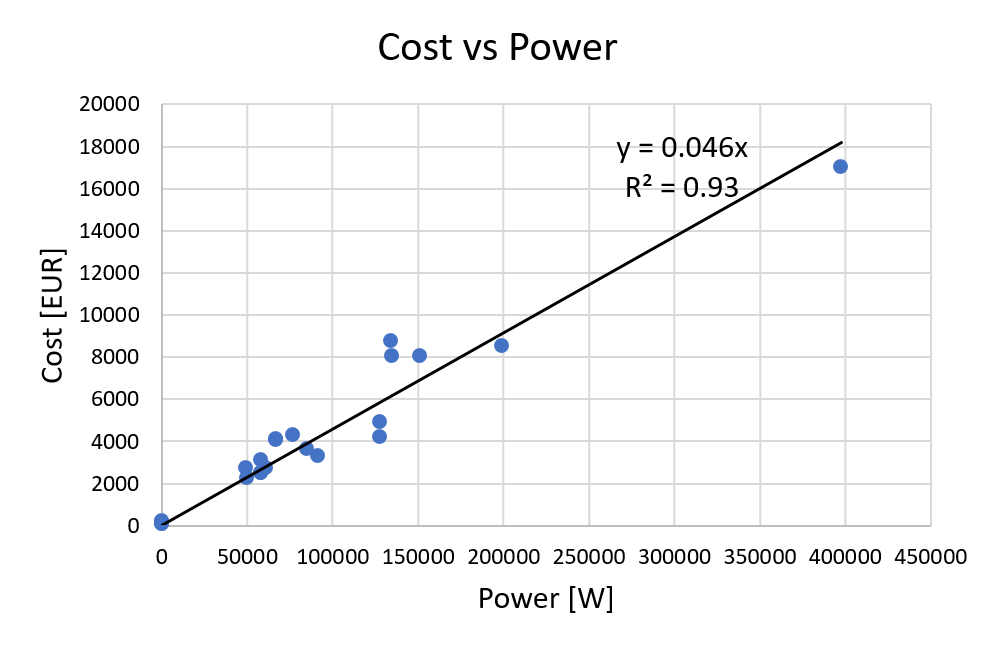
\includegraphics[width=\textwidth]{CostAnalysis/Figures/costvspower.PNG}
        \caption{Cost versus power relation}
        \label{fig:costvspow}
    \end{subfigure}
    \begin{subfigure}[b]{0.45\textwidth}
        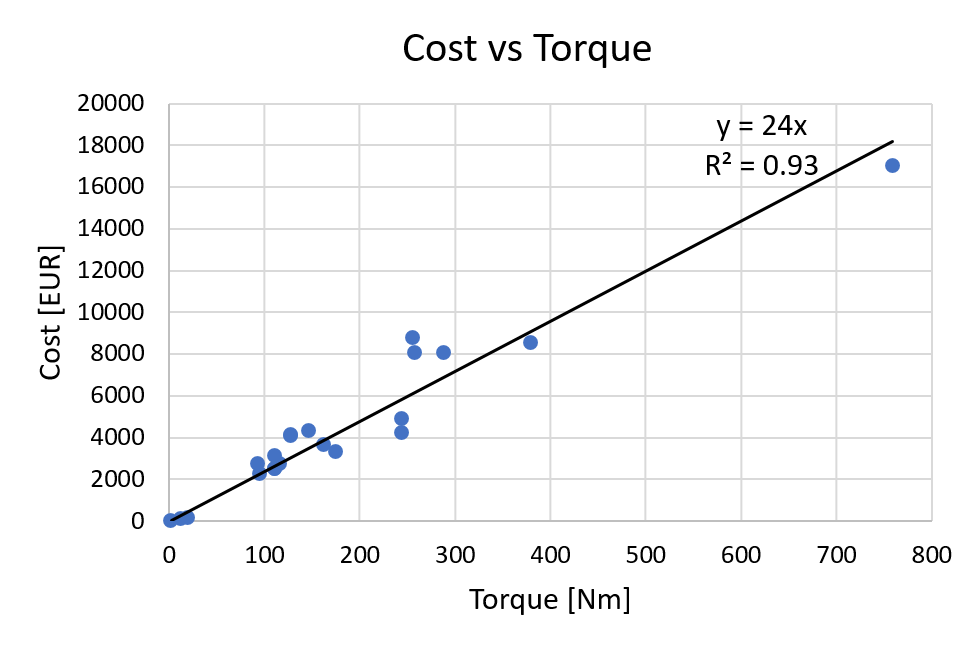
\includegraphics[width=\textwidth]{CostAnalysis/Figures/costvstorque.PNG}
        \caption{Cost versus torque relation}
        \label{fig:costvstor}
    \end{subfigure}
    \caption{Cost trendlines for torque and power}
    \label{fig:costtrendlines}
\end{figure}
%\end{comment}


When considering that the power required to climb is the same for each concept, one may think that the cost will be equal too. That is not the case since the tip velocity limits the RPM hence a minimum torque is required. In some cases, an engine with this limiting amount of torque may be more expensive than the value that can be seen for the power required. \autoref{fig:clearance} shows the total cost of engines depending on the propeller's area for different numbers of engines. An acceleration of 4 $\frac{m}{s^2}$, a $V_c = 4$ $\frac{m}{s}$ and a mass of 52 kg is taken. The cost is taken versus the propeller area because it is the same for different numbers of engines and it also resembles the radius of a specific number of engines which limits the maximum RPM. When having one propeller, a larger radius is needed in order to have the same total propeller area as a two/four propeller UAVs. This means the maximum allowable RPM will be lower, requiring a larger torque to achieve the amount of power. The power cost constraint will stay the same for different amounts of propellers since it only depends on the area which is the same for all number of engines.


\begin{figure}[htb]
    \centering
    \begin{subfigure}[b]{0.53\textwidth}
        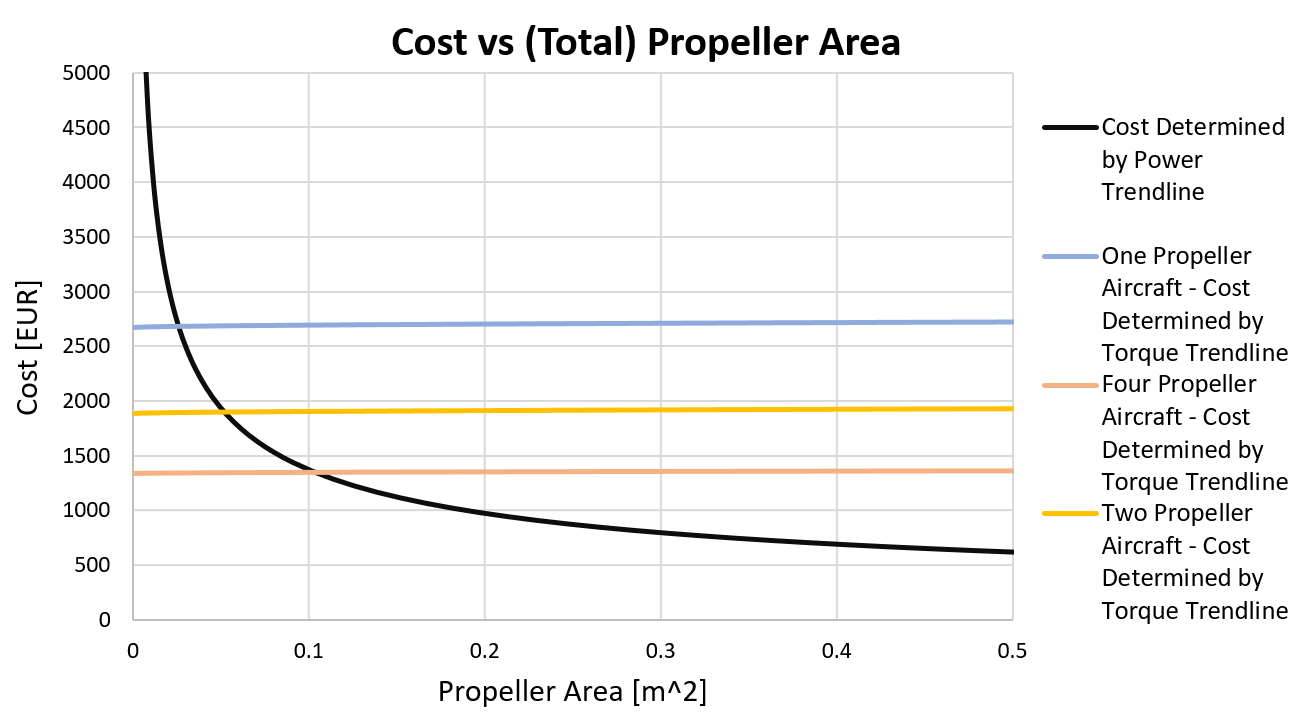
\includegraphics[width=\textwidth]{CostAnalysis/Figures/costvsarea2.PNG}
        \caption{cost vs propeller area}
        \label{fig:clearance}
    \end{subfigure}
    \begin{subfigure}[b]{0.45\textwidth}
        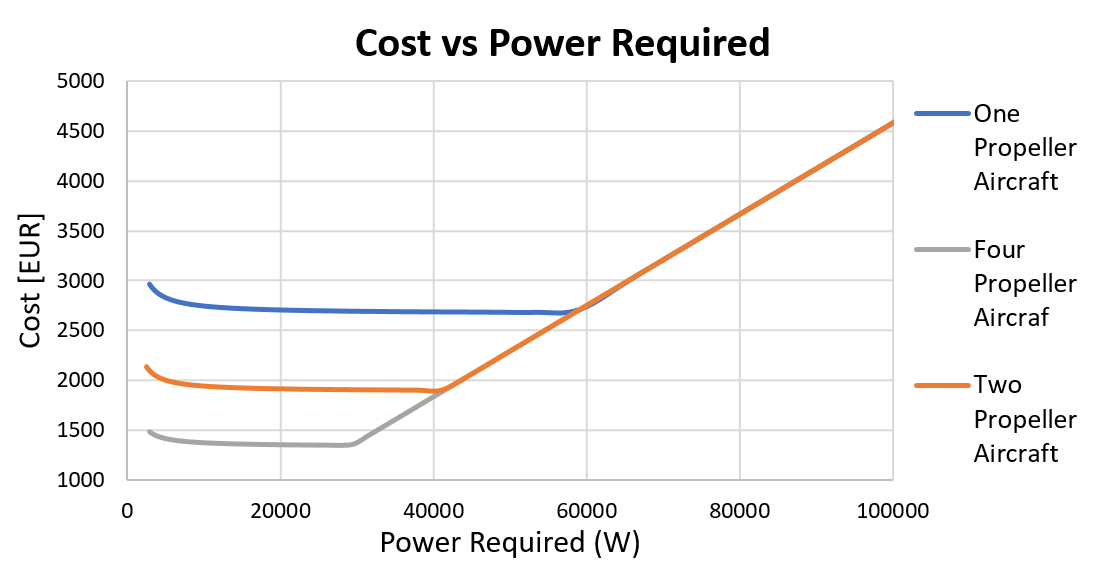
\includegraphics[width=\textwidth]{CostAnalysis/Figures/costvspower3.PNG}
        \caption{Cost versus power}
        \label{fig:costvspower}
    \end{subfigure}
    \caption{Cost graphs for one two and four engines}
\end{figure}

What can be seen in \autoref{fig:clearance} is that the cost is first determined by a power constraint and when the propeller area becomes larger it is determined by the minimum torque required. The point where the lines cross, is the point where the cost determined by the torque starts to take over. While the power required decreases vastly for an increase in propeller area, the torque required is increasing ever so slightly. \autoref{fig:costvspower} shows the highest cost for each UAV with respect to the power required.


It is interesting to notice that for a high power required, which corresponds to a small propeller area, the costs are the same for different numbers of engines. The point where the torque determined cost meets the power determined cost is the point with minimal cost. When the power required gets even smaller, the cost starts to increase heavily. This is due to the required minimum torque which is increasing to keep the required power while the angular velocity is decreasing due to the supersonic constraints. 

Going back to the effect of having multiple engines in comparison to one, the results show that it is more cost efficient to have multiple engines. A four time increase in engines may decrease the cost by half when the torque limits the cost (left side of the graph). When looking at the side where power limits the cost, having multiple engines or only one engine doesn't change the cost of the engine. So eventually, it all leads to the size of the propellers which determines the area, which determines the required power. Having them too small will mean the power required is very high, which means the UAV will have expensive engines due to the power determined cost. Having big propellers will mean that the torque needs to be big because of the low angular velocity required to prevent local sonic flow conditions, causing the cost to increase as well. 

When assuming that the power required is kept on the left side of the graph, then a four times increase in number of engines leads to a two times decrease in cost. If the total power remains the same for four engines, the power per engine will be one fourth. Also, having four engines instead of one means that the required propeller radius will be halved for each of the propellers. Looking at \autoref{eq:prooftor}, it is shown that the angular velocity will be doubled for a halved radius. The subscripts 'four' and 'one' clarify how many engines the UAV has.

\begin{equation}\label{eq:prooftor}
\begin{aligned}
    \omega_{four} = \frac{V}{2 \pi r_{one}} = \frac{V}{\pi r_{four}} = 2 \omega_{one}
\end{aligned}
\end{equation}

Using this relation to calculate the required torque yields:

\begin{equation}\label{eq:prooftor2}
    \tau_{tot_{four}} = \frac{P}{\omega_{four}} = \frac{P}{2\omega_{one}} = \frac{1}{2} \frac{P}{\omega_{one}} = \frac{1}{2}\tau_{tot_{one}}
\end{equation}

The total torque on a four-engine aircraft will be halved. Seeming that the torque determined cost is linear, the cost will also be halved. The relationship between number of engines and torque determined cost is: an N times increase in engines is $\sqrt{N}$ decrease in cost.


\subsection*{Power Costs}

The more power needed the more energy storage will be required. No definite choice has been made whether the Hybrid UAV will be using electric propulsion or not, but even when the propulsion would be combustion based, batteries will be needed. These will be needed to start the aircraft, rotate certain parts and move the mechanisms. Since batteries have a high price per kWh (around 175 euro / kWh)\footnote{https://electrek.co/2017/01/30/electric-vehicle-battery-cost-dropped-80-6-years-227kwh-tesla-190kwh/, Accessed 15-05-2017} the amount of energy needed will play a big role in the costs trade-off. 

To make a rough estimate of the cost of the power subsystem, a look needs to be taken in the subsystems that are using that power: the propulsion system (especially if electric), the mechanisms, the instruments and the Central Processing Unit (CPU). The propulsion system takes up the most power. To distinguish battery cost for the different concepts, the concepts will be analysed on how efficient they can fly. Hence, using less energy and a smaller amount of extra subsystems that need power. For example, when using a lot of mechanisms, such as rotating wings, more power is needed and the cost will be higher. Also, fans are more efficient than propellers when flying under 160 km/hr. Therefore, fans use less power making the power subsystem cheaper\footnote{http://www.esotec.org/hbird/HTML/DuctMyths\_F.html, Accessed 22-05-2017}.


\subsection{Weight Influence on Costs}
\label{sec:weiginflcost}

The weight of the concepts will greatly influence the production cost because weight is indirectly involved with all aspects of cost. To analyse the effects of cost, a look will be taken into each sub-criterion to find out how weight affects it. For the analysis of the other sub-criteria, the weight of the concepts will be considered as equal. In this way, the differences between the concepts on one sub-criterion can be found without interference of the other factors.

\paragraph{Manufacturing Costs} When the weight of a concept increases, the manufacturing cost goes up too. Not only will the facility needed to build the aircraft increase in size, but all tooling, machines and further equipment (e.g. moulds) will need to be bigger and thus cost more.

\paragraph{Material Costs} When the concept weighs more, there will be stronger forces on the aircraft: more lift, more drag, more thrust, stronger bending moments, and so on. To withstand these forces the structure needs to be stronger, requiring more structural components, thicker material or stronger materials. Another increase in cost comes from the fact that there will be more lift needed to lift the aircraft in horizontal flight, which comes from larger surfaces (e.g. wings and tail planes). These will increase the surface area of the aircraft and more material will be needed.

\paragraph{Mechanism Costs} The only change in costs at the mechanisms is that bigger and more complex mechanisms may be needed to hold the weight of the aircraft. This extra cost is assumed to be not as much as the other increases.

\paragraph{Power \& Propulsion Costs} This group is most affected by weight. The extra weight will influence a lot of the aircraft, which all influences the amount of power  needed. It first starts with the thrust needed to fly the aircraft vertically. An increase in weight means more thrust is needed which in turn means that the engines need to provide more power. A bigger, heavier and more expensive engine will be the result. Some bigger propellers may also be needed, but this cost is negligible with respect to the engine. Due to the heavier engines, more power will be needed to power them, so bigger batteries are necessary. More power will also be needed to move certain parts with the same speed(e.g. rotating wings with The Tandem) due to the parts being heavier and having a bigger moment of inertia. Though this extra power required is negligible when comparing it to the extra power required for thrust.


\subsection{Criteria Weights}
\label{subsec:critweightcost}

Assigning weights to the criteria is an important part of doing a trade-off. To weigh the criteria correctly some literature study should be done on each. This has been done and can be found in \Cref{sec:mancost,sec:matcost,sec:mechcost,sec:powercost,sec:weiginflcost}. The most important criterion will be the power \& propulsion costs, this is because this aspect takes up a large percentage of production cost. This can be seen in \autoref{sec:powercost}, where the cost of the engines can go up to 10k EUR for a single propeller for a 100 kilogram UAV. Because of this important, the propulsion \& power costs will have a weight of 30. After propulsion, the manufacturing cost has the highest weight. When taking manufacturing and materials together as a group, they take up 40\% of the total production costs. The weight of manufacturing will be twice as large as that of materials, based on \autoref{tab:manucosts} in \autoref{sec:mancost}. Therefore, the manufacturing cost has a weight of 25\% and the material cost has a weight of 15\%. The mass has a weight of 20\%. The weight of the aircraft will increase the costs of all parts, hence why it is of such importance. The mechanism cost only has a weight of 10\%. Finally, the power \& propulsion cost gets a weigth of 30\%.


\section{Nominal Values}
\label{sec:nomval}

In order to perform the production cost trade-off, all concepts are compared to a nominal value. The nominal value is defined as a conventional fuselage-wing-tail aircraft with a mass of 52 kg, which is the average mass of the concepts. This nominal value was chosen because it contains the most important features of a hybrid UAV with respect to production and because the production of this concept is already generalised. Therefore, adding aspects to the non-conventional configuration, e.g. adding a mechanism or using a Prandtl box wing, will result in more production cost. When aspects are removed from the conventional production process, e.g. removing the tail, the production cost will be lower.

\begin{figure}[H]
    \centering
    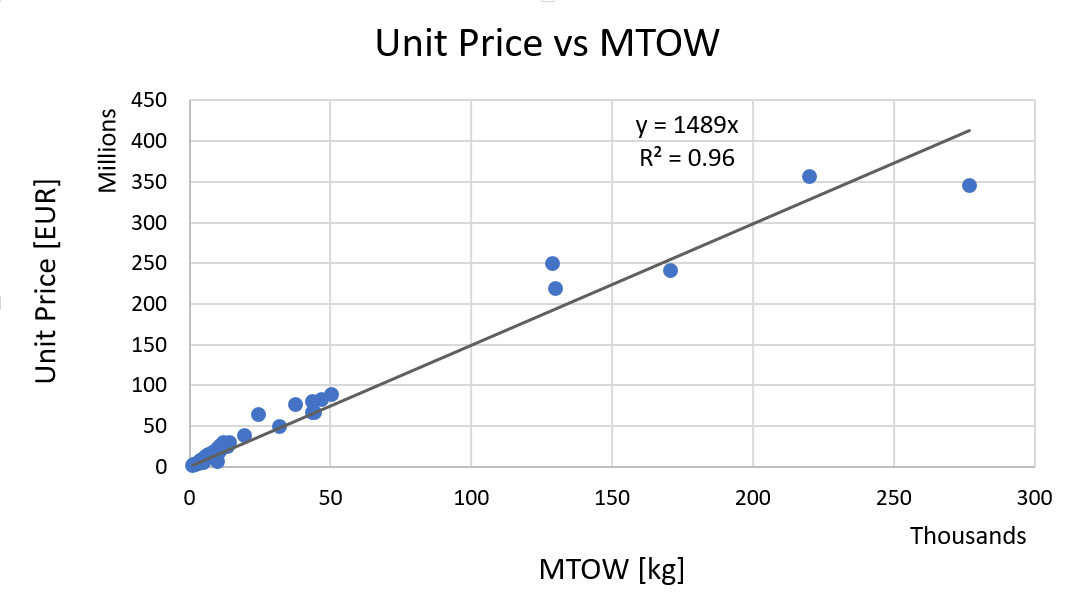
\includegraphics[width=0.6\textwidth]{CostAnalysis/Figures/Nomval}
    \caption{Relation between the unit price and the MTOW of conventional aircraft}
    \label{fig:nomvalgraph}
\end{figure}

The production cost of the nominal value is estimated in order to get a hunch of the magnitude of the cost. This is done by using statistical data of the nominal value: the conventional plane. In \autoref{fig:nomvalgraph}, the unit price of different aircraft is plotted against the Maximum Take-Off Weight (MTOW) of the aircraft. When a linear trend line, with intersecting point (0,0), is fitted to the data points, a relation is found between the unit price and the mass of the nominal value. Filling in the average mass of the Hybrid UAV concepts, being 52 kg, yields a unit price of around 77k EUR. Since there is a big difference in mass between conventional aircraft and the Hybrid UAV, one may wonder if this trend line can still be followed for masses in the order of 100 kg. This can be validated since aircraft of different mass categories, ranging from 1134 kg to 277000 kg, are used as data points while still having a very high $R^2$. \newline

Now, the unit price of the nominal value is estimated. However, the production cost is only a small part of the unit price. In general, the unit price consists of the profit, the development cost and the production cost. The profit per unit takes up around 5\% of the unit price \cite{costprofit}. The development cost per unit depends greatly on how many units are sold. Also the production cost per unit decreases with increasing amount of units sold. For the case of hybrid UAVs, it can be estimated that 80\% of the unit price goes to development cost since only few units are sold and many man-hours are spent into developing the concept. That leaves 15\% for the production cost. Using the unit prices estimated for the nominal value, a production cost of around 12k EUR is calculated.

\begin{figure}[H]
    \centering
    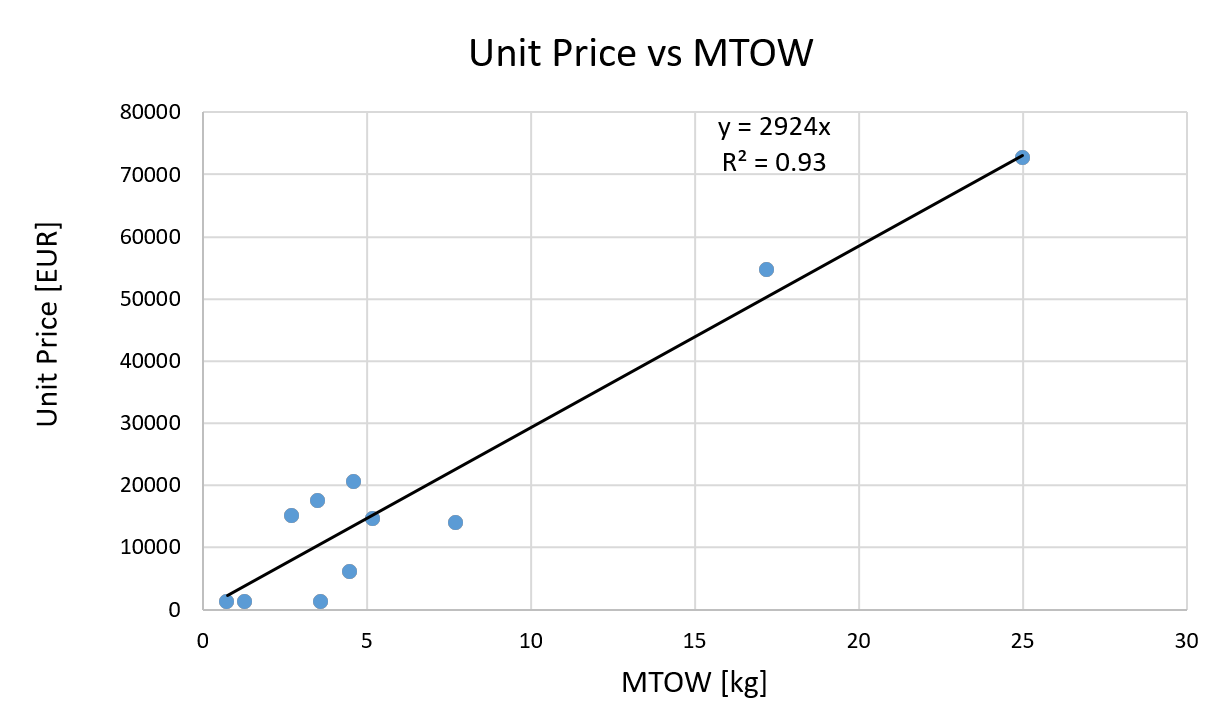
\includegraphics[width=0.6\textwidth]{CostAnalysis/Figures/CostEst}
    \caption{Relation between the unit price and the MTOW of hybrid and fixed wing UAVs}
    \label{fig:nomcost}
\end{figure}

A cost estimation for hybrid and fixed wing UAVs is also carried out in order to find out how the unit price of the nominal value will differ in price with an actual, similar UAV. In \autoref{fig:nomcost} the unit prices of hybrid and fixed wing UAVs are plotted against the MTOW. From the trend line, one can estimate a UAV of 52 kg to have a unit price of around 152k EUR. This number is significantly higher than the unit cost calculated with the conventional aircraft estimation, this can be explained by taking into account the non-recurring costs. The non-recurring cost per unit for aircraft will be much lower than  for UAVs since an aircraft will have much more units sold than UAVs which are typically designed for only one specific mission, e.g. killer drones, ambulance drones or surveillance drones. This means that for UAVs there will be more development cost per unit but also, to a lesser extent, more production cost. The production cost for UAVs will also be slightly higher than those of a conventional aircraft because UAVs generally include more features than a conventional aircraft, e.g. hovering capabilities or VTOL. From the unit price for a 52 kg UAV one can calculate that the production cost would be around 23k EUR. This estimation lies very close to the cost requirement stated by Avy.


\section{Concept Analysis}
\label{sec:conanal}
In this section, the five chosen concepts will be analysed for cost on five different criteria: the manufacturing cost, material cost, mechanism cost, power \& propulsion cost and weight influence on cost.  
\subsection{The Tailsitter}

\paragraph{Manufacturing Costs}\label{sec:tailmanu}

The Tailsitter scored two pluses in this category. The first reason is that it is missing a fuselage structure, this means that there is a big part not needed to be manufactured. In general, the fuselage takes up 28\% of the total manufacturing costs\footnote{https://ocw.mit.edu/courses/aeronautics-and-astronautics/16-885j-aircraft-systems-engineering-fall-2004/lecture-notes/pres\_willcox.pdf, Accessed 02-05-2017}. The next reason is the low complexity of The Tailsitter: it has no secondary curves. Because of this it is easy to manufacture seeming it does not need special tools and machines compared to the nominal value. Laminating and other processes that may be required can be done easily on these flat surfaces. The last dominating reason is that the assembly of this aircraft would be very simple. There are just three major parts in this aircraft (tailplane, engine and wing) which can be assembled without much difficulties.

There are also disadvantages: the first one being that the inside of the wing will be more complex because it will need more support structure than the nominal plane to carry all the loads. This will take up more time to manufacture, costing more man-hours. This disadvantage does not have as big of an impact as the advantages combined, causing The Tailsitter to keep its two pluses.


\paragraph{Material Costs}

Two pluses are scored by The Tailsitter for the material cost. The material costs will be lower than the nominal aircraft. The first reason is that there is no fuselage, skipping a lot of the materials required to keep such a structure to strength. The next reason is derived from the expected loading cases. The greatest forces that will be encountered by the Hybrid UAVs act when they are taking off, this aircraft however can handle this force pretty well. When this aircraft needs to take off, it will pull the whole aircraft by its nose, creating a pulling force on the structure. This pulling force can easily be absorbed by the structure because it will not create bending moments or other stresses besides the tension.

\paragraph{Mechanism Costs}

For mechanism costs, The Tailsitter scores two minuses. It has conventional control surfaces and no complex moving wings but the propellers are making the costs go up. The first reason for this is that the propellers are counter-rotating, requiring complex mechanisms which will be expensive to buy or manufacture. Besides this, the propulsion system will have a swash plate for control. This has a high cost which is not present in the nominal configuration\footnote{http://www.heli-factory.com/eng/accessories/taumelscheibe-heli-factory/index.php , Accessed 10-05-2017}$^,$\footnote{http://www.vortechonline.com/awparts/, Accessed 10-05-2017}.

\paragraph{Power \& Propulsion Costs}
The Tailsitter scores two minuses on power \& propulsion since it has only one engine with two counter rotating propellers. Using only one propeller is very cost inefficient, it costs twice as much as using four propellers as is explained in \autoref{sec:propcost}. If one engine is used, the engine costs 4k EUR calculated for a mass of 52 kg. Furthermore, the counter rotating propeller is 9-17\% more efficient but also has 27\% more acquisition cost than regular propellers \cite{vanderover}. This will make the propulsion part of the cost very expensive. The power subsystem costs less since the propellers are more efficient. Hence, less power is required to provide the same thrust.

\subsection{The Tandem}

\paragraph{Manufacturing Costs} The Tandem is expected to have high manufacturing costs, causing it to score one minus in this category. The wings of this aircraft have a complex bend at the end, which will require extra tooling and machines to manufacture it. This complex bend will also require more man-hours. Another reason is that the assembly will be complex because each wing has to be attached to the fuselage separately via the mechanisms.

\paragraph{Material Costs} This aircraft scores another minus on material cost. The reasoning behind this is that it needs high structural strength. The engines on the tip will cause a large bending moment requiring the wing to be stronger than usual. Also, the mechanisms holding the wings need to be very stiff and strong, because it will hold the wing by itself while still being able to rotate. Additionally, a bit more material will be needed for the surfaces of the aircraft, because it has a wing instead of a tail plane.

\paragraph{Mechanism Costs} The Tandem scores another minus. There are going to be four mechanisms on the aircraft, one for each wing, each attached to the fuselage on but a small area. These mechanisms need to be strong enough to withstand the loads that occur during flight, hence being big in size and strong in material. While being stiff and strong it should also be able to rotate the wings with no problems.

\paragraph{Power \& Propulsion Costs} The Tandem scores a plus for power \& propulsion. \autoref{propcost} explained how the number of engines affects the costs of the propulsion system, it has been concluded that having double the amount of engines will decrease the cost by $\sqrt{2}$. Seeming this aircraft has four engines, the cost for the engines will be low. Four propellers are also needed, but those costs are negligible compared to the engine costs. The power costs will be approximately the same as for a conventional UAV.



\subsection{The Prandtl Box}

\paragraph{Manufacturing Costs} The Prandtl Box received two minuses for manufacturing cost since it has a very complicated wing production and assembly. Also the fuselage mounted rotating engines increase the complexity of the manufacturing process. The wing will have to be made in separate parts which will have to be assembled together. Also the addition of the wing to the fuselage will be complex and will require high costs. 

\paragraph{Material Costs}
Two minuses are given to the material cost of The Prandtl Box. Due to the continuous wing being attached to the fuselage at two places, the forces acting on the wing will create strong bending moments in the fuselage \cite{pranbox}. In order to withstand the bending moments, the fuselage needs a strong structure. The material for the fuselage will therefore be more expensive. Also the material of the wing will be more expensive compared to the nominal value because the continuous wing has a large surface area . 

\paragraph{Mechanism Costs}
A plus is given to the mechanism cost of The Prandtl Box. The Prandtl Box only has fairly simple, rotating engines mounted at the fuselage as mechanism. Besides that, it only has conventional control mechanisms.

\paragraph{Power \& Propulsion Costs}
Another plus has been given to the power \& propulsion cost of The Prandtl Box. This is because The Prandtl Box uses four propellers which cost around 2k EUR which is only half the price for one propeller. The cost for power is more or less conventional for this concept.


\subsection{The Tiltrotor}

\paragraph{Manufacturing Costs} 
The Tiltrotor has zero points for the manufacturing costs. It has a conventional layout so when compared to the nominal aircraft there is not much difference in manufacturing. The only difference that arises is that the engines need to be assembled on the wingtips, but this does not much extra work.

\paragraph{Material Costs}
For the material costs it has two minuses. The Tiltrotor has a conventional design meaning that there are no extra surfaces that need material. But the engines on the tip of the wing are causing high bending moments. To support these forces the wing has to be strong and stiff enough, requiring more material which increases the cost by quite some bit.

\paragraph{Mechanism Costs}
The Tiltrotor has two minuses for mechanism costs. These minuses come from the complex swashplate that is needed for stability and control during hovering and the mechanisms needed to rotate the engines at the tip. Unlike other concepts, there are only two engines instead of four, this means that the weight of the engines is higher. This higher weight in turn means that the mechanisms need to be stronger, hence more expensive.

\paragraph{Power \& Propulsion Costs}
One plus is what The Tiltrotor gets for power \& propulsion. \autoref{sec:propcost} shows that two engines have a $\sqrt{2}$ times higher cost than four engines, hence only the one plus.


\subsection{The Winged Quadcopter}

\paragraph{Manufacturing Costs} 
The Winged Quadcopter was given a zero for manufacturing cost. The Winged Quadcopter design is very similar to a conventional plane. Only two beams with engines mounted on it, are mounted on the wings of the UAV. For manufacturing cost, adding the two beams to the design was considered to be fairly easy and low-cost.

\paragraph{Material Costs}
Again, a zero is given to The Winged Quadcopter for material cost. The design doesn't differ a lot from the nominal value. For material, only a few extra costs are present due to the beams added to the conventional design. The prices of those beams are estimated to be low.

\paragraph{Mechanism Costs}
Another zero is given for mechanic cost to The Winged Quadcopter. Mechanisms are needed in order to rotate the propellers for horizontal and vertical flight. During horizontal flight, the back propellers blades are also going to be folded together in order to decrease the amount of drag. The cost of these mechanisms are not considered to differ a lot from the nominal value since the mechanisms are not complex.  Some conventional control surfaces are also present on the wing and the tail.

\paragraph{Power \& Propulsion Costs}
A zero is given to the power \& propulsion cost of The Winged Quadcopter. The design uses the four engines for vertical flight, which is twice as cheap as using one engine. In horizontal flight, one engine on the nose is used plus two engines that rotate to the horizontal mode. Since this design uses five engines, it will cost more than the other concepts with only four engines but still less than the concepts with two engines.

    \chapter{Development Risk}
\label{ch:deve_risk}

It is important to assess the development risks associated with the various concepts as this gives important insight into the their feasibility. Development risks are the risks related to the development phase. Therefore, these are the risks of not being able to comply with the constraints, such as on time and money. In order to characterise the development risk associated with each concept, it is first necessary to identify a number of factors that are influential. These factors include:

\begin{enumerate}
    \item The level of feasibility of the concept. This depends on weather the concept has been proven and implemented before. 

    \item The level of complexity of component and elements contained in the concept. Does the concept contain systems or mechanisms that are not directly available at the moment, but require development or optimisation for this application? The required technology might still be in its infancy. Assessing this risk is thus of vital importance.
  
    \item The availability of knowledge or expertise related to a particular concept. This can be regarded as a development risk decreasing factor; the more available, the less risk there will be.
    
\end{enumerate}

\section{Concept Evaluation}

In the first subsection of this section the grading system will be elaborated on. the second subsection contains the grading table of the concepts with respect to development risk.

\subsection{Grading system} %maybe rephrase name
%These expected design obstacles can be expressed as risks that need to be assessed. 

A concept with a higher level of complexity has, by definition, less predictability. This means there is the risk that during the development unpredicted problems may show up; problems that cause the design to require more resources than prior foreseen. For instance, more time and money is needed to research certain unexpected phenomena and implement measures to counteract these.

What does this mean in practical terms for the case that a complex mechanism is incorporated in a design concept? In case the mechanism has not been used before, there is a substantial risk that the expected development resources needed will be more than prior estimated. This is due to the fact that there is no proof that the concept works. In the current concept selection, all the mechanism in the concepts do exist.  However, existing concepts might need optimisation for their application. A tandem rotating wing mechanism, for instance, has been used in aircraft design, but has seldom been implemented in a UAV application. Due to the level of complexity, which means higher uncertainty, this process might need more required resources as foreseen.

All the concepts will be analysed with regard to development risk in a qualitative way. For the quantitative approach a Technology Feasibility Scale (TFS) was created. This scale is inspired by the Technology Readiness Level Scale created by NASA\footnote{\url{https://www.nasa.gov/directorates/heo/scan/engineering/technology/txt_accordion1.html}, Accessed 22-05-2017}. By means of this TFS, a value can be attributed to the development risk of each concept.\\

\noindent The TFS, as portrayed in \autoref{fig:DRS}, has five different levels, labelled from A to E.

%no need for period in short itemise!
\begin{itemize}
    \item \textbf{A:} Commonly applied concept (0\% - 20\%)
    \item \textbf{B:} Concept with existing UAV applications (10\% - 40\%)
    \item \textbf{C:} Proven concept by means of working prototype (30\% - 60\%)
    \item \textbf{D:} Never applied, but theoretically feasible (50\% - 80\%)
    \item \textbf{E:} High risk that the concept is infeasible to develop (70\% - 100\%)
\end{itemize}

\begin{figure}[htb]
    \centering
    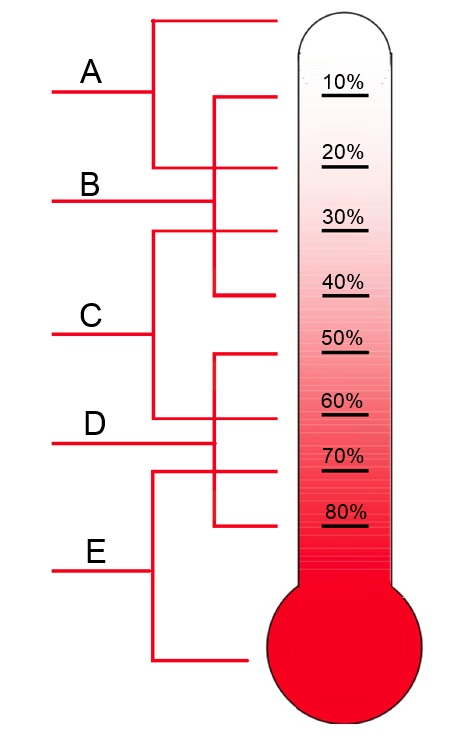
\includegraphics[width=.30\textwidth]{DevelopmentRisk/Figures/DRS.jpg}
    \caption{Technology Feasibility Scale}
    \label{fig:DRS}
\end{figure}

Next to the Technology Feasibility Scale, there are two other aspects that influence the total development risk. First, the level of complexity of the design; high complexity increases the development risk by an estimated percentage range of 0-20 percent. This value will be assigned to a concept based on the qualitative analysis, that can be found in \autoref{sec:qca}. The development risk is lowered if a knowledge source is available, which can assist the preventing of potential development stagnations. An example of this is the TU Delft tail sitter ATMOS, the expertise at the university decreases the development risk by an estimated percentage of 10 percent. 

\subsection{Grading of the concepts}

\autoref{tab:developmentrisk} shows the grading of the concepts. The percentages are shown in the different columns and by means of adding up, the development risk is obtained.

\begin{table}[H]
\caption{Concept Development Risk Grading}
\label{tab:developmentrisk}
\centering

\begin{tabular}{r|>{\centering}p{2.5cm}:>{\centering}p{2.5cm}:>{\centering}p{2.5cm}|c} 
\textbf{Concept \rotatebox{90}{\hspace{0.5cm}Criterion}} & \rotatebox{90}{\textbf{Feasibility [\%]}} & \rotatebox{90}{\textbf{Complexity [\%]}} & \rotatebox{90}{\textbf{Avail. Expertise [\%]}}  & \rotatebox{90}{\textbf{Dev. Risk [\%]}} 
    \\ \midrule

Tailsitter      & 25 & +10 & -10 & 25 
\\ \hdashline
Tandem          & 50 & +15 & 0 & 65 
\\ \hdashline
Prandtl Box     & 35 & +5 & -10 & 30 
\\ \hdashline
Tiltrotor       & 40 & +15 & 0 &  55
\\ \hdashline 
Winged Quad.    & 5 & 0 & 0 & 5
\\ \bottomrule
\end{tabular}

\end{table}


%%%%%
%Quality control Kelbey till here
%%%%%

\section{Qualitative Concept Analysis}
\label{sec:qca}
In this section, each concept will be analysed based on how much inherent development risk is present. Each concept will be analysed based on the grading system laid down in the previous section.

\subsection{Concept 1: The Tail sitter}
The Tailsitter is a proven concept; there are working prototypes and even some models available on the market. One can think about the ATMOS UAV\footnote{\url{http://www.atmosuav.com/}, Accessed 22-05-2017} and the DelftaCopter\footnote{\url{http://www.delftacopter.nl/delftacopter/}, Accessed 22-05-2017}. For this reason, this concept is classified as a category B on the Technology Feasibility Scale. 

There are no complex mechanism, like rotating parts, to be incorporated in the design that might induce any other development risk. However, there is some increase in risk due to the need for a complex control system in the transition phase from vertical to horizontal flight. This is included as a 10\% risk increase. For solutions to problems that occur, one of the existing designs can be consulted. Added to that is the fact that the TU Delft has a lot of expertise in the field of hybrid UAV Tailsitter concepts. This is included in the form of a development risk reduction of 10\%, which cancels out the 10\% increase caused by the control system. Due to the expertise and knowledge available at TU Delft, the development risk associated with designing the control system can be offset. 

\subsection{Concept 2: The Tandem}
This concept comprises three key elements which need to be examined when considering the development risks associated with it. 

The first element is the tandem wing configuration. Concepts and prototypes of hybrid UAVs using this wing configuration do exist; an example is the Airbus’s Quadcruiser UAV.  The second key element of this design is the use of four rotors for both VTOL and for horizontal flight. This is the most common configuration for VTOL UAVs because of the good stability and manoeuvrability this configuration offers. There is little development risk associated with utilising a quad-rotor.
The rotating wing Hybrid UAV concepts has been proven to be a feasible concept (The Greased Lightning GL-10\footnote{\url{https://www.nasa.gov/langley/ten-engine-electric-plane-completes-successful-flight-test}, Accessed 24-05-2017}). However, the rotating wing and the mechanics it introduces will cause a higher level of complexity. The level of complexity of the rotating wing is even considered higher than the level of complexity of just a tilt rotor \cite{princeton}. Like stated in the introduction of this chapter, extra complexity will increase the development risk. In this case, the net effect is an risk increase of 15\%.

So far as literature study goes, no commercially available UAV which resembles this concept was found. There is, however, one concept under development which does combines the three key elements. GH Craft, Japan is developing a tandem, rotating wing UAV demonstrating that this concept possesses some degree of feasibility\footnote{\url{http://www.ghcraft.com/QTW/QTW-UAS.htm}, Accessed 22-05-2017}. It is therefore classified as a Category C concept but towards the high risk end of the said category for the reasons mentioned above.

\subsection{Concept 3: The Prandtl Box}
Elements that are relevant to consider with regard to development risk are the rotating motors and the Prandtl wing box. The rotating motors contain mechanisms that introduces complexity to the design. There is the risk that the development of those systems to the point that they perform adequately might require more resources than foreseen. This is included in the grading as a risk increase of 5\%.

Although the Prandtl box concept is currently not used in general aviation, it is a proved concept. The AVY concept also incorporates the Prandtl wing box in their UAV design \footnote{\url{http://www.avy.eu/}, Accessed 11-05-2017}. This means that the development risks of this concept are limited; the chance that using this concept in the design will result in an unexpected resource requirements or even turns out to be unfeasible is unlikely. Due to the fact that AVY has a working prototype, and there are other Prandtl box configurations, this concept is classified as a Category C on the Technology Feasibility Scale. The value assigned to this concept is on the low end of this Category, namely 35\%.

\subsection{Concept 4: The Tiltrotor}
The Tiltrotor concept has been used before in both manned aerial vehicles and UAV applications. Aerial vehicles with a tiltrotor configuration are the V-22 Osprey and Bell Eagle Eye. Since this concept has been implemented successfully, The Tiltrotor is considered a category B on the Technology Feasibility Scale, but towards the high risk end of this category (namely 40 \%) because of the low number of tiltrotor UAVs on the market.                                   
The Tiltrotor concept presents a seemingly straightforward concept characterised by a conventional configuration with rotatable motors at the ends of the main wing. It seems that the complexity of this concept is quite low, but the opposite is true. 

Key to the success of this concept is a very advanced control system which must be meticulously developed and extensively tested. This control system is required to maintain controllability especially during the transition from vertical flight to horizontal flight as well as during hovering. The risk associated with not being able to develop an adequate control system capable of meeting the requirements is therefore large. Furthermore, an important factor in assessing the development risk is characterising the cost of development typical of such a design. The fact that this concept only has two rotors means that the controllability is substantially more difficult. Assuming that a control system capable of meeting the control requirements can be developed, substantial cost will be associated with developing it. The complexity of the control system translates into a large number of man-hours required for development and testing increasing the cost associated with the development. In the grading this is taken into account by a risk increase of 15\%.

In order to accomplish a successful design, thought needs to be given to what systems are necessary. The fact that there are only two rotors increases the required complexity of the design even further. In the event of one motor failing, the choice whether or not to include redundancy is an important factor in the level of development risk associated with this concept. If a redundant system is chosen, a complicated drive axis system would be required such that each motor can drive the other in the event of a failure. The development risk associated with this is large. 

\subsection{Concept 5: The Winged Quadcopter}
The Winged Quadcopter merges a conventional configuration airplane with a quadcopter. This is the most basic hybrid UAV concept and as a result has very little development risk. Due to the conventionality of this concept, it is classified as a category A on the Technology Feasibility Scale and has a assigned percentage of just 5\%.

There are many Hybrid UAVs on the market that utilise this or a very similar concept. This is an indication of the technical feasibility as well as the ease of development associated with this concept. Complexity is introduced by adding the capability of rotating the rotors in order to make use of them in both flight regimes (vertical \& horizontal). This increases not only the mechanical complexity but also the complexity of the control system and thus increasing the development risk.

Nevertheless, conventional configuration UAVs with four tilt rotors are commercially available. Quantum Systems develops and sells such a concept proving the technical and commercial feasibility of such a concept\footnote{\url{https://www.quantum-systems.com/}, Accessed 24-05-2017}. This indicates that the development risk linked to concept 5 is moderate to low and can thus be quantified so low that it can be neglected.


    \chapter{Sustainability Analysis}
\label{ch:sustain}
\setlength{\parindent}{15pt}
%Brian Joel Chris

Sustainability is an important aspect that should be considered as a trade-off criterion. A system has an impact on its environment for its entire life cycle. Sustainability has an environmental, social and economical aspect. In order to evaluate sustainability of each concept, a clear definition of a sustainable design is formulated as following:


\begin{displayquote}
\textit{Sustainable Design is defined as an Unmanned Aerial System design which has low environmental impacts throughout its life cycle, from design phase until end-of-life phase.}
\end{displayquote}


All three aspects should be assessed to have a solid sustainability analysis. However, only impacts in the environmental aspect will be assessed, as impacts on the social aspect are assumed to be same for all concepts; for instance, residents of a city may feel insecure  and unhappy due to UAVs flying over their houses. Impacts on the economical aspect are assessed in \autoref{ch:costanal}, so they will not be assessed in this chapter. 

\section{Sustainability Trade-Off}

In this section, the sustainability trade-off performed in the whole chapter is analysed. First, a summary of the final results is presented in \autoref{tab:costsubtrade}. Then, the grading system that has been used is explained.  

\subsection{Summary}

In this section, a summary regarding the sustainability performance is given in \autoref{tab:sustrade}. It can be seen that The Winged Quadcopter and The Tailsitter score best in terms of sustainability. This comes due to their low noise emission compared to tilt-rotor concepts for example. Also the materials used have a lower carbon footprint and cumulative energy demand. 
It can also be noted that The Tandem is the worst in terms of sustainability. This is due to the higher noise emissions and bad manufacturing performance.

Regarding the weights, the manufacturing trade-off has obtained a weight of 67\% while the noise emissions have obtained only 33\%. The reasoning behind this is that the noise emission have only been evaluated qualitatively, while the manufacturing trade-off makes use of numerical values to compare the concepts. 

\newcolumntype{C}[1]{>{\centering\let\newline\\\arraybackslash\hspace{0pt}}p{#1}}
\begin{table}[H]
    \centering
    \caption{Sustainability Sub Trade-Off}
    \label{tab:sustrade} 
    \begin{tabular}{r|>{\centering}p{3.3cm}:>{\centering}p{1.6cm}|c} 
    \textbf{Concept \rotatebox{90}{\hspace{0.5cm}Criterion}}         & 
    \rotatebox{90}{\textbf{Manufacturing}}                           & 
    \rotatebox{90}{\textbf{Noise Emissions}}                         &
    \rotatebox{90}{\textbf{Outcome}} 
    \\ \midrule
    The Tailsitter         &  ++  &    0   & 83.5 \% 
    \\\hdashline
    The Tandem           & -     &    -        & 25\% 
    \\\hdashline
    The Prandtl Box        &    0 &   +        & 58.25\% 
    \\\hdashline
    The Tiltrotor          & -    &     \texttt{-{}-}    & 16.75\% 
    \\\hdashline
    The Winged Quad.       & ++    &   0       & 83.5\% 
    \\ \midrule\midrule
    Weight             & 67    & 33        &  
    \end{tabular}
\end{table}

\subsection{Grading System}

There are two criteria for sustainability analysis. It is assumed that manufacturing criteria is twice as important as noise emissions criteria. Due to the differences in analysis for both criteria, a quantitative analysis with calculations is carried out for manufacturing criteria while a qualitative analysis with literature study and estimations based on engineering intuition is carried out for noise emissions criteria. Thus, the manufacturing criteria receives 67\% and the noise emissions criteria receives 33\%. Rating of trade-off is explained in \autoref{tab:susweight}.

\begin{table}[htb]
\centering
\caption{Definition of sustainability grading system}
\label{tab:susweight}
    \begin{tabular}{ccc}
        \toprule
        \textbf{Rating}           & \textbf{Meaning: manufacturing} &\textbf{Meaning: noise emissions}
        \\ \midrule
         ++            &    \textit{not used}     & Excels
        \\ \hdashline
        +               & No CED and CO$_{2}$ & Lower
        \\ \hdashline
         0          & Low CED and CO$_{2}$ & Average
        \\ \hdashline
          -           & High CED and CO$_{2}$ & Higher 
        \\ \hdashline
         \texttt{-{}-}    & \textit{not used} & Unacceptable
        \\ \bottomrule
    \end{tabular}
\end{table}


\section{Manufacturing}

In order to calculate the Cumulative Energy Demand (CED) and the carbon footprint of the different materials, the structural weight of each concept has to be assessed. For this, it is assumed that the structural weight is 20\% of the maximum take-off weight. For a robust carbon footprint and CED analysis this can be assumed, as only the relative difference between the designs matters for the trade-off.

\paragraph{The Tailsitter} This concept will be constructed with a polymer foam, according to the pattern set by ATMOS UAV systems. This can be a foam like Expanded Polypropylene (EPP)\footnote{\url{http://www.atmosuav.com/ufaqs/materials/}, Accessed 19-05-2017} 
EPP has the property that it is convenient and environmentally friendly to recyclable. During recycling it does not emit harmful gasses\footnote{\url{http://www.intcorecycling.com/how-to-recycle-epp.html}, Accessed 19-05-2017}.

\paragraph{The Tandem} Due to the bi-directional loads that are exerted on the wings, composites will most likely not be the chosen material. The wing is both used for lift generation, engine supporting and for impact absorption during landing. The chosen material will either be aluminium or EPP foam. Both aluminium and EPP foam are, in contrast to composites, easily disposed and can even be recycled. However, due to the higher allowable stresses for aluminium, this material will be used for the preliminary design.

\paragraph{The Prandtl Box} Due to the fact that the Prandtl Box is a complex structure, the stress analysis of it is a critical part. As Aluminium metals have a higher yield stress than polymers, it is for now assumed that the structure of the Prandtl Box is made out of aluminium. This make The Prandtl Box recyclable and gives it good manufacturing sustainability properties. 

\paragraph{The Tiltrotor} The wings of The Tiltrotor need to be strong and stiff enough to carry the loads and weight of the engines. This makes the use of polymer material inappropriate due to their low strength. Furthermore the engines will create loads in two direction, horizontally and vertically, hence composites materials are also not favourable. A metal alloy like aluminium is used as final choice. This makes The Tiltrotor recyclable and reusable.

\paragraph{The Winged Quadcopter} The wing of The Winged Quadcopter will not use composites due to drilling holes or joining parts. Either metal or EPP in combination with a metal structural element is viable for this concept. As the loads of this concept are assumed smaller than The Tandem, EPP will be used in this case.\newpage

The structural mass, carbon footprint and cumulative energy demand are summarised in \autoref{tab:manufac}. The carbon footprint and CED are calculated using US Life Cycle Inventory Database version October 2013 \cite{USLCI}. All EPP parts are assumed to be polypropylene resin and all aluminium parts are assumed to be smelt first then rolled, as aluminium sheets can be used to manufacture structural parts of UAV concepts.

\begin{table}[htb]
    \centering
    \caption{Carbon Footprint and Cumulative Energy Demand per Concept}
    \label{tab:manufac}
    \resizebox{\textwidth}{!}{
    \begin{tabular}{lcccc}
            \toprule
            \textbf{Concept}&\textbf{Total Mass [kg]} & \textbf{Structural Mass [kg]} &\textbf{CED [MJ]} & \textbf{Carbon Footprint [kg]}\\
            \midrule
            The Tailsitter   & 52 & 10.4 & 782 & 12.6\\\hdashline
            The Tandem       & 80 & 16   & 2986 & 266\\\hdashline
            The Prandtl Box  &  38& 7.6  & 1419 & 114\\\hdashline
            The Tiltrotor    & 75 & 15   & 2800 & 250 \\\hdashline
            The Winged Quad. & 44 & 8.8  & 662 & 10.7\\ 
            \bottomrule
    \end{tabular}}
\end{table}


\section{Noise emissions} 

Detailed calculation of noise emissions in this stage of the design phase is not possible. For this reason, the concepts regarded as having a nominal noise emission are discarded in the following discussion and are regarded as reference values in the trade-off. Then, the exceptional configurations are analysed with respect to the reference concept. An in-depth analysis of noise emissions also requires the discussion of the different types of noise. For example, animals may be affected by different types of frequencies, while people are in general irritated by higher frequencies. 

\paragraph{The Tailsitter} It uses a general flying wing shape as the design. This will not create any flow interference and hence not a lot of noise is generated due to the general aerodynamics. However, two counter rotating double propellers are used for propulsion. Due to interferences in counter-rotating propellers, the noise will increase significantly \cite{vanderover}. As these two propellers will have a higher intake area then The Winged Quadcopter, they will have a lower angular speed, which will reduce the noise again. In the end, it is assumed that the noise will be equal to the noise of The Winged Quadcopter.  

\paragraph{The Tandem} It has two wings and four engines; front and rear engines are not in line, however, increased flow interference will occur. This will result in an increase in noise. 

\paragraph{The Prandtl Box} Its wing configuration has a lower noise emission than conventional aircraft \cite{prandtl_noise}. Considering the propulsion system, four engines are used to generate thrust, which is similar to the reference design. Hence the noise level of The Prandtl Box is decreased compared to the general reference.

\paragraph{The Tiltrotor} It is highly impractical in terms of noise. Civil applications of a tiltrotor-type aircraft are limited due to this general known problem \footnote{\url{https://rotorcraft.arc.nasa.gov/Research/Programs/tramprogram.html}, Accessed 19-05-2017}. 


\paragraph{The Winged Quadcopter} It is assumed to have a nominal noise level.




\section{Other aspects} %these are just stated but not included in trade-off, assumed to be constant

Besides the manufacturing and noise emissions, each concept introduces issues related to sustainability. Although they are important and have to be taken into account in the final design, they are not part of this trade-off due to the fact that they are assumed to be equal for each subsystem. Several of these aspects are listed and explained in this section. 

First, transport of the UAV parts has to be taken into account. Depending on where a part is produced, it might have to be transported to another location for further processing. This will increase the carbon footprint of the design. For now however, all concepts are assumed to be manufactured at the same location under the same transport circumstances.

Then, reusability of the drone is also an important subject to be accounted for. A cracked wing of a drone might easily be replaced without having to create a new one. This is mainly dependant on how the drone is assembled and whether each subsystem can easily be removed. For the conceptual phase of the design, this is assumed to be constant. 

Finally, the social aspect of each concept is assumed to be same. As mentioned earlier, inhabitants living near a flying area can feel insecure or unhappy. Appearance of UAVs will not matter to the inhabitants, so the social aspect is negligible for a trade-off.
 









    \chapter{Ground Handling}
\label{ch:grou_hand}
%don't change this label again, whoever did this please just use the conventions (for a chapter --> ch:four letters of each word separated by underscores

In this chapter, the different aspects of ground handling of the UAV concepts will be discussed. This consists of all relevant stages before and after flight. The stages can be identified as assembly, transport (of the UAV) and storage related aspects dimensions and mass, payload mounting and maintenance. 
It is assumed that all concepts use a same type of ground system. Details about the ground system are elaborated in \autoref{sec:ol}. Also, it is assumed that charged batteries are available at any time such that used batteries after flight can easily be replace with charged ones. As a result, a ground system and batteries do not pose extra constraint on ground handling time. %An overview of different aspects of ground handling per concept is given at the end of this chapter.

%This chapter did not adhere to the standard structure, is it possible to change it to fit it that way?
% X Ground Handling
% X.1 Trade-Off
% X.1.1 Summary
% X.1.2 Grading System
% X.2 Criteria
% X.2.1 Criteria #1 < explain a bit how it influences
% etc
% X.2.X Criteria Weights
% X.3 Concept Analysis
% X.3.1 Concept 1 < here you explain how much + or - each concept gets for each criteria
% etc

\section{Trade-Off}
\label{sec:grou_hand_TO}
In this section, the difference in the concept's quality with respect to the several ground handling aspects are explained.

\subsection{Summary}
Each of the aspects have been given weights that represent their importance to ground handling, as can be seen in \autoref{sec:grou_crit}. In \autoref{tab:summ_grou_hand} the performance of each concept is summarised. 

% The dimensions have the lowest weight, as these only influence in what type of vehicle the UAV can be transported. The mass influences both transport, but also the ease with which the UAV can be handled. On the other hand, during maintenance it would not be possible for any of the designs to just lift it up with one person in any case, which resulted in the relatively low weight for mass. 
%Payload mounting is very important yet does not have the largest weight, as the mounting concept can easily be changed for all of the designs.
%Then both the assembly and maintenance have been assigned the largest weights, since they make up most of the time of the ground handling and are crucial to the success of the missions.


The concepts that perform best in terms of ground handling are the Tailsitter and the Winged Quadcopter. It can be seen that both of them perform well in terms of mass and payload mounting. The worst concept, in terms of ground handling, is the Tandem.

\begin{table}[]
    \centering
    \caption{Ground Handling Sub Trade-off}
    \label{tab:summ_grou_hand}
    \begin{tabular}{r|>{\centering}p{2.5cm}:>{\centering}p{1cm}:>{\centering}p{1.25cm}:>{\centering}p{2cm}:>{\centering}p{2.5cm}|c}
    \textbf{Concept \rotatebox{90}{\hspace{0.5cm}Criterion}}            & 
    \rotatebox{90}{\textbf{Assembly}}                                   &
    \rotatebox{90}{\textbf{Dimensions}}                                 & 
    \rotatebox{90}{\textbf{Mass}}                                       & 
    \rotatebox{90}{\textbf{Payload mounting}}                           & 
    \rotatebox{90}{\textbf{Maintenance}}                                &
    \rotatebox{90}{\textbf{Outcome}}
    \\ \midrule
    Tailsitter      &  +    & - -   &  +     &  + +  &   -   & 60\% 
    \\\hdashline
    Tandem          & - -   & + +   &  -     &   0   &   0   & 38\% 
    \\\hdashline
    Prandtl Box     &  0    & + +   & + +    &   -   &   +   & 54\% 
    \\\hdashline
    Tiltrotor       &  -    & -     &  -     &  + +  &  0    & 51\% 
    \\\hdashline
    Winged Quad.    &  +    & 0     & + +    &  + +  &  +    & 82\% 
    \\ \midrule\midrule
    Weight          & 27    & 10     & 15   & 21    & 27    &  
    \end{tabular}
\end{table}

\begin{comment}
\begin{table}[]
    \centering
    \caption{Ground Handling Sub Trade-off}
    \label{tab:summ_grou_hand}
    \begin{tabular}{r|>{\centering}p{2.5cm}:>{\centering}p{0.5cm}:>{\centering}p{1.25cm}:>{\centering}p{2cm}:>{\centering}p{2.5cm}|C}
    \textbf{Concept \rotatebox{90}{\hspace{0.5cm}Criterion}}            & 
    \rotatebox{90}{\textbf{Assembly}}                                   &
    \rotatebox{90}{\textbf{Dimensions}}                                 & 
    \rotatebox{90}{\textbf{Mass}}                                       & 
    \rotatebox{90}{\multicolumn{1}{p{2cm}}{\raggedright \textbf{Payload mounting}}}  & 
    \rotatebox{90}{\textbf{Maintenance}}                                &
    \rotatebox{90}{\textbf{Outcome}}
    \\ \midrule
    Tailsitter      &  +    & - -   &  +     &  + +  &   -   & 60\% 
    \\\hdashline
    Tandem          & - -   & + +   &  -     &   0   &   0   & 38\% 
    \\\hdashline
    Prandtl Box     &  0    & + +   & + +    &   -   &   +   & 54\% 
    \\\hdashline
    Tiltrotor       &  -    & -     &  -     &  + +  &  0    & 51\% 
    \\\hdashline
    Winged Quad.    &  +    & 0     & + +    &  + +  &  +    & 82\% 
    \\ \midrule\midrule
    Weight          & 27    & 10     & 15   & 21    & 27    &  
    \end{tabular}
\end{table}
\end{comment}

\subsection{Grading System}

The grades given are based on a better and worse performance. In \autoref{tab:grad_grou_hand}, the grading system can be found.
\begin{table}[]
    \centering
    \caption{Definition of ground handling grading system}
    \label{tab:grad_grou_hand}
    \begin{tabular}{r l}
    \toprule
     Rating    & Meaning 
     \\ \midrule
     + + & Excels 
    \\ \hdashline
    + & Better
    \\ \hdashline
    0 & Average
    \\ \hdashline
    - & Worse
    \\ \hdashline
    - - & Bad
    \\ \bottomrule
    \end{tabular}
\end{table}



\section{Criteria}
In this section, each of the criteria that is used in the ground handling sub-trade-off is discussed.

\subsection{Assembly}
In this section, the assembly advantages and disadvantages of each concept are discussed. Assembly has been given the largest weight as it makes up most of the time spent during ground handling. It is also very important as unsuccessful assembly will most likely lead to mission failure.


\paragraph{The Tailsitter} 
The Tailsitter does not have a separate fuselage section since it is a flying wing design. Because of this, there are only two parts that would naturally have to be assembled later. The propeller and the tail section can be removed to make transportation easier. It is also possible to section the wing. However, this will have a large negative impact on the structural integrity of the Tailsitter and impose a weight penalty because the connectors have to be rigid.


\paragraph{The Tandem} 
The Tandem poses an issue regarding the ease of (dis)assembly. This is because the propulsion is directed vertically by rotating the entire wings instead of rotating the propellers. Since joints have to withstand high stress while being able to rotate, it requires stiff assembly. On the contrary, the propellers do not require reinforced joints. 
Although there are several disadvantages, The Tandem does not have a tail, which reduces the assembly stage. 

%Since the connection already has to be able to endure a lot of stress while also being able to rotate, it requires the assembly to be very stiff. On the other hand, the propellers do not require an extra connection. The assembly of the propellers can therefore be done easily. The Tandem does not have a tail, meaning there is one less part to assemble. 



\paragraph{The Prandtl Box} 
The Prandtl Box has multiple options for assembly. An advantage of The Prandtl Box is that it can be deconstructed for easy transport. For the assembly of the wing, it should be kept in mind here that the closed wing section provides structural integrity. The wing will be disassembled into  straight pieces and corners, where the last ones are connection pieces. This is done because it will allow for easier transportation. Easy assembly of the wing requires the wing material to have some elasticity since the wing section is closed.
All of the propellers can also be disassembled from the fuselage. It might even be possible to store everything inside the fuselage during transportation. This would, however, something to be considered during a later design stage.


\paragraph{The Tiltrotor}
The Tiltrotor has a similar problem as the Tandem has in assembly. The rotating propellers pose a weakness in the structure, and the connection has to be able to endure a lot of stress. But as the bending moment in the connection will be smaller, stresses won't be as high. This poses less restrictions on the connection type, making assembly less complex. It is also possible to only require the assembly of the tilting mechanism once, and make it possible to remove the wings and the propeller blades for transportation. The tail could also be disassembled, depending on the size of the transport vehicle.


\paragraph{The Winged Quadcopter}
The Winged Quadcopter design enables easy dis-assembly for transport, since the different components have a lot of natural assembly points. The assembly might take slightly longer than that of other concepts, because of this large number of assembly points. It will be possible to disassemble the wings, rotor blade mechanism and tail. A large advantage is that it is not necessary to disassemble the rotor blades once assembled as the entire mechanism can be taken off.



\subsection{Dimensions}
In this section, the dimensions of each concept are compared. This is done because different dimensions might influence the possibilities of transport and handling. Both the dimensions in the fully assembled and disassembled case are discussed. The estimated dimensions are based on the wing size estimation, as can be found in \autoref{sec:geom_prop}, and on the payload requirement that determines the fuselage size (SYS-PH-1.2). The wing thickness was not determined yet, but has been assumed equal to 10 cm, based on a chord of 0.66 m and a t/c ratio of 15\%\footnote{\url{http://www.wseas.us/e-library/conferences/2008/cairo/CD-MECHANICS/MECHANICS17.pdf}, Accessed 18-05-2017}. Both of these are overestimated, which means the actual design will probably have wings a lot thinner than 10 cm. 
Based on average vans and cars, it is determined whether transportation is possible or not.\footnote{\url{https://www.businbedrijf.nl/nl/productinformatie/autogegevens/volkswagen}, Accessed 18-05-2017}$^{,}$ \footnote{\url{http://www.autoweek.nl/forum/read.php?1,5365747}, Accessed 18-05-2017} Since the dimensions only influence the possibilities of storage and transport of the UAV, it has been assigned a very small weight.



\paragraph{The Tailsitter}
The Tailsitter is estimated to fit in 2.60 x 1.10 m, based on the wing span and the payload orientation. This means it can never be transported in the back of a car, and only in certain vans. Only the propeller and the tail are disassembled in that case.

\paragraph{The Tandem}
The Tandem has an estimated wing span of 2.74 m, which means that without dis-assembly, it has the same problems as the Tailsitter yet can be transported in some vans. Even though assembly of the Tandem is not very easy, it is possible. Since the wing width is estimated at 42 cm, the Tandem should fit in 0.42 x 1.10 m, with a height of 55 cm. The propellers take up an additional 1.00 x 1.00 x 0.40 m as there are four. It is possible to transport this in any van or in a car with a large trunk. 

\paragraph{The Prandtl Box}
The Prandtl Box can be deconstructed to a large extent, meaning it can be made to fit into smaller dimensions. The total wing area is estimated to fit into 1.60 x 0.45 x 0.70 m, the fuselage section in 1.20 x 0.50 x 0.50 m and the propellers in 50 x 50 x 50 cm. This means it is possible to transport the Prandtl Box in any van or a car with a large trunk. 


\paragraph{The Tiltrotor}
The Tiltrotor is estimated to fit into 1.80 x 0.50 x 1.00 m for the wings and rotors plus tail and 1.20 x 0.50 x 0.50 m for the fuselage part. That means the dimensions are such that it can probably not be transported in a car. A van is required, but most are compatible. 


\paragraph{The Winged Quadcopter}
The Winged Quadcopter can fit into 1.70 x 0.50 x 0.50 m for the wings plus rotors and 1.20 x 0.50 x 0.50 m for the fuselage plus tail. This means it can be transported in some cars and in most vans.



\subsection{Mass}
In this section, the influence of the estimated mass with respect to ground handling is discussed. The mass estimations of each concept can be found in \autoref{sec:mass_esti}. Since recommended safety limits for carrying weight say women should carry max 16 kg and men 25 kg\footnotemark, a smaller mass means ground handling can be done with less people. When the mass gets too big, it might even be necessary to use a lifting device. This would impose a large penalty on the ground handling. Smaller mass enhances the general ground handling because it makes a lot of aspects like payload mounting and maintenance easier.
\footnotetext{\url{http://www.beckettandco.co.uk/manual-handling-faq-weight/}, Accessed 16-05-2017} As mass influences a lot of the other criteria and can partly be seen in those scores, it has not been given a large weight.



\paragraph{The Winged Quadcopter and the Prandtl Box} are estimated to weigh 44 and 38 kg, respectively. This makes it possible to be carried by two people when they're all men or three people. This is a great advantage in transport, since handling is really easy.

\paragraph{The Tailsitter} is estimated to weigh 52 kg, requiring three to four people to carry it. As the UAV is not that large, it is not desirable to require over four people. This is because it becomes harder to hold it with more people. 

\paragraph{The Tandem and the Tiltrotor} are both expected to have a weight around 80 kg, requiring four to five people to handle it. This is still possible, but not very desirable in terms of ground handling.


\subsection{Payload Mounting}

The payload mounting is relevant for the ground handling because faster mounting means faster ground handling. The mounting concepts can be divided into different groups: ones making use of a clicking mechanism, and ones using a door. These groups can then be divided in easy accessible doors or openings and openings that are located on, for example, the bottom of the UAV. The payload mounting has been assigned a weight close to the average weight, larger than mass and dimensions but smaller than the other two, because it is one of the most important aspects and has a very large impact on ground handling time, yet the system can easily be changed for each concept.

The clicking mechanism makes payload mounting very easy as it only requires the payload module to be clicked into the UAV, taking only seconds. For the Tailsitter, Tiltrotor and Winged Quadcopter, this mounting mechanism is used. For each concept, however, the payload is loaded through the bottom of the UAV when it is stored. This is because the UAVs are all in the same position when the payload is installed as they are while hovering, and the payload mounting method should enable dropping of the payload. There is no system that allows both just sitting on the ground or a table while being loaded.

The door system requires extra work, and therefore is not as beneficial as the clicking system. Both the Prandtl Box and the Tandem make use of it. The difference, however, is that the Tandem can be loaded while sitting on its landing gear while the Prandtl Box has to be loaded through the bottom when in storage. This gives the Tandem an advantage over the Prandtl Box.





\begin{comment}
I took this out, it's just a comment since I didn't want to remove all of it straight away x steph

For a successful mission performance, it is very important that the payload can be carried reliably. The reliability of the payload mounting system can be assumed equal for each design, however some designs are more susceptible to centre of gravity variation. 

The Tandem, Winged Quadcopter, Prandtl Box and Tiltrotor each have a larger range of stable centre of gravity positions. This is due to the fact that they either have wings or tails at the back for stability purposes. Since the tandem concept has no tail, the others have an advantage over it in terms of stability.

The tailsitter concept however is a based on a flying wing design. One major disadvantage of flying wings is the allowable range of centre of gravity. This can become a reliability concern which can be solved using a fixed payload bay. In addition to this, the payload has to be distributed equally over the payload bay in order to not shift the centre of gravity. 
\end{comment}










\subsection{Maintenance}


The ease with which maintenance can be performed on the different designs is dependent on multiple factors that were already discussed, like weight and assembly, but also on thinks like accessibility. Looking purely from a maintenance perspective, some parts are just easier to replace than others. This will be discussed in this section. The maintenance has been assigned the largest weight along with assembly since it makes up most of the time of the ground handling and is vital to the success of missions.

\paragraph{The Tailsitter} is potentially one of the hardest concepts in terms of maintenance. This is because it has such a large continuous wing area, which means it is impossible to replace parts. On the other hand, the stresses on the wing are not very large, meaning the repair might still be done using patches. The only parts that can be replaced are the tails, control surfaces and the propeller. The thin body and small payload opening also make maintenance on the inside harder, as it is less accessible. 


\paragraph{The Tandem} makes maintenance easier that the Tailsitter does since  it has multiple different parts. Each of these parts are easily accessed and replaced of serviced. The door on the back of the fuselage makes it possible to access the inside without lifting the UAV, but makes it hard to perform maintenance on the inside of the fuselage further to the front. 

\paragraph{The Prandtl Box} is a design that allows for relatively easy maintenance because of the large amount of parts that are assembled. This causes the maintenance of parts to be easier and cheaper, as they have small sub-parts. The large door on the bottom of the fuselage also allows for good accessibility, enhancing the possibilities of maintenance inside the fuselage.

\paragraph{The Tilt-Rotor} does not have as many sub-parts and has large weights on the edges of the wings, which means that it is not possible to do a repair in a lot of cases. Then the entire wing or other would have to be replaced, to maintain the structural strength. On the other hand, the large opening on the bottom makes maintenance on the inside of the fuselage easy.

\paragraph{The Winged Quadcopter} is somewhere between the Prandtl Box and the Tilt-Rotor in terms of easy maintenance. This is because it has a lot of removable parts, but not as many as the Prandtl Box design. It does have the advantage of a large opening for loading, making maintenance on the inside easier.


    
    \chapter{N$^2$ Charts}
\label{ch:n2_char}

The design of aerospace vehicles is characterised by a multitude of different subsystems with intricate interrelations, its application is suiting for the design of a hybrid UAV. Insight will be provided into input and output parameters between subsystems by means of an N2-chart. This may also allow for a simplification of the system by identifying ineffective or redundant parts. First, in \autoref{sec:subsys} the subsystems are introduced and explained. Then, in \autoref{sec:n2design}, the design N2 chart is explained. Finally in \autoref{sec:n2func} the function N2 chart is illustrated. The difference between both N2 charts is that the functional N2 chart focuses on the functional flow between each of the subsystems during operations, the design N2 chart however explains how the subsystems affect each other during the design of the system. 

\section{Subsystems}
\label{sec:subsys}

In this section, subsystems driving the design of each concept are defined and explained. Seven different subsystems have been created in order to define the entire hybrid Unmanned Aerial Vehicle (UAV) system. \newline

\begin{enumerate}
 \item The propulsion subsystem incorporates engines used for vertical take-off, vertical landing, hovering and horizontal thrust.

\item The structure subsystem consists of all load carrying structures. On top of this, also the main wing, horizontal as well as vertical tailplane and fuselage are included in the structural subsystem. 
\item The flight control subsystem includes all the different parts needed to control the aircraft. This means all high lift devices, the rudder, the ailerons and the flaps as well as eventual thrusters required for control. 

\item The power subsystems main part is the power plant. For an electrical system this will be the battery. However, also energy generation, like solar panels, are part of this subsystem. 

\item The instrumentation subsystem consists of all the sensors to measure important parameters during flight. This amongst others includes temperature, speed, altitude, attitude and pressure sensors. For monitoring missions, also the necessary cameras of the payload are part of this subsystem. 

\item The command and data handling subsystem takes care of all the incoming and outgoing data. It consists of a CPU unit managing data flow from instruments, but also incoming commands from the operators first have to go through this subsystem. 

\item The communication subsystem incorporates devices needed to communicate tasks towards the drone. The operator control system as well as antennas used for communication on the UAV are included in this subsystem. 
\end{enumerate}

\section{Design N2 Chart}
\label{sec:n2design}
In \autoref{fig:N2} one can find the N2 chart which describes how the design of different subsystems change when changing a different subsystem. This system engineering tool is used during the design phase in order to keep a good overview on how the subsystem designs interrelate. The definition of the subsystems from \autoref{fig:N2} can be found in \autoref{sec:subsys}. A brief explanation of the interrelationships is given in the figure and will be elaborated on in this section by referencing to the corresponding numbers. One should note that the N2 chart in this phase of the design is only used for the design of the different subsystems, the actual interrelation during the real operation in missions is included in \autoref{fig:N2}. 

\begin{figure}[htb]
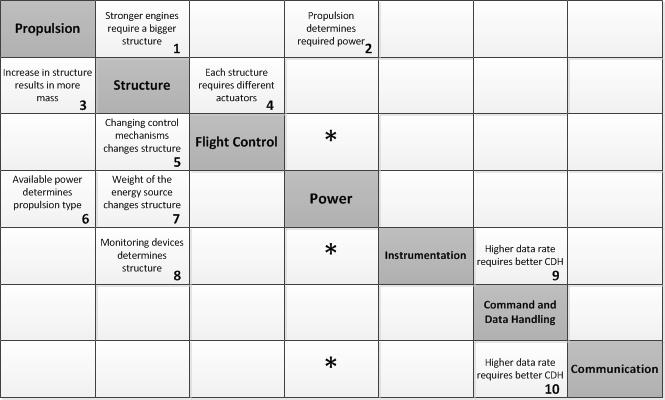
\includegraphics[width=\textwidth]{./Interfaces/Figures/N2Chart.jpg}
\caption{Design N2 Chart}
\label{fig:N2}
\end{figure}

\paragraph{Number 1} In order to integrate the propulsion subsystem in the system, structural support is needed. When for example the weight of the propulsion subsystem increases, more structural support is required. The structures subsystem design will also change when for example the location of the engines changes or the amount of thrust changes.

\paragraph{Number 2} The main power of the UAV is consumed by the propulsion subsystem. This means changing the propulsion engine will require a different energy source as either more or less power will be needed.

\paragraph{Number 3} Changing the structural subsystem of the UAV will also change the mass and external appearance of the system. More mass will lead to more thrust required for VTOL and hovering. A different external appearance will change the aerodynamics flows and hence the drag, requiring a different amount of thrust for horizontal flight. 

\paragraph{Number 4} The instability of the design is mainly determined by the structural subsystem. For example a conventional aircraft without tail-plane will require other means of control for pitching stability. Rotors could be used. After changing the structural design, the stability of the UAV thus has to be analysed again and the necessary actuators, as ailerons, or rotors need to be added. 

\paragraph{Number 5} By changing the control mechanisms of the UAV, different structural components need to be used in order to carry the loads induced by the new control surfaces.


\paragraph{Number 6} When for example due to a constraint the amount of power is limited, a different (more efficient) propulsion system has to be selected in order to be able to provide the required thrust. 


\paragraph{Number 7} A change in the power subsystem, like for example a different type of battery will result in a different take-off mass. This will have an effect on the structure, not only due to the weight, but also due to the volume the power subsystem might take up or the location of the battery. 


\paragraph{Number 8} A change in instrumentation will mean the volume occupied by this subsystem will change. The weight will also change but the volume change will have a greater effect on the structure.


\paragraph{Number 9} The data handling needs to process all the information coming from the instrumentation subsystem, this means that the size of the data handling subsystem needs to be sized for the amount of data coming from the instruments.

\paragraph{Number 10} This relation resembles Number 9, when there is a lot of communication, there is more data to be handled, this will increase the size of the command and data handling subsystem.

\paragraph{*} As it is the case with the propulsion subsystem, the flight control, instrumentation and communication subsystem all determine the amount of power required. However, compared to the power required by the propulsion subsystem, these subsystem use a negligible amount of power. The power subsystem is mainly driven by the required propulsion power requirements. 

\section{Function N2 Chart}
\label{sec:n2func}
Besides the subsystem interface N2 chart, there is also the functional N2 chart. This chart shows for a number of subsystems the functional relationships during operating phase. \autoref{fig:opsN2} shows the function N2 chart of the UAS. Two clear blocks can be distinguished; one related to the ground station and one related to the actual UAV in the operational phase. In can be seen that the connecting element between the two blocks is the 'Command and Data Handling block'.

\begin{figure}[htb]
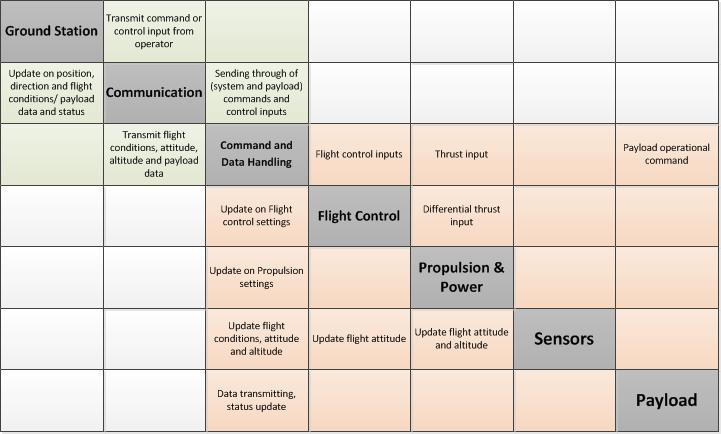
\includegraphics[width=\textwidth]{./Interfaces/Figures/N2ops.jpg}
\caption{Functional N2 Chart}
\label{fig:opsN2}
\end{figure}

The ground station of the UAS, where operator inputs originate from, is connected with the UAV by means of a communication subsystem block. By means of this communication block the the ground station receives status updates of the payload and the UAV (i.e. flight conditions and attitude) and the UAV receives commands or control inputs. All incoming commands are processed by the Command and Data Handling block. All data from the UAV subsystems feed to this block as well. That makes the Command and Data Handling the connecting element between the ground station and the UAV.

Flight Control is the subsystem that proves flight control to the UAV; it enables the UAV to have the required attitude and direction, furthermore it provides stability. This is done either by control surfaces or by means of differential thrust (depending on the flight phase the UAV is in).

The Sensors block is the UAV's connection with its environment; together with the data handling, it enables the UAV to operate autonomously.





    \chapter{Sustainable Development}
\label{ch:sustaindev}
\setlength{\parindent}{15pt}

Cradle to Cradle tool has been discarded due to the fact that certain materials such as carbon fibre composites and electronic components cannot be recycled to a raw material phase completely. Thus, only Life Cycle Assessment (LCA) is considered from this point of the project. The technical framework for LCA can be seen in \autoref{fig:lcatriangle}. It starts with the central block, 'Goal and Scope', then can flow into Impact Assessment and Inventory Analysis \cite{lca}.

\begin{figure}[H]
    \centering
    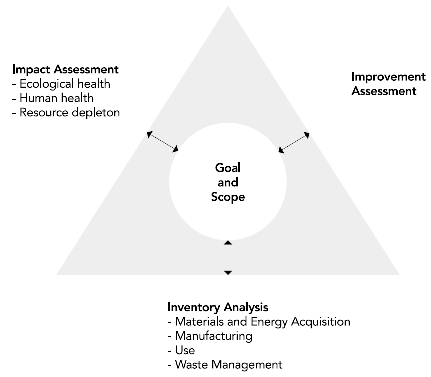
\includegraphics[width=0.6\textwidth]{SustainableDev/Figures/LCAtriangle.pdf}
    \caption{Technical Framework for Life Cycle Assessment}
    \label{fig:lcatriangle}
\end{figure}


\section{Goal and Scope}
The goal and scope definitions need to be determined as a first process of a LCA. The following paragraphs elaborate on details of each aspect of the first process. 

\paragraph{Goal} A mission need statement (MNS) can be used to define the goal. The MNS states, 'Carry out both supervised and autonomous monitoring and transport missions, comprising vertical take-off and landing, and high-velocity in horizontal flight.'

\paragraph{Scope} Since the project will stretch to planning of production of the UAV, it is important to define detailed assessment methods to be used. In order to define the assessment methods, a system to be studied and system boundaries need to be determined. Functions of the system have been identified based on a functional breakdown structure in the baseline report\cite{baseline}. 

\begin{itemize}
    \item Perform air transport
    \item Perform various missions
    \item Perform missions under various conditions
\end{itemize}

\paragraph{Functional Unit}
A main purpose for a functional unit is to set a normalised basis of comparison. For a consistent analysis, it is decided that further quantitative comparison will have a normalised scale from 0 to 100.

\paragraph{System Boundaries}
System boundaries are defined based on requirements, which can be found in \autoref{ch:requ}.

\paragraph{Data Quality}
Data quality in LCA is reflected in the final LCA. At this point of the stage, it is not possible to come up with a consistent and traceable data quality, such as time-related coverage, geographical coverage and technological coverage\cite{lca}. It will be established in the next phase of the project. 

\paragraph{Critical Review Process}
Critical review process is not applicable to this project, since the process is mainly for certification of a system or product and publication of the project in terms of environmental standards.

\section{Inventory Analysis}
Inventory analysis is carried out after defining goal and scope definition. A robust and qualitative inventory analysis can be carried out, as sustainability analysis is done and a production plan for the final concept is constructed.

\subsection{Materials and Energy Acquisition}
Relevant quantitative data has to be collected, but it is not possible at this point of the project, as parts of the UAV are not specified down to depth of types of materials and dimensions. Inputs and outputs of a product system need to be identified in order to identify materials and energy acquisition. In order to construct a UAV, raw materials are taken and processed into parts. Inputs during this stage are raw materials, energy spent to process raw materials into parts, labour and machines used for processing and production, while outputs can be parts or products. According to \autoref{ch:sustain}, chosen materials are EPP (polypropylene), aluminium and carbon fibre (polymer variants). Transforming raw materials into parts can be done by using thermal and kinetic energy, based on a type of manufacturing and process methods. The thermal and kinetic energy can be obtained by operating relevant machines using fossil fuel and stored electricity from a power plant.

\subsection{Manufacturing and Use}
Since manufacturing methods are not defined at this point of the project, it shall not be discussed. In the next phase of the project, the manufacturing aspect of the UAV will be defined and developed. For the sustainable development, the use phase will be focused on pre-flight preparation and post-flight maintenance. \autoref{fig:opslogsdig} in \autoref{sec:ol} shows relevant tasks for the pre-flight preparation and post-flight maintenance. For example, a truck is chosen for transporting staff members and equipment. Instead of using a standard cargo truck, vehicles with higher fuel efficiency can be used in order to decrease an environmental impact of the transport mean. For maintenance and overhaul, engineers and mechanics can ensure that damaged parts are properly repaired to minimise the number of discarded parts.

\subsection{Waste Management}
Waste management depends on the type of UAV parts. Analysed concepts in \autoref{ch:sustain} have varying materials, thus waste management per material differs. For instance, aluminium and polypropylene parts can be disassembled and directly recycled into new parts through a recycle process, but carbon fibre parts cannot be recycled into new parts for UAVs. A recycling process of carbon fibres normally includes chopping or milling\footnote{\url{http://www.compositesworld.com/articles/carbon-fiber-life-beyond-the-landfill}, Accessed 24-05-2017}, which lowers mechanical properties of resulting carbon fibres. Thus, it is assumed that heavily damaged and discarded carbon fibre parts for the UAV can be considered as non-recyclable waste. Batteries for UAVs will last many cycles before they have to be disposed. Lithium-ion batteries are commonly used for UAVs, and they can be disposed and recycled with certain emission of toxic elements.

\section{Impact Analysis}
After the inventory analysis is complete, impact analysis can be carried out. There are several impact categories to be considered as following: abiotic resources, biotic resources, land use, global warming, stratospheric ozone depletion, ecotoxicological impacts, human toxicological impacts, photochemical oxidant formation, acidification, eutrophicaition, work environment. Detailed analysis on each impact category will be carried out in the next phase of the project, as the current inventory analysis is qualitative. The impact analysis is consist of 'Ecological and Human Health' and 'Resource Depletion', and each sub categories will be investigated once materials and parameters of the UAV are finalised.

\section{Interpretation}
Interpretation is the last phase in LCA and includes identification of significant environmental issues, evaluation and conclusions and recommendations\cite{lca}. Once again, they will be assessed in depth when detailed development is complete.  

    \chapter{Technical Risk Assessment}
\label{ch:tech_risk_asse}

In the baseline report \cite{baseline}, a technical risk assessment was made based on all requirements. Since the properties of the concepts have been assessed, it has already become more clear what requirements are driving, key or killing (\autoref{ch:requ}). First, all risks that will not require more detailed assessing will be identified; more information on the risks on these requirements can be found in the baseline report \cite{baseline}. Then, a discussion on the risks that were deemed relevant can be seen in \autoref{sec:asse_requ}.

\section{Risk Identification}
\label{sec:risk_iden}
In this section, it will be determined what requirements pose technical risks for some specific concepts. Therefore, the requirements, as can be seen in \autoref{ch:requ}, have been examined. The requirements that were not taken on in the further technical risk assessment can be found below, along with the reasoning behind it. After that, the requirements that actually were taken on in this technical risk analysis can be found in \autoref{sec:asse_requ}.

\subsection{General groups of requirements} First, it was determined what groups of requirements would not have to be included in this technical risk assessment. These are discussed here.

\paragraph{Non-critical requirements}
All requirements labelled with an asterisk will not be assessed per concept. This is because these are non-critical requirements and therefore no added value is obtained from assessing the risk of not meeting these requirements per concept.

\paragraph{Third level requirements}
All requirements have been divided into different categories, and numbered in levels. Each requirement that is third level (like 1.1.1) or lower, will not be taken on into the technical risk analysis. This is done because these go into detail too deep for the risk assessment.

\paragraph{Legislation}
Requirements pertaining to legislation will not be assessed per concept. This is because these requirements, if met for one concept can easily be met for all concepts. Special risk assessment on a per concept basis is therefore not required.

\paragraph{Resource}
The only resource requirement, SYS-R-1, which states that the project and design shall not be performed by more than 10 team members is both a requirement which is not worth assessing the risk of not meeting as well as poses a risk which cannot be mitigated.

\paragraph{Vehicle systems}
The vehicle systems requirements (VS) discuss the communication systems and the propulsion system. The communication systems are related to the ground system and the other vehicles the UAV will have to communicate with -- both are the same for each concept. Also, in each concept electrical propulsion was chosen. Because of this, there will be no differences in technical risk related to vehicle systems requirements, making inclusion unnecessary.


\subsection{Specific requirements}
The risk of not meeting the following requirements which are not a part of the aforementioned requirement groups will also not be assessed per concept. 

\paragraph{Cost}

\begin{description}
    \item[SYS-C-2] Since the exact parts that will be used in each UAV have not been determined, the maintenance support service cost can not be estimated yet. Also, the ground station is the same for each concept, so there will be no differences there.
\end{description}


\paragraph{Environmental}

\begin{description}
    \item[SYS-ENV-2.2] This requirement concerns environmental influences of the UAV. Since electrical propulsion is used in each concept, this requirement will be met for each concept.
    \item[SYS-ENV-2.5] The risk associated with not meeting this requirement can be considered to be of the same magnitude for all concepts and depends on the production plan. The production plan can be manipulated such that it does meet this requirement for each concept.
\end{description}


\paragraph{Physical}

\begin{description}
    \item[SYS-PH-1.2] The payload bay requirement is determined by the size of the fuselage. For each design, this requirement can easily be met since the fuselage will just be given the correct dimensions.
    \item[SYS-PH-2] This is a killer requirement, and none of the concepts are expected to be able to meet it. Because the result is then the same for each concept, this requirement has not been analysed.
    \item[SYS-PH-4.4] This requirement is not verifiable yet, and it is not possible to say anything about the concepts being able to do this or not. 
\end{description}


\paragraph{Operational}

\begin{description}
    \item[SYS-OP-2.1] The operational life of the concepts depends on the reliability of the components. Since no concept makes use of very unreliable parts, this only depends on the production process.
    \item[SYS-OP-2.2] As this requirement THIS ONE IS ABOUT RELIABILITY PLZ CHANGE
    \item[SYS-OP-2.7] Assessing the risk of not meeting this requirement for each concept gives no extra legitimacy to this technical risk assessment. This requirement can easily be met by installing the requisite night equipment.
\end{description}


\paragraph{Performance}

\begin{description}
    \item[SYS-PF-2.1, 2.2] Each concept has been designed for vertical take-off and landing (VTOL) and therefore this requirement will not be assessed in this risk analysis.
\end{description}
    




\section{Risk Assessment}
\label{sec:risk_asse}

The risk of not meeting the following requirements will be assessed as important insight into each concept is gained by doing so. For each concepts, the same requirements were used in the technical risk assessment.

Each requirement has been abbreviated: since each requirement was a system requirement, the 'SYS-' part of the requirements was taken out for clarity in the tables. In this section, the technical risk assessment of each concept will be presented in \Cref{tab:tail_risk_asse,tab:tand_risk_asse,tab:pran_box_risk_asse,tab:tilt_risk_asse,tab:wing_quad_risk_asse}. For every requirement, a score has been given for the likeliness of not meeting it (L) and the impact when it is not met (I). Each gets a grade between 1 (almost impossible or negligible) to 4 (very likely or critical). The risks are identified and quantified. These will be used in the next section for the risk maps.



\begin{table}[]
    \centering
    \caption{Tailsitter risk assessment}
    \label{tab:tail_risk_asse}
    \begin{tabularx}{\textwidth}{l L l l l}
        \toprule
        %\rowstyle{\bftext}
        Risk            & Impact and Likelihood explanation                & L     & I     & R
        \\ \midrule
        C-1             & Since other hybrid UAVs are priced higher than 30,000 Euros\footnotemark, the impact is not large when this requirement is not met. When cheaper materials are used, so no carbon fibre, it is also possible to meet this requirement.                                & 3      & 1     & 3
        \\ \hdashline
        PH-1.1          & The current sizing (\autoref{tab:wing_summ}) completely exceeds these dimensions. Measures were already explained in \autoref{ch:grou_hand}. & 4 & 1 & 4 
        \\ \hdashline
        PH-4.3          & Since the concept has only one location where propulsion is generated, the mission will fail when the propulsion system fails. & 2      & 3     & 6
        \\ \hdashline
        OP-1.1          & The payload loading and unloading mechanism is positioned at the bottom of the concept while it is hovering. This means the Tailsitter is only able to release its payload while hovering, but not while it is in horizontal flight. Because it makes use of a clicking mechanism, the chance of the payload getting stuck is very small.                                                             & 1      & 4     & 4                        
        \\ \hdashline
        PF-1.1          & The likelihood of not meeting this requirement is very low, since the conceptual design process was centred around some driving requirements, including this one.                                                           & 1     & 3     & 3
        \\ \hdashline
        PF-1.2          & In order to meet this requirement, the power required for maximum velocity for this concept is estimated at 2.8 kW. This means it is possible to fly at 200 km/h, but not for an hour.                                                        & 1     & 2     & 2
        \\ \hdashline
        PF-1.3          & Not meeting this requirement would mean that certain missions are not possible anymore. The probability of not meeting this requirement is influenced by the battery capacity.                                               & 2     & 2     & 4
        \\ \hdashline
        PF-1.4          & Based on \autoref{sec:endu_anal}, the Tailsitter concept might not meet the endurance requirement. However, when it has the power to fly at 200 km/h, it will also have enough power to fly for one hour. Not meeting this requirement influences the types of possible missions.                         & 2     & 3     & 6      
        \\ \hdashline
        PF-2.3          & The hovering is one of the most power-intensive flight stages, meaning this requirement depends on the battery capacity. Not being able to fulfil this requirement would limit the amount of different missions that can be performed.                                                                    & 2       & 3 & 6
        \\ \hdashline
        PF-2.4          & Climb speed is determined by the vertical propulsive forces. Having a too low climb speed would result into a lot of unnecessary energy loss, since horizontal flight is a lot more energy efficient.               & 2   & 4   & 8
        \\ \hdashline
        PF-3            & Since the Tailsitter only has some control surfaces in its tail and only one double propeller at its nose, controllability might be difficult, especially in vertical flight conditions like hovering.                  & 4     & 2 & 8
        \\ \hdashline
        PF-4            & In horizontal flight, the Tailsitter is expected to be stable for a limited range of centres of gravity. In vertical flight, the UAV will be stabilised using a stabiliser bar.             & 4 & 1 & 4
        \\ \bottomrule
    \end{tabularx}
\end{table}



\begin{table}[]
    \centering
    \caption{Tandem risk assessment}
    \label{tab:tand_risk_asse}
    \begin{tabularx}{\textwidth}{l L l l l}
        \toprule
        %\rowstyle{\bftext}
        Risk            & Impact and Likelihood explanation                & L     & I     & R
        \\ \midrule
        C-1             & Since other hybrid UAVs are priced higher than 30,000 Euros\footnotemark, the impact is not large when this requirement is not met. When cheaper materials are used, so no carbon fibre, it is also possible to meet this requirement.                                & 3      & 1     & 3
        \\ \hdashline
        PH-1.1          & In order to meet this requirement, it must be possible to split up the UAV in multiple parts. As can be seen in \autoref{sec:asse},%assembly section in ground handling
        the Tandem can be disassembled for transport. A disadvantage of this is the increase in structural weight.                 & 2     & 2     & 4
        \\ \hdashline
        PH-4.3          & Since the Tandem has four propellers that can provide thrust in vertical and horizontal direction, engine failure is not critical. Because it also has four wings, with control surfaces, redundancy is provided.                                         & 1         & 3     & 3
        \\ \hdashline
        OP-1.1          & The Tandem is loaded through the back of the fuselage, which means that dropping the payload during flight requires the UAV to turn its fuselage in the air. When it turns out this is not possible, it is allowed to change mounting location to the bottom of the UAV.       & 2 & 4 & 8
        \\ \hdashline
        PF-1.1          & Since the design was centred around, among others, the payload, this will be possible.          & 1 & 4 & 4
        \\ \hdashline
        PF-1.2          & In order to reach this requirement, the power required is estimated at 10.2 kW (\autoref{REFER} REFER TO THE TABLE). This would require a large battery.       & 2     & 1     & 2
        \\ \hdashline
        PF-1.3          & Not meeting this requirement would mean certain missions are not possible anymore.    & 2 & 3 & 6
        \\ \hdashline
        PF-1.4          & Not meeting this requirement would severely limit the amount of missions that can be performed.          & 2 & 4 & 8
        \\ \hdashline
        PF-2.3          & Not meeting this requirement would limit the type of missions that can be carried out. Since hovering is a very power consumption intensive flight phase, this depends on the installed battery.       & 3 & 4 & 12
        \\ \hdashline
        PF-2.4          & Since the vertical flight uses a lot of energy, having a lower climb speed will have a negative impact on the required power.              & 2 & 3  & 6
        \\ \hdashline
        PF-3            & Since the Tandem has four propellers in different locations, it can be controlled in vertical flight phases, even when its speed is zero. It also has enough control surfaces to fully control it during horizontal flight. The absence of the tail can be compensated through the propulsion system.      & 1        & 2 & 2
        \\ \hdashline
        PF-4            & The Tandem is expected to be stable during horizontal flight. Like a regular quadcopter, it is not stable during vertical flight but is controlled using the propellers.     & 4 & 1 & 4
        \\ \bottomrule
    \end{tabularx}
\end{table}




\begin{table}[]
    \centering
    \caption{Prandtl Box risk assessment}
    \label{tab:pran_box_risk_asse}
    \begin{tabularx}{\textwidth}{l L l l l}
        \toprule
        %\rowstyle{\bftext}
        Risk            & Impact and Likelihood explanation                & L     & I     & R
        \\ \midrule
        C-1             & If this requirement is not met, the effect on the project is not catastrophic as the estimated cost is expected to be between 30,000 and 60,000 Euros \footnotemark.                                                                     & 1     & 3     & 3
        \\ \hdashline
        PH-1.1          & The span of each wing in this concept is approximately 2 m and would therefore require dismantling in order to meet this requirement. Because of the Prandtl box wing concept even further divides will be required to fit everything in the prescribed volume. This will result in weight increases.    & 2 & 3 & 6  
        \\ \hdashline
        PH-4.3          & If this requirement was not to be met the risk of the UAV not being able to complete the required mission is high. For this concept the likelihood of not meeting this requirement is low.                                                                                 & 1      & 3     & 3 
        \\ \hdashline
        OP-1.1          & If this requirement is not met the possible missions are limited to surveillance type missions. For this concept this is not an issue because of the layout of the fuselage.   & 1 & 3 & 3
        \\ \hdashline
        PF-1.1          & The likelihood of not meeting this requirement is low as the design is centred around the payload. The missions will be affected if this requirement is not met.                                                                                                                 & 1 & 2 & 2
        \\ \hdashline
        PF-1.2          & If this requirement is not met time sensitive missions will be affected. The power required for this concept to meet this requirement is 9.0 kW which split over four motors is manageable, however this is a lot of power to be drawn from the batteries.  & 2 & 3 & 6
        \\ \hdashline
        PF-1.3          & If this requirement is not met the range sensitive missions might be affected. If \textbf{SYS-PF-1.3} is met for this concept then the likelihood of not meeting this requirement is negligible
                & 1 & 3 & 3
        \\ \hdashline
        PF-1.4          & If this requirement is not met many mapping and surveillance missions would no longer be possible. If \textbf{SYS-PF-1.3} is met for this concept then the likelihood of not meeting this requirement is negligible                                                          & 1 & 3 & 3
        \\ \hdashline
        PF-2.3          & Not meeting this requirement would greatly limit the types and number of missions that can be conducted. The power required for this concept to hover is 2.9 kW which can be easily attained.  & 1 & 4 & 4
        \\ \hdashline
        PF-2.4           & The power required to climb at 4 m/s is 3.76 kW and providing the climb phase is quite short the energy required is small in comparison the energy required for hovering. Not meeting this requirement is not that critical, a smaller climb rate would not drastically diminish the capabilities of the UAV.                                                                                                                             & 1 & 2 & 2 
        \\ \hdashline
        PF-3            & The controllability of this concept is very high and especially because of having 4 motors. The likelihood of not meeting this requirement is therefore quite low.    & 2 & 2 & 4
        \\ \hdashline        
        PF-4            & This concept can be designed such that it is longitudinally, directionally and laterally stable therefore the risk of not meeting this requirement is low.         & 1 & 3 & 3
        \\ \bottomrule
    \end{tabularx}
\end{table}



\begin{table}[]
    \centering
    \caption{Tiltrotor risk assessment}
    \label{tab:tilt_risk_asse}
    \begin{tabularx}{\textwidth}{l L l l l}
        \toprule
        %\rowstyle{\bftext}
        Risk            & Impact and Likelihood explanation                & L     & I     & R
        \\ \midrule
        C-1             & If this requirement is not met the effect on the project is not catastrophic as the estimated cost is expected to be between 30,000 and 60,000 Euros.                                                                                                                       & 1     & 3     & 3
        \\ \hdashline
        PH-1.1          & The span of The Tiltrotor is approximately 3.25 m which means that the only way this requirement can be satisfied is if the main wing can be dismantled into at least 2 pieces. Extra structural weight would be necessary to compensate for this segmentation.             & 2 & 3 & 6
        \\ \hdashline
        PH-4.3          & As this concept only has 2 rotors a complex redundancy system is required to meet this requirement. Not meeting this requirement can be critical to being able to fulfil the specified missions.                                                                            & 3 & 3 & 9
        \\ \hdashline
        OP-1.1          & Not meeting this requirement would limit the possible types of missions to surveillance and mapping. The likelihood of not meeting this requirement for this concept is small because of the fuselage configuration chosen.                                                     & 1 & 3 & 3 
        \\ \hdashline
        PF-1.1          & The likelihood of not meeting this requirement is low as the design is centred around the payload. The missions will be affected if this requirement is not met.                                                                                                                 & 1 & 2 & 2
        \\ \hdashline
        PF-1.2          & Not meeting this requirement would mean that missions where time is of the essence would be affected. The power required to meet this requirement for this concept is 8.0 kW which is a lot for both the motors (split over 2 motors) as well as power storage to manage.     & 3 & 3 & 9
        \\ \hdashline
        PF-1.3          & If this requirement is not met many mapping and surveillance missions would no longer be possible. If \textbf{SYS-PF-1.3} is met for this concept then the likelihood of not meeting this requirement is negligible                                                          & 2 & 3 & 6
        \\ \hdashline
        PF-1.4          & If this requirement is not met the types and duration of various surveillance and mapping missions will not be able to be carried out.                                                                                                                                          & 1 & 3 & 3
        \\ \hdashline
        PF-2.3          & The power required for this concept to hover is 5.06 kW and to pull this amount of power for a sustained 5 minutes requires quite a lot of stored energy. If this requirement is not met then many missions become impossible.                                                  & 2 & 3 & 6
        \\ \hdashline
        PF-2.4          & The power required to climb at 4 m/s is 6.51 kW and providing the climb phase is quite short the energy required is small in comparison the energy required for hovering. Not meeting this requirement is not that critical, a smaller climb rate would not drastically diminish the capabilities of the UAV.                                                                                                                             & 1 & 2 & 2 
        \\ \hdashline
        PF-3            & The controllability of this concept is quite bad in the vertical flight phases, however this can be compensated for by a robust control system.                                                                                                                                 & 2 & 3 & 6
        \\ \hdashline
        PF-4            & This concept can be designed such that it is longitudinally, directionally and laterally stable therefore the risk of not meeting this requirement is low.                                                                                                                      & 1 & 3 & 3
        \\ \bottomrule
    \end{tabularx}
\end{table}



\begin{table}[]
    \centering
    \caption{Winged Quadcopter risk assessment}
    \label{tab:wing_quad_risk_asse}
    \begin{tabularx}{\textwidth}{l L l l l}
        \toprule
        %\rowstyle{\bftext}
        Risk            & Impact and Likelihood explanation               & L     & I     & R
        \\ \midrule
        C-1             & If this requirement is not met the effect on the project is not catastrophic as the estimated cost is expected to be between 30,000 and 60,000 Euros.        & 1     & 3     & 3
        \\ \hdashline
        PH-1.1          & The span of The Winged Quadcopter is approximated at 3.20 m. If the wing can be dismantled into two parts then this poses no issue with regards this requirement. Extra weight might result from a more robust structure required.                           & 2     & 3     & 6
        \\ \hdashline
        PH-4.3          & If this requirement was not to be met the risk of the UAV not being able to complete the required mission is high. For this concept the likelihood of not meeting this requirement is low.                                                                                 & 1      & 3     & 3
        \\ \hdashline
        OP-1.1          & Not meeting this requirement would limit the UAV's missions to surveillance missions only. For this concept the likelihood of not being able to airdrop its payload is low because of the type of configuration.                                                       & 1     & 3     & 3
        \\ \hdashline
        PF-1.1          & The likelihood of not meeting this requirement is low as the design is centred around the payload. The missions will be affected if this requirement is not met.   & 1 & 2     & 2
        \\ \hdashline
        PF-1.2          & Not meeting this requirement would limit the types of missions that can be carried out. The power required for this concept to meet this requirement is 4.7 kW which is attainable. & 3 & 2 & 6
        \\ \hdashline
        PF-1.3          & Not meeting this requirement would mean that certain missions would be hindered. The likelihood of this happening is low based on reference craft of the same configuration. & 1 & 3 & 3        
        \\ \hdashline
        PF-1.4          & If this requirement is not met many mapping and surveillance missions would no longer be possible. If \textbf{SYS-PF-1.3} is met for this concept then the likelihood of not meeting this requirement is negligible.                                               & 2 & 3 & 6
        \\ \hdashline
        PF-2.3          & This requirement, if not met, means that the missions requiring this capability cannot be conducted. The power required to hover is 4.4 kW meaning that if \textbf{SYS-PF-1.3} is met for this concept then the likelihood of not meeting this requirement is negligible.   & 2 & 3 & 6
        \\ \hdashline
        PF-2.4          & The power required to climb at 4 m/s is 4.4 kW and providing the climb phase is quite short the energy required is small in comparison the energy required for hovering. Not meeting this requirement is not that critical, a smaller climb rate would not drastically diminish the capabilities of the UAV.                                                                               & 1 & 2 & 2 
        \\ \hdashline
        PF-3            & The controllability of this concept is very high and especially because of being a quadcopter. The likelihood of not meeting this requirement is therefore quite low.    & 2 & 2 & 4
        \\ \hdashline        
        PF-4            & This concept can be designed such that it is longitudinally, directionally and laterally stable therefore the risk of not meeting this requirement is low.         & 1 & 3 & 3
        \\ \bottomrule  
    \end{tabularx}
\end{table}











\section{Mapping and Mitigation of Risks}
\label{sec:mapp_miti_risk}
Based on \autoref{sec:risk_asse}, the risks are presented in risk maps, where the actual risk is visualised. Everything that is in the green part of the maps (bottom left corner) is not problematic. All requirements that are in the yellow or red part, however, must be mitigated. The top right corner, the red part, is the place where the biggest threats can be found.






\begin{table}[H]
    \centering
    \caption{Risk map of the Tailsitter}
    \label{tab:risk_map_tail}
    \begin{tabular}{p{2.5cm}p{2.5cm}p{2.5cm}p{2.5cm}p{2.5cm}}
    \toprule
                    & (Almost) impossible           & Improbable                    & Probable                          & Very likely
    \\ \midrule
    Catastrophic    &\cellcolor[HTML]{d9ead3} OP-1.1      &\cellcolor[HTML]{fff2cc}  PF-2.4       &\cellcolor[HTML]{f4cccc}           &\cellcolor[HTML]{f4cccc}
    \\ \hdashline
    Critical        &\cellcolor[HTML]{d9ead3} PF-1.1      &\cellcolor[HTML]{fff2cc} PH-4.3, PF-1.4, PF-2.3      &\cellcolor[HTML]{fff2cc}           &\cellcolor[HTML]{f4cccc}
    \\ \hdashline
    Marginal        &\cellcolor[HTML]{d9ead3} PF-1.2      &\cellcolor[HTML]{d9ead3} PF-1.3      &\cellcolor[HTML]{fff2cc}           &\cellcolor[HTML]{fff2cc}  PF-3
    \\ \hdashline
    Negligible      &\cellcolor[HTML]{d9ead3}       &\cellcolor[HTML]{d9ead3}       &\cellcolor[HTML]{d9ead3}  C-1         &\cellcolor[HTML]{d9ead3} PH-1.1,  PF-4
    \\ \bottomrule
    \end{tabular}
\end{table}


\begin{table}[H]
    \centering
    \caption{Risk map of Tandem}
    \label{tab:risk_map_tand}
    \begin{tabular}{p{2.5cm}p{2.5cm}p{2.5cm}p{2.5cm}p{2.5cm}}
    \toprule
                    & (Almost) impossible           & Improbable                    & Probable                          & Very likely
    \\ \midrule
    Catastrophic    &\cellcolor[HTML]{d9ead3} PF-1.1       &\cellcolor[HTML]{fff2cc} OP-1.1,  PF-1.4      &\cellcolor[HTML]{f4cccc} PF-2.3          &\cellcolor[HTML]{f4cccc}
    \\ \hdashline
    Critical        &\cellcolor[HTML]{d9ead3} PH-4.3      &\cellcolor[HTML]{fff2cc} PF-1.3, PF-2.4      &\cellcolor[HTML]{fff2cc}           &\cellcolor[HTML]{f4cccc}
    \\ \hdashline
    Marginal        &\cellcolor[HTML]{d9ead3} PF-3      &\cellcolor[HTML]{d9ead3}  PH-1.1     &\cellcolor[HTML]{fff2cc}           &\cellcolor[HTML]{fff2cc}
    \\ \hdashline
    Negligible      &\cellcolor[HTML]{d9ead3}       &\cellcolor[HTML]{d9ead3}  PF-1.2     &\cellcolor[HTML]{d9ead3} C-1          &\cellcolor[HTML]{d9ead3} PF-4
    \\ \bottomrule
    \end{tabular}
\end{table}



\begin{table}[H]
    \centering
    \caption{Risk map of Prandtl Box}
    \label{tab:risk_map_pran_box}
    \begin{tabular}{p{2.5cm}p{2.5cm}p{2.5cm}p{2.5cm}p{2.5cm}}
    \toprule
                    & (Almost) impossible                                               & Improbable                            & Probable                          & Very likely
    \\ \midrule
    Catastrophic    &\cellcolor[HTML]{d9ead3}   PF-2.3                                        &\cellcolor[HTML]{fff2cc}               &\cellcolor[HTML]{f4cccc}           &\cellcolor[HTML]{f4cccc} 
    \\ \hdashline
    Critical        &\cellcolor[HTML]{d9ead3} PH-1.1, PH-4.3, OP-1.1, PF-1.3, PF-1.4, PF-4   &\cellcolor[HTML]{fff2cc} PH-1.1, PF-1.2 &\cellcolor[HTML]{fff2cc}           &\cellcolor[HTML]{f4cccc}
    \\ \hdashline
    Marginal        &\cellcolor[HTML]{d9ead3}  PF-1.1, PF-2.4                            &\cellcolor[HTML]{d9ead3}  PF-3         &\cellcolor[HTML]{fff2cc}           &\cellcolor[HTML]{fff2cc}
    \\ \hdashline
    Negligible      &\cellcolor[HTML]{d9ead3}                                           &\cellcolor[HTML]{d9ead3}               &\cellcolor[HTML]{d9ead3}           &\cellcolor[HTML]{d9ead3}
    \\ \bottomrule
    \end{tabular}
\end{table}


\begin{table}[H]
    \centering
    \caption{Risk map of Tiltrotor}
    \label{tab:risk_map_tilt}
    \begin{tabular}{p{2.5cm}p{2.5cm}p{2.5cm}p{2.5cm}p{2.5cm}}
    \toprule
                    & (Almost) impossible           & Improbable                    & Probable                          & Very likely
    \\ \midrule
    Catastrophic    &\cellcolor[HTML]{d9ead3}       &\cellcolor[HTML]{fff2cc}       &\cellcolor[HTML]{f4cccc}           &\cellcolor[HTML]{f4cccc}
    \\ \hdashline
    Critical        &\cellcolor[HTML]{d9ead3} C-1, OP-1.1, PF-1.4, PF-4       &\cellcolor[HTML]{fff2cc} PH-1.1, PF-1.3, PF-2.3, PF-3      &\cellcolor[HTML]{fff2cc}   PH-4.3, PF-1.2         &\cellcolor[HTML]{f4cccc}
    \\ \hdashline
    Marginal        &\cellcolor[HTML]{d9ead3} PF-1.1, PF-2.4      &\cellcolor[HTML]{d9ead3}       &\cellcolor[HTML]{fff2cc}           &\cellcolor[HTML]{fff2cc}
    \\ \hdashline
    Negligible      &\cellcolor[HTML]{d9ead3}       &\cellcolor[HTML]{d9ead3}       &\cellcolor[HTML]{d9ead3}           &\cellcolor[HTML]{d9ead3}
    \\ \bottomrule
    \end{tabular}
\end{table}


\begin{table}[H]
    \centering
    \caption{Risk map of Winged Quadcopter}
    \label{tab:risk_map_wing_quad}
    \begin{tabular}{p{2.5cm}p{2.5cm}p{2.5cm}p{2.5cm}p{2.5cm}}
    \toprule
                    & (Almost) impossible                                       & Improbable                                    & Probable                          & Very likely
    \\ \midrule
    Catastrophic    &\cellcolor[HTML]{d9ead3}                                   &\cellcolor[HTML]{fff2cc}                       &\cellcolor[HTML]{f4cccc}           &\cellcolor[HTML]{f4cccc}
    \\ \hdashline
    Critical        &\cellcolor[HTML]{d9ead3} C-1, PH-4.3, OP-1.1, PF-1.3, PF-4     &\cellcolor[HTML]{fff2cc} PH-1.1, PF-1.4, PF-2.3  &\cellcolor[HTML]{fff2cc}           &\cellcolor[HTML]{f4cccc}
    \\ \hdashline
    Marginal        &\cellcolor[HTML]{d9ead3} PF-1.1, PF-2.4                     &\cellcolor[HTML]{d9ead3}  PF-3                 &\cellcolor[HTML]{fff2cc} PF-1.2    &\cellcolor[HTML]{fff2cc}
    \\ \hdashline
    Negligible      &\cellcolor[HTML]{d9ead3}                                   &\cellcolor[HTML]{d9ead3}                       &\cellcolor[HTML]{d9ead3}           &\cellcolor[HTML]{d9ead3}
    \\ \bottomrule
    \end{tabular}
\end{table}










\section{Risk Mitigation}

In this section, the mitigation measures will be described for each concept. In \Cref{tab:miti_tail,tab:miti_pran_box,tab:miti_tand,tab:miti_tilt,tab:miti_wing_quad} the measures are presented per concept. The old risk, R, is presented along with the mitigated risk, M, that arises from the new likelihood of occurrence (L) and impact (I).

\begin{table}[H]
    \centering
    \caption{Mitigation measures for problematic risks of the Tailsitter}
    \label{tab:miti_tail}
    \begin{tabularx}{\textwidth}{l L *{4}{c}}
    \toprule
    Risk            & Impact and Likelihood explanation             &       L   & I & M & R           
    \\ \midrule
    PH-4.3          & Make sure to install a very reliable propeller.  &    1   & 3 & 3 & 6
    \\ \hdashline
    PF-1.4          & Decide that endurance is more important than the mass and cost, and install a battery large enough to meet the requirement.                         & 1 & 3 & 3 & 6
    \\ \hdashline
    PF-2.3          & Install powerful propellers.                       &   1   & 3 & 3 & 6                           
    \\ \hdashline
    PF-2.4          & Install powerful propellers.                       &   1   & 4 & 4 & 8
    \\ \hdashline
    PF-3            & Enable extra controllability using the double propeller.   & 2 & 2 & 4 & 8
    \\ \bottomrule
    \end{tabularx}
\end{table}



\begin{table}[H]
    \centering
    \caption{Mitigation measures for problematic risks of the Tandem}
    \label{tab:miti_tand}
    \begin{tabularx}{\textwidth}{l L *{4}{c}}
    \toprule
    Risk            & Impact and Likelihood explanation                                     & L & I & M & R
    \\ \midrule
    OP-1.1          & Change mounting location.                                             & 1 & 4 & 4 & 8
    \\ \hdashline
    PF-1.3          & Install powerful propellers.                                      &   1   & 3 & 3 & 6 
    \\ \hdashline
    PF-1.4          & Install powerful propellers.                                      &   1   & 4 & 4 & 8 
    \\ \hdashline
    PF-2.3 & Install large battery.                                            &   1   & 4 & 4 & 8 
    \\ \hdashline
    PF-2.4          & Install powerful propellers.                                      &   1   & 3 & 3 & 6 
    \\ \bottomrule
    \end{tabularx}
\end{table}


\begin{table}[H]
    \centering
    \caption{Mitigation measures for problematic risks of the Prandtl Box}
    \label{tab:miti_pran_box}
    \begin{tabularx}{\textwidth}{l L *{4}{c}}
    \toprule
    Risk            & Impact and Likelihood explanation                             & L & I & M & R
    \\ \midrule
    PH-1.1          & Find an efficient way to be able to divide the structure in multiple parts without adding excessive extra structural weight.                             & 2 & 2 & 4 & 6
    \\ \hdashline
    PF-1.2          & Install a battery and propulsion system that can provide enough power.       & 1 & 3 & 3 & 6
    \\ \bottomrule
    \end{tabularx}
\end{table}

\iffalse
\begin{table}
    \centering
    \caption{Mitigation measures for problematic risks of the Tiltrotor}
    \label{tab:miti_tilt}
    \begin{tabularx}{\textwidth}{l L *{4}{c} }
    \toprule
    Risk            & Impact and Likelihood explanation                             & L & I & M & R
    \\ \midrule
    PH-1.1          & Devise an efficient way of dividing the structure such that it fits into the prescribed volume.     & 1 & 3 & 3 & 6
    \\ \hdashline
    PH-4.3          & Design redundancy system allowing an one rotor to be powered by the other motor in the event that it fails. & 2 & 2 & 4 & 9
    \\ \hdashline
    PF-1.2          & Install a battery and propulsion system that can store and provide the requisite amount energy.              & 2 & 3 & 6 & 9
    \\ \hdashline
    PF-1.3          & Install a battery capable of providing the required energy.                                                 & 1 & 3 & 3 & 6
    \\ \hdashline
    PF-2.3          & Install a battery and propulsion system that can store and provide the requisite amount energy.              & 1 & 3 & 3 & 6
    \\ \hdashline
    PF-3            & Spend considerable resources developping a control system capable of boosting controllability               & 1 & 3 & 3 & 6
    \\ \bottomrule
    \end{tabularx}
\end{table}




\begin{table}
    \centering
    \caption{Mitigation measures for problematic risks of the Winged Quadcopter}
    \label{tab:miti_wing_quad}
    \begin{tabularx}{\textwidth}{l L *{4}{c} }
    \toprule
    Risk            & Impact and Likelihood explanation
    \\ \midrule
    PH-1.1          & Devise an efficient way of dividing the structure such that it fits into the prescribed volume.     & 1 & 3 & 3 & 6
    \\ \hdashline
    PF-1.2          & Install a battery and propulsion system that can store and provide the requisite amount of energy.              & 1 & 3 & 3 & 6
    \\ \hdashline
    PF-1.4          & Install a battery and propulsion system that can store and provide the requisite amount of energy.              & 1 & 3 & 3 & 6
    \\ \hdashline
    PF-2.3          & Install a battery that can provide the required amount of energy.              & 1 & 3 & 3 & 6
    \\ \bottomrule
    \end{tabularx}
\end{table}

\fi

    \chapter{Production Plan}
\label{ch:prod_plan}

In case the finalised concept will be produced by series production, a production plan will come in handy to show the required activities to build the aircraft. The production plan shows, in general lines, which steps need to be taken into building the aircraft, and which steps can be done concurrently. \autoref{fig:pp_top} shows the production plan for The Winged Quadcopter.

\begin{figure}[H]
    \centering
    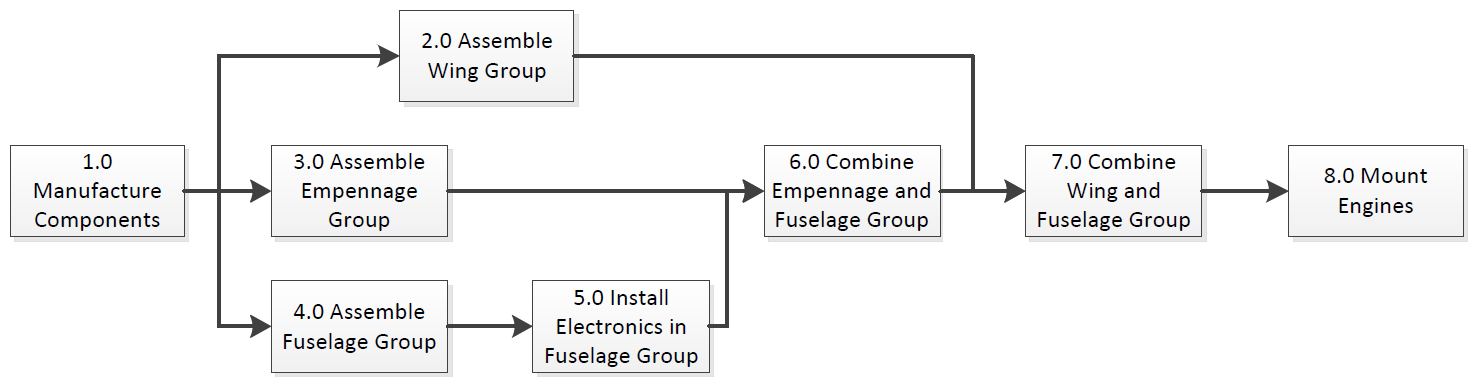
\includegraphics[width=\textwidth]{ProductionPlan/Figures/pp_top}
    \caption{Top Level Production Flow Diagram}
    \label{fig:pp_top}
\end{figure}

Looking at the top level, all of the required parts are manufactured first. Next, the three main groups of the aircraft can be constructed simultaneously, namely the fuselage, empennage and wing. Once these are constructed the assembly can begin, starting with the fuselage and the empennage, followed by the wing. This order has been chosen because the wings will complicate the process by taking up a lot of space. Tthe engines are mounted last in order to minimise the risk of damaging them or the UAV during production.

Each assembly stage presented in the top level is shown in detail below, starting with the wing assembly, \autoref{fig:pp_2}. Here, the wing structure is constructed by first creating a base for all other components to be fixed to. The exact type of base will be determined at a further development stage, depending on the materials used. Next, parts such as control surfaces or engine mounts are constructed and mounted onto the base. Finally, an outer layer is added for various purposes such as strength or protection. Again, this will depend on the materials chosen.

\begin{figure}[H]
    \centering
    \includegraphics[width=\textwidth]{ProductionPlan/Figures/pp_2}
    \caption{Wing Assembly Flow Diagram}
    \label{fig:pp_2}
\end{figure}

The detailed empennage assembly is shown in \autoref{fig:pp_3}. This production stage comprises three parallel processes, namely the construction of the vertical and horizontal stabilisers, as well as of the empennage base. These are then assembled together, after which the actuators are mounted onto the base and connected to the control surfaces. The stage ends with the addition of an outer layer to the entire empennage.

\begin{figure}[H]
    \centering
    \includegraphics[width=\textwidth]{ProductionPlan/Figures/pp_3}
    \caption{Empennage Assembly Flow Diagram}
    \label{fig:pp_3}
\end{figure}

The construction of the fuselage is split into two stages, namely the structural assembly (\autoref{fig:pp_4}) and the installation of the electronics in the fuselage (\autoref{fig:pp_5}). The first stage consists of constructing the fuselage base and payload bay in parallel, and then assembling them together. The undercarriage is mounted afterwards making it easier to assemble the payload bay beforehand. With the undercarriage installed, from this stage on the UAV will not require any additional structural supports during production. Finally, the engine mounts are attached to the fuselage. 

\begin{figure}[H]
    \centering
    \includegraphics[width=0.8\textwidth]{ProductionPlan/Figures/pp_4}
    \caption{Fuselage Structure Assembly Flow Diagram}
    \label{fig:pp_4}
\end{figure}

The second stage consists of installing the cabling and the control computer first. The control computer will make it possible to test all the electrical components on the UAV, such as the actuators or motors. Performing these tests immediately after the installation of each electrical component will make it easier to fix or replace them if needed. Next the sensors and communication system are mounted on the fuselage.

\begin{figure}[H]
    \centering
    \includegraphics[width=\textwidth]{ProductionPlan/Figures/pp_5}
    \caption{Fuselage Electronics Assembly Flow Diagram}
    \label{fig:pp_5}
\end{figure}

Next, the empennage is assembled with the fuselage first (\autoref{fig:pp_6}), followed by the assembly of the fuselage with the wings(\autoref{fig:pp_7}). Both these processes consist of joining the structures, connecting the cable harnesses, and testing all the connections and actuators. The only exception is that during the fuselage-empennage stage, an outer layer is finally added to the fuselage structure. Delaying this step makes it easier to connect the structures and install all electronic components.

\begin{figure}[H]
    \centering
    \includegraphics[width=0.9\textwidth]{ProductionPlan/Figures/pp_6}
    \caption{Fuselage and Empennage Joining Flow Diagram}
    \label{fig:pp_6}
\end{figure}

\begin{figure}[H]
    \centering
    \includegraphics[width=0.8\textwidth]{ProductionPlan/Figures/pp_7}
    \caption{Fuselage and Wing Joining Flow Diagram}
    \label{fig:pp_7}
\end{figure}

The last step (\autoref{fig:pp_8}) involves mounting the engines to the wings and fuselage. It is assumed that the engines will be heavy, hence attaching them last will make it easier to handle the product during the preceding production stages. In addition, there will be a lesser risk of damaging the UAV or the engines themselves during improper handling.

\begin{figure}[H]
    \centering
    \includegraphics[width=0.8\textwidth]{ProductionPlan/Figures/pp_8}
    \caption{Engine Mounting Flow Diagram}
    \label{fig:pp_8}
\end{figure}

%Constructing the wings will be straightforward. The empennage however has some concurrent construction going on, the assembly of the three pieces must be done in a specific order because the empennage is a T-tail. The order has been chosen to first assemble the base and the vertical tail, followed by the horizontal tail. WRITE LATER WHEN WE KNOW MORE ABOUT G
    \chapter{Operations \& Logistics}
\label{sec:ol}
%introduction
In this chapter the operational and logistical aspects of the design will be evaluated provisionally. It is not part of the trade-off concept since all concepts share the same procedures and infrastructure, but is intended to serve as preparation for the detailed design phase. A flow diagram describing support facilities, equipment and activities is included, as well as considerations on the mission operation itself.  

\section{Ground operations and logistics}

\begin{figure}[htb]
    \centering
    \includegraphics[width=1.05\textwidth]{Operations/Figures/operations_logistics.pdf}
    \caption{Operations \& logistics flow diagram}
    \label{fig:opslogsdig}
\end{figure}

\autoref{fig:opslogsdig} shows the the operations and logistics flow diagram for what this group expects to be typical operating conditions. It is assumed that the UAV operator has a main facility, from which the UAV, staff and mission relevant equipment are transported to a mission base at which flight operations take place. Naturally, variations to this scheme are possible, e.g. a parcel company may exclusively operate from its main facility, or long-range missions require a turn-around at a remote location, but for the sake of brevity only the most general case is presented.
The starting and end points of each mission are the so-called 'headquarters', the place where maintenance and storage takes place. Based on customer input a mission plan is set up, which determines the kind of resources that are required. Next to one or more UAVs, this includes staff on site, equipment such as the ground station, spare parts, additional batteries and a transport vehicle. Once the preparation is done, everything is loaded into a vehicle and transported to the location where the UAV is intended to take off and land. On site, the equipment needs to be unloaded and the UAV assembled into its operational form. A charged battery is then loaded, followed by the payload, which can also consist of another set of batteries. The system is switched on, the mission relevant data is uploaded to the on-board computer and an automated instrument calibration and readiness check performed. The UAV is now ready to fly and carry out its mission. After its return, the system is switched off for safety reasons, visually inspected and stripped off its batteries. The next steps depend on the kind of mission in question. If another flight is scheduled, the payload can be replaced and minor repairs taken out, e.g. replacing a damaged propeller blade. Once the battery is recharged or replaced by a full one, a new flight cycle can start. In case the mission does not comprise a turn-around or substantial damage was detected, the digital flight log is updated and the UAV disassembled. After loading all equipment the transport back to the headquarter takes place, where scheduled maintenance and all levels of repairs are carried out. Once the work is documented and approved, the equipment is stored and ready for the next mission. 


\section{Flight operations}

The amount of human interaction in flight operations varies depending on future regulations on what level of autonomy will be allowed. Current regulations only allow for operations within visual line of sight, which means that a pilot has to be able to see the UAV at all times and take control from automated systems immediately. While this is acceptable for certain mission profiles, the high range and speed of the UAV make it ideal for distances beyond visual line of sight. There are two different approaches towards BVLOS operations, which both have advantages and disadvantages. The first one is full autonomy of the UAV, meaning that once the mission data is uploaded and the system cleared for take-off, there is no further need for human interaction and therefore a data link. While this decreases the workload for ground staff, there are a number of drawbacks. First of all, the system has to be safe under all conditions. Being both fast and heavy means it poses a risk to people both in the air and on the ground, so advanced algorithms would be required to deal with abnormal conditions and emergency situations. Certification is therefore likely to be a tedious and expensive process, unless operations are exclusively performed in restricted airspace and over sparsely populated areas. Secondly, data links can not only be used for supervision and control, but also for real-time information. Certain missions might require constant transmission of video data and en-route changes of the flight path, others have customers that are very interested in the well-being of their parcel. From a technical point of view, the UAV requires a variety of sensors such as accelerometers, gyroscopes, stereoscopic cameras and lasers, and also an on-board computer able to process the incoming data and take the appropriate action. Results are increased weight, complexity and also cost.

The other option for BVLOS operations is a constant data-link to the ground station, with the option of manual control. While this kind of system also needs to demonstrate its safety, it is a lot easier to achieve in the near future and can serve as an intermediate step to full autonomy. Basic and tedious tasks such as following way points or extended surveillance can be automated, while more complex ones like landing on difficult terrain are left to a human operator. \autoref{ch:layo_and_conf} features an overview of the UAV's communications architecture, including a satellite link and cellular connection.

\section{Ground station}

The selection of a ground station is part of the next project phase but it is already possible to derive certain properties from the logistics and flight operation description:

\begin{itemize}
    \item briefcase-like shape with computing unit, screen, keyboard, trackball, 4-axis joystick and throttle
    \item on-screen information: camera feed, standard flight instruments, system status, navigation; other information on demand
    \item external antenna with wired connection
    \item redundant batteries for uninterrupted power supply
\end{itemize}

\autoref{fig:generic_gs} shows a commercial, portable ground station as is intended for the Hybrid UAV\footnote{\url{http://www.directindustry.com/prod/birdpilot-gmbh/product-162555-1691159.html}}.

\begin{figure}[htb]
    \centering
    \includegraphics[width=0.5\textwidth]{Operations/Figures/ground.jpg}
    \caption{Portable UAV ground station}
    \label{fig:generic_gs}
\end{figure}
    \chapter{Layout \& Configuration}
\label{ch:layo_and_conf}

This chapter elaborates on the layout and internal configuration of the Winged Quadcopter; the concept that was finally selected based on the score in the trade-off. \autoref{sec:exte_inte_layo} contains isometric and top view drawings of the external and internal layout of the concept. The drawings give an indication of the location of the main subsystems, such as the battery unit, payload bay and communication system. \autoref{secCF} presents the communication flow, which is the exchange of information between different subsystems and the environment.

\section{External and Internal Layout}
\label{sec:exte_inte_layo}

\autoref{fig:iso_view_ext} shows the external isometric view of the Winged Quadcopter.

\begin{figure}[htb]
\includegraphics[width=\textwidth]{./LayoutConfiguration/Figures/iso_view}
\caption{Isometric external view of the Winged Quadcopter}
\label{fig:iso_view_ext}
\end{figure}

\autoref{fig:top_view_lay} presents the top view of the internal layout of the main components. It should be noted that the battery and computer are position above the payload bay.

\begin{figure}[htb]
\includegraphics[width=\textwidth]{./LayoutConfiguration/Figures/top_view}
\caption{Top view internal layout of the Winged Quadcopter}
\label{fig:top_view_lay}
\end{figure}

\section{Communication Flow}
\label{secCF}
The communication flow diagram presented in this chapter is a tool that helps visualise the flow of information and commands through the UAV and between the UAV and the environment. Central to this communication flow diagram is the on-board CPU. The on-board CPU, in addition to processing the data received from both the sensors and the GPS satellites, serves as a hub through which information flows.

Not all of what is included in this communication flow is necessary for all missions. For example, depending on where the UAV is operated (over land, offshore, central or remote) communication with the ground station can take place via cellular connection or via satellite communication. The requisite systems can therefore be adapted on a per mission basis.

\includepdf[pages=1,fitpaper, scale=0.85,pagecommand={}]{LayoutConfiguration/Figures/CFD.pdf}
    \chapter{Verification \& Validation Procedures}
\label{ch:v_and_v}


\section{Verification}%of requirements

For verification of requirements, different methods can be performed like inspecting, analysing, demonstrating or testing. Verifying by inspection means using human senses to verify the requirement. Verification by analysis means verifying by mathematical theorems that the product satisfies the requirement. Verification by demonstration means verifying by operating the UAS under specific conditions to verify that the results are as expected. Verification by tests can be done by checking the compliance of the product with requirement under representative circumstances. The difference between test and demonstration is that testing normally requires a more specialised test setup and equipment. \autoref{tab:verific} gives an overview of all of the requirements and the method used to verify them in the final design; for clarity: A = analysis, D = demonstration, I = inspection and T = test. 




\begin{table}[htb]
\centering
\caption{Requirements Verification Methods}
\label{tab:verific}
\begin{tabular}{ll|ll|ll}
\toprule
\textbf{Requirement} & \textbf{Method} & \textbf{Requirement} & \textbf{Method} & \textbf{Requirement} & \textbf{Method}\\ \midrule
SYS-C-1                 &A                       &SYS-OP-2.7              &D &SYS-C-2                 &A \\\hdashline                      
SYS-OP-2.8.2            &D &SYS-S-2                 &A                       &SYS-Op-2.8.6            &D \\\hdashline
SYS-L-2                 &T                       &SYS-OP-2.8.7            &I    &SYS-L-3                 &T, A, D and I  \\\hdashline            
SYS-OP-2.8.8            &D  &SYS-R-1                 &I                       &SYS-OP-2.9.2            &D \\\hdashline
SYS-ENV-1.4             &T                       &SYS-OP-2.9.3            &D &SYS-ENV-1.5             &A   \\\hdashline                    
SYS-OP-2.9.4            &D &SYS-ENV-1.6             &D                       &SYS-PF-1.1              &A      \\\hdashline
SYS-ENV-2.1             &D                       &SYS-PF-1.2              &T         & SYS-ENV-2.2             &D       \\\hdashline                
SYS-PF-1.3              &T          &SYS-ENV-2.5             &I                       &SYS-PF-1.4              &T          \\\hdashline
SYS-PH-1.1              &I                       &SYS-PF-2.1              &D &SYS-PH-1.2              &I     \\\hdashline                  
SYS-PF-2.2              &D &SYS-PH-2                &D                       &SYS-PF-2.3              &D \\\hdashline
SYS-PH-4.3              &T                       &SYS-PF-2.4              &T          &SYS-PH-4.4              &T       \\\hdashline                
SYS-PF-3                &A      &SYS-OP-1.1              &D                       &SYS-PF-4                &A      \\\hdashline
SYS-OP-1.5              &I                       &SYS-VS-1.1              &D &SYS-OP-1.7              &D       \\\hdashline                
SYS-VS-1.2.1            &T                          &SYS-OP-2.1              &A                       &SYS-VS-1.2.2            &T          \\\hdashline
SYS-OP-2.2              &A                       &SYS-VS-1.2.3            &D &SYS-OP-2.3              &I  \\\hdashline     
SYS-VS-1.2.4            &D                       &SYS-OP-2.4              &D                       &SYS-VS-2.1              &T          \\\hdashline
SYS-OP-2.5.3            &T                       &SYS-VS-2.2              &T          &SYS-OP-2.5.4            &T         \\\hdashline              
SYS-VS-2.3              &T          &SYS-OP-2.5.5            &T                       &SYS-VS-3                &I    \\\bottomrule
\end{tabular}
\end{table}


\section{Validation}%of models 

In this section, the different validation methods for the models and tools used in the  final design phase are presented and validated.
Prove that all of the requirements are VALID (Verifiable, Achievable, Logical, Integral and  Definitive), has already been performed during their generation. Furthermore, the procedure on how to validate the final product will be discussed.

\paragraph{Tool Validation}
Different programs will be used in order create the model of a system. These include commonly used tools such as for example CATIA, EXCEL, and PYTHON but also less common tools can be used such as XFLR5. The calculation methods of the well known programs are validated by experience. This comes from the fact that many people use these tools for reliable calculations and hence it can be assumed that they are validated. The inputs given by the user will be validated using inspection, meaning reviewing all the inputs and checking the formulas for typos. The less common tools need to be validated by analysis in order to check if they are the correct tools to use for a certain purpose.

%experience ---> different input where we know the outputs already (use of same model)
%comparison ---> use different models or test data to calculated same outputs using same inputs
\paragraph{Model Validation}
The model validation will check if the models used to analyse systems and products are the correct models and if they reflect the physical phenomenon as accurately as required. Models can be validated in three different ways: by experience, by analysis and by comparison. Validating a model by experience is validating the same model using a different tool and checking whether the same outputs are produced. Validating by analysis means showing that the elements of the model are correct and are correctly integrated. Comparison validation compares the outcome of the model with independent models of proven validity or actual test data. The model validation procedures differ between each model. Depending on the tool used for example, different validation methods have to be used. Python programs are only created if no other existing model is available hence validation by comparison is not possible. These models either have to be validated using experience or analysis. This can be done by simulating already known outcomes (given a certain input) and checking whether the same relation is obtained using the model. 


\paragraph{Product Validation}
Validation of the product is answering the question if the product accomplishes the intended purpose. In other words, does the product fulfil the Mission Need Statement (MNS). Qualification tests and acceptance tests need to be performed for the system product validation. For example, a stress test and simulations as qualification tests and mission scenario tests and operations readiness tests for acceptance tests.

\section{Execution}
After the procedures for verification and validation have been set up, it can be executed. The results need to be processed and documented and the potential risks need to be re-assessed. Finally, if necessary, an iteration is possible.




    %Conclusion
    \chapter{Conclusion}

%STEPH MAKES IT

%purpose of report, also quickly summarise previous (20 conc)
The aim of this report was to continue the design process and select one concept out of the five concepts that were found in the baseline report \cite{baseline}. These five were selected from a larger amount of concepts that also contained some unfeasible ideas. The five concepts were explained, using both text and sketches of the preliminary configuration for clarity. The concepts that were compared in this report are the Tailsitter, The Tandem, the Prandtl Box, the Tiltrotor, and the Winged Quadcopter.

%preliminary analysis of each of 5 concepts
The final concept was selected based on the score achieved in the final trade off. A preliminary analysis was performed on each of these concepts. It consisted of an assessment of the cost, development risk, flight performance, reliability, manoeuvrability, stability, ground handling, and sustainability. %check this
It was found that overall, the Winged Quadcopter performed best. 
%quickly summarise conclusions from each criterion
For the different criteria, some concepts stood out while others clearly under performed. 


%discuss all sections that are not part of the prel analysis
Besides performing the trade-off, some other aspects of the design process were analysed. A sensitivity analysis was performed, that showed in what way the trade-off would be affected when certain parameters would change.


A risk analysis was made, where the risk of not meeting any of the requirements was identified. It was found that for each concept, all risks that were present could be mitigated. 


A plan was made for the verification and validation steps that will be taken in the next design stage. The actual verification and validation will be presented in the final report.


Since sustainability is an important feature for the team, a plan was also made for sustainable development. It was decided to use Life Cycle Assessment as a guideline for the sustainable development of the design.

%summarise conclusion????
In the end, the Winged Quadcopter is the concept that will be taken along to the next design stage. A more elaborated analysis will be made of the concept, and a preliminary design will be presented in the final report.


%reccomendations

In the next stage of the project, the team will spend more time on verification and validation. It will also try to make more use of contact with companies that make hybrid UAVs, since it was found that the gathering of information on the subject is very difficult and not widely available.











    
    
    %References:
    \begingroup %Creates Separate Group from the Report
    \raggedright %Removes Justification
    %\nocite{*} %Disables biblatex from checking if all references are cited in-text DO NOT UN-COMMENT UNLESS ERROR CHECKING!
    \cleardoublepage
    \phantomsection
    \addcontentsline{toc}{chapter}{\BibliographyName}
    \printbibliography[title={\BibliographyName}] %Rename Bibliography (Default) to \BiblographyName defined in style.cls
    \endgroup

    
    %Appendices:
    \begin{appendices}
    \begin{comment}
\chapter{Power Required for Vertical Climb}
\label{chap:preq}

In this chapter, the derivation for the power required in a climbing flight is explained (\autoref{eq:goodpow}). For a climbing flight, the total power required will be equal to the power required to hover plus the power required to have a certain climb speed. Since power is equal to thrust times velocity, the equation for total power required can be found in \autoref{eq:preqsum}.

\begin{equation}
\label{eq:preqsum}
    P_{req}=T\cdot V_i+T\cdot V_c
\end{equation}


In this equation, the thrust required is equal to the weight of the body plus the change in momentum of the body as can be seen in \autoref{eq:thrustreq}.

\begin{equation}
\label{eq:thrustreq}
    T=W+m\cdot a
\end{equation}

\begin{figure}[H]
    \centering
    \includegraphics[width=0.3\textwidth]{Appendices/Figures/climbPreq}
    \caption{Sketch showing the flow through a propeller while climbing}
    \label{fig:engineflow}
\end{figure}

The available thrust can be calculated by multiplying the mass flow with the difference in velocity between ingoing flow and outgoing flow through the engine. As can be seen from \autoref{fig:engineflow}, the difference in velocity during a vertical climb is equal to the splitstream velocity plus the climb speed, minus the climb speed (\autoref{eq:thrustsomething}).

\begin{equation}
\label{eq:thrustsomething}
    T=\dot{m}\cdot \Delta V=\dot{m}\cdot \big((V_s+V_c)-V_c\big)
\end{equation}

The mass flow through the engine can be calculated using \autoref{eq:massflow}.

\begin{equation}
\label{eq:massflow}
    \dot{m}=\rho\cdot A\cdot \big(V_i+V_c\big)
\end{equation}

In order to find a relation between the inlet velocity and the splitstream velocity, use is made of the conservation of energy equation differentiated to time in \autoref{eq:veloc}.

\begin{equation}
\label{eq:veloc}
    \frac{\Delta W}{\Delta t} = \frac{\Delta E}{\Delta t}  \Leftrightarrow T\cdot \frac{\Delta s}{\Delta t}=T\cdot V_i=\frac{1}{2}\dot{m}{V_s}^2
\end{equation}

When  simplifying this equation and substituting \autoref{eq:thrustsomething} in this equation, the relation between $V_i$ and $V_s$ is found:

\begin{equation}
    V_s=2\cdot V_i
\end{equation}

When this is substituted in \autoref{eq:thrustsomething}, one can find an equation for $V_i$:

\begin{equation}
    V_i=-\frac{V_c}{2}\sqrt{\frac{V_c}{2}^2+\frac{T}{2\rho A}}
\end{equation}

Filling in all the relations in \autoref{eq:preqsum} yields the final total power required equation:

\begin{equation}
    P_{req} = T \cdot \bigg( \frac{V_{c}}{2} + \sqrt{ \Big( \frac{V_{c}}{2} \Big) ^2 + \frac{T}{2 \rho A}} \bigg)
\end{equation}

In order to find the power required for hovering, one can substitute $V_c = 0$ and $T = W$ into the power required equation for climbing flight:

\begin{equation}
    P_{req} = \sqrt{\frac{T^3}{2 \rho A}}
\end{equation}

\end{comment}

\chapter{References for Trendlines}

\section{References for \autoref{fig:perfthing}}
\label{sec:refvoorgev}
\begin{comment}

\begin{table}[H]
    \centering
    \caption{References used for \autoref{fig:perfthing}}
    \label{}
    \resizebox{\textwidth}{!}{\begin{tabular}{l|l}
    \multicolumn{2}{l}{http://www.iai.co.il/2013/36944-41636-en/BusinessAreas\_UnmannedAirSystems.aspx}\\
    \multicolumn{2}{l}{http://carbonix.com.au/wp-content/uploads/2017/02/17-02-22-Carbonix-VTOL-Hybrid-UAV-Information-Brochure.pdf}\\
    \multicolumn{2}{l}{http://www.textronsystems.com/what-we-do/unmanned-systems/aerosonde-commercial} \\
    https://www.quantum-systems.com/ & http://www.samcokorea.com/IMAGE/product/sub2/400.pdf \\
    http://arcturus-uav.com/product/jump-20 & 

    http://jouav.com/index.php/Jouav/index/CW20.html#parameters \\
    http://jouav.com/index.php/Jouav/index/CW10.html &

    http://www.altiuas.com/ & http://www.comquestventures.com/sr1-vtol/ \\
    http://www.dronetechuav.com/products & http://www.dronetechuav.com/products \\
    \end{tabular}}
\end{table}
\end{comment}
\section{References for \Cref{fig:costvspow,fig:costvstor}}

The references for these figures are not the full URLs, this is because multiple engines from each site has been taken. Listing all these engines would result in a very large list which does not give a better overview, nor is it more insightful.

\begin{table}[H]
    \centering
    \caption{References used for \Cref{fig:costvspow,fig:costvstor}, accessed between 15-5 and 19-5}
    \label{tab:reffig5.15.2}
    \resizebox{\textwidth}{!}{\begin{tabular}{l|l|l}
    www.evwest.com     &  www.robotshop.com & www.graupner.com\\
    www.automationtechnologiesinc.com     & www.modelmotors.cz & www.hacker-motor-shop.com \\
    www.motiondynamics.com & www.omc-stepperonline.com & www.baldor.com
    \end{tabular}}
\end{table}

\section{References for \autoref{fig:nomvalgraph}}



\begin{table}[H]
    \centering
    \caption{References used for \Cref{fig:costvspow,fig:costvstor}}
    \label{tab:reffig5.15.2}
    \resizebox{\textwidth}{!}{\begin{tabular}{l|l}
    \multicolumn{2}{l}{http://aviationweek.com/site-files/aviationweek.com/files/uploads/2015/05/Business\%20Airplane\%20Tables\_May\_2015\_revised.pdf}\\
    https://www.flyhpa.com/services/cessna/corvalis/cessna-400/ &   http://www.boeing.com/assets/pdf/commercial/airports/acaps/747\_8.pdf \\
    http://www.boeing.com/company/about-bca/index.page\%23/prices &
    http://cessna.txtav.com/en/turboprop/caravan\#\_model-specs \\
    http://www.modernairliners.com/airbus-a340-specs/ & http://www.modernairliners.com/airbus-a380/airbus-a380-specs/\\ 
    http://www.modernairliners.com/boeing-787-dreamliner/boeing-787-dreamliner-specs/
    \end{tabular}}
\end{table}

\section{References for \autoref{fig:nomcost}}


\begin{table}[H]
    \centering
    \caption{References used for \autoref{fig:nomcost}}
    \label{tab:reffigsomehting}
    \resizebox{\textwidth}{!}{\begin{tabular}{l|l}
    http://www.comquestventures.com/vertex-vtol-uas/ & https://www.birdseyeview.aero/ \\
    http://www.robotshop.com/en/xcraft-x-plusone-rtf-rc-vtol-quadcopter-hybrid.html & http://www.advancedaircraftcompany.com/hercules/ \\
    https://www.unmannedsystemssource.com/shop/vehicles/altavian-nova-f7200/ & http://www.robotshop.com/en/swift-trainer-autonomous-drone.html\#Specifications\\
    https://www.unmannedsystemssource.com/shop/vehicles/aeromapper-300/ & https://www.unmannedsystemssource.com/shop/vehicles/parrot-disco-fpv/ \\
    https://compassdrone.com/drones/swift-lynx/ & https://www.questuav.com/drones/ \\
    https://www.silvertone.com.au/sites/default/files/Silvertone\%20Flamingo\_Mk3.pdf & \\
    \end{tabular}}
\end{table}


\chapter{Task Division}
The task division will be presented in \autoref{tab:taskdivi}. The quality control was done per chapter and not per section. \\

\noindent C = Chris\\
M = Munyung\\
J = Joël \\
G = Gervase\\
O = Oscar\\
P = Piotr\\
L = Lukas\\
W = Lotte\\
K = Kelbey\\
S = Stephanie


\begin{longtable}[htb]{llp{1.5cm}p{1.5cm}p{1cm}} \label{tab:taskdivi} 
    \centering
    \caption{Task division of the mid-term report} \\
    \toprule
    \textbf{Chapter}  & \textbf{Section} & \textbf{Worked on}  & \textbf{Wrote it}  & \textbf{Checked by} \\ \midrule
    Coverpage     &        & M                   &  M                 & M                 \\ \hdashline
    Preface       &        & S                   &  S                 & L                    \\ \hdashline
    Summary       &        & S                   &  S                 & x                \\ \hdashline
    Introduction  &        & G                   &  G                 & G                    \\ \hdashline
    Project Organisation:  & Organisational Structure & W, O        & W     &  M                 \\ \hdashline
        &  Work Approach     & P, C, J, G        & P, C, J, G &               \\ \hdashline
    Revised Requirements: & Legend        & P, J     & P, J     &  M              \\ \hdashline
        &  Requirements      & P, J     & P, J     &           \\ \hdashline
    Concepts:   &  Design Option Tree & K          & K              & M \\ \hdashline
        & Feasibility Calculations & S   & S &  \\ \hdashline
        & Chosen Concepts & S & S &  \\ \hdashline
    Trade-off:  & Summary & P, K & P, K & O \\ \hdashline 
        & Trade Criteria & P, K & P, K &  \\ \hdashline
        & Criteria Weights & P, K & P, K & \\ \hdashline
        & Sensitivity Analysis &P, K & P, K & \\ \hdashline
    Performance Analysis: & Performance Trade-Off & P, G, C, J, M & P, G, C, J, M & K, O \\ \hdashline
        & Mass Estimation & P, G, C, J, M & P, G, C, J, M &  \\ \hdashline
        & Geometric Properties & P, G, C, J, M & P, G, C, J, M & \\ \hdashline
        & Performance Criteria & P, G, C, J, M & P, G, C, J, M & \\ \hdashline
    Stability \& Control: & Summary & O & O & M, K \\ \hdashline
        & Approach & L, O & L, O & \\ \hdashline
        & Concept Analysis & L, O & L, O & \\ \hdashline
        &  & & & \\ \hdashline
    Reliability Analysis: & Trade-Off & S, C  & S, C & M \\ \hdashline
        & Propulsion System & S & S & \\ \hdashline
        & Control Surfaces & S, C & S, C & \\ \hdashline
        & Wings & C & C & \\ \hdashline
    Production Cost Analysis: & Cost Trade-off & K, W & K, W & O \\ \hdashline
        & Cost Criteria & K, W & K & W \\ \hdashline
        & Nominal Values & K, W & W & K \\ \hdashline
        & Concept Analysis & K, W & K, W & \\ \hdashline
    Development Risk: & Concept Evaluation & G, J & G, J & K \\ \hdashline
        & Qualitative Concept Analysis & G, J & G, J & \\ \hdashline
    Sustainability Analysis: & Sustainability Trade-Off & M, C  & M, C & K\\ \hdashline
        & Manufacturing & M, C & M, C & \\ \hdashline
        & Noise emission & M, C & M, C & \\ \hdashline
        & Other aspects & M, C & M, C & \\ \hdashline
    Ground Handling: & Trade-Off & S & S & M \\ \hdashline
        & Criteria & S & S & \\ \hdashline
    N$^2$ Charts: & Design N2 Chart & ALL & C, W & K \\ \hdashline
        & Function N2 Chart & J, C & J & \\ \hdashline
    Sustainable Development: & Goal and Scope & M & M & x \\ \hdashline
        & Inventory Analysis & M & M & \\ \hdashline
        & Impact Analysis & M & M & \\ \hdashline
        & Interpretation & M & M & \\ \hdashline
    Technical Risk Assessment: & Risk Identification & G, S & G, S & J \\ \hdashline
        & Mapping and Mitigation of Risks & G, S & G, S & \\ \hdashline
        & Risk Mitigation & G, S & G, S &  \\ \hdashline
    Production Plan: & & P, K & P, K & K \\ \hdashline
    Operations \& Logistics: & Ground operations and logistics & O, L & L & J \\ \hdashline
        & Flight operations & O, L & L & \\ \hdashline
        & Ground station & O, L & L & \\ \hdashline
    Layout \& Configuration: & External and Internal Layout & M, P & P, J & x \\ \hdashline
        & Communication Flow & G, O & G, O & \\ \hdashline
    Verification \& Validation: & Verification & C, W & C, W & x \\ \hdashline
         & Validation & C, W & C, W & \\ \hdashline
         & Execution & C, W & C, W & \\ \hdashline
    Conclusion & & S & S & x \\ 
    \bottomrule 
\end{longtable}

    \end{appendices}
\endgroup
\end{document}